\documentclass[]{book}
\usepackage{lmodern}
\usepackage{amssymb,amsmath}
\usepackage{ifxetex,ifluatex}
\usepackage{fixltx2e} % provides \textsubscript
\ifnum 0\ifxetex 1\fi\ifluatex 1\fi=0 % if pdftex
  \usepackage[T1]{fontenc}
  \usepackage[utf8]{inputenc}
\else % if luatex or xelatex
  \ifxetex
    \usepackage{mathspec}
  \else
    \usepackage{fontspec}
  \fi
  \defaultfontfeatures{Ligatures=TeX,Scale=MatchLowercase}
\fi
% use upquote if available, for straight quotes in verbatim environments
\IfFileExists{upquote.sty}{\usepackage{upquote}}{}
% use microtype if available
\IfFileExists{microtype.sty}{%
\usepackage{microtype}
\UseMicrotypeSet[protrusion]{basicmath} % disable protrusion for tt fonts
}{}
\usepackage[margin=1in]{geometry}
\usepackage{hyperref}
\hypersetup{unicode=true,
            pdftitle={R for Loss Data Analytics},
            pdfauthor={An open text authored by the Actuarial Community},
            pdfborder={0 0 0},
            breaklinks=true}
\urlstyle{same}  % don't use monospace font for urls
\usepackage{natbib}
\bibliographystyle{apalike}
\usepackage{color}
\usepackage{fancyvrb}
\newcommand{\VerbBar}{|}
\newcommand{\VERB}{\Verb[commandchars=\\\{\}]}
\DefineVerbatimEnvironment{Highlighting}{Verbatim}{commandchars=\\\{\}}
% Add ',fontsize=\small' for more characters per line
\usepackage{framed}
\definecolor{shadecolor}{RGB}{248,248,248}
\newenvironment{Shaded}{\begin{snugshade}}{\end{snugshade}}
\newcommand{\KeywordTok}[1]{\textcolor[rgb]{0.13,0.29,0.53}{\textbf{#1}}}
\newcommand{\DataTypeTok}[1]{\textcolor[rgb]{0.13,0.29,0.53}{#1}}
\newcommand{\DecValTok}[1]{\textcolor[rgb]{0.00,0.00,0.81}{#1}}
\newcommand{\BaseNTok}[1]{\textcolor[rgb]{0.00,0.00,0.81}{#1}}
\newcommand{\FloatTok}[1]{\textcolor[rgb]{0.00,0.00,0.81}{#1}}
\newcommand{\ConstantTok}[1]{\textcolor[rgb]{0.00,0.00,0.00}{#1}}
\newcommand{\CharTok}[1]{\textcolor[rgb]{0.31,0.60,0.02}{#1}}
\newcommand{\SpecialCharTok}[1]{\textcolor[rgb]{0.00,0.00,0.00}{#1}}
\newcommand{\StringTok}[1]{\textcolor[rgb]{0.31,0.60,0.02}{#1}}
\newcommand{\VerbatimStringTok}[1]{\textcolor[rgb]{0.31,0.60,0.02}{#1}}
\newcommand{\SpecialStringTok}[1]{\textcolor[rgb]{0.31,0.60,0.02}{#1}}
\newcommand{\ImportTok}[1]{#1}
\newcommand{\CommentTok}[1]{\textcolor[rgb]{0.56,0.35,0.01}{\textit{#1}}}
\newcommand{\DocumentationTok}[1]{\textcolor[rgb]{0.56,0.35,0.01}{\textbf{\textit{#1}}}}
\newcommand{\AnnotationTok}[1]{\textcolor[rgb]{0.56,0.35,0.01}{\textbf{\textit{#1}}}}
\newcommand{\CommentVarTok}[1]{\textcolor[rgb]{0.56,0.35,0.01}{\textbf{\textit{#1}}}}
\newcommand{\OtherTok}[1]{\textcolor[rgb]{0.56,0.35,0.01}{#1}}
\newcommand{\FunctionTok}[1]{\textcolor[rgb]{0.00,0.00,0.00}{#1}}
\newcommand{\VariableTok}[1]{\textcolor[rgb]{0.00,0.00,0.00}{#1}}
\newcommand{\ControlFlowTok}[1]{\textcolor[rgb]{0.13,0.29,0.53}{\textbf{#1}}}
\newcommand{\OperatorTok}[1]{\textcolor[rgb]{0.81,0.36,0.00}{\textbf{#1}}}
\newcommand{\BuiltInTok}[1]{#1}
\newcommand{\ExtensionTok}[1]{#1}
\newcommand{\PreprocessorTok}[1]{\textcolor[rgb]{0.56,0.35,0.01}{\textit{#1}}}
\newcommand{\AttributeTok}[1]{\textcolor[rgb]{0.77,0.63,0.00}{#1}}
\newcommand{\RegionMarkerTok}[1]{#1}
\newcommand{\InformationTok}[1]{\textcolor[rgb]{0.56,0.35,0.01}{\textbf{\textit{#1}}}}
\newcommand{\WarningTok}[1]{\textcolor[rgb]{0.56,0.35,0.01}{\textbf{\textit{#1}}}}
\newcommand{\AlertTok}[1]{\textcolor[rgb]{0.94,0.16,0.16}{#1}}
\newcommand{\ErrorTok}[1]{\textcolor[rgb]{0.64,0.00,0.00}{\textbf{#1}}}
\newcommand{\NormalTok}[1]{#1}
\usepackage{longtable,booktabs}
\usepackage{graphicx,grffile}
\makeatletter
\def\maxwidth{\ifdim\Gin@nat@width>\linewidth\linewidth\else\Gin@nat@width\fi}
\def\maxheight{\ifdim\Gin@nat@height>\textheight\textheight\else\Gin@nat@height\fi}
\makeatother
% Scale images if necessary, so that they will not overflow the page
% margins by default, and it is still possible to overwrite the defaults
% using explicit options in \includegraphics[width, height, ...]{}
\setkeys{Gin}{width=\maxwidth,height=\maxheight,keepaspectratio}
\IfFileExists{parskip.sty}{%
\usepackage{parskip}
}{% else
\setlength{\parindent}{0pt}
\setlength{\parskip}{6pt plus 2pt minus 1pt}
}
\setlength{\emergencystretch}{3em}  % prevent overfull lines
\providecommand{\tightlist}{%
  \setlength{\itemsep}{0pt}\setlength{\parskip}{0pt}}
\setcounter{secnumdepth}{5}
% Redefines (sub)paragraphs to behave more like sections
\ifx\paragraph\undefined\else
\let\oldparagraph\paragraph
\renewcommand{\paragraph}[1]{\oldparagraph{#1}\mbox{}}
\fi
\ifx\subparagraph\undefined\else
\let\oldsubparagraph\subparagraph
\renewcommand{\subparagraph}[1]{\oldsubparagraph{#1}\mbox{}}
\fi

%%% Use protect on footnotes to avoid problems with footnotes in titles
\let\rmarkdownfootnote\footnote%
\def\footnote{\protect\rmarkdownfootnote}

%%% Change title format to be more compact
\usepackage{titling}

% Create subtitle command for use in maketitle
\newcommand{\subtitle}[1]{
  \posttitle{
    \begin{center}\large#1\end{center}
    }
}

\setlength{\droptitle}{-2em}
  \title{R for Loss Data Analytics}
  \pretitle{\vspace{\droptitle}\centering\huge}
  \posttitle{\par}
  \author{An open text authored by the Actuarial Community}
  \preauthor{\centering\large\emph}
  \postauthor{\par}
  \predate{\centering\large\emph}
  \postdate{\par}
  \date{2018-08-07}

\usepackage{booktabs}

\usepackage{amsthm}
\newtheorem{theorem}{Theorem}[chapter]
\newtheorem{lemma}{Lemma}[chapter]
\theoremstyle{definition}
\newtheorem{definition}{Definition}[chapter]
\newtheorem{corollary}{Corollary}[chapter]
\newtheorem{proposition}{Proposition}[chapter]
\theoremstyle{definition}
\newtheorem{example}{Example}[chapter]
\theoremstyle{definition}
\newtheorem{exercise}{Exercise}[chapter]
\theoremstyle{remark}
\newtheorem*{remark}{Remark}
\newtheorem*{solution}{Solution}
\begin{document}
\maketitle

{
\setcounter{tocdepth}{1}
\tableofcontents
}
\chapter*{Prerequisites}\label{prerequisites}
\addcontentsline{toc}{chapter}{Prerequisites}

Welcome to R for Loss Data Analytics. This site provides files that
generate R codes to support the online text Loss Data Analytics. Within
the site, there are explanations available to guide you through the
specific R functions used in a certain code chunk so that you can
understand what the code is doing and why we need to use such a
function. In order to use this site most effectively, it is helpful to
learn and understand the following programming tools in R. By having
this background knowledge, you can manipulate the given code to suit
your application.

\section{Basic Programming Tools}\label{basic-programming-tools}

These are tools that \emph{you should know} as you use this site.
\textbf{Introduction to R} is a free course available on
\href{https://www.datacamp.com/}{DataCamp} that can help you understand
them in detail.

\begin{itemize}
\tightlist
\item
  Assign values to variables
\item
  Construct and select particular elements of

  \begin{itemize}
  \tightlist
  \item
    Vectors
  \item
    Matrices
  \item
    Data frames
  \end{itemize}
\end{itemize}

\section{Further Programming Tools}\label{further-programming-tools}

These are tools that are \emph{helpful to know}. These are tools used
throughout the site, though we deem them as optional to know since it is
not required to understand the code provided.

\begin{itemize}
\tightlist
\item
  Install and call packages within RStudio
\item
  Construct plots

  \begin{itemize}
  \tightlist
  \item
    Histograms
  \item
    Lines
  \item
    Curves
  \item
    Multiple plots in one output
  \item
    Include labels, x and y limits, color and a legend\\
  \end{itemize}
\item
  Construct and call functions
\item
  Construct loops
\item
  Construct if else statements
\item
  Read and manipulate data

  \begin{itemize}
  \tightlist
  \item
    Read in files
  \item
    Take a subset of the data
  \item
    Get certain elements of the data
  \end{itemize}
\end{itemize}

\section{R Markdown}\label{r-markdown}

We suggest using R Markdown when \emph{writing a report}. R Markdown is
a package available in RStudio that allows you to record both your code
and output in a single file. You can refer
\href{https://rmarkdown.rstudio.com/index.html}{here} to learn more
about this package.

\chapter{Introduction to Loss Data
Analytics}\label{introduction-to-loss-data-analytics}

\emph{This file contains illustrative \textbf{R} code for computing
analysis on the Property Fund data. When reviewing this code, you should
open an \textbf{R} session, copy-and-paste the code, and see it perform.
Then, you will be able to change parameters, look up commands, and so
forth, as you go. This code uses the dataset
\texttt{PropertyFundin\_sample.csv}}

\section{Case Study: Wisconsin Property
Fund}\label{case-study-wisconsin-property-fund}

Read in Property Fund data.

\begin{Shaded}
\begin{Highlighting}[]
\NormalTok{in_sample <-}\StringTok{ }\KeywordTok{read.csv}\NormalTok{(}\StringTok{"Data/PropertyFundInsample.csv"}\NormalTok{, }\DataTypeTok{header =}\NormalTok{ T, }
                      \DataTypeTok{na.strings =} \KeywordTok{c}\NormalTok{(}\StringTok{"."}\NormalTok{), }\DataTypeTok{stringsAsFactors =} \OtherTok{FALSE}\NormalTok{)}
\NormalTok{in_sample_}\DecValTok{2010}\NormalTok{ <-}\StringTok{ }\KeywordTok{subset}\NormalTok{(in_sample, Year }\OperatorTok{==}\StringTok{ }\DecValTok{2010}\NormalTok{)}
\end{Highlighting}
\end{Shaded}

A few quick notes on these commands:

\begin{itemize}
\item
  \texttt{read.csv} reads a csv file and creates a data frame from it,
  with cases corresponding to rows and variables to columns in the file.
\item
  The assignment operator \texttt{\textless{}-} is analogous to an equal
  sign in mathematics. The command
  \texttt{in\_sample\ \textless{}-\ read.csv("Data/PropertyFundInsample.csv",\ header=T,\ na.strings=c("."),\ stringsAsFactors\ =\ FALSE)}
  means we give the name \texttt{in\_sample} to the data read.
\item
  \texttt{The\ subset()} function is used to select variables and
  observations. In this illustration, we selected observations from year
  2010.
\end{itemize}

\subsection{Fund Claims Variables}\label{fund-claims-variables}

\subsubsection{Claim Frequency
Distribution}\label{claim-frequency-distribution}

In 2010 there were 1,110 policyholders in the property fund.

\paragraph{Property Fund Distribution for
2010}\label{property-fund-distribution-for-2010}

Table 1.1 shows the distribution of the 1,377 claims.

Table 1.1

\begin{Shaded}
\begin{Highlighting}[]
\KeywordTok{library}\NormalTok{(pander)}
\NormalTok{table <-}\StringTok{ }\KeywordTok{as.data.frame}\NormalTok{(}\KeywordTok{table}\NormalTok{(in_sample_}\DecValTok{2010}\OperatorTok{$}\NormalTok{Freq))}
\KeywordTok{names}\NormalTok{(table) <-}\StringTok{ }\KeywordTok{c}\NormalTok{(}\StringTok{"Number of Claims"}\NormalTok{, }\StringTok{"Frequency"}\NormalTok{)}
\KeywordTok{pander}\NormalTok{(}\KeywordTok{t}\NormalTok{(table))}
\end{Highlighting}
\end{Shaded}

\begin{longtable}[]{@{}ccccccccccccc@{}}
\caption{Table continues below}\tabularnewline
\toprule
\begin{minipage}[t]{0.19\columnwidth}\centering\strut
\textbf{Number of Claims}\strut
\end{minipage} & \begin{minipage}[t]{0.05\columnwidth}\centering\strut
0\strut
\end{minipage} & \begin{minipage}[t]{0.05\columnwidth}\centering\strut
1\strut
\end{minipage} & \begin{minipage}[t]{0.04\columnwidth}\centering\strut
2\strut
\end{minipage} & \begin{minipage}[t]{0.04\columnwidth}\centering\strut
3\strut
\end{minipage} & \begin{minipage}[t]{0.04\columnwidth}\centering\strut
4\strut
\end{minipage} & \begin{minipage}[t]{0.04\columnwidth}\centering\strut
5\strut
\end{minipage} & \begin{minipage}[t]{0.03\columnwidth}\centering\strut
6\strut
\end{minipage} & \begin{minipage}[t]{0.03\columnwidth}\centering\strut
7\strut
\end{minipage} & \begin{minipage}[t]{0.03\columnwidth}\centering\strut
8\strut
\end{minipage} & \begin{minipage}[t]{0.03\columnwidth}\centering\strut
9\strut
\end{minipage} & \begin{minipage}[t]{0.04\columnwidth}\centering\strut
10\strut
\end{minipage} & \begin{minipage}[t]{0.04\columnwidth}\centering\strut
11\strut
\end{minipage}\tabularnewline
\begin{minipage}[t]{0.19\columnwidth}\centering\strut
\textbf{Frequency}\strut
\end{minipage} & \begin{minipage}[t]{0.05\columnwidth}\centering\strut
707\strut
\end{minipage} & \begin{minipage}[t]{0.05\columnwidth}\centering\strut
209\strut
\end{minipage} & \begin{minipage}[t]{0.04\columnwidth}\centering\strut
86\strut
\end{minipage} & \begin{minipage}[t]{0.04\columnwidth}\centering\strut
40\strut
\end{minipage} & \begin{minipage}[t]{0.04\columnwidth}\centering\strut
18\strut
\end{minipage} & \begin{minipage}[t]{0.04\columnwidth}\centering\strut
12\strut
\end{minipage} & \begin{minipage}[t]{0.03\columnwidth}\centering\strut
9\strut
\end{minipage} & \begin{minipage}[t]{0.03\columnwidth}\centering\strut
4\strut
\end{minipage} & \begin{minipage}[t]{0.03\columnwidth}\centering\strut
6\strut
\end{minipage} & \begin{minipage}[t]{0.03\columnwidth}\centering\strut
1\strut
\end{minipage} & \begin{minipage}[t]{0.04\columnwidth}\centering\strut
3\strut
\end{minipage} & \begin{minipage}[t]{0.04\columnwidth}\centering\strut
2\strut
\end{minipage}\tabularnewline
\bottomrule
\end{longtable}

\begin{longtable}[]{@{}cccccccccccc@{}}
\toprule
\begin{minipage}[t]{0.20\columnwidth}\centering\strut
\textbf{Number of Claims}\strut
\end{minipage} & \begin{minipage}[t]{0.04\columnwidth}\centering\strut
13\strut
\end{minipage} & \begin{minipage}[t]{0.04\columnwidth}\centering\strut
14\strut
\end{minipage} & \begin{minipage}[t]{0.04\columnwidth}\centering\strut
15\strut
\end{minipage} & \begin{minipage}[t]{0.04\columnwidth}\centering\strut
16\strut
\end{minipage} & \begin{minipage}[t]{0.04\columnwidth}\centering\strut
17\strut
\end{minipage} & \begin{minipage}[t]{0.04\columnwidth}\centering\strut
18\strut
\end{minipage} & \begin{minipage}[t]{0.04\columnwidth}\centering\strut
19\strut
\end{minipage} & \begin{minipage}[t]{0.04\columnwidth}\centering\strut
30\strut
\end{minipage} & \begin{minipage}[t]{0.04\columnwidth}\centering\strut
39\strut
\end{minipage} & \begin{minipage}[t]{0.05\columnwidth}\centering\strut
103\strut
\end{minipage} & \begin{minipage}[t]{0.05\columnwidth}\centering\strut
239\strut
\end{minipage}\tabularnewline
\begin{minipage}[t]{0.20\columnwidth}\centering\strut
\textbf{Frequency}\strut
\end{minipage} & \begin{minipage}[t]{0.04\columnwidth}\centering\strut
1\strut
\end{minipage} & \begin{minipage}[t]{0.04\columnwidth}\centering\strut
2\strut
\end{minipage} & \begin{minipage}[t]{0.04\columnwidth}\centering\strut
1\strut
\end{minipage} & \begin{minipage}[t]{0.04\columnwidth}\centering\strut
2\strut
\end{minipage} & \begin{minipage}[t]{0.04\columnwidth}\centering\strut
1\strut
\end{minipage} & \begin{minipage}[t]{0.04\columnwidth}\centering\strut
1\strut
\end{minipage} & \begin{minipage}[t]{0.04\columnwidth}\centering\strut
1\strut
\end{minipage} & \begin{minipage}[t]{0.04\columnwidth}\centering\strut
1\strut
\end{minipage} & \begin{minipage}[t]{0.04\columnwidth}\centering\strut
1\strut
\end{minipage} & \begin{minipage}[t]{0.05\columnwidth}\centering\strut
1\strut
\end{minipage} & \begin{minipage}[t]{0.05\columnwidth}\centering\strut
1\strut
\end{minipage}\tabularnewline
\bottomrule
\end{longtable}

The average number of claims for this sample was 1.24 ( = 1377/1110).
See table 1.2 below.

Table 1.2

\begin{Shaded}
\begin{Highlighting}[]
\KeywordTok{pander}\NormalTok{(}\KeywordTok{summary}\NormalTok{(in_sample_}\DecValTok{2010}\OperatorTok{$}\NormalTok{Freq))}
\end{Highlighting}
\end{Shaded}

\begin{longtable}[]{@{}cccccc@{}}
\toprule
\begin{minipage}[b]{0.08\columnwidth}\centering\strut
Min.\strut
\end{minipage} & \begin{minipage}[b]{0.12\columnwidth}\centering\strut
1st Qu.\strut
\end{minipage} & \begin{minipage}[b]{0.10\columnwidth}\centering\strut
Median\strut
\end{minipage} & \begin{minipage}[b]{0.09\columnwidth}\centering\strut
Mean\strut
\end{minipage} & \begin{minipage}[b]{0.12\columnwidth}\centering\strut
3rd Qu.\strut
\end{minipage} & \begin{minipage}[b]{0.07\columnwidth}\centering\strut
Max.\strut
\end{minipage}\tabularnewline
\midrule
\endhead
\begin{minipage}[t]{0.08\columnwidth}\centering\strut
0\strut
\end{minipage} & \begin{minipage}[t]{0.12\columnwidth}\centering\strut
0\strut
\end{minipage} & \begin{minipage}[t]{0.10\columnwidth}\centering\strut
0\strut
\end{minipage} & \begin{minipage}[t]{0.09\columnwidth}\centering\strut
1.241\strut
\end{minipage} & \begin{minipage}[t]{0.12\columnwidth}\centering\strut
1\strut
\end{minipage} & \begin{minipage}[t]{0.07\columnwidth}\centering\strut
239\strut
\end{minipage}\tabularnewline
\bottomrule
\end{longtable}

A few quick notes on these commands:

\begin{itemize}
\item
  Many useful \textbf{R} functions come in packages and to use these
  functions you have to install them. One way to install a package is by
  using the command line
  \texttt{install.packages("\textless{}the\ package\textquotesingle{}s\ name\textgreater{}")}.
  In addition, to read more about a function you use the command
  \texttt{help("function\ name")}.
\item
  The \texttt{pander} function is used here to create nicer tables than
  regular \textbf{R} output. To use this function you need to download
  the \texttt{pander} package. For the normal \textbf{R} output in the
  illustration above, use the command line
  \texttt{summary(in\_sample\_2010\$Freq)}.
\item
  The \texttt{names()} function is used to to get or assign names of an
  object . In this illustration, we assigned \texttt{Number\ of\ Claims}
  and \texttt{Frequency} to the two columns in the data frame.
\item
  The \texttt{t()} function is used to transpose a data frame or a
  matrix.
\end{itemize}

\subsubsection{Average Severity Distribution for
2010}\label{average-severity-distribution-for-2010}

Table 1.3 summarizes the sample distribution of average severity from
the 403 policyholders.

Table 1.3

\begin{Shaded}
\begin{Highlighting}[]
\NormalTok{in_sample_pos_}\DecValTok{2010}\NormalTok{ <-}\StringTok{ }\KeywordTok{subset}\NormalTok{(in_sample_}\DecValTok{2010}\NormalTok{, yAvg }\OperatorTok{>}\StringTok{ }\DecValTok{0}\NormalTok{)}
\KeywordTok{pander}\NormalTok{(}\KeywordTok{summary}\NormalTok{(in_sample_pos_}\DecValTok{2010}\OperatorTok{$}\NormalTok{yAvg))}
\end{Highlighting}
\end{Shaded}

\begin{longtable}[]{@{}cccccc@{}}
\toprule
\begin{minipage}[b]{0.09\columnwidth}\centering\strut
Min.\strut
\end{minipage} & \begin{minipage}[b]{0.12\columnwidth}\centering\strut
1st Qu.\strut
\end{minipage} & \begin{minipage}[b]{0.10\columnwidth}\centering\strut
Median\strut
\end{minipage} & \begin{minipage}[b]{0.09\columnwidth}\centering\strut
Mean\strut
\end{minipage} & \begin{minipage}[b]{0.12\columnwidth}\centering\strut
3rd Qu.\strut
\end{minipage} & \begin{minipage}[b]{0.12\columnwidth}\centering\strut
Max.\strut
\end{minipage}\tabularnewline
\midrule
\endhead
\begin{minipage}[t]{0.09\columnwidth}\centering\strut
166.7\strut
\end{minipage} & \begin{minipage}[t]{0.12\columnwidth}\centering\strut
2226\strut
\end{minipage} & \begin{minipage}[t]{0.10\columnwidth}\centering\strut
4951\strut
\end{minipage} & \begin{minipage}[t]{0.09\columnwidth}\centering\strut
56332\strut
\end{minipage} & \begin{minipage}[t]{0.12\columnwidth}\centering\strut
11900\strut
\end{minipage} & \begin{minipage}[t]{0.12\columnwidth}\centering\strut
12922218\strut
\end{minipage}\tabularnewline
\bottomrule
\end{longtable}

\begin{Shaded}
\begin{Highlighting}[]
\KeywordTok{length}\NormalTok{(in_sample_pos_}\DecValTok{2010}\OperatorTok{$}\NormalTok{yAvg)}
\end{Highlighting}
\end{Shaded}

\begin{verbatim}
[1] 403
\end{verbatim}

Note: The \texttt{length()} function sets the length of a vector (list)
or other objects.

\paragraph{Plot of Average Claims}\label{plot-of-average-claims}

Figure 1.2 provides further information about the distribution of sample
claims, showing a distribution that is dominated by this single large
claim so that the histogram is not very helpful. Even when removing the
large claim, you will find a distribution that is skewed to the right. A
generally accepted technique is to work with claims in logarithmic units
especially for graphical purposes; the corresponding figure in the
right-hand panel is much easier to interpret.

Figure 1.2

\begin{Shaded}
\begin{Highlighting}[]
\KeywordTok{par}\NormalTok{(}\DataTypeTok{mfrow =} \KeywordTok{c}\NormalTok{(}\DecValTok{1}\NormalTok{, }\DecValTok{2}\NormalTok{))}
\KeywordTok{hist}\NormalTok{(in_sample_pos_}\DecValTok{2010}\OperatorTok{$}\NormalTok{yAvg, }\DataTypeTok{main =} \StringTok{""}\NormalTok{, }\DataTypeTok{xlab =} \StringTok{"Average Claims"}\NormalTok{)}
\KeywordTok{hist}\NormalTok{(}\KeywordTok{log}\NormalTok{(in_sample_pos_}\DecValTok{2010}\OperatorTok{$}\NormalTok{yAvg), }\DataTypeTok{main =} \StringTok{""}\NormalTok{, }\DataTypeTok{xlab =} \StringTok{"Logarithmic Average Claims"}\NormalTok{)}
\end{Highlighting}
\end{Shaded}

\begin{center}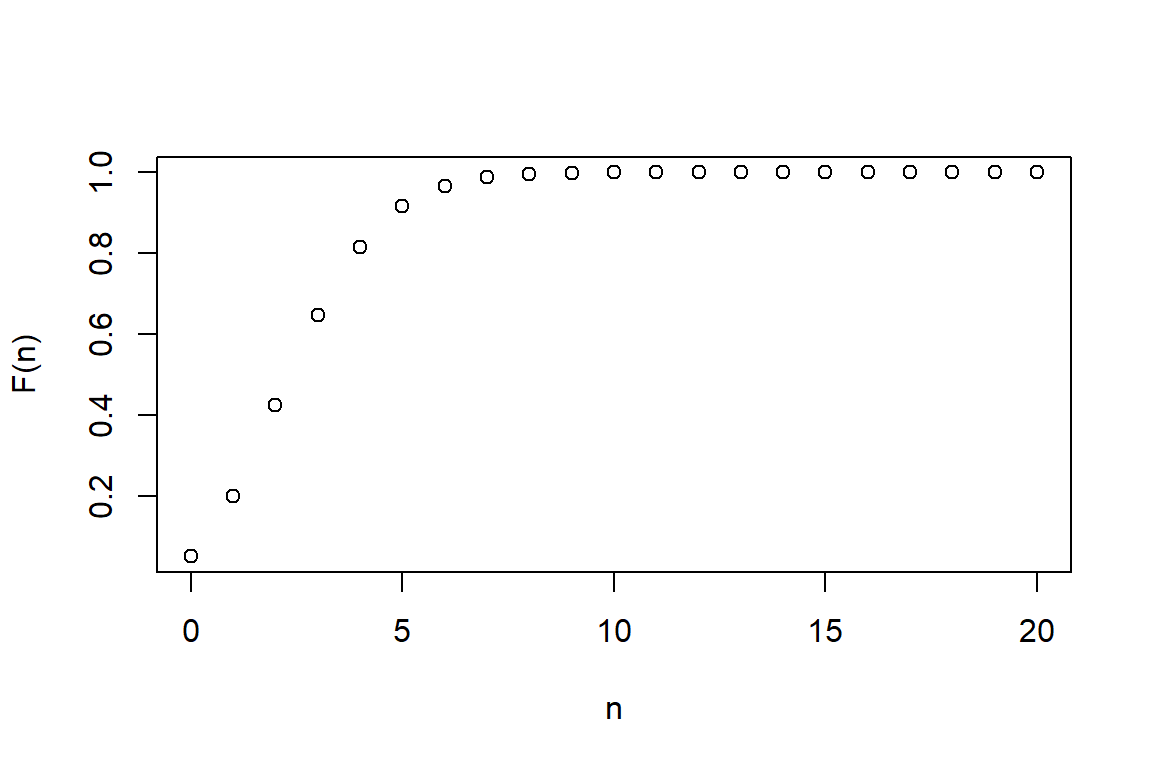
\includegraphics{R_for_Loss_Data_Analytics_files/figure-latex/unnamed-chunk-4-1} \end{center}

A few quick notes on these commands:

\begin{itemize}
\item
  The \texttt{par(mfrow)} function is handy for creating a simple
  multi-paneled plot. \texttt{mfrow} is a vector of length 2, where the
  first argument specifies the number of rows and the second the number
  of columns of plots.
\item
  The \texttt{hist()} computes a histogram of the given data values. You
  put the name of your dataset in between the parentheses of this
  function.
\end{itemize}

\subsection{Rating Variables}\label{rating-variables}

Earlier we considered a sample of 1,110 observations which may seem like
a lot. However, as we will seen in our forthcoming applications, because
of the preponderance of zeros and the skewed nature of claims, actuaries
typically yearn for more data. One common approach that we adopt here is
to examine outcomes from multiple years, thus increasing the sample
size.

\subsubsection{Average Claims Over Time}\label{average-claims-over-time}

Table 1.4 shows that the average claim varies over time.

Table 1.4

\begin{Shaded}
\begin{Highlighting}[]
\KeywordTok{library}\NormalTok{(doBy)}
\NormalTok{t_1a <-}\StringTok{ }\KeywordTok{summaryBy}\NormalTok{(Freq }\OperatorTok{~}\StringTok{ }\NormalTok{Year, }\DataTypeTok{data =}\NormalTok{ in_sample,   }
                 \DataTypeTok{FUN =} \ControlFlowTok{function}\NormalTok{ (x) \{ }\KeywordTok{c}\NormalTok{(}\DataTypeTok{m =} \KeywordTok{mean}\NormalTok{(x), }\DataTypeTok{num =} \KeywordTok{length}\NormalTok{(x)) \} )}
\NormalTok{t_1b <-}\StringTok{ }\KeywordTok{summaryBy}\NormalTok{(yAvg }\OperatorTok{~}\StringTok{ }\NormalTok{Year, }\DataTypeTok{data =}\NormalTok{ in_sample,   }
                 \DataTypeTok{FUN =} \ControlFlowTok{function}\NormalTok{ (x) \{ }\KeywordTok{c}\NormalTok{(}\DataTypeTok{m =} \KeywordTok{mean}\NormalTok{(x), }\DataTypeTok{num =} \KeywordTok{length}\NormalTok{(x)) \} )}
\NormalTok{t_1c <-}\StringTok{ }\KeywordTok{summaryBy}\NormalTok{(BCcov }\OperatorTok{~}\StringTok{ }\NormalTok{Year, }\DataTypeTok{data =}\NormalTok{ in_sample,   }
                 \DataTypeTok{FUN =} \ControlFlowTok{function}\NormalTok{ (x) \{ }\KeywordTok{c}\NormalTok{(}\DataTypeTok{m =} \KeywordTok{mean}\NormalTok{(x), }\DataTypeTok{num =} \KeywordTok{length}\NormalTok{(x)) \} )}
\NormalTok{table1_in <-}\StringTok{ }\KeywordTok{cbind}\NormalTok{(t_1a[}\DecValTok{1}\NormalTok{], t_1a[}\DecValTok{2}\NormalTok{], t_1b[}\DecValTok{2}\NormalTok{], t_1c[}\DecValTok{2}\NormalTok{], t_1a[}\DecValTok{3}\NormalTok{])}
\KeywordTok{names}\NormalTok{(table1_in) <-}\StringTok{ }\KeywordTok{c}\NormalTok{(}\StringTok{"Year"}\NormalTok{, }\StringTok{"Average Freq"}\NormalTok{, }\StringTok{"Average Sev"}\NormalTok{, }\StringTok{"Average Coverage"}\NormalTok{, }
                      \StringTok{"No. of Policyholders"}\NormalTok{)}
\KeywordTok{pander}\NormalTok{(table1_in)}
\end{Highlighting}
\end{Shaded}

\begin{longtable}[]{@{}ccccc@{}}
\toprule
\begin{minipage}[b]{0.08\columnwidth}\centering\strut
Year\strut
\end{minipage} & \begin{minipage}[b]{0.17\columnwidth}\centering\strut
Average Freq\strut
\end{minipage} & \begin{minipage}[b]{0.16\columnwidth}\centering\strut
Average Sev\strut
\end{minipage} & \begin{minipage}[b]{0.21\columnwidth}\centering\strut
Average Coverage\strut
\end{minipage} & \begin{minipage}[b]{0.25\columnwidth}\centering\strut
No. of Policyholders\strut
\end{minipage}\tabularnewline
\midrule
\endhead
\begin{minipage}[t]{0.08\columnwidth}\centering\strut
2006\strut
\end{minipage} & \begin{minipage}[t]{0.17\columnwidth}\centering\strut
0.9515\strut
\end{minipage} & \begin{minipage}[t]{0.16\columnwidth}\centering\strut
9695\strut
\end{minipage} & \begin{minipage}[t]{0.21\columnwidth}\centering\strut
32498186\strut
\end{minipage} & \begin{minipage}[t]{0.25\columnwidth}\centering\strut
1154\strut
\end{minipage}\tabularnewline
\begin{minipage}[t]{0.08\columnwidth}\centering\strut
2007\strut
\end{minipage} & \begin{minipage}[t]{0.17\columnwidth}\centering\strut
1.167\strut
\end{minipage} & \begin{minipage}[t]{0.16\columnwidth}\centering\strut
6544\strut
\end{minipage} & \begin{minipage}[t]{0.21\columnwidth}\centering\strut
35275949\strut
\end{minipage} & \begin{minipage}[t]{0.25\columnwidth}\centering\strut
1138\strut
\end{minipage}\tabularnewline
\begin{minipage}[t]{0.08\columnwidth}\centering\strut
2008\strut
\end{minipage} & \begin{minipage}[t]{0.17\columnwidth}\centering\strut
0.9742\strut
\end{minipage} & \begin{minipage}[t]{0.16\columnwidth}\centering\strut
5311\strut
\end{minipage} & \begin{minipage}[t]{0.21\columnwidth}\centering\strut
37267485\strut
\end{minipage} & \begin{minipage}[t]{0.25\columnwidth}\centering\strut
1125\strut
\end{minipage}\tabularnewline
\begin{minipage}[t]{0.08\columnwidth}\centering\strut
2009\strut
\end{minipage} & \begin{minipage}[t]{0.17\columnwidth}\centering\strut
1.219\strut
\end{minipage} & \begin{minipage}[t]{0.16\columnwidth}\centering\strut
4572\strut
\end{minipage} & \begin{minipage}[t]{0.21\columnwidth}\centering\strut
40355382\strut
\end{minipage} & \begin{minipage}[t]{0.25\columnwidth}\centering\strut
1112\strut
\end{minipage}\tabularnewline
\begin{minipage}[t]{0.08\columnwidth}\centering\strut
2010\strut
\end{minipage} & \begin{minipage}[t]{0.17\columnwidth}\centering\strut
1.241\strut
\end{minipage} & \begin{minipage}[t]{0.16\columnwidth}\centering\strut
20452\strut
\end{minipage} & \begin{minipage}[t]{0.21\columnwidth}\centering\strut
41242070\strut
\end{minipage} & \begin{minipage}[t]{0.25\columnwidth}\centering\strut
1110\strut
\end{minipage}\tabularnewline
\bottomrule
\end{longtable}

A few quick notes on these commands:

\begin{itemize}
\item
  The \texttt{summaryBy()} function provides summary statistics of a
  variable across different groups. You need to install the
  \texttt{doBy} package to use the command.
\item
  The \texttt{cbind()} combines vector, matrix or data frame arguments
  by columns. The row number of the two datasets must be equal.
\item
  The \texttt{c()} function combines its arguments to form a vector.
\end{itemize}

\subsubsection{Frequency and Claims Statistics of Full
Data}\label{frequency-and-claims-statistics-of-full-data}

For a different look at this five-year sample, Table 1.5 summarizes the
distribution of our two outcomes, frequency and claims amount. In each
case, the average exceeds the median, suggesting that the distributions
are right-skewed.

Table 1.5

\begin{Shaded}
\begin{Highlighting}[]
\NormalTok{BCcov.div1000 <-}\StringTok{ }\NormalTok{(in_sample}\OperatorTok{$}\NormalTok{BCcov) }\OperatorTok{/}\StringTok{ }\DecValTok{1000}

\NormalTok{t_}\DecValTok{1}\NormalTok{ <-}\StringTok{ }\KeywordTok{summaryBy}\NormalTok{(Freq }\OperatorTok{~}\StringTok{ }\DecValTok{1}\NormalTok{, }\DataTypeTok{data =}\NormalTok{ in_sample,}
          \DataTypeTok{FUN =} \ControlFlowTok{function}\NormalTok{ (x) \{ }\KeywordTok{c}\NormalTok{(}\DataTypeTok{ma =} \KeywordTok{min}\NormalTok{(x), }\DataTypeTok{m1 =} \KeywordTok{median}\NormalTok{(x), }\DataTypeTok{m =} \KeywordTok{mean}\NormalTok{(x), }\DataTypeTok{mb =} \KeywordTok{max}\NormalTok{(x)) \} )}
\KeywordTok{names}\NormalTok{(t_}\DecValTok{1}\NormalTok{) <-}\StringTok{ }\KeywordTok{c}\NormalTok{(}\StringTok{"Minimum"}\NormalTok{, }\StringTok{"Median"}\NormalTok{, }\StringTok{"Average"}\NormalTok{, }\StringTok{"Maximum"}\NormalTok{)}
\NormalTok{t_}\DecValTok{2}\NormalTok{ <-}\StringTok{ }\KeywordTok{summaryBy}\NormalTok{(yAvg }\OperatorTok{~}\StringTok{ }\DecValTok{1}\NormalTok{, }\DataTypeTok{data =}\NormalTok{ in_sample, }
          \DataTypeTok{FUN =} \ControlFlowTok{function}\NormalTok{ (x) \{ }\KeywordTok{c}\NormalTok{(}\DataTypeTok{ma =} \KeywordTok{min}\NormalTok{(x), }\DataTypeTok{m1 =} \KeywordTok{median}\NormalTok{(x), }\DataTypeTok{m =} \KeywordTok{mean}\NormalTok{(x), }\DataTypeTok{mb =} \KeywordTok{max}\NormalTok{(x)) \} )}
\KeywordTok{names}\NormalTok{(t_}\DecValTok{2}\NormalTok{) <-}\StringTok{ }\KeywordTok{c}\NormalTok{(}\StringTok{"Minimum"}\NormalTok{, }\StringTok{"Median"}\NormalTok{, }\StringTok{"Average"}\NormalTok{, }\StringTok{"Maximum"}\NormalTok{)}
\NormalTok{t_}\DecValTok{3}\NormalTok{ <-}\StringTok{ }\KeywordTok{summaryBy}\NormalTok{(Deduct }\OperatorTok{~}\StringTok{ }\DecValTok{1}\NormalTok{, }\DataTypeTok{data =}\NormalTok{ in_sample, }
          \DataTypeTok{FUN =} \ControlFlowTok{function}\NormalTok{ (x) \{ }\KeywordTok{c}\NormalTok{(}\DataTypeTok{ma =} \KeywordTok{min}\NormalTok{(x), }\DataTypeTok{m1 =} \KeywordTok{median}\NormalTok{(x), }\DataTypeTok{m =} \KeywordTok{mean}\NormalTok{(x), }\DataTypeTok{mb =} \KeywordTok{max}\NormalTok{(x)) \} )}
\KeywordTok{names}\NormalTok{(t_}\DecValTok{3}\NormalTok{) <-}\StringTok{ }\KeywordTok{c}\NormalTok{(}\StringTok{"Minimum"}\NormalTok{, }\StringTok{"Median"}\NormalTok{, }\StringTok{"Average"}\NormalTok{, }\StringTok{"Maximum"}\NormalTok{)}
\NormalTok{t_}\DecValTok{4}\NormalTok{ <-}\StringTok{ }\KeywordTok{summaryBy}\NormalTok{(BCcov.div1000 }\OperatorTok{~}\StringTok{ }\DecValTok{1}\NormalTok{, }\DataTypeTok{data =}\NormalTok{ in_sample, }
          \DataTypeTok{FUN =} \ControlFlowTok{function}\NormalTok{ (x) \{ }\KeywordTok{c}\NormalTok{(}\DataTypeTok{ma =} \KeywordTok{min}\NormalTok{(x), }\DataTypeTok{m1 =} \KeywordTok{median}\NormalTok{(x), }\DataTypeTok{m =} \KeywordTok{mean}\NormalTok{(x), }\DataTypeTok{mb =} \KeywordTok{max}\NormalTok{(x)) \} )}
\KeywordTok{names}\NormalTok{(t_}\DecValTok{4}\NormalTok{) <-}\StringTok{ }\KeywordTok{c}\NormalTok{(}\StringTok{"Minimum"}\NormalTok{, }\StringTok{"Median"}\NormalTok{,}\StringTok{"Average"}\NormalTok{, }\StringTok{"Maximum"}\NormalTok{)}
\NormalTok{table_}\DecValTok{2}\NormalTok{ <-}\StringTok{ }\KeywordTok{rbind}\NormalTok{(t_}\DecValTok{1}\NormalTok{, t_}\DecValTok{2}\NormalTok{, t_}\DecValTok{3}\NormalTok{, t_}\DecValTok{4}\NormalTok{)}
\NormalTok{table_2a <-}\StringTok{ }\KeywordTok{round}\NormalTok{(table_}\DecValTok{2}\NormalTok{, }\DecValTok{3}\NormalTok{)}
\NormalTok{row_label <-}\StringTok{ }\KeywordTok{rbind}\NormalTok{(}\StringTok{"Claim Frequency"}\NormalTok{, }\StringTok{"Claim Severity"}\NormalTok{, }\StringTok{"Deductible"}\NormalTok{, }\StringTok{"Coverage (000's)"}\NormalTok{)}
\NormalTok{table_2aa <-}\StringTok{ }\KeywordTok{cbind}\NormalTok{(row_label, }\KeywordTok{as.matrix}\NormalTok{(table_2a))}
\KeywordTok{pander}\NormalTok{(table_2aa)}
\end{Highlighting}
\end{Shaded}

\begin{longtable}[]{@{}ccccc@{}}
\toprule
\begin{minipage}[b]{0.23\columnwidth}\centering\strut
~\strut
\end{minipage} & \begin{minipage}[b]{0.12\columnwidth}\centering\strut
Minimum\strut
\end{minipage} & \begin{minipage}[b]{0.14\columnwidth}\centering\strut
Median\strut
\end{minipage} & \begin{minipage}[b]{0.14\columnwidth}\centering\strut
Average\strut
\end{minipage} & \begin{minipage}[b]{0.16\columnwidth}\centering\strut
Maximum\strut
\end{minipage}\tabularnewline
\midrule
\endhead
\begin{minipage}[t]{0.23\columnwidth}\centering\strut
Claim Frequency\strut
\end{minipage} & \begin{minipage}[t]{0.12\columnwidth}\centering\strut
0\strut
\end{minipage} & \begin{minipage}[t]{0.14\columnwidth}\centering\strut
0\strut
\end{minipage} & \begin{minipage}[t]{0.14\columnwidth}\centering\strut
1.109\strut
\end{minipage} & \begin{minipage}[t]{0.16\columnwidth}\centering\strut
263\strut
\end{minipage}\tabularnewline
\begin{minipage}[t]{0.23\columnwidth}\centering\strut
Claim Severity\strut
\end{minipage} & \begin{minipage}[t]{0.12\columnwidth}\centering\strut
0\strut
\end{minipage} & \begin{minipage}[t]{0.14\columnwidth}\centering\strut
0\strut
\end{minipage} & \begin{minipage}[t]{0.14\columnwidth}\centering\strut
9291.565\strut
\end{minipage} & \begin{minipage}[t]{0.16\columnwidth}\centering\strut
12922217.84\strut
\end{minipage}\tabularnewline
\begin{minipage}[t]{0.23\columnwidth}\centering\strut
Deductible\strut
\end{minipage} & \begin{minipage}[t]{0.12\columnwidth}\centering\strut
500\strut
\end{minipage} & \begin{minipage}[t]{0.14\columnwidth}\centering\strut
1000\strut
\end{minipage} & \begin{minipage}[t]{0.14\columnwidth}\centering\strut
3364.87\strut
\end{minipage} & \begin{minipage}[t]{0.16\columnwidth}\centering\strut
1e+05\strut
\end{minipage}\tabularnewline
\begin{minipage}[t]{0.23\columnwidth}\centering\strut
Coverage (000's)\strut
\end{minipage} & \begin{minipage}[t]{0.12\columnwidth}\centering\strut
8.937\strut
\end{minipage} & \begin{minipage}[t]{0.14\columnwidth}\centering\strut
11353.566\strut
\end{minipage} & \begin{minipage}[t]{0.14\columnwidth}\centering\strut
37280.855\strut
\end{minipage} & \begin{minipage}[t]{0.16\columnwidth}\centering\strut
2444796.98\strut
\end{minipage}\tabularnewline
\bottomrule
\end{longtable}

A few quick notes on these commands:

\begin{itemize}
\item
  The \texttt{rbind()} combines vector, matrix or data frame arguments
  by rows. The column of the two datasets must be same.
\item
  The \texttt{round()} function rounds the values in its first argument
  to the specified number of decimal places (default 0).
\end{itemize}

\subsubsection{Rating Variable
Description}\label{rating-variable-description}

Table 1.6 describes the rating variables considered in this chapter. To
handle the skewness, we henceforth focus on logarithmic transformations
of coverage and deductibles. See table 1.6 below for variables and
variable descriptions.

Table 1.6

\begin{Shaded}
\begin{Highlighting}[]
\NormalTok{des <-}\StringTok{ }\KeywordTok{read.table}\NormalTok{(}\DataTypeTok{header =} \OtherTok{TRUE}\NormalTok{, }\DataTypeTok{text =} \StringTok{'}
\StringTok{ Variable Description}
\StringTok{  "BCcov"  "Total building and content coverage in dollars"}
\StringTok{  "Deduct"  "Deductible in dollars"}
\StringTok{"Entity Type"   "Categorical variable that is one of six types: }
\StringTok{(Village, City, County, Misc, School, or Town)"}
\StringTok{"alarm_credit"  "Categorical variable that is one of four types: }
\StringTok{(0%, 5%, 10%, or 15%), for automatic smoke alarms in main rooms"}
\StringTok{"NoClaimCredit" "Binary variable to indicate no claims in the past two years"}
\StringTok{"Fire5" "Binary variable to indicate the fire class is below 5. }
\StringTok{(The range of fire class is 0~10)" '}\NormalTok{)}
\end{Highlighting}
\end{Shaded}

\begin{Shaded}
\begin{Highlighting}[]
\KeywordTok{pander}\NormalTok{(des)}
\end{Highlighting}
\end{Shaded}

\begin{longtable}[]{@{}cc@{}}
\toprule
\begin{minipage}[b]{0.21\columnwidth}\centering\strut
Variable\strut
\end{minipage} & \begin{minipage}[b]{0.42\columnwidth}\centering\strut
Description\strut
\end{minipage}\tabularnewline
\midrule
\endhead
\begin{minipage}[t]{0.21\columnwidth}\centering\strut
BCcov\strut
\end{minipage} & \begin{minipage}[t]{0.42\columnwidth}\centering\strut
Total building and content coverage in dollars\strut
\end{minipage}\tabularnewline
\begin{minipage}[t]{0.21\columnwidth}\centering\strut
Deduct\strut
\end{minipage} & \begin{minipage}[t]{0.42\columnwidth}\centering\strut
Deductible in dollars\strut
\end{minipage}\tabularnewline
\begin{minipage}[t]{0.21\columnwidth}\centering\strut
Entity Type\strut
\end{minipage} & \begin{minipage}[t]{0.42\columnwidth}\centering\strut
Categorical variable that is one of six types: (Village, City, County,
Misc, School, or Town)\strut
\end{minipage}\tabularnewline
\begin{minipage}[t]{0.21\columnwidth}\centering\strut
alarm\_credit\strut
\end{minipage} & \begin{minipage}[t]{0.42\columnwidth}\centering\strut
Categorical variable that is one of four types: (0\%, 5\%, 10\%, or
15\%), for automatic smoke alarms in main rooms\strut
\end{minipage}\tabularnewline
\begin{minipage}[t]{0.21\columnwidth}\centering\strut
NoClaimCredit\strut
\end{minipage} & \begin{minipage}[t]{0.42\columnwidth}\centering\strut
Binary variable to indicate no claims in the past two years\strut
\end{minipage}\tabularnewline
\begin{minipage}[t]{0.21\columnwidth}\centering\strut
Fire5\strut
\end{minipage} & \begin{minipage}[t]{0.42\columnwidth}\centering\strut
Binary variable to indicate the fire class is below 5. (The range of
fire class is 0\textasciitilde{}10)\strut
\end{minipage}\tabularnewline
\bottomrule
\end{longtable}

\subsubsection{Frequency and Claims by Rating
Variables}\label{frequency-and-claims-by-rating-variables}

To get a sense of the relationship between the non-continuous rating
variables and claims, Table 1.7 relates the claims outcomes to these
categorical variables. Table 1.7 shows claims summary by Entity Type,
Fire Class, and No Claim Credit.

Table 1.7

\begin{Shaded}
\begin{Highlighting}[]
\CommentTok{# Table 1.7}
\NormalTok{by_var_summ <-}\StringTok{ }\ControlFlowTok{function}\NormalTok{ (datasub) \{}
\NormalTok{  temp_a <-}\StringTok{ }\KeywordTok{summaryBy}\NormalTok{(Freq }\OperatorTok{~}\StringTok{ }\DecValTok{1}\NormalTok{ , }\DataTypeTok{data =}\NormalTok{ datasub,   }
                      \DataTypeTok{FUN =} \ControlFlowTok{function}\NormalTok{ (x) \{ }\KeywordTok{c}\NormalTok{(}\DataTypeTok{m =} \KeywordTok{mean}\NormalTok{(x), }\DataTypeTok{num =} \KeywordTok{length}\NormalTok{(x)) \} )}
\NormalTok{  datasub_}\DecValTok{1}\NormalTok{ <-}\StringTok{ }\KeywordTok{subset}\NormalTok{(datasub, yAvg }\OperatorTok{>}\StringTok{ }\DecValTok{0}\NormalTok{)}
\NormalTok{  temp_b <-}\StringTok{ }\KeywordTok{summaryBy}\NormalTok{(yAvg }\OperatorTok{~}\StringTok{ }\DecValTok{1}\NormalTok{, }\DataTypeTok{data =}\NormalTok{ datasub_}\DecValTok{1}\NormalTok{,}
                      \DataTypeTok{FUN =} \ControlFlowTok{function}\NormalTok{ (x) \{ }\KeywordTok{c}\NormalTok{(}\DataTypeTok{m =} \KeywordTok{mean}\NormalTok{(x)) \} )}
\NormalTok{  temp_c <-}\StringTok{ }\KeywordTok{merge}\NormalTok{(temp_a, temp_b, }\DataTypeTok{all.x =}\NormalTok{ T)[}\KeywordTok{c}\NormalTok{(}\DecValTok{2}\NormalTok{, }\DecValTok{1}\NormalTok{, }\DecValTok{3}\NormalTok{)]}
\NormalTok{  temp_c1 <-}\StringTok{ }\KeywordTok{as.matrix}\NormalTok{(temp_c)}
  \KeywordTok{return}\NormalTok{(temp_c1)}
\NormalTok{\}}

\NormalTok{datasub <-}\StringTok{ }\KeywordTok{subset}\NormalTok{(in_sample, TypeVillage }\OperatorTok{==}\StringTok{ }\DecValTok{1}\NormalTok{);   }
\NormalTok{t_}\DecValTok{1}\NormalTok{ <-}\StringTok{ }\KeywordTok{by_var_summ}\NormalTok{(datasub)}
\NormalTok{datasub <-}\StringTok{ }\KeywordTok{subset}\NormalTok{(in_sample, TypeCity }\OperatorTok{==}\StringTok{ }\DecValTok{1}\NormalTok{);      }
\NormalTok{t_}\DecValTok{2}\NormalTok{ <-}\StringTok{ }\KeywordTok{by_var_summ}\NormalTok{(datasub)}
\NormalTok{datasub <-}\StringTok{ }\KeywordTok{subset}\NormalTok{(in_sample, TypeCounty }\OperatorTok{==}\StringTok{ }\DecValTok{1}\NormalTok{);   }
\NormalTok{t_}\DecValTok{3}\NormalTok{ <-}\StringTok{ }\KeywordTok{by_var_summ}\NormalTok{(datasub)}
\NormalTok{datasub <-}\StringTok{ }\KeywordTok{subset}\NormalTok{(in_sample, TypeMisc }\OperatorTok{==}\StringTok{ }\DecValTok{1}\NormalTok{);      }
\NormalTok{t_}\DecValTok{4}\NormalTok{ <-}\StringTok{ }\KeywordTok{by_var_summ}\NormalTok{(datasub)}
\NormalTok{datasub <-}\StringTok{ }\KeywordTok{subset}\NormalTok{(in_sample, TypeSchool }\OperatorTok{==}\StringTok{ }\DecValTok{1}\NormalTok{);    }
\NormalTok{t_}\DecValTok{5}\NormalTok{ <-}\StringTok{ }\KeywordTok{by_var_summ}\NormalTok{(datasub)}
\NormalTok{datasub <-}\StringTok{ }\KeywordTok{subset}\NormalTok{(in_sample, TypeTown }\OperatorTok{==}\StringTok{ }\DecValTok{1}\NormalTok{);      }
\NormalTok{t_}\DecValTok{6}\NormalTok{ <-}\StringTok{ }\KeywordTok{by_var_summ}\NormalTok{(datasub)}
\NormalTok{datasub <-}\StringTok{ }\KeywordTok{subset}\NormalTok{(in_sample, Fire5 }\OperatorTok{==}\StringTok{ }\DecValTok{0}\NormalTok{);                      }
\NormalTok{t_}\DecValTok{7}\NormalTok{ <-}\StringTok{ }\KeywordTok{by_var_summ}\NormalTok{(datasub)}
\NormalTok{datasub <-}\StringTok{ }\KeywordTok{subset}\NormalTok{(in_sample, Fire5 }\OperatorTok{==}\StringTok{ }\DecValTok{1}\NormalTok{);                      }
\NormalTok{t_}\DecValTok{8}\NormalTok{ <-}\StringTok{ }\KeywordTok{by_var_summ}\NormalTok{(datasub)}
\NormalTok{datasub <-}\StringTok{ }\KeywordTok{subset}\NormalTok{(in_sample, in_sample}\OperatorTok{$}\NormalTok{NoClaimCredit }\OperatorTok{==}\StringTok{ }\DecValTok{0}\NormalTok{);}
\NormalTok{t_}\DecValTok{9}\NormalTok{ <-}\StringTok{ }\KeywordTok{by_var_summ}\NormalTok{(datasub)}
\NormalTok{datasub <-}\StringTok{ }\KeywordTok{subset}\NormalTok{(in_sample, in_sample}\OperatorTok{$}\NormalTok{NoClaimCredit }\OperatorTok{==}\StringTok{ }\DecValTok{1}\NormalTok{);}
\NormalTok{t_}\DecValTok{10}\NormalTok{ <-}\StringTok{ }\KeywordTok{by_var_summ}\NormalTok{(datasub)}
\NormalTok{t_}\DecValTok{11}\NormalTok{ <-}\StringTok{ }\KeywordTok{by_var_summ}\NormalTok{(in_sample)}

\NormalTok{table_a <-}\StringTok{ }\KeywordTok{rbind}\NormalTok{(t_}\DecValTok{1}\NormalTok{, t_}\DecValTok{2}\NormalTok{, t_}\DecValTok{3}\NormalTok{, t_}\DecValTok{4}\NormalTok{, t_}\DecValTok{5}\NormalTok{, t_}\DecValTok{6}\NormalTok{, t_}\DecValTok{7}\NormalTok{, t_}\DecValTok{8}\NormalTok{, t_}\DecValTok{9}\NormalTok{, t_}\DecValTok{10}\NormalTok{, t_}\DecValTok{11}\NormalTok{)}
\NormalTok{table_aa <-}\StringTok{ }\KeywordTok{round}\NormalTok{(table_a, }\DecValTok{3}\NormalTok{)}
\NormalTok{row_label <-}\StringTok{ }\KeywordTok{rbind}\NormalTok{(}\StringTok{"Village"}\NormalTok{, }\StringTok{"City"}\NormalTok{, }\StringTok{"County"}\NormalTok{, }\StringTok{"Misc"}\NormalTok{, }\StringTok{"School"}\NormalTok{,}
                  \StringTok{"Town"}\NormalTok{, }\StringTok{"Fire5--No"}\NormalTok{, }\StringTok{"Fire5--Yes"}\NormalTok{, }\StringTok{"NoClaimCredit--No"}\NormalTok{, }
                  \StringTok{"NoClaimCredit--Yes"}\NormalTok{, }\StringTok{"Total"}\NormalTok{)}
\NormalTok{table_}\DecValTok{4}\NormalTok{ <-}\StringTok{ }\KeywordTok{cbind}\NormalTok{(row_label, }\KeywordTok{as.matrix}\NormalTok{(table_aa))}
\end{Highlighting}
\end{Shaded}

\begin{Shaded}
\begin{Highlighting}[]
\KeywordTok{pander}\NormalTok{(table_}\DecValTok{4}\NormalTok{)}
\end{Highlighting}
\end{Shaded}

\begin{longtable}[]{@{}cccc@{}}
\toprule
\begin{minipage}[b]{0.26\columnwidth}\centering\strut
~\strut
\end{minipage} & \begin{minipage}[b]{0.14\columnwidth}\centering\strut
Freq.num\strut
\end{minipage} & \begin{minipage}[b]{0.11\columnwidth}\centering\strut
Freq.m\strut
\end{minipage} & \begin{minipage}[b]{0.14\columnwidth}\centering\strut
yAvg.m\strut
\end{minipage}\tabularnewline
\midrule
\endhead
\begin{minipage}[t]{0.26\columnwidth}\centering\strut
Village\strut
\end{minipage} & \begin{minipage}[t]{0.14\columnwidth}\centering\strut
1341\strut
\end{minipage} & \begin{minipage}[t]{0.11\columnwidth}\centering\strut
0.452\strut
\end{minipage} & \begin{minipage}[t]{0.14\columnwidth}\centering\strut
10645.206\strut
\end{minipage}\tabularnewline
\begin{minipage}[t]{0.26\columnwidth}\centering\strut
City\strut
\end{minipage} & \begin{minipage}[t]{0.14\columnwidth}\centering\strut
793\strut
\end{minipage} & \begin{minipage}[t]{0.11\columnwidth}\centering\strut
1.941\strut
\end{minipage} & \begin{minipage}[t]{0.14\columnwidth}\centering\strut
16924.035\strut
\end{minipage}\tabularnewline
\begin{minipage}[t]{0.26\columnwidth}\centering\strut
County\strut
\end{minipage} & \begin{minipage}[t]{0.14\columnwidth}\centering\strut
328\strut
\end{minipage} & \begin{minipage}[t]{0.11\columnwidth}\centering\strut
4.899\strut
\end{minipage} & \begin{minipage}[t]{0.14\columnwidth}\centering\strut
15453.206\strut
\end{minipage}\tabularnewline
\begin{minipage}[t]{0.26\columnwidth}\centering\strut
Misc\strut
\end{minipage} & \begin{minipage}[t]{0.14\columnwidth}\centering\strut
609\strut
\end{minipage} & \begin{minipage}[t]{0.11\columnwidth}\centering\strut
0.186\strut
\end{minipage} & \begin{minipage}[t]{0.14\columnwidth}\centering\strut
43036.076\strut
\end{minipage}\tabularnewline
\begin{minipage}[t]{0.26\columnwidth}\centering\strut
School\strut
\end{minipage} & \begin{minipage}[t]{0.14\columnwidth}\centering\strut
1597\strut
\end{minipage} & \begin{minipage}[t]{0.11\columnwidth}\centering\strut
1.434\strut
\end{minipage} & \begin{minipage}[t]{0.14\columnwidth}\centering\strut
64346.394\strut
\end{minipage}\tabularnewline
\begin{minipage}[t]{0.26\columnwidth}\centering\strut
Town\strut
\end{minipage} & \begin{minipage}[t]{0.14\columnwidth}\centering\strut
971\strut
\end{minipage} & \begin{minipage}[t]{0.11\columnwidth}\centering\strut
0.103\strut
\end{minipage} & \begin{minipage}[t]{0.14\columnwidth}\centering\strut
19831.048\strut
\end{minipage}\tabularnewline
\begin{minipage}[t]{0.26\columnwidth}\centering\strut
Fire5--No\strut
\end{minipage} & \begin{minipage}[t]{0.14\columnwidth}\centering\strut
2508\strut
\end{minipage} & \begin{minipage}[t]{0.11\columnwidth}\centering\strut
0.502\strut
\end{minipage} & \begin{minipage}[t]{0.14\columnwidth}\centering\strut
13935.421\strut
\end{minipage}\tabularnewline
\begin{minipage}[t]{0.26\columnwidth}\centering\strut
Fire5--Yes\strut
\end{minipage} & \begin{minipage}[t]{0.14\columnwidth}\centering\strut
3131\strut
\end{minipage} & \begin{minipage}[t]{0.11\columnwidth}\centering\strut
1.596\strut
\end{minipage} & \begin{minipage}[t]{0.14\columnwidth}\centering\strut
41421.263\strut
\end{minipage}\tabularnewline
\begin{minipage}[t]{0.26\columnwidth}\centering\strut
NoClaimCredit--No\strut
\end{minipage} & \begin{minipage}[t]{0.14\columnwidth}\centering\strut
3786\strut
\end{minipage} & \begin{minipage}[t]{0.11\columnwidth}\centering\strut
1.501\strut
\end{minipage} & \begin{minipage}[t]{0.14\columnwidth}\centering\strut
31365.085\strut
\end{minipage}\tabularnewline
\begin{minipage}[t]{0.26\columnwidth}\centering\strut
NoClaimCredit--Yes\strut
\end{minipage} & \begin{minipage}[t]{0.14\columnwidth}\centering\strut
1853\strut
\end{minipage} & \begin{minipage}[t]{0.11\columnwidth}\centering\strut
0.31\strut
\end{minipage} & \begin{minipage}[t]{0.14\columnwidth}\centering\strut
30498.714\strut
\end{minipage}\tabularnewline
\begin{minipage}[t]{0.26\columnwidth}\centering\strut
Total\strut
\end{minipage} & \begin{minipage}[t]{0.14\columnwidth}\centering\strut
5639\strut
\end{minipage} & \begin{minipage}[t]{0.11\columnwidth}\centering\strut
1.109\strut
\end{minipage} & \begin{minipage}[t]{0.14\columnwidth}\centering\strut
31206.155\strut
\end{minipage}\tabularnewline
\bottomrule
\end{longtable}

Table 1.8 shows claims summary by Entity Type and Alarm Credit

Table 1.8

\begin{Shaded}
\begin{Highlighting}[]
\NormalTok{by_var_summ <-}\StringTok{ }\ControlFlowTok{function}\NormalTok{(datasub) \{}
\NormalTok{  temp_a <-}\StringTok{ }\KeywordTok{summaryBy}\NormalTok{(Freq }\OperatorTok{~}\StringTok{ }\NormalTok{AC00 , }\DataTypeTok{data =}\NormalTok{ datasub,   }
                     \DataTypeTok{FUN =} \ControlFlowTok{function}\NormalTok{(x) \{ }\KeywordTok{c}\NormalTok{(}\DataTypeTok{m =} \KeywordTok{mean}\NormalTok{(x), }\DataTypeTok{num =} \KeywordTok{length}\NormalTok{(x)) \} )}
\NormalTok{  datasub_}\DecValTok{1}\NormalTok{ <-}\StringTok{ }\KeywordTok{subset}\NormalTok{(datasub, yAvg }\OperatorTok{>}\StringTok{ }\DecValTok{0}\NormalTok{)}
  \ControlFlowTok{if}\NormalTok{ (}\KeywordTok{nrow}\NormalTok{(datasub_}\DecValTok{1}\NormalTok{) }\OperatorTok{==}\StringTok{ }\DecValTok{0}\NormalTok{) \{ n <-}\StringTok{ }\KeywordTok{nrow}\NormalTok{(datasub)}
    \KeywordTok{return}\NormalTok{(}\KeywordTok{c}\NormalTok{(}\DecValTok{0}\NormalTok{, }\DecValTok{0}\NormalTok{, n))}
\NormalTok{  \} }\ControlFlowTok{else} 
\NormalTok{  \{}
\NormalTok{    temp_b <-}\StringTok{ }\KeywordTok{summaryBy}\NormalTok{(yAvg }\OperatorTok{~}\StringTok{ }\NormalTok{AC00, }\DataTypeTok{data =}\NormalTok{ datasub_}\DecValTok{1}\NormalTok{,}
                       \DataTypeTok{FUN =} \ControlFlowTok{function}\NormalTok{(x) \{ }\KeywordTok{c}\NormalTok{(}\DataTypeTok{m =} \KeywordTok{mean}\NormalTok{(x)) \} )}
\NormalTok{    temp_c <-}\StringTok{ }\KeywordTok{merge}\NormalTok{(temp_a, temp_b, }\DataTypeTok{all.x =}\NormalTok{ T)[}\KeywordTok{c}\NormalTok{(}\DecValTok{2}\NormalTok{, }\DecValTok{4}\NormalTok{, }\DecValTok{3}\NormalTok{)]}
\NormalTok{    temp_c1 <-}\StringTok{ }\KeywordTok{as.matrix}\NormalTok{(temp_c)}
    \KeywordTok{return}\NormalTok{(temp_c1)}
\NormalTok{  \}}
\NormalTok{\}}
\NormalTok{alarm_c <-}\StringTok{ }\DecValTok{1} \OperatorTok{*}\StringTok{ }\NormalTok{(in_sample}\OperatorTok{$}\NormalTok{AC00 }\OperatorTok{==}\StringTok{ }\DecValTok{1}\NormalTok{) }\OperatorTok{+}\StringTok{ }\DecValTok{2} \OperatorTok{*}\StringTok{ }\NormalTok{(in_sample}\OperatorTok{$}\NormalTok{AC05 }\OperatorTok{==}\StringTok{ }\DecValTok{1}\NormalTok{) }\OperatorTok{+}\StringTok{ }
\StringTok{           }\DecValTok{3} \OperatorTok{*}\StringTok{ }\NormalTok{(in_sample}\OperatorTok{$}\NormalTok{AC10 }\OperatorTok{==}\StringTok{ }\DecValTok{1}\NormalTok{) }\OperatorTok{+}\StringTok{ }\DecValTok{4} \OperatorTok{*}\StringTok{ }\NormalTok{(in_sample}\OperatorTok{$}\NormalTok{AC15 }\OperatorTok{==}\StringTok{ }\DecValTok{1}\NormalTok{)}
\NormalTok{by_var_credit<-}\ControlFlowTok{function}\NormalTok{(ACnum)\{}
\NormalTok{datasub <-}\StringTok{  }\KeywordTok{subset}\NormalTok{(in_sample, TypeVillage }\OperatorTok{==}\StringTok{ }\DecValTok{1} \OperatorTok{&}\StringTok{ }\NormalTok{alarm_c }\OperatorTok{==}\StringTok{ }\NormalTok{ACnum); }
\NormalTok{t_}\DecValTok{1}\NormalTok{ <-}\StringTok{ }\KeywordTok{by_var_summ}\NormalTok{(datasub)}
\NormalTok{datasub <-}\StringTok{  }\KeywordTok{subset}\NormalTok{(in_sample, TypeCity }\OperatorTok{==}\StringTok{ }\DecValTok{1} \OperatorTok{&}\StringTok{ }\NormalTok{alarm_c }\OperatorTok{==}\StringTok{ }\NormalTok{ACnum);      }
\NormalTok{t_}\DecValTok{2}\NormalTok{ <-}\StringTok{ }\KeywordTok{by_var_summ}\NormalTok{(datasub)}
\NormalTok{datasub <-}\StringTok{  }\KeywordTok{subset}\NormalTok{(in_sample, TypeCounty }\OperatorTok{==}\StringTok{ }\DecValTok{1} \OperatorTok{&}\StringTok{ }\NormalTok{alarm_c }\OperatorTok{==}\StringTok{ }\NormalTok{ACnum);   }
\NormalTok{t_}\DecValTok{3}\NormalTok{ <-}\StringTok{ }\KeywordTok{by_var_summ}\NormalTok{(datasub)}
\NormalTok{datasub <-}\StringTok{  }\KeywordTok{subset}\NormalTok{(in_sample, TypeMisc }\OperatorTok{==}\StringTok{ }\DecValTok{1} \OperatorTok{&}\StringTok{ }\NormalTok{alarm_c }\OperatorTok{==}\StringTok{ }\NormalTok{ACnum);}
\NormalTok{t_}\DecValTok{4}\NormalTok{ <-}\StringTok{ }\KeywordTok{by_var_summ}\NormalTok{(datasub)}
\NormalTok{datasub <-}\StringTok{  }\KeywordTok{subset}\NormalTok{(in_sample, TypeSchool }\OperatorTok{==}\StringTok{ }\DecValTok{1} \OperatorTok{&}\StringTok{ }\NormalTok{alarm_c }\OperatorTok{==}\StringTok{ }\NormalTok{ACnum);    }
\NormalTok{t_}\DecValTok{5}\NormalTok{ <-}\StringTok{ }\KeywordTok{by_var_summ}\NormalTok{(datasub)}
\NormalTok{datasub <-}\StringTok{  }\KeywordTok{subset}\NormalTok{(in_sample, TypeTown }\OperatorTok{==}\StringTok{ }\DecValTok{1} \OperatorTok{&}\StringTok{ }\NormalTok{alarm_c }\OperatorTok{==}\NormalTok{ACnum);      }
\NormalTok{t_}\DecValTok{6}\NormalTok{ <-}\StringTok{ }\KeywordTok{by_var_summ}\NormalTok{(datasub)}
\NormalTok{datasub <-}\StringTok{  }\KeywordTok{subset}\NormalTok{(in_sample, alarm_c }\OperatorTok{==}\StringTok{ }\NormalTok{ACnum);  }
\NormalTok{t_}\DecValTok{7}\NormalTok{ <-}\StringTok{ }\KeywordTok{by_var_summ}\NormalTok{(datasub)}
\NormalTok{table_a <-}\StringTok{ }\KeywordTok{rbind}\NormalTok{(t_}\DecValTok{1}\NormalTok{, t_}\DecValTok{2}\NormalTok{, t_}\DecValTok{3}\NormalTok{, t_}\DecValTok{4}\NormalTok{, t_}\DecValTok{5}\NormalTok{, t_}\DecValTok{6}\NormalTok{, t_}\DecValTok{7}\NormalTok{)}
\NormalTok{table_aa <-}\StringTok{ }\KeywordTok{round}\NormalTok{(table_a, }\DecValTok{3}\NormalTok{)}
\NormalTok{row_label <-}\StringTok{ }\KeywordTok{rbind}\NormalTok{(}\StringTok{"Village"}\NormalTok{, }\StringTok{"City"}\NormalTok{, }\StringTok{"County"}\NormalTok{, }\StringTok{"Misc"}\NormalTok{, }\StringTok{"School"}\NormalTok{, }\StringTok{"Town"}\NormalTok{,}\StringTok{"Total"}\NormalTok{)}
\NormalTok{table_}\DecValTok{4}\NormalTok{ <-}\StringTok{ }\KeywordTok{cbind}\NormalTok{(row_label,}\KeywordTok{as.matrix}\NormalTok{(table_aa))}
\NormalTok{\}}
\NormalTok{table_4a <-}\StringTok{ }\KeywordTok{by_var_credit}\NormalTok{(}\DecValTok{1}\NormalTok{)  }\CommentTok{# claims summary by entity type and alarm credit == 00}
\NormalTok{table_4b <-}\StringTok{ }\KeywordTok{by_var_credit}\NormalTok{(}\DecValTok{2}\NormalTok{)  }\CommentTok{# claims summary by entity type and alarm credit == 05 }
\NormalTok{table_4c <-}\StringTok{ }\KeywordTok{by_var_credit}\NormalTok{(}\DecValTok{3}\NormalTok{)  }\CommentTok{# claims summary by entity type and alarm credit == 10}
\NormalTok{table_4d <-}\StringTok{ }\KeywordTok{by_var_credit}\NormalTok{(}\DecValTok{4}\NormalTok{)  }\CommentTok{# claims summary by entity type and alarm credit == 15}
\end{Highlighting}
\end{Shaded}

\begin{Shaded}
\begin{Highlighting}[]
\KeywordTok{pander}\NormalTok{(table_4a)  }\CommentTok{# claims summary by entity type and alarm credit == 00}
\end{Highlighting}
\end{Shaded}

\begin{longtable}[]{@{}cccc@{}}
\toprule
\begin{minipage}[b]{0.12\columnwidth}\centering\strut
~\strut
\end{minipage} & \begin{minipage}[b]{0.11\columnwidth}\centering\strut
Freq.m\strut
\end{minipage} & \begin{minipage}[b]{0.15\columnwidth}\centering\strut
yAvg.m\strut
\end{minipage} & \begin{minipage}[b]{0.15\columnwidth}\centering\strut
Freq.num\strut
\end{minipage}\tabularnewline
\midrule
\endhead
\begin{minipage}[t]{0.12\columnwidth}\centering\strut
Village\strut
\end{minipage} & \begin{minipage}[t]{0.11\columnwidth}\centering\strut
0.326\strut
\end{minipage} & \begin{minipage}[t]{0.15\columnwidth}\centering\strut
11077.997\strut
\end{minipage} & \begin{minipage}[t]{0.15\columnwidth}\centering\strut
829\strut
\end{minipage}\tabularnewline
\begin{minipage}[t]{0.12\columnwidth}\centering\strut
City\strut
\end{minipage} & \begin{minipage}[t]{0.11\columnwidth}\centering\strut
0.893\strut
\end{minipage} & \begin{minipage}[t]{0.15\columnwidth}\centering\strut
7575.979\strut
\end{minipage} & \begin{minipage}[t]{0.15\columnwidth}\centering\strut
244\strut
\end{minipage}\tabularnewline
\begin{minipage}[t]{0.12\columnwidth}\centering\strut
County\strut
\end{minipage} & \begin{minipage}[t]{0.11\columnwidth}\centering\strut
2.14\strut
\end{minipage} & \begin{minipage}[t]{0.15\columnwidth}\centering\strut
16012.719\strut
\end{minipage} & \begin{minipage}[t]{0.15\columnwidth}\centering\strut
50\strut
\end{minipage}\tabularnewline
\begin{minipage}[t]{0.12\columnwidth}\centering\strut
Misc\strut
\end{minipage} & \begin{minipage}[t]{0.11\columnwidth}\centering\strut
0.117\strut
\end{minipage} & \begin{minipage}[t]{0.15\columnwidth}\centering\strut
15122.127\strut
\end{minipage} & \begin{minipage}[t]{0.15\columnwidth}\centering\strut
386\strut
\end{minipage}\tabularnewline
\begin{minipage}[t]{0.12\columnwidth}\centering\strut
School\strut
\end{minipage} & \begin{minipage}[t]{0.11\columnwidth}\centering\strut
0.422\strut
\end{minipage} & \begin{minipage}[t]{0.15\columnwidth}\centering\strut
25522.708\strut
\end{minipage} & \begin{minipage}[t]{0.15\columnwidth}\centering\strut
294\strut
\end{minipage}\tabularnewline
\begin{minipage}[t]{0.12\columnwidth}\centering\strut
Town\strut
\end{minipage} & \begin{minipage}[t]{0.11\columnwidth}\centering\strut
0.083\strut
\end{minipage} & \begin{minipage}[t]{0.15\columnwidth}\centering\strut
25257.084\strut
\end{minipage} & \begin{minipage}[t]{0.15\columnwidth}\centering\strut
808\strut
\end{minipage}\tabularnewline
\begin{minipage}[t]{0.12\columnwidth}\centering\strut
Total\strut
\end{minipage} & \begin{minipage}[t]{0.11\columnwidth}\centering\strut
0.318\strut
\end{minipage} & \begin{minipage}[t]{0.15\columnwidth}\centering\strut
15118.491\strut
\end{minipage} & \begin{minipage}[t]{0.15\columnwidth}\centering\strut
2611\strut
\end{minipage}\tabularnewline
\bottomrule
\end{longtable}

\begin{Shaded}
\begin{Highlighting}[]
\KeywordTok{pander}\NormalTok{(table_4b)  }\CommentTok{# claims summary by entity type and alarm credit == 05 }
\end{Highlighting}
\end{Shaded}

\begin{longtable}[]{@{}ccccc@{}}
\toprule
\begin{minipage}[b]{0.12\columnwidth}\centering\strut
~\strut
\end{minipage} & \begin{minipage}[b]{0.12\columnwidth}\centering\strut
~\strut
\end{minipage} & \begin{minipage}[b]{0.11\columnwidth}\centering\strut
Freq.m\strut
\end{minipage} & \begin{minipage}[b]{0.14\columnwidth}\centering\strut
yAvg.m\strut
\end{minipage} & \begin{minipage}[b]{0.14\columnwidth}\centering\strut
Freq.num\strut
\end{minipage}\tabularnewline
\midrule
\endhead
\begin{minipage}[t]{0.12\columnwidth}\centering\strut
\strut
\end{minipage} & \begin{minipage}[t]{0.12\columnwidth}\centering\strut
Village\strut
\end{minipage} & \begin{minipage}[t]{0.11\columnwidth}\centering\strut
0.278\strut
\end{minipage} & \begin{minipage}[t]{0.14\columnwidth}\centering\strut
8086.057\strut
\end{minipage} & \begin{minipage}[t]{0.14\columnwidth}\centering\strut
54\strut
\end{minipage}\tabularnewline
\begin{minipage}[t]{0.12\columnwidth}\centering\strut
\strut
\end{minipage} & \begin{minipage}[t]{0.12\columnwidth}\centering\strut
City\strut
\end{minipage} & \begin{minipage}[t]{0.11\columnwidth}\centering\strut
2.077\strut
\end{minipage} & \begin{minipage}[t]{0.14\columnwidth}\centering\strut
4150.125\strut
\end{minipage} & \begin{minipage}[t]{0.14\columnwidth}\centering\strut
13\strut
\end{minipage}\tabularnewline
\begin{minipage}[t]{0.12\columnwidth}\centering\strut
\textbf{t\_3}\strut
\end{minipage} & \begin{minipage}[t]{0.12\columnwidth}\centering\strut
County\strut
\end{minipage} & \begin{minipage}[t]{0.11\columnwidth}\centering\strut
0\strut
\end{minipage} & \begin{minipage}[t]{0.14\columnwidth}\centering\strut
0\strut
\end{minipage} & \begin{minipage}[t]{0.14\columnwidth}\centering\strut
1\strut
\end{minipage}\tabularnewline
\begin{minipage}[t]{0.12\columnwidth}\centering\strut
\strut
\end{minipage} & \begin{minipage}[t]{0.12\columnwidth}\centering\strut
Misc\strut
\end{minipage} & \begin{minipage}[t]{0.11\columnwidth}\centering\strut
0.278\strut
\end{minipage} & \begin{minipage}[t]{0.14\columnwidth}\centering\strut
13063.933\strut
\end{minipage} & \begin{minipage}[t]{0.14\columnwidth}\centering\strut
18\strut
\end{minipage}\tabularnewline
\begin{minipage}[t]{0.12\columnwidth}\centering\strut
\strut
\end{minipage} & \begin{minipage}[t]{0.12\columnwidth}\centering\strut
School\strut
\end{minipage} & \begin{minipage}[t]{0.11\columnwidth}\centering\strut
0.41\strut
\end{minipage} & \begin{minipage}[t]{0.14\columnwidth}\centering\strut
14575.003\strut
\end{minipage} & \begin{minipage}[t]{0.14\columnwidth}\centering\strut
122\strut
\end{minipage}\tabularnewline
\begin{minipage}[t]{0.12\columnwidth}\centering\strut
\strut
\end{minipage} & \begin{minipage}[t]{0.12\columnwidth}\centering\strut
Town\strut
\end{minipage} & \begin{minipage}[t]{0.11\columnwidth}\centering\strut
0.194\strut
\end{minipage} & \begin{minipage}[t]{0.14\columnwidth}\centering\strut
3937.29\strut
\end{minipage} & \begin{minipage}[t]{0.14\columnwidth}\centering\strut
31\strut
\end{minipage}\tabularnewline
\begin{minipage}[t]{0.12\columnwidth}\centering\strut
\strut
\end{minipage} & \begin{minipage}[t]{0.12\columnwidth}\centering\strut
Total\strut
\end{minipage} & \begin{minipage}[t]{0.11\columnwidth}\centering\strut
0.431\strut
\end{minipage} & \begin{minipage}[t]{0.14\columnwidth}\centering\strut
10762.112\strut
\end{minipage} & \begin{minipage}[t]{0.14\columnwidth}\centering\strut
239\strut
\end{minipage}\tabularnewline
\bottomrule
\end{longtable}

\begin{Shaded}
\begin{Highlighting}[]
\KeywordTok{pander}\NormalTok{(table_4c)  }\CommentTok{# claims summary by entity type and alarm credit == 10}
\end{Highlighting}
\end{Shaded}

\begin{longtable}[]{@{}cccc@{}}
\toprule
\begin{minipage}[b]{0.12\columnwidth}\centering\strut
~\strut
\end{minipage} & \begin{minipage}[b]{0.11\columnwidth}\centering\strut
Freq.m\strut
\end{minipage} & \begin{minipage}[b]{0.15\columnwidth}\centering\strut
yAvg.m\strut
\end{minipage} & \begin{minipage}[b]{0.15\columnwidth}\centering\strut
Freq.num\strut
\end{minipage}\tabularnewline
\midrule
\endhead
\begin{minipage}[t]{0.12\columnwidth}\centering\strut
Village\strut
\end{minipage} & \begin{minipage}[t]{0.11\columnwidth}\centering\strut
0.5\strut
\end{minipage} & \begin{minipage}[t]{0.15\columnwidth}\centering\strut
8792.376\strut
\end{minipage} & \begin{minipage}[t]{0.15\columnwidth}\centering\strut
50\strut
\end{minipage}\tabularnewline
\begin{minipage}[t]{0.12\columnwidth}\centering\strut
City\strut
\end{minipage} & \begin{minipage}[t]{0.11\columnwidth}\centering\strut
1.258\strut
\end{minipage} & \begin{minipage}[t]{0.15\columnwidth}\centering\strut
8625.169\strut
\end{minipage} & \begin{minipage}[t]{0.15\columnwidth}\centering\strut
31\strut
\end{minipage}\tabularnewline
\begin{minipage}[t]{0.12\columnwidth}\centering\strut
County\strut
\end{minipage} & \begin{minipage}[t]{0.11\columnwidth}\centering\strut
2.125\strut
\end{minipage} & \begin{minipage}[t]{0.15\columnwidth}\centering\strut
11687.969\strut
\end{minipage} & \begin{minipage}[t]{0.15\columnwidth}\centering\strut
8\strut
\end{minipage}\tabularnewline
\begin{minipage}[t]{0.12\columnwidth}\centering\strut
Misc\strut
\end{minipage} & \begin{minipage}[t]{0.11\columnwidth}\centering\strut
0.077\strut
\end{minipage} & \begin{minipage}[t]{0.15\columnwidth}\centering\strut
3923.375\strut
\end{minipage} & \begin{minipage}[t]{0.15\columnwidth}\centering\strut
26\strut
\end{minipage}\tabularnewline
\begin{minipage}[t]{0.12\columnwidth}\centering\strut
School\strut
\end{minipage} & \begin{minipage}[t]{0.11\columnwidth}\centering\strut
0.488\strut
\end{minipage} & \begin{minipage}[t]{0.15\columnwidth}\centering\strut
11596.912\strut
\end{minipage} & \begin{minipage}[t]{0.15\columnwidth}\centering\strut
168\strut
\end{minipage}\tabularnewline
\begin{minipage}[t]{0.12\columnwidth}\centering\strut
Town\strut
\end{minipage} & \begin{minipage}[t]{0.11\columnwidth}\centering\strut
0.091\strut
\end{minipage} & \begin{minipage}[t]{0.15\columnwidth}\centering\strut
2338.06\strut
\end{minipage} & \begin{minipage}[t]{0.15\columnwidth}\centering\strut
44\strut
\end{minipage}\tabularnewline
\begin{minipage}[t]{0.12\columnwidth}\centering\strut
Total\strut
\end{minipage} & \begin{minipage}[t]{0.11\columnwidth}\centering\strut
0.517\strut
\end{minipage} & \begin{minipage}[t]{0.15\columnwidth}\centering\strut
10194.094\strut
\end{minipage} & \begin{minipage}[t]{0.15\columnwidth}\centering\strut
327\strut
\end{minipage}\tabularnewline
\bottomrule
\end{longtable}

\begin{Shaded}
\begin{Highlighting}[]
\KeywordTok{pander}\NormalTok{(table_4d)  }\CommentTok{# claims summary by entity type and alarm credit == 15}
\end{Highlighting}
\end{Shaded}

\begin{longtable}[]{@{}cccc@{}}
\toprule
\begin{minipage}[b]{0.12\columnwidth}\centering\strut
~\strut
\end{minipage} & \begin{minipage}[b]{0.11\columnwidth}\centering\strut
Freq.m\strut
\end{minipage} & \begin{minipage}[b]{0.15\columnwidth}\centering\strut
yAvg.m\strut
\end{minipage} & \begin{minipage}[b]{0.15\columnwidth}\centering\strut
Freq.num\strut
\end{minipage}\tabularnewline
\midrule
\endhead
\begin{minipage}[t]{0.12\columnwidth}\centering\strut
Village\strut
\end{minipage} & \begin{minipage}[t]{0.11\columnwidth}\centering\strut
0.725\strut
\end{minipage} & \begin{minipage}[t]{0.15\columnwidth}\centering\strut
10543.752\strut
\end{minipage} & \begin{minipage}[t]{0.15\columnwidth}\centering\strut
408\strut
\end{minipage}\tabularnewline
\begin{minipage}[t]{0.12\columnwidth}\centering\strut
City\strut
\end{minipage} & \begin{minipage}[t]{0.11\columnwidth}\centering\strut
2.485\strut
\end{minipage} & \begin{minipage}[t]{0.15\columnwidth}\centering\strut
20469.514\strut
\end{minipage} & \begin{minipage}[t]{0.15\columnwidth}\centering\strut
505\strut
\end{minipage}\tabularnewline
\begin{minipage}[t]{0.12\columnwidth}\centering\strut
County\strut
\end{minipage} & \begin{minipage}[t]{0.11\columnwidth}\centering\strut
5.513\strut
\end{minipage} & \begin{minipage}[t]{0.15\columnwidth}\centering\strut
15475.74\strut
\end{minipage} & \begin{minipage}[t]{0.15\columnwidth}\centering\strut
269\strut
\end{minipage}\tabularnewline
\begin{minipage}[t]{0.12\columnwidth}\centering\strut
Misc\strut
\end{minipage} & \begin{minipage}[t]{0.11\columnwidth}\centering\strut
0.341\strut
\end{minipage} & \begin{minipage}[t]{0.15\columnwidth}\centering\strut
87020.878\strut
\end{minipage} & \begin{minipage}[t]{0.15\columnwidth}\centering\strut
179\strut
\end{minipage}\tabularnewline
\begin{minipage}[t]{0.12\columnwidth}\centering\strut
School\strut
\end{minipage} & \begin{minipage}[t]{0.11\columnwidth}\centering\strut
2.008\strut
\end{minipage} & \begin{minipage}[t]{0.15\columnwidth}\centering\strut
85139.974\strut
\end{minipage} & \begin{minipage}[t]{0.15\columnwidth}\centering\strut
1013\strut
\end{minipage}\tabularnewline
\begin{minipage}[t]{0.12\columnwidth}\centering\strut
Town\strut
\end{minipage} & \begin{minipage}[t]{0.11\columnwidth}\centering\strut
0.261\strut
\end{minipage} & \begin{minipage}[t]{0.15\columnwidth}\centering\strut
9489.613\strut
\end{minipage} & \begin{minipage}[t]{0.15\columnwidth}\centering\strut
88\strut
\end{minipage}\tabularnewline
\begin{minipage}[t]{0.12\columnwidth}\centering\strut
Total\strut
\end{minipage} & \begin{minipage}[t]{0.11\columnwidth}\centering\strut
2.093\strut
\end{minipage} & \begin{minipage}[t]{0.15\columnwidth}\centering\strut
41458.312\strut
\end{minipage} & \begin{minipage}[t]{0.15\columnwidth}\centering\strut
2462\strut
\end{minipage}\tabularnewline
\bottomrule
\end{longtable}

\chapter{Frequency Distributions}\label{frequency-distributions}

\emph{This file contains illustrative \textbf{R} code for computing
important count distributions. When reviewing this code, you should open
an \textbf{R} session, copy-and-paste the code, and see it perform.
Then, you will be able to change parameters, look up commands, and so
forth, as you go.}

\section{Basic Distributions}\label{basic-distributions}

\subsection{Poisson Distribution}\label{poisson-distribution}

This sections shows how to compute and graph probability mass and
distribution functions for the Poisson distribution.

\subsubsection{Probability Mass Function
(pmf)}\label{probability-mass-function-pmf}

\begin{Shaded}
\begin{Highlighting}[]
\NormalTok{lambda <-}\StringTok{ }\DecValTok{3}
\NormalTok{N <-}\StringTok{ }\KeywordTok{seq}\NormalTok{(}\DecValTok{0}\NormalTok{, }\DecValTok{20}\NormalTok{, }\DecValTok{1}\NormalTok{)}
\CommentTok{# Get the probability mass function using "dpois"}
\NormalTok{( fn <-}\StringTok{ }\KeywordTok{dpois}\NormalTok{(N, lambda) )}
\end{Highlighting}
\end{Shaded}

\begin{verbatim}
 [1] 4.978707e-02 1.493612e-01 2.240418e-01 2.240418e-01 1.680314e-01
 [6] 1.008188e-01 5.040941e-02 2.160403e-02 8.101512e-03 2.700504e-03
[11] 8.101512e-04 2.209503e-04 5.523758e-05 1.274713e-05 2.731529e-06
[16] 5.463057e-07 1.024323e-07 1.807629e-08 3.012715e-09 4.756919e-10
[21] 7.135379e-11
\end{verbatim}

\begin{Shaded}
\begin{Highlighting}[]
\CommentTok{# Visualize the probability mass function }
\KeywordTok{plot}\NormalTok{(N, fn, }\DataTypeTok{xlab =} \StringTok{"n"}\NormalTok{, }\DataTypeTok{ylab =} \StringTok{"f(n)"}\NormalTok{) }
\end{Highlighting}
\end{Shaded}

\begin{center}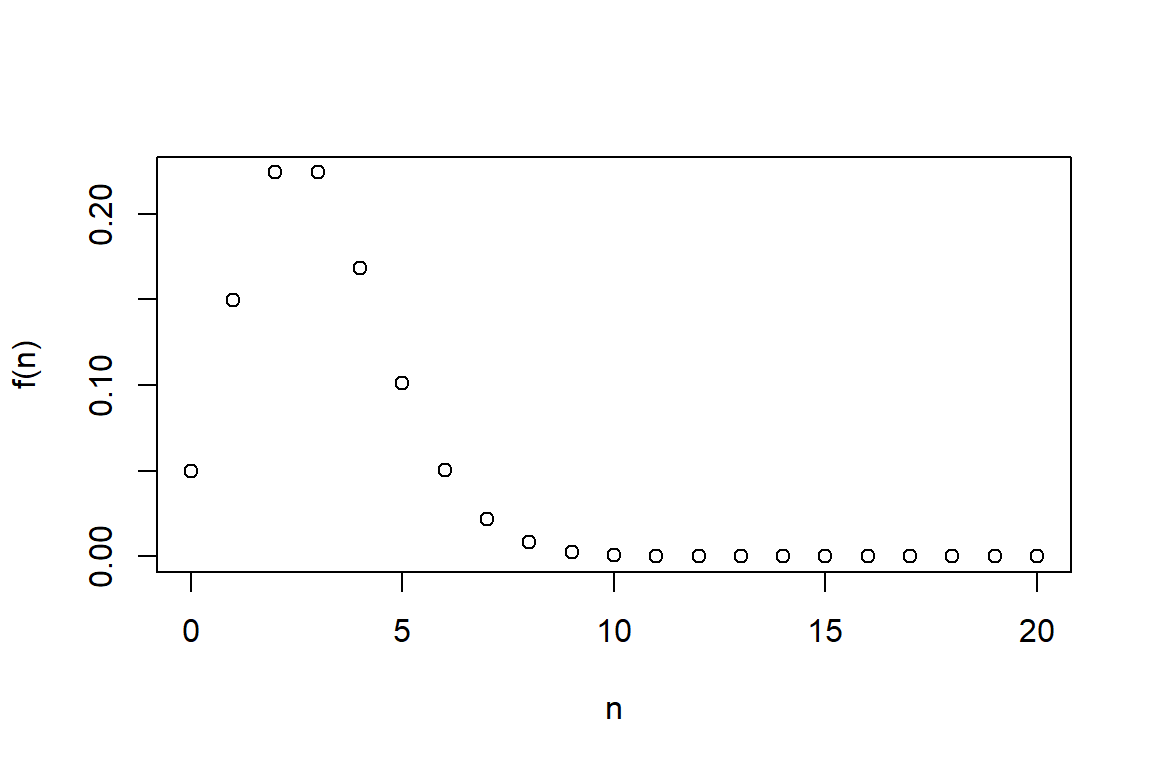
\includegraphics{R_for_Loss_Data_Analytics_files/figure-latex/unnamed-chunk-13-1} \end{center}

A few quick notes on these commands.

\begin{itemize}
\tightlist
\item
  The assigment operator \texttt{\textless{}-} is analogous to an equal
  sign in mathematics. The command \texttt{lambda\ \textless{}-\ 3}
  means to give a value of ``3'' to quantity \emph{lambda}.
\item
  \texttt{seq} is short-hand for sequence.
\item
  \texttt{dpois} is a built-in command in \textbf{R} for generating the
  ``density'' (actually the mass) function of the Poisson distribution.
  Use the online help (\texttt{help("dpois")}) to learn more about this
  function.
\item
  The open paren \texttt{(}, close paren \texttt{)} tells \textbf{R} to
  display the output of a calculation to the screen.
\item
  \texttt{plot} is a very handy command for displaying results
  graphically.
\end{itemize}

\subsubsection{(Cumulative) Probability Distribution Function
(cdf)}\label{cumulative-probability-distribution-function-cdf}

\begin{Shaded}
\begin{Highlighting}[]
\CommentTok{# Get the cumulative distribution function using "ppois"}
\NormalTok{( Fn <-}\StringTok{ }\KeywordTok{ppois}\NormalTok{(N, lambda) )}
\end{Highlighting}
\end{Shaded}

\begin{verbatim}
 [1] 0.04978707 0.19914827 0.42319008 0.64723189 0.81526324 0.91608206
 [7] 0.96649146 0.98809550 0.99619701 0.99889751 0.99970766 0.99992861
[13] 0.99998385 0.99999660 0.99999933 0.99999988 0.99999998 1.00000000
[19] 1.00000000 1.00000000 1.00000000
\end{verbatim}

\begin{Shaded}
\begin{Highlighting}[]
\CommentTok{# Visualize the cumulative distribution function}
\KeywordTok{plot}\NormalTok{(N, Fn, }\DataTypeTok{xlab =} \StringTok{"n"}\NormalTok{, }\DataTypeTok{ylab =} \StringTok{"F(n)"}\NormalTok{) }\CommentTok{# cdf}
\end{Highlighting}
\end{Shaded}

\begin{center}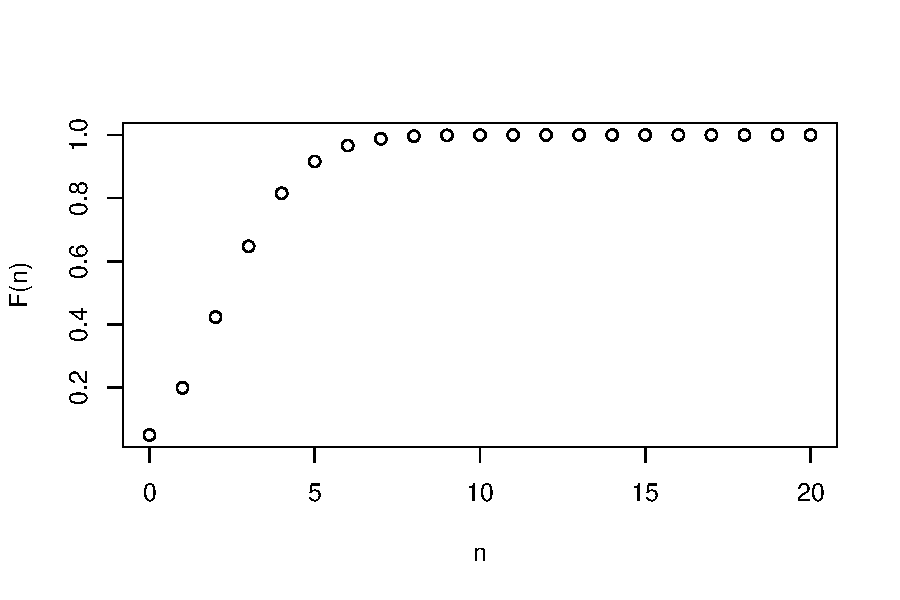
\includegraphics{R_for_Loss_Data_Analytics_files/figure-latex/unnamed-chunk-14-1} \end{center}

\subsection{Negative Binomial
Distribution}\label{negative-binomial-distribution}

This section shows how to compute and graph probability mass and
distribution functions for the negative binomial distribution. You will
also learn how to plot two functions on the same graph.

\subsubsection{Probability Mass Function
(pmf)}\label{probability-mass-function-pmf-1}

\begin{Shaded}
\begin{Highlighting}[]
\NormalTok{alpha <-}\StringTok{ }\DecValTok{3}
\NormalTok{theta <-}\StringTok{ }\DecValTok{2}
\NormalTok{prob <-}\StringTok{ }\DecValTok{1} \OperatorTok{/}\StringTok{ }\NormalTok{(}\DecValTok{1} \OperatorTok{+}\StringTok{ }\NormalTok{theta)}
\NormalTok{N <-}\StringTok{ }\KeywordTok{seq}\NormalTok{(}\DecValTok{0}\NormalTok{, }\DecValTok{30}\NormalTok{, }\DecValTok{1}\NormalTok{)}
\CommentTok{# Get the probability mass function using "dnbinom"}
\NormalTok{( fn <-}\StringTok{ }\KeywordTok{dnbinom}\NormalTok{(N, alpha, prob) )}
\end{Highlighting}
\end{Shaded}

\begin{verbatim}
 [1] 3.703704e-02 7.407407e-02 9.876543e-02 1.097394e-01 1.097394e-01
 [6] 1.024234e-01 9.104303e-02 7.803688e-02 6.503074e-02 5.298801e-02
[11] 4.239041e-02 3.339850e-02 2.597661e-02 1.998201e-02 1.522439e-02
[16] 1.150287e-02 8.627153e-03 6.428075e-03 4.761537e-03 3.508501e-03
[21] 2.572901e-03 1.878626e-03 1.366273e-03 9.900532e-04 7.150384e-04
[26] 5.148277e-04 3.696199e-04 2.646661e-04 1.890472e-04 1.347233e-04
[31] 9.580323e-05
\end{verbatim}

\begin{Shaded}
\begin{Highlighting}[]
\CommentTok{# Visualize the probability mass function}
\KeywordTok{plot}\NormalTok{(N, fn, }\DataTypeTok{xlab =} \StringTok{"n"}\NormalTok{, }\DataTypeTok{ylab =} \StringTok{"f(n)"}\NormalTok{) }\CommentTok{# pmf}
\end{Highlighting}
\end{Shaded}

\begin{center}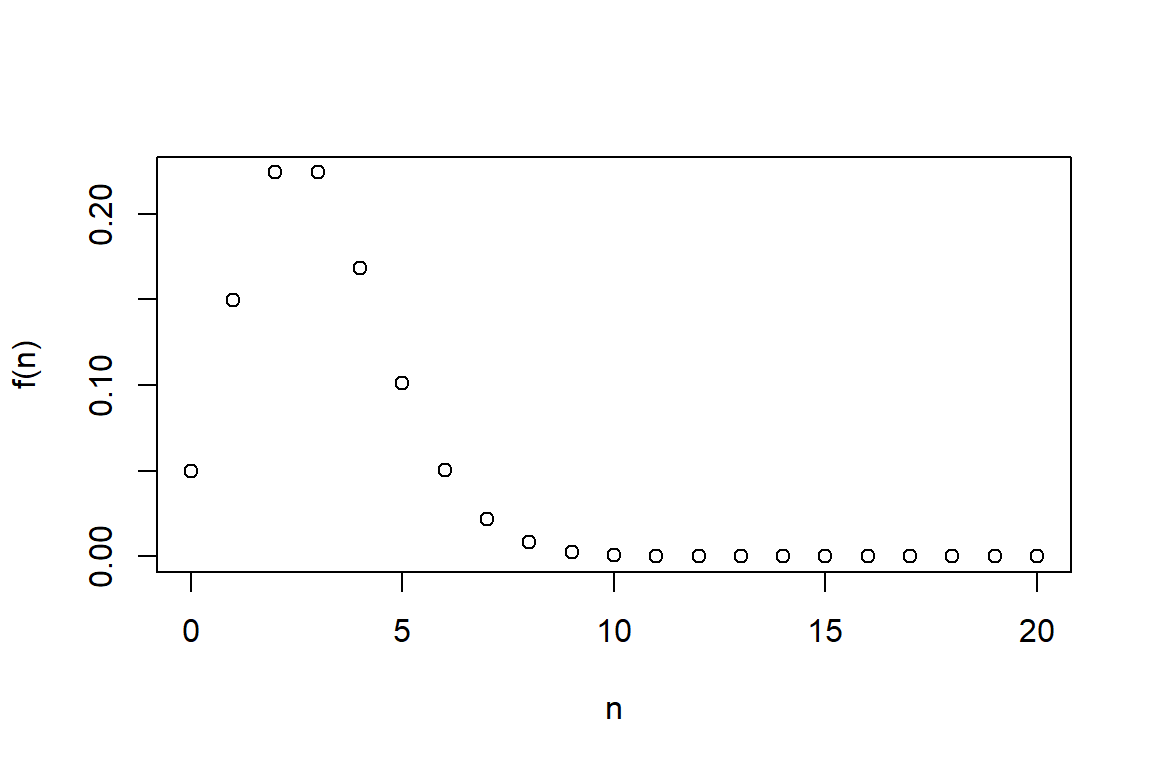
\includegraphics{R_for_Loss_Data_Analytics_files/figure-latex/unnamed-chunk-15-1} \end{center}

\paragraph{Plot Two Functions on The Same
Graph}\label{plot-two-functions-on-the-same-graph}

\begin{Shaded}
\begin{Highlighting}[]
\CommentTok{# Plot different negative binomial distributions on the same figure}
\NormalTok{alpha_}\DecValTok{1}\NormalTok{ <-}\StringTok{ }\DecValTok{3}
\NormalTok{alpha_}\DecValTok{2}\NormalTok{ <-}\StringTok{ }\DecValTok{5}
\NormalTok{theta <-}\StringTok{ }\DecValTok{2}
\NormalTok{prob <-}\StringTok{ }\DecValTok{1} \OperatorTok{/}\StringTok{ }\NormalTok{(}\DecValTok{1} \OperatorTok{+}\StringTok{ }\NormalTok{theta)}
\NormalTok{fn_}\DecValTok{1}\NormalTok{ <-}\StringTok{ }\KeywordTok{dnbinom}\NormalTok{(N, alpha_}\DecValTok{1}\NormalTok{, prob)}
\NormalTok{fn_}\DecValTok{2}\NormalTok{ <-}\StringTok{ }\KeywordTok{dnbinom}\NormalTok{(N, alpha_}\DecValTok{2}\NormalTok{, prob)}
\KeywordTok{plot}\NormalTok{(N, fn_}\DecValTok{1}\NormalTok{, }\DataTypeTok{xlab =} \StringTok{"n"}\NormalTok{, }\DataTypeTok{ylab =} \StringTok{"f(n)"}\NormalTok{)}
\KeywordTok{lines}\NormalTok{(N, fn_}\DecValTok{2}\NormalTok{, }\DataTypeTok{col =} \StringTok{"red"}\NormalTok{, }\DataTypeTok{type =} \StringTok{"p"}\NormalTok{)}
\end{Highlighting}
\end{Shaded}

\begin{center}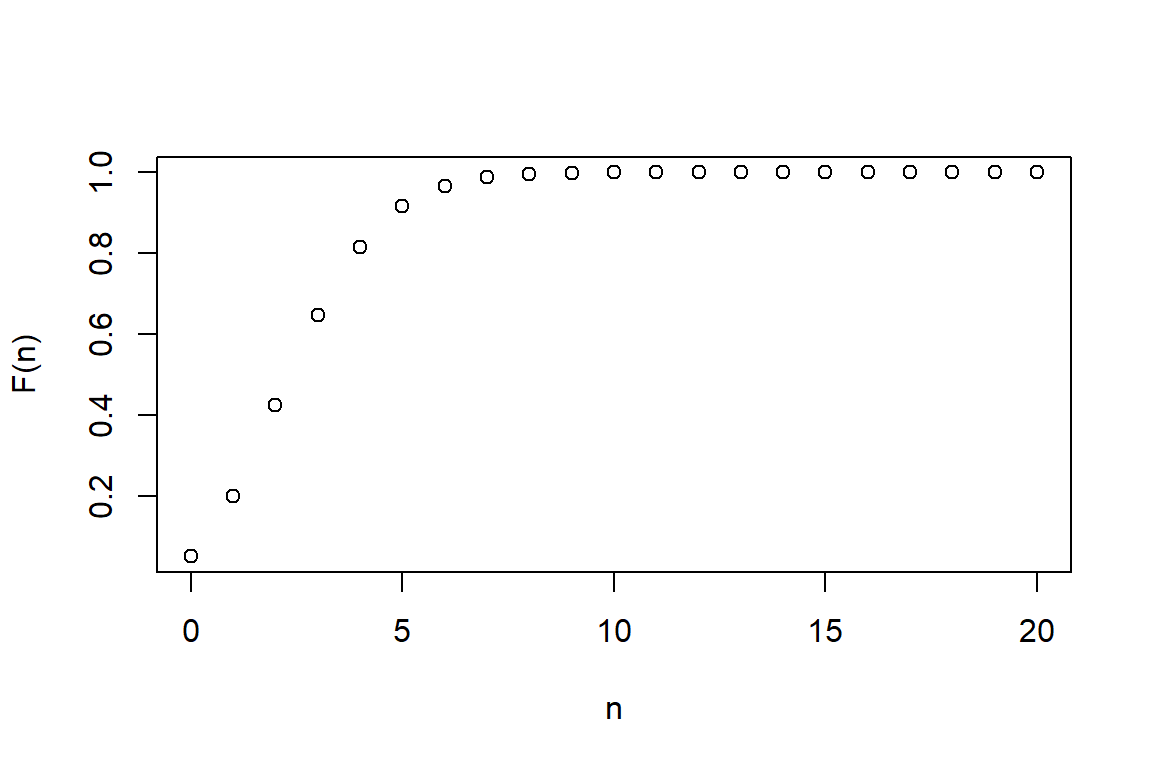
\includegraphics{R_for_Loss_Data_Analytics_files/figure-latex/unnamed-chunk-16-1} \end{center}

A couple notes on these commands:

\begin{itemize}
\tightlist
\item
  You can enter more than one command on a line; separate them using the
  \texttt{;} semi-colon.
\item
  \texttt{lines} is very handy for superimposing one graph on another.
\item
  When making complex graphs with more than one function, consider using
  different colors. The \texttt{col\ =\ "red"} tells \textbf{R} to use
  the color red when plotting symbols.
\end{itemize}

\subsubsection{(Cumulative) Probability Distribution Function
(cdf)}\label{cumulative-probability-distribution-function-cdf-1}

\begin{Shaded}
\begin{Highlighting}[]
\CommentTok{# Get the distribution function using "pnbinom"}
\NormalTok{( Fn <-}\StringTok{ }\KeywordTok{pnbinom}\NormalTok{(N, alpha, prob) )}
\end{Highlighting}
\end{Shaded}

\begin{verbatim}
 [1] 0.03703704 0.11111111 0.20987654 0.31961591 0.42935528 0.53177869
 [7] 0.62282172 0.70085861 0.76588935 0.81887735 0.86126776 0.89466626
[13] 0.92064288 0.94062489 0.95584927 0.96735214 0.97597930 0.98240737
[19] 0.98716891 0.99067741 0.99325031 0.99512894 0.99649521 0.99748526
[25] 0.99820030 0.99871513 0.99908475 0.99934942 0.99953846 0.99967319
[31] 0.99976899
\end{verbatim}

\begin{Shaded}
\begin{Highlighting}[]
\KeywordTok{plot}\NormalTok{(N, Fn, }\DataTypeTok{xlab =} \StringTok{"n"}\NormalTok{, }\DataTypeTok{ylab =} \StringTok{"F(n)"}\NormalTok{)  }\CommentTok{# cdf}
\end{Highlighting}
\end{Shaded}

\begin{center}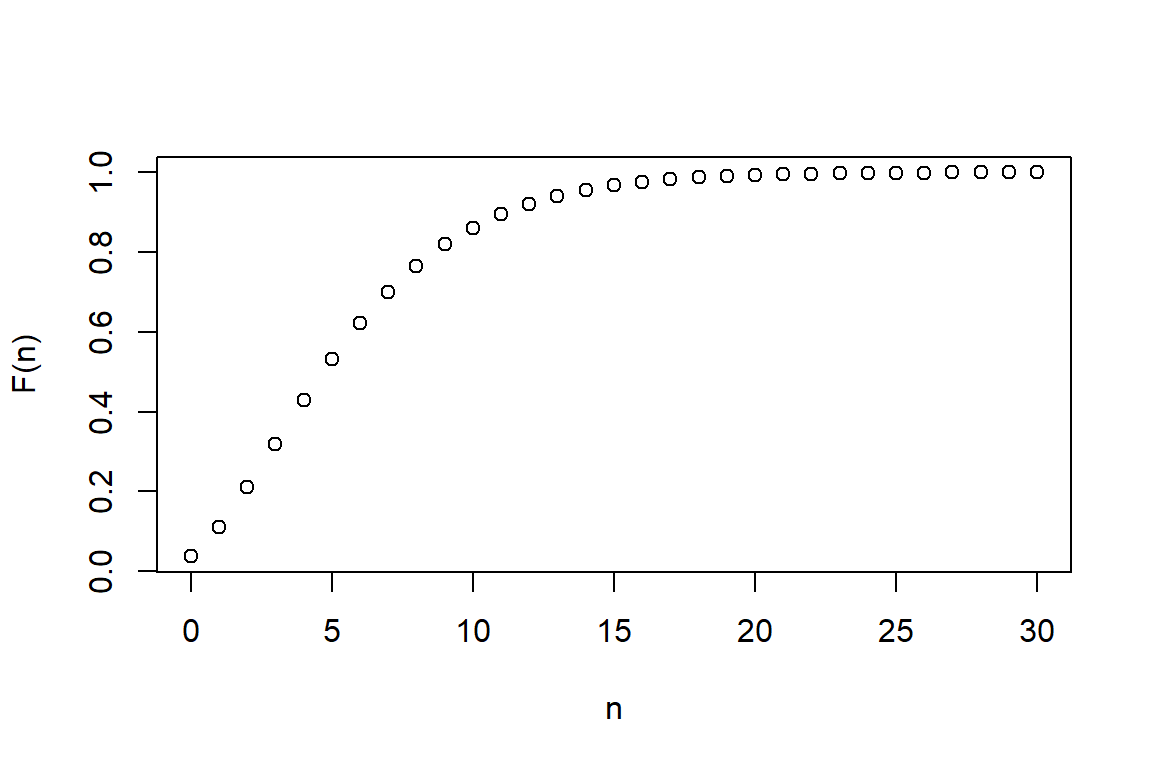
\includegraphics{R_for_Loss_Data_Analytics_files/figure-latex/unnamed-chunk-17-1} \end{center}

\subsection{Binomial Distribution}\label{binomial-distribution}

This section shows how to compute and graph probability mass and
distribution functions for the binomial distribution.

\subsubsection{Probability Mass Function
(pmf)}\label{probability-mass-function-pmf-2}

\begin{Shaded}
\begin{Highlighting}[]
\CommentTok{# Plot different binomial distributions on the same figure}
\NormalTok{size <-}\StringTok{ }\DecValTok{30}
\NormalTok{prob <-}\StringTok{ }\FloatTok{0.6}
\NormalTok{N <-}\StringTok{ }\KeywordTok{seq}\NormalTok{(}\DecValTok{0}\NormalTok{, }\DecValTok{30}\NormalTok{, }\DecValTok{1}\NormalTok{)}
\NormalTok{fn <-}\StringTok{ }\KeywordTok{dbinom}\NormalTok{(N, size, prob)}
\KeywordTok{plot}\NormalTok{(N, fn, }\DataTypeTok{xlab =} \StringTok{"n"}\NormalTok{, }\DataTypeTok{ylab =} \StringTok{"f(n)"}\NormalTok{)  }\CommentTok{# pdf}
\NormalTok{fn2 <-}\StringTok{ }\KeywordTok{dbinom}\NormalTok{(N, size, }\FloatTok{0.7}\NormalTok{)}
\KeywordTok{lines}\NormalTok{(N, fn2, }\DataTypeTok{col =} \StringTok{"red"}\NormalTok{, }\DataTypeTok{type =} \StringTok{"p"}\NormalTok{)}
\end{Highlighting}
\end{Shaded}

\begin{center}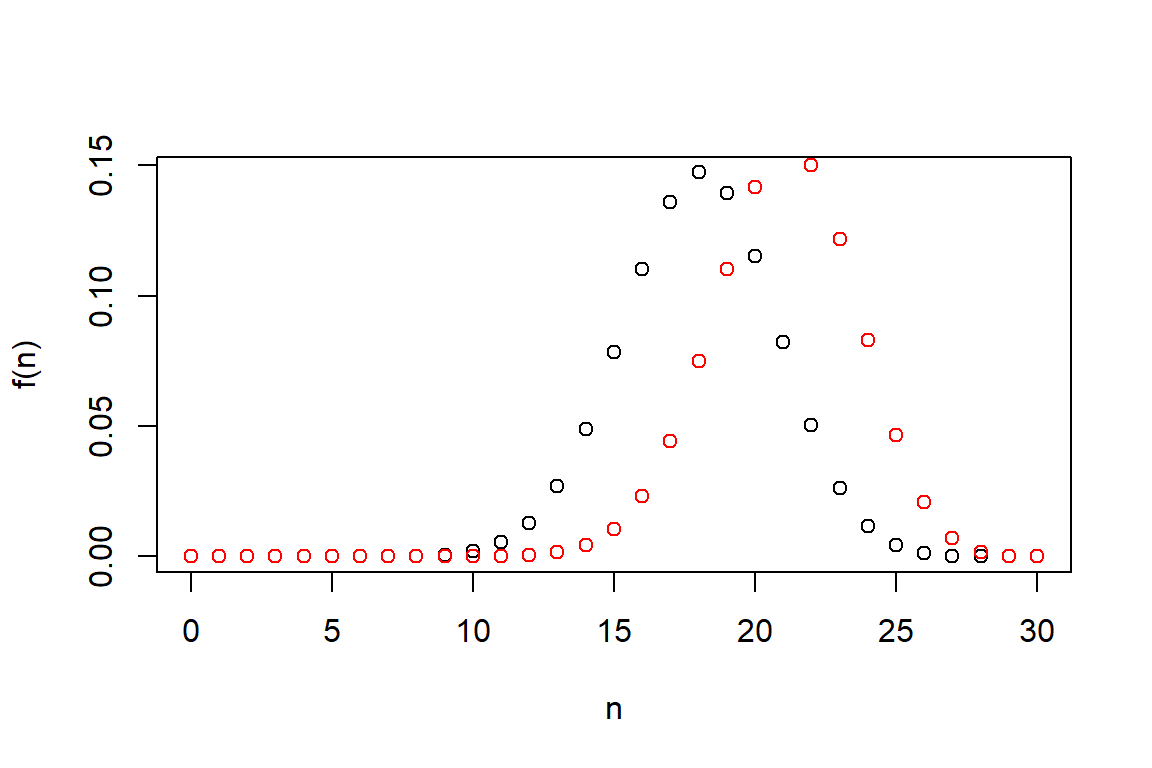
\includegraphics{R_for_Loss_Data_Analytics_files/figure-latex/unnamed-chunk-18-1} \end{center}

\subsubsection{(Cumulative) Probability Distribution Function
(cdf)}\label{cumulative-probability-distribution-function-cdf-2}

\begin{Shaded}
\begin{Highlighting}[]
\CommentTok{# Get the distribution function using "pbinom"}
\NormalTok{( Fn <-}\StringTok{ }\KeywordTok{pbinom}\NormalTok{(N, size, prob) )}
\end{Highlighting}
\end{Shaded}

\begin{verbatim}
 [1] 1.152922e-12 5.303439e-11 1.181456e-09 1.697936e-08 1.769332e-07
 [6] 1.424573e-06 9.222321e-06 4.932503e-05 2.222679e-04 8.563920e-04
[11] 2.853883e-03 8.301584e-03 2.123988e-02 4.811171e-02 9.705684e-02
[16] 1.753691e-01 2.854956e-01 4.215343e-01 5.689095e-01 7.085281e-01
[21] 8.237135e-01 9.059888e-01 9.564759e-01 9.828170e-01 9.943412e-01
[26] 9.984899e-01 9.996867e-01 9.999526e-01 9.999954e-01 9.999998e-01
[31] 1.000000e+00
\end{verbatim}

\begin{Shaded}
\begin{Highlighting}[]
\KeywordTok{plot}\NormalTok{(N, Fn, }\DataTypeTok{xlab =} \StringTok{"n"}\NormalTok{, }\DataTypeTok{ylab =} \StringTok{"F(n)"}\NormalTok{)  }\CommentTok{# cdf}
\end{Highlighting}
\end{Shaded}

\begin{center}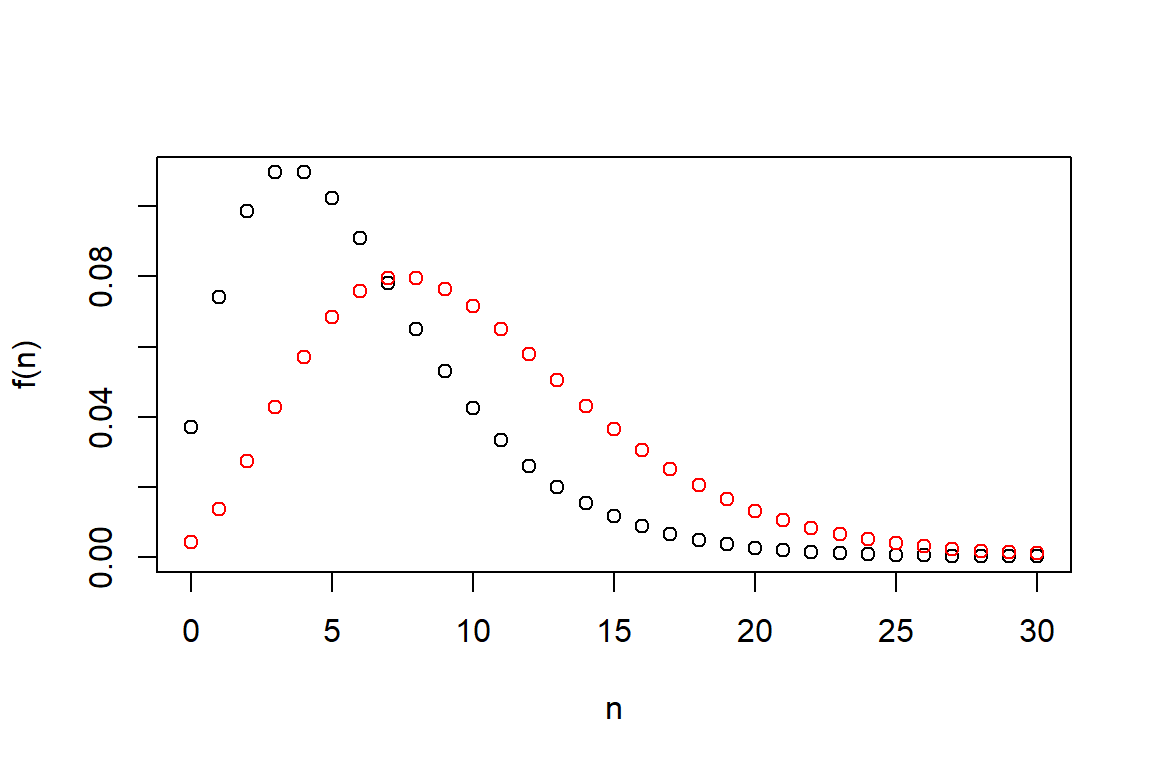
\includegraphics{R_for_Loss_Data_Analytics_files/figure-latex/unnamed-chunk-19-1} \end{center}

\section{\texorpdfstring{(\emph{a},\emph{b},0) Class of
Distributions}{(a,b,0) Class of Distributions}}\label{ab0-class-of-distributions}

This section shows how to compute recursively a distribution in the
(\emph{a},\emph{b},0) class. The specific example is a Poisson. However,
by changing values of \emph{a} and \emph{b}, you can use the same
recursion for negative binomial and binomial, the other two members of
the (\emph{a},\emph{b},0) class.

\begin{Shaded}
\begin{Highlighting}[]
\NormalTok{lambda <-}\StringTok{ }\DecValTok{3}
\NormalTok{a <-}\StringTok{ }\DecValTok{0}
\NormalTok{b <-}\StringTok{ }\NormalTok{lambda}
\CommentTok{# This loop calculates the (a,b,0) recursive probabilities for the Poisson distribution}
\NormalTok{p <-}\StringTok{ }\KeywordTok{rep}\NormalTok{(}\DecValTok{0}\NormalTok{, }\DecValTok{20}\NormalTok{)}
\CommentTok{# Get the probability at n = 0 to start the recursive formula }
\NormalTok{p[}\DecValTok{1}\NormalTok{] <-}\StringTok{ }\KeywordTok{exp}\NormalTok{(}\OperatorTok{-}\NormalTok{lambda)}
\ControlFlowTok{for}\NormalTok{ (i }\ControlFlowTok{in} \DecValTok{1}\OperatorTok{:}\DecValTok{19}\NormalTok{)}
\NormalTok{  \{}
\NormalTok{  p[i}\OperatorTok{+}\DecValTok{1}\NormalTok{] <-}\StringTok{ }\NormalTok{(a }\OperatorTok{+}\StringTok{ }\NormalTok{b }\OperatorTok{/}\StringTok{ }\NormalTok{i) }\OperatorTok{*}\StringTok{ }\NormalTok{p[i]  }\CommentTok{# Probability of i-th element using the ab0 formula}
\NormalTok{  \}}
\NormalTok{p}
\end{Highlighting}
\end{Shaded}

\begin{verbatim}
 [1] 4.978707e-02 1.493612e-01 2.240418e-01 2.240418e-01 1.680314e-01
 [6] 1.008188e-01 5.040941e-02 2.160403e-02 8.101512e-03 2.700504e-03
[11] 8.101512e-04 2.209503e-04 5.523758e-05 1.274713e-05 2.731529e-06
[16] 5.463057e-07 1.024323e-07 1.807629e-08 3.012715e-09 4.756919e-10
\end{verbatim}

\begin{Shaded}
\begin{Highlighting}[]
\CommentTok{# Check using the "dpois" command}
\KeywordTok{dpois}\NormalTok{(}\KeywordTok{seq}\NormalTok{(}\DecValTok{0}\NormalTok{, }\DecValTok{20}\NormalTok{, }\DecValTok{1}\NormalTok{), }\DataTypeTok{lambda =} \DecValTok{3}\NormalTok{)}
\end{Highlighting}
\end{Shaded}

\begin{verbatim}
 [1] 4.978707e-02 1.493612e-01 2.240418e-01 2.240418e-01 1.680314e-01
 [6] 1.008188e-01 5.040941e-02 2.160403e-02 8.101512e-03 2.700504e-03
[11] 8.101512e-04 2.209503e-04 5.523758e-05 1.274713e-05 2.731529e-06
[16] 5.463057e-07 1.024323e-07 1.807629e-08 3.012715e-09 4.756919e-10
[21] 7.135379e-11
\end{verbatim}

A couple notes on these commands.

\begin{itemize}
\tightlist
\item
  There are many basic math commands in \textbf{R} such as \texttt{exp}
  for exponentials.
\item
  This demo illustrates the use of the \texttt{for} loop, one of many
  ways of doing recursive calculations.
\end{itemize}

\section{Estimating Frequency
Distributions}\label{estimating-frequency-distributions}

\subsection{Singapore Data}\label{singapore-data}

This section loads the \texttt{SingaporeAuto.csv} dataset and checks the
names of variables and the dimensions of the data. To have a glimpse at
the data, the first 8 observations are listed.

\begin{Shaded}
\begin{Highlighting}[]
\NormalTok{Singapore <-}\StringTok{ }\KeywordTok{read.csv}\NormalTok{(}\StringTok{"Data/SingaporeAuto.csv"}\NormalTok{, }\DataTypeTok{quote =} \StringTok{""}\NormalTok{, }\DataTypeTok{header =} \OtherTok{TRUE}\NormalTok{)}
\CommentTok{# Check the names, dimensions in the file and list the first 8 observations ;}
\KeywordTok{names}\NormalTok{(Singapore)}
\end{Highlighting}
\end{Shaded}

\begin{verbatim}
 [1] "SexInsured"  "Female"      "VehicleType" "PC"          "Clm_Count"  
 [6] "Exp_weights" "LNWEIGHT"    "NCD"         "AgeCat"      "AutoAge0"   
[11] "AutoAge1"    "AutoAge2"    "AutoAge"     "VAgeCat"     "VAgecat1"   
\end{verbatim}

\begin{Shaded}
\begin{Highlighting}[]
\KeywordTok{dim}\NormalTok{(Singapore)  }\CommentTok{# check number of observations and variables in the data}
\end{Highlighting}
\end{Shaded}

\begin{verbatim}
[1] 7483   15
\end{verbatim}

\begin{Shaded}
\begin{Highlighting}[]
\NormalTok{Singapore[}\DecValTok{1}\OperatorTok{:}\DecValTok{4}\NormalTok{, ]  }\CommentTok{# list the first 4 observations}
\end{Highlighting}
\end{Shaded}

\begin{verbatim}
  SexInsured Female VehicleType PC Clm_Count Exp_weights    LNWEIGHT NCD
1          U      0           T  0         0   0.6680356 -0.40341383  30
2          U      0           T  0         0   0.5667351 -0.56786326  30
3          U      0           T  0         0   0.5037645 -0.68564629  30
4          U      0           T  0         0   0.9144422 -0.08944106  20
  AgeCat AutoAge0 AutoAge1 AutoAge2 AutoAge VAgeCat VAgecat1
1      0        0        0        0       0       0        2
2      0        0        0        0       0       0        2
3      0        0        0        0       0       0        2
4      0        0        0        0       0       0        2
\end{verbatim}

\begin{Shaded}
\begin{Highlighting}[]
\KeywordTok{attach}\NormalTok{(Singapore)  }\CommentTok{# attach dataset}
\end{Highlighting}
\end{Shaded}

A few quick notes on these commands:

\begin{itemize}
\tightlist
\item
  The \texttt{names()}function is used to get or assign names of an
  object. In this illustration, it was used to get the variables names.
\item
  The \texttt{dim()} function is used to retrieve or set the dimensions
  of an object.
\item
  When you attach a dataset using the \texttt{attach()} function,
  variable names in the database can be accessed by simply giving their
  names.
\end{itemize}

\subsection{Claim Frequency
Distribution}\label{claim-frequency-distribution-1}

The table below gives the distribution of observed claims frequency. The
\texttt{Clm\_Count} variable is the number of automobile accidents per
policyholder.

\begin{Shaded}
\begin{Highlighting}[]
\KeywordTok{table}\NormalTok{(Clm_Count) }
\end{Highlighting}
\end{Shaded}

\begin{verbatim}
Clm_Count
   0    1    2    3 
6996  455   28    4 
\end{verbatim}

\begin{Shaded}
\begin{Highlighting}[]
\NormalTok{( n <-}\StringTok{ }\KeywordTok{length}\NormalTok{(Clm_Count) )  }\CommentTok{# number of insurance policies }
\end{Highlighting}
\end{Shaded}

\begin{verbatim}
[1] 7483
\end{verbatim}

\subsection{Visualize The Loglikelihood
Function}\label{visualize-the-loglikelihood-function}

Before maximizing, let us start by visualizing the logarithmic
likelihood function. We will fit the claim counts for the Singapore data
to the Poisson model. As an illustration, first assume that
\(\lambda = 0.5\). The claim count, likelihood, and its logarithmic
version, for five observations is

\begin{Shaded}
\begin{Highlighting}[]
\CommentTok{# Five typical observations}
\NormalTok{Clm_Count[}\DecValTok{2245}\OperatorTok{:}\DecValTok{2249}\NormalTok{]}
\end{Highlighting}
\end{Shaded}

\begin{verbatim}
[1] 3 0 1 0 3
\end{verbatim}

\begin{Shaded}
\begin{Highlighting}[]
\CommentTok{# Probabilities}
\KeywordTok{dpois}\NormalTok{(Clm_Count[}\DecValTok{2245}\OperatorTok{:}\DecValTok{2249}\NormalTok{], }\DataTypeTok{lambda =} \FloatTok{0.5}\NormalTok{)}
\end{Highlighting}
\end{Shaded}

\begin{verbatim}
[1] 0.01263606 0.60653066 0.30326533 0.60653066 0.01263606
\end{verbatim}

\begin{Shaded}
\begin{Highlighting}[]
\CommentTok{# Logarithmic probabilities}
\KeywordTok{log}\NormalTok{(}\KeywordTok{dpois}\NormalTok{(Clm_Count[}\DecValTok{2245}\OperatorTok{:}\DecValTok{2249}\NormalTok{], }\DataTypeTok{lambda =} \FloatTok{0.5}\NormalTok{))}
\end{Highlighting}
\end{Shaded}

\begin{verbatim}
[1] -4.371201 -0.500000 -1.193147 -0.500000 -4.371201
\end{verbatim}

By hand, you can check that the sum of log likelihoods for these five
observations is -10.9355492. In the same way, the sum of all 7483
observations is

\begin{Shaded}
\begin{Highlighting}[]
\KeywordTok{sum}\NormalTok{(}\KeywordTok{log}\NormalTok{(}\KeywordTok{dpois}\NormalTok{(Clm_Count, }\DataTypeTok{lambda =} \FloatTok{0.5}\NormalTok{)))}
\end{Highlighting}
\end{Shaded}

\begin{verbatim}
[1] -4130.591
\end{verbatim}

Of course, this is only for the choice \(\lambda = 0.5\). The following
code defines the log likelihood to be a function of \(\lambda\) and
plots the function for several choices of \(\lambda\):

\begin{Shaded}
\begin{Highlighting}[]
\NormalTok{loglikPois <-}\StringTok{ }\ControlFlowTok{function}\NormalTok{ (parms)\{ }
\CommentTok{# Defines the Poisson loglikelihood function  }
\NormalTok{  lambda =}\StringTok{ }\NormalTok{parms[}\DecValTok{1}\NormalTok{]}
\NormalTok{  llk <-}\StringTok{ }\KeywordTok{sum}\NormalTok{(}\KeywordTok{log}\NormalTok{(}\KeywordTok{dpois}\NormalTok{(Clm_Count, lambda)))}
\NormalTok{  llk}
\NormalTok{\} }
\NormalTok{lambdax <-}\StringTok{ }\KeywordTok{seq}\NormalTok{(}\DecValTok{0}\NormalTok{, .}\DecValTok{2}\NormalTok{, .}\DecValTok{01}\NormalTok{)}
\NormalTok{loglike <-}\StringTok{ }\DecValTok{0} \OperatorTok{*}\StringTok{ }\NormalTok{lambdax}
\ControlFlowTok{for}\NormalTok{ (i }\ControlFlowTok{in} \DecValTok{1}\OperatorTok{:}\KeywordTok{length}\NormalTok{(lambdax)) }
\NormalTok{  \{}
\NormalTok{  loglike[i] <-}\StringTok{ }\KeywordTok{loglikPois}\NormalTok{(lambdax[i])}
\NormalTok{\}}
\KeywordTok{plot}\NormalTok{(lambdax, loglike)}
\end{Highlighting}
\end{Shaded}

\begin{center}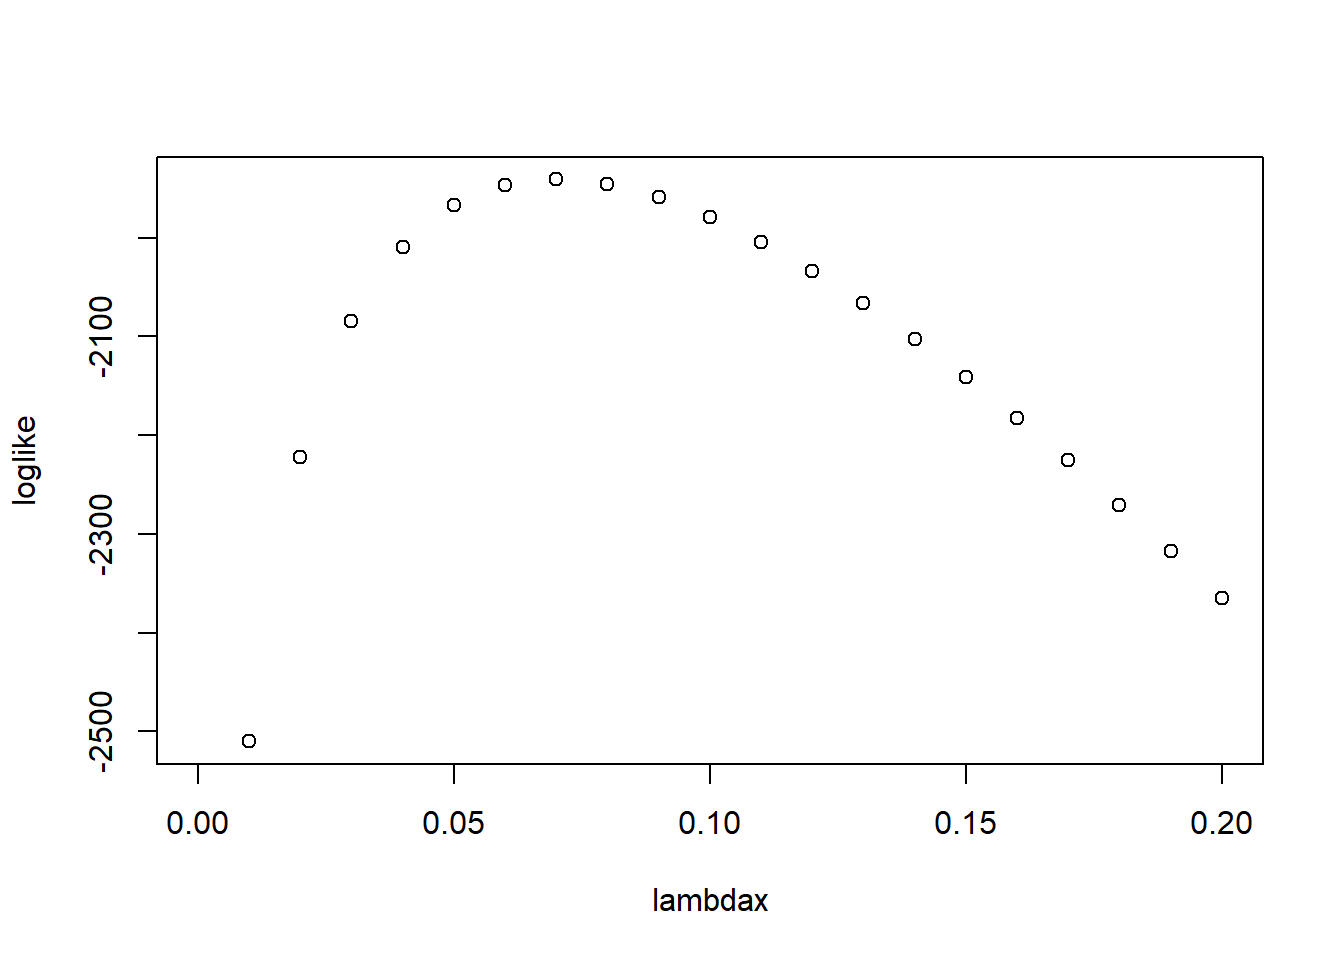
\includegraphics{R_for_Loss_Data_Analytics_files/figure-latex/unnamed-chunk-25-1} \end{center}

If we had to guess, from this plot we might say that the maximum value
of the log likelihood was around 0.07.

\subsection{The Maximum Likelihood Estimate of Poisson
Distribution}\label{the-maximum-likelihood-estimate-of-poisson-distribution}

From calculus, we know that the maximum likelihood estimator
(\emph{mle}) of the Poisson distribution parameter equals the average
claim count. For our data, this is

\begin{Shaded}
\begin{Highlighting}[]
\KeywordTok{mean}\NormalTok{(Clm_Count)}
\end{Highlighting}
\end{Shaded}

\begin{verbatim}
[1] 0.06989175
\end{verbatim}

As an alternative, let us use an optimization routine \texttt{nlminb}.
Most optimization routines try to minimize functions instead of maximize
them, so we first define the \emph{negative} loglikelihood function.

\begin{Shaded}
\begin{Highlighting}[]
\NormalTok{negloglikPois <-}\StringTok{ }\ControlFlowTok{function}\NormalTok{ (parms)\{}
\CommentTok{# Defines the (negative) Poisson loglikelihood function  }
\NormalTok{  lambda <-}\StringTok{ }\NormalTok{parms[}\DecValTok{1}\NormalTok{]}
\NormalTok{  llk <-}\StringTok{ }\OperatorTok{-}\KeywordTok{sum}\NormalTok{(}\KeywordTok{log}\NormalTok{(}\KeywordTok{dpois}\NormalTok{(Clm_Count, lambda)))}
\NormalTok{  llk}
\NormalTok{\} }
\NormalTok{ini.Pois <-}\StringTok{ }\DecValTok{1} 
\NormalTok{zop.Pois <-}\StringTok{ }\KeywordTok{nlminb}\NormalTok{(ini.Pois, negloglikPois, }\DataTypeTok{lower =} \KeywordTok{c}\NormalTok{(}\FloatTok{1e-6}\NormalTok{), }\DataTypeTok{upper =} \KeywordTok{c}\NormalTok{(}\OtherTok{Inf}\NormalTok{))}
\KeywordTok{print}\NormalTok{(zop.Pois)  }\CommentTok{# In output, $par = MLE of lambda, $objective = - loglikelihood value}
\end{Highlighting}
\end{Shaded}

\begin{verbatim}
$par
[1] 0.06989175

$objective
[1] 1941.178

$convergence
[1] 0

$iterations
[1] 17

$evaluations
function gradient 
      23       20 

$message
[1] "relative convergence (4)"
\end{verbatim}

So, the maximum likelihood estimate, \texttt{zop.Pois\$par\ =} 0.0698918
is exactly the same as the value that we got by hand.

Because actuarial analysts calculate Poisson mle's so regularly, here is
another way of doing the calculation using the \texttt{glm},
\emph{generalized linear model}, package.

\begin{Shaded}
\begin{Highlighting}[]
\NormalTok{count_poisson1 <-}\StringTok{ }\KeywordTok{glm}\NormalTok{(Clm_Count }\OperatorTok{~}\StringTok{ }\DecValTok{1}\NormalTok{, }\KeywordTok{poisson}\NormalTok{(}\DataTypeTok{link =}\NormalTok{ log))}
\KeywordTok{summary}\NormalTok{(count_poisson1)}
\end{Highlighting}
\end{Shaded}

\begin{verbatim}

Call:
glm(formula = Clm_Count ~ 1, family = poisson(link = log))

Deviance Residuals: 
    Min       1Q   Median       3Q      Max  
-0.3739  -0.3739  -0.3739  -0.3739   4.0861  

Coefficients:
            Estimate Std. Error z value Pr(>|z|)    
(Intercept) -2.66081    0.04373  -60.85   <2e-16 ***
---
Signif. codes:  0 '***' 0.001 '**' 0.01 '*' 0.05 '.' 0.1 ' ' 1

(Dispersion parameter for poisson family taken to be 1)

    Null deviance: 2887.2  on 7482  degrees of freedom
Residual deviance: 2887.2  on 7482  degrees of freedom
AIC: 3884.4

Number of Fisher Scoring iterations: 6
\end{verbatim}

\begin{Shaded}
\begin{Highlighting}[]
\NormalTok{( lambda_hat <-}\StringTok{ }\KeywordTok{exp}\NormalTok{(count_poisson1}\OperatorTok{$}\NormalTok{coefficients) )}
\end{Highlighting}
\end{Shaded}

\begin{verbatim}
(Intercept) 
 0.06989175 
\end{verbatim}

A few quick notes on these commands and results:

\begin{itemize}
\tightlist
\item
  The \texttt{glm()}function is used to fit generalized linear models.
  See \texttt{help(glm)} for other modeling options. In order to get the
  results we use the \texttt{summary()} function.
\item
  In the output, \texttt{call} reminds us what model we ran and what
  options were specified.
\item
  The \texttt{Deviance\ Residuals} shows the distribution of the
  deviance residuals for individual cases used in the model.
\item
  The next part of the output shows the coefficient (maximum likelihood
  estimate of \(\log(\lambda)\)), its standard error, the z-statistic
  and the associated p-value.
\item
  To get the estimated \(\lambda\) we take the \(\exp\)(coefficient)
  \texttt{lambda\_hat\ \textless{}-\ exp(count\_poisson1\$coefficients)}.
\end{itemize}

\subsection{The Maximum Likelihood Estimate of The Negative Binomial
Distribution}\label{the-maximum-likelihood-estimate-of-the-negative-binomial-distribution}

In the same way, here is code for determining the maximum likelihood
estimates for the negative binomial distribution.

\begin{Shaded}
\begin{Highlighting}[]
\NormalTok{dnb <-}\StringTok{ }\ControlFlowTok{function}\NormalTok{ (y, r, beta)\{}
\CommentTok{# Defines the (negative) negative binomial loglikelihood function  }
  \KeywordTok{gamma}\NormalTok{(y }\OperatorTok{+}\StringTok{ }\NormalTok{r) }\OperatorTok{/}\StringTok{ }\KeywordTok{gamma}\NormalTok{(r) }\OperatorTok{/}\StringTok{ }\KeywordTok{gamma}\NormalTok{(y }\OperatorTok{+}\StringTok{ }\DecValTok{1}\NormalTok{) }\OperatorTok{*}\StringTok{ }\NormalTok{(}\DecValTok{1} \OperatorTok{/}\StringTok{ }\NormalTok{(}\DecValTok{1} \OperatorTok{+}\StringTok{ }\NormalTok{beta))}\OperatorTok{^}\NormalTok{r }\OperatorTok{*}\StringTok{ }\NormalTok{(beta }\OperatorTok{/}\StringTok{ }\NormalTok{(}\DecValTok{1} \OperatorTok{+}\StringTok{ }\NormalTok{beta))}\OperatorTok{^}\NormalTok{y}
\NormalTok{\}}
\NormalTok{loglikNB <-}\StringTok{ }\ControlFlowTok{function}\NormalTok{ (parms)\{ }
\NormalTok{  r =}\StringTok{ }\NormalTok{parms[}\DecValTok{1}\NormalTok{]}
\NormalTok{  beta =}\StringTok{ }\NormalTok{parms[}\DecValTok{2}\NormalTok{]}
\NormalTok{  llk <-}\StringTok{ }\OperatorTok{-}\KeywordTok{sum}\NormalTok{(}\KeywordTok{log}\NormalTok{(}\KeywordTok{dnb}\NormalTok{(Clm_Count, r, beta)))}
\NormalTok{  llk}
\NormalTok{\} }

\NormalTok{ini.NB <-}\StringTok{ }\KeywordTok{c}\NormalTok{(}\DecValTok{1}\NormalTok{, }\DecValTok{1}\NormalTok{)}
\NormalTok{zop.NB <-}\StringTok{ }\KeywordTok{nlminb}\NormalTok{(ini.NB, loglikNB, }\DataTypeTok{lower =} \KeywordTok{c}\NormalTok{(}\FloatTok{1e-6}\NormalTok{, }\FloatTok{1e-6}\NormalTok{), }\DataTypeTok{upper =} \KeywordTok{c}\NormalTok{(}\OtherTok{Inf}\NormalTok{, }\OtherTok{Inf}\NormalTok{))}
\KeywordTok{print}\NormalTok{(zop.NB)  }\CommentTok{# In output, $par = (MLE of r, MLE of beta), $objective = - loglikelihood value}
\end{Highlighting}
\end{Shaded}

\begin{verbatim}
$par
[1] 0.87401622 0.07996624

$objective
[1] 1932.383

$convergence
[1] 0

$iterations
[1] 24

$evaluations
function gradient 
      30       60 

$message
[1] "relative convergence (4)"
\end{verbatim}

Two quick notes:

\begin{itemize}
\tightlist
\item
  There are two parameters for this distribution, so that calculation by
  hand is not a good alternative.
\item
  The maximum likelihood estimator of \emph{r}, 0.8740162, is not an
  integer.
\end{itemize}

\section{Goodness of Fit}\label{goodness-of-fit}

This section shows how to check the adequacy of the Poisson and negative
binomial models for the Singapore data.

First, note that the variance for the \emph{count} data is 0.0757079
which is greater than the mean value, 0.0698918. This suggests that the
negative binomial model is preferred to the Poisson model.

Second, we will compute the \emph{Pearson goodness-of-fit statistic}.

\subsection{Pearson Goodness-of-Fit
Statistic}\label{pearson-goodness-of-fit-statistic}

The table below gives the distribution of fitted claims frequency using
Poisson distribution \(n \times p_k\)

\begin{Shaded}
\begin{Highlighting}[]
\NormalTok{table_1p =}\StringTok{ }\KeywordTok{cbind}\NormalTok{(n }\OperatorTok{*}\StringTok{ }\NormalTok{(}\KeywordTok{dpois}\NormalTok{(}\DecValTok{0}\NormalTok{, lambda_hat)),}
\NormalTok{                 n }\OperatorTok{*}\StringTok{ }\NormalTok{(}\KeywordTok{dpois}\NormalTok{(}\DecValTok{1}\NormalTok{, lambda_hat)),}
\NormalTok{                 n }\OperatorTok{*}\StringTok{ }\NormalTok{(}\KeywordTok{dpois}\NormalTok{(}\DecValTok{2}\NormalTok{, lambda_hat)),}
\NormalTok{                 n }\OperatorTok{*}\StringTok{ }\NormalTok{(}\KeywordTok{dpois}\NormalTok{(}\DecValTok{3}\NormalTok{, lambda_hat)),}
\NormalTok{                 n }\OperatorTok{*}\StringTok{ }\NormalTok{(}\DecValTok{1} \OperatorTok{-}\StringTok{ }\KeywordTok{ppois}\NormalTok{(}\DecValTok{3}\NormalTok{, lambda_hat)))  }
\CommentTok{# or n * (1 - dpois(0,lambda_hat) - dpois(1, lambda_hat) -}
\CommentTok{# dpois(2, lambda_hat) - dpois(3, lambda_hat)))}
\NormalTok{actual <-}\StringTok{ }\KeywordTok{data.frame}\NormalTok{(}\KeywordTok{table}\NormalTok{(Clm_Count))[,}\DecValTok{2}\NormalTok{];}
\NormalTok{actual[}\DecValTok{5}\NormalTok{] <-}\StringTok{ }\DecValTok{0}  \CommentTok{# assign 0 to claim counts greater than or equal to 4 in observed data}

\NormalTok{table_2p <-}\StringTok{ }\KeywordTok{rbind}\NormalTok{(}\KeywordTok{c}\NormalTok{(}\DecValTok{0}\NormalTok{, }\DecValTok{1}\NormalTok{, }\DecValTok{2}\NormalTok{, }\DecValTok{3}\NormalTok{, }\StringTok{"4+"}\NormalTok{), actual, }\KeywordTok{round}\NormalTok{(table_1p, }\DataTypeTok{digits =} \DecValTok{2}\NormalTok{))}
\KeywordTok{rownames}\NormalTok{(table_2p) <-}\StringTok{ }\KeywordTok{c}\NormalTok{(}\StringTok{"Number"}\NormalTok{,}\StringTok{"Actual"}\NormalTok{, }\StringTok{"Estimated Using Poisson"}\NormalTok{)}
\NormalTok{table_2p}
\end{Highlighting}
\end{Shaded}

\begin{verbatim}
                        [,1]      [,2]     [,3]    [,4]  [,5]  
Number                  "0"       "1"      "2"     "3"   "4+"  
Actual                  "6996"    "455"    "28"    "4"   "0"   
Estimated Using Poisson "6977.86" "487.69" "17.04" "0.4" "0.01"
\end{verbatim}

For goodness of fit, consider Pearson's chi-square statistic below. The
degrees of freedom (\emph{df}) equals the number of cells minus one
minus the number of estimated parameters.

\begin{Shaded}
\begin{Highlighting}[]
\CommentTok{# PEARSON GOODNESS-OF-FIT STATISTIC}
\NormalTok{diff =}\StringTok{ }\NormalTok{actual }\OperatorTok{-}\StringTok{ }\NormalTok{table_1p}
\NormalTok{( Pearson_p <-}\StringTok{ }\KeywordTok{sum}\NormalTok{(diff }\OperatorTok{*}\StringTok{ }\NormalTok{diff }\OperatorTok{/}\StringTok{ }\NormalTok{table_1p) )}
\end{Highlighting}
\end{Shaded}

\begin{verbatim}
[1] 41.98438
\end{verbatim}

\begin{Shaded}
\begin{Highlighting}[]
\CommentTok{# p-value}
\DecValTok{1} \OperatorTok{-}\StringTok{ }\KeywordTok{pchisq}\NormalTok{(Pearson_p, }\DataTypeTok{df =} \DecValTok{5} \OperatorTok{-}\StringTok{ }\DecValTok{1} \OperatorTok{-}\StringTok{ }\DecValTok{1}\NormalTok{)}
\end{Highlighting}
\end{Shaded}

\begin{verbatim}
[1] 4.042861e-09
\end{verbatim}

The large value of the goodness of fit statistic 41.984382 or the small
\emph{p} value indicates that there is a large difference between actual
counts and those anticipated under the Poisson model.

\subsection{Negative Binomial Goodness-of-Fit
Statistic}\label{negative-binomial-goodness-of-fit-statistic}

Here is another way of determining the maximum likelihood estimator of
the negative binomial distribution.

\begin{Shaded}
\begin{Highlighting}[]
\KeywordTok{library}\NormalTok{(MASS)}
\NormalTok{fm_nb <-}\StringTok{ }\KeywordTok{glm.nb}\NormalTok{(Clm_Count }\OperatorTok{~}\StringTok{ }\DecValTok{1}\NormalTok{, }\DataTypeTok{link =}\NormalTok{ log)}
\KeywordTok{summary}\NormalTok{(fm_nb)}
\end{Highlighting}
\end{Shaded}

\begin{verbatim}

Call:
glm.nb(formula = Clm_Count ~ 1, link = log, init.theta = 0.8740189897)

Deviance Residuals: 
    Min       1Q   Median       3Q      Max  
-0.3667  -0.3667  -0.3667  -0.3667   3.4082  

Coefficients:
            Estimate Std. Error z value Pr(>|z|)    
(Intercept) -2.66081    0.04544  -58.55   <2e-16 ***
---
Signif. codes:  0 '***' 0.001 '**' 0.01 '*' 0.05 '.' 0.1 ' ' 1

(Dispersion parameter for Negative Binomial(0.874) family taken to be 1)

    Null deviance: 2435.5  on 7482  degrees of freedom
Residual deviance: 2435.5  on 7482  degrees of freedom
AIC: 3868.8

Number of Fisher Scoring iterations: 1

              Theta:  0.874 
          Std. Err.:  0.276 

 2 x log-likelihood:  -3864.767 
\end{verbatim}

With these new estimates (or you could use the general procedure we
introduced earlier), we can produce a table of counts and fitted counts
and use this to calculate the goodness-of-fit statistic.

\begin{Shaded}
\begin{Highlighting}[]
\NormalTok{fm_nb}\OperatorTok{$}\NormalTok{theta}
\end{Highlighting}
\end{Shaded}

\begin{verbatim}
[1] 0.874019
\end{verbatim}

\begin{Shaded}
\begin{Highlighting}[]
\NormalTok{beta <-}\StringTok{ }\KeywordTok{exp}\NormalTok{(fm_nb}\OperatorTok{$}\NormalTok{coefficients) }\OperatorTok{/}\StringTok{ }\NormalTok{fm_nb}\OperatorTok{$}\NormalTok{theta}
\NormalTok{prob <-}\StringTok{ }\DecValTok{1}\OperatorTok{/}\NormalTok{(}\DecValTok{1}\OperatorTok{+}\NormalTok{beta)}

\NormalTok{table_1nb =}\StringTok{ }\KeywordTok{cbind}\NormalTok{(n }\OperatorTok{*}\StringTok{ }\NormalTok{(}\KeywordTok{dnbinom}\NormalTok{(}\DecValTok{0}\NormalTok{, }\DataTypeTok{size =}\NormalTok{ fm_nb}\OperatorTok{$}\NormalTok{theta, prob)), }
\NormalTok{                  n }\OperatorTok{*}\StringTok{ }\NormalTok{(}\KeywordTok{dnbinom}\NormalTok{(}\DecValTok{1}\NormalTok{, }\DataTypeTok{size =}\NormalTok{ fm_nb}\OperatorTok{$}\NormalTok{theta, prob)), }
\NormalTok{                  n }\OperatorTok{*}\StringTok{ }\NormalTok{(}\KeywordTok{dnbinom}\NormalTok{(}\DecValTok{2}\NormalTok{, }\DataTypeTok{size =}\NormalTok{ fm_nb}\OperatorTok{$}\NormalTok{theta, prob)), }
\NormalTok{                  n }\OperatorTok{*}\StringTok{ }\NormalTok{(}\KeywordTok{dnbinom}\NormalTok{(}\DecValTok{3}\NormalTok{, }\DataTypeTok{size =}\NormalTok{ fm_nb}\OperatorTok{$}\NormalTok{theta, prob)),}
\NormalTok{                  n }\OperatorTok{*}\StringTok{ }\NormalTok{(}\KeywordTok{dnbinom}\NormalTok{(}\DecValTok{4}\NormalTok{, }\DataTypeTok{size =}\NormalTok{ fm_nb}\OperatorTok{$}\NormalTok{theta, prob)))}
\NormalTok{table_2nb <-}\StringTok{ }\KeywordTok{rbind}\NormalTok{(}\KeywordTok{c}\NormalTok{(}\DecValTok{0}\NormalTok{, }\DecValTok{1}\NormalTok{, }\DecValTok{2}\NormalTok{, }\DecValTok{3}\NormalTok{, }\StringTok{"4+"}\NormalTok{), actual, }\KeywordTok{round}\NormalTok{(table_1nb, }\DataTypeTok{digits =} \DecValTok{2}\NormalTok{))}
\KeywordTok{rownames}\NormalTok{(table_2nb) <-}\StringTok{ }\KeywordTok{c}\NormalTok{(}\StringTok{"Number"}\NormalTok{,}\StringTok{"Actual"}\NormalTok{, }\StringTok{"Estimated Using Neg Bin"}\NormalTok{)}
\NormalTok{table_2nb}
\end{Highlighting}
\end{Shaded}

\begin{verbatim}
                        [,1]     [,2]     [,3]    [,4]   [,5]  
Number                  "0"      "1"      "2"     "3"    "4+"  
Actual                  "6996"   "455"    "28"    "4"    "0"   
Estimated Using Neg Bin "6996.4" "452.78" "31.41" "2.23" "0.16"
\end{verbatim}

\begin{Shaded}
\begin{Highlighting}[]
\CommentTok{# PEARSON GOODNESS-OF-FIT STATISTIC}
\NormalTok{diff =}\StringTok{ }\NormalTok{actual }\OperatorTok{-}\StringTok{ }\NormalTok{table_1nb}
\NormalTok{(  }\DataTypeTok{Pearson_nb =} \KeywordTok{sum}\NormalTok{(diff }\OperatorTok{*}\StringTok{ }\NormalTok{diff }\OperatorTok{/}\StringTok{ }\NormalTok{table_1nb) )}
\end{Highlighting}
\end{Shaded}

\begin{verbatim}
[1] 1.95024
\end{verbatim}

\begin{Shaded}
\begin{Highlighting}[]
\CommentTok{# p-value}
\DecValTok{1} \OperatorTok{-}\StringTok{ }\KeywordTok{pchisq}\NormalTok{(Pearson_nb, }\DataTypeTok{df =} \DecValTok{5} \OperatorTok{-}\StringTok{ }\DecValTok{2} \OperatorTok{-}\StringTok{ }\DecValTok{1}\NormalTok{)}
\end{Highlighting}
\end{Shaded}

\begin{verbatim}
[1] 0.3771472
\end{verbatim}

The small value of the goodness of fit statistic 1.9502395 or the high
\emph{p} value 0.3771472 both indicate that the negative binomial
provides a better fit to the data than the Poisson.

\chapter{Modeling Loss Severities}\label{modeling-loss-severities}

\emph{This file contains illustrative \textbf{R} code for computing
important count distributions. When reviewing this code, you should open
an \textbf{R} session, copy-and-paste the code, and see it perform.
Then, you will be able to change parameters, look up commands, and so
forth, as you go. }

\section{Required packages}\label{required-packages}

\begin{Shaded}
\begin{Highlighting}[]
\KeywordTok{library}\NormalTok{(actuar)}
\KeywordTok{library}\NormalTok{(VGAM)}
\end{Highlighting}
\end{Shaded}

\section{Gamma Distribution}\label{gamma-distribution}

This section demonstrates the effect of the shape and scale parameters
on the gamma density.

\subsection{Varying The Shape
Parameter}\label{varying-the-shape-parameter}

The graph shows the gamma density functions with varying shape
parameters \((\alpha)\)

\begin{Shaded}
\begin{Highlighting}[]
\CommentTok{# Example 1: gamma distribution}
\CommentTok{# Define a grid}
\NormalTok{x <-}\StringTok{ }\KeywordTok{seq}\NormalTok{(}\DecValTok{0}\NormalTok{, }\DecValTok{1000}\NormalTok{, }\DataTypeTok{by =} \DecValTok{1}\NormalTok{)}

\CommentTok{# Define a set of scale and shape parameters}
\NormalTok{scale_param <-}\StringTok{ }\KeywordTok{seq}\NormalTok{(}\DecValTok{100}\NormalTok{, }\DecValTok{250}\NormalTok{, }\DataTypeTok{by =} \DecValTok{50}\NormalTok{)}
\NormalTok{shape_param <-}\StringTok{ }\DecValTok{2}\OperatorTok{:}\DecValTok{5}

\CommentTok{# Varying the shape parameter}
\KeywordTok{plot}\NormalTok{(x, }\KeywordTok{dgamma}\NormalTok{(x, }\DataTypeTok{shape =}\NormalTok{ shape_param[}\DecValTok{1}\NormalTok{], }\DataTypeTok{scale =} \DecValTok{100}\NormalTok{), }\DataTypeTok{type =} \StringTok{"l"}\NormalTok{, }\DataTypeTok{ylab =} \StringTok{"Gamma Density"}\NormalTok{)}

\ControlFlowTok{for}\NormalTok{ (k }\ControlFlowTok{in} \DecValTok{2}\OperatorTok{:}\KeywordTok{length}\NormalTok{(shape_param)) \{}
  \KeywordTok{lines}\NormalTok{(x, }\KeywordTok{dgamma}\NormalTok{(x, }\DataTypeTok{shape =}\NormalTok{ shape_param[k], }\DataTypeTok{scale =} \DecValTok{100}\NormalTok{), }\DataTypeTok{col =}\NormalTok{ k)}
\NormalTok{\}}
\KeywordTok{legend}\NormalTok{(}\StringTok{"topright"}\NormalTok{, }\KeywordTok{c}\NormalTok{(}\KeywordTok{expression}\NormalTok{(alpha }\OperatorTok{~}\StringTok{ '= 2'}\NormalTok{), }\KeywordTok{expression}\NormalTok{(alpha }\OperatorTok{~}\StringTok{ '= 3'}\NormalTok{), }
                     \KeywordTok{expression}\NormalTok{(alpha }\OperatorTok{~}\StringTok{ '= 4'}\NormalTok{), }\KeywordTok{expression}\NormalTok{(alpha }\OperatorTok{~}\StringTok{ '= 5'}\NormalTok{)), }
       \DataTypeTok{lty =} \DecValTok{1}\NormalTok{, }\DataTypeTok{col =} \DecValTok{1}\OperatorTok{:}\DecValTok{4}\NormalTok{)}
\KeywordTok{title}\NormalTok{(}\KeywordTok{substitute}\NormalTok{(}\KeywordTok{paste}\NormalTok{(}\StringTok{"Pdf Gamma Density with"}\NormalTok{,}\StringTok{" "}\NormalTok{,theta,}\StringTok{" = 100"}\NormalTok{,}\StringTok{" "}\NormalTok{, }
                       \StringTok{"and Varying Shape"}\NormalTok{)))}
\end{Highlighting}
\end{Shaded}

\begin{center}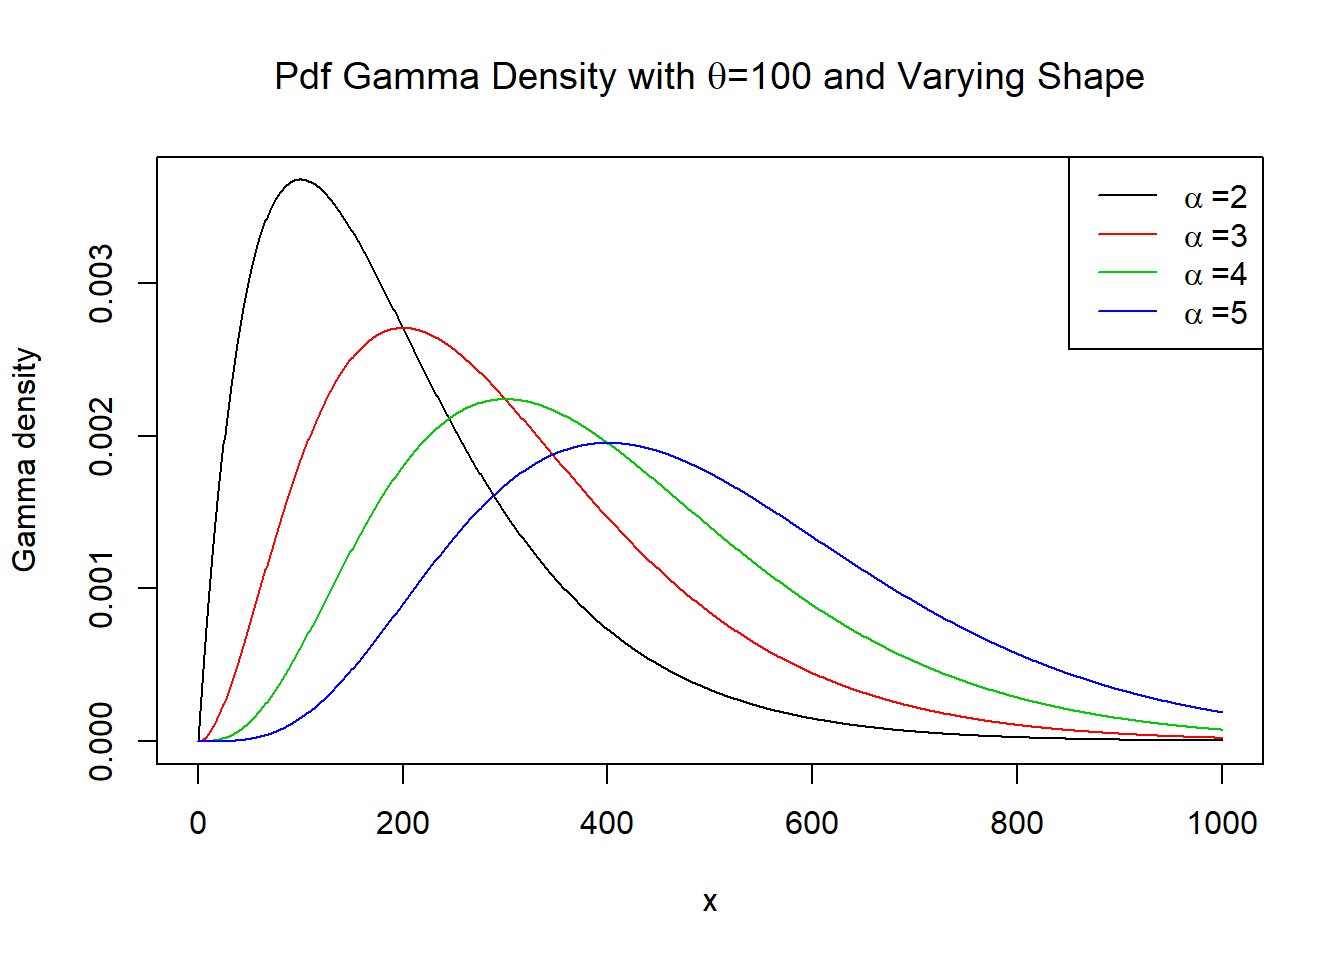
\includegraphics{R_for_Loss_Data_Analytics_files/figure-latex/unnamed-chunk-35-1} \end{center}

A few quick notes on these commands :

\begin{itemize}
\tightlist
\item
  \texttt{seq} is short-hand for sequence
\item
  \texttt{dgamma} function is used for density of the Gamma distribution
  with shape and scale parameters .
\item
  \texttt{plot} is a very handy command for displaying results
  graphically.
\item
  The \texttt{lines()} function is used to add plots to an already
  existing graph.
\item
  The \texttt{legend} function can be used to add legends to plots.
\end{itemize}

\subsection{Varying The Scale
Parameter}\label{varying-the-scale-parameter}

The graph shows the gamma density functions with varying scale
parameters \((\theta)\)

\begin{Shaded}
\begin{Highlighting}[]
\KeywordTok{plot}\NormalTok{(x, }\KeywordTok{dgamma}\NormalTok{(x, }\DataTypeTok{shape =} \DecValTok{2}\NormalTok{, }\DataTypeTok{scale =}\NormalTok{ scale_param[}\DecValTok{1}\NormalTok{]), }\DataTypeTok{type =} \StringTok{"l"}\NormalTok{, }\DataTypeTok{ylab =} \StringTok{"Gamma Density"}\NormalTok{)}

\ControlFlowTok{for}\NormalTok{ (k }\ControlFlowTok{in} \DecValTok{2}\OperatorTok{:}\KeywordTok{length}\NormalTok{(scale_param)) \{}
  \KeywordTok{lines}\NormalTok{(x, }\KeywordTok{dgamma}\NormalTok{(x, }\DataTypeTok{shape =} \DecValTok{2}\NormalTok{, }\DataTypeTok{scale =}\NormalTok{ scale_param[k]), }\DataTypeTok{col =}\NormalTok{ k)}
\NormalTok{\}}

\KeywordTok{legend}\NormalTok{(}\StringTok{"topright"}\NormalTok{, }\KeywordTok{c}\NormalTok{(}\KeywordTok{expression}\NormalTok{(theta }\OperatorTok{~}\StringTok{ '= 100'}\NormalTok{), }\KeywordTok{expression}\NormalTok{(theta }\OperatorTok{~}\StringTok{ '= 150'}\NormalTok{), }
                     \KeywordTok{expression}\NormalTok{(theta }\OperatorTok{~}\StringTok{'= 200'}\NormalTok{), }\KeywordTok{expression}\NormalTok{(theta }\OperatorTok{~}\StringTok{ '= 250'}\NormalTok{)), }
       \DataTypeTok{lty =} \DecValTok{1}\NormalTok{, }\DataTypeTok{col =} \DecValTok{1}\OperatorTok{:}\DecValTok{4}\NormalTok{)}
\KeywordTok{title}\NormalTok{(}\KeywordTok{substitute}\NormalTok{(}\KeywordTok{paste}\NormalTok{(}\StringTok{"Pdf Gamma Density with"}\NormalTok{,}\StringTok{" "}\NormalTok{, alpha, }\StringTok{" = 2"}\NormalTok{, }\StringTok{" "}\NormalTok{, }
                       \StringTok{"and Varying Scale"}\NormalTok{)))}
\end{Highlighting}
\end{Shaded}

\begin{center}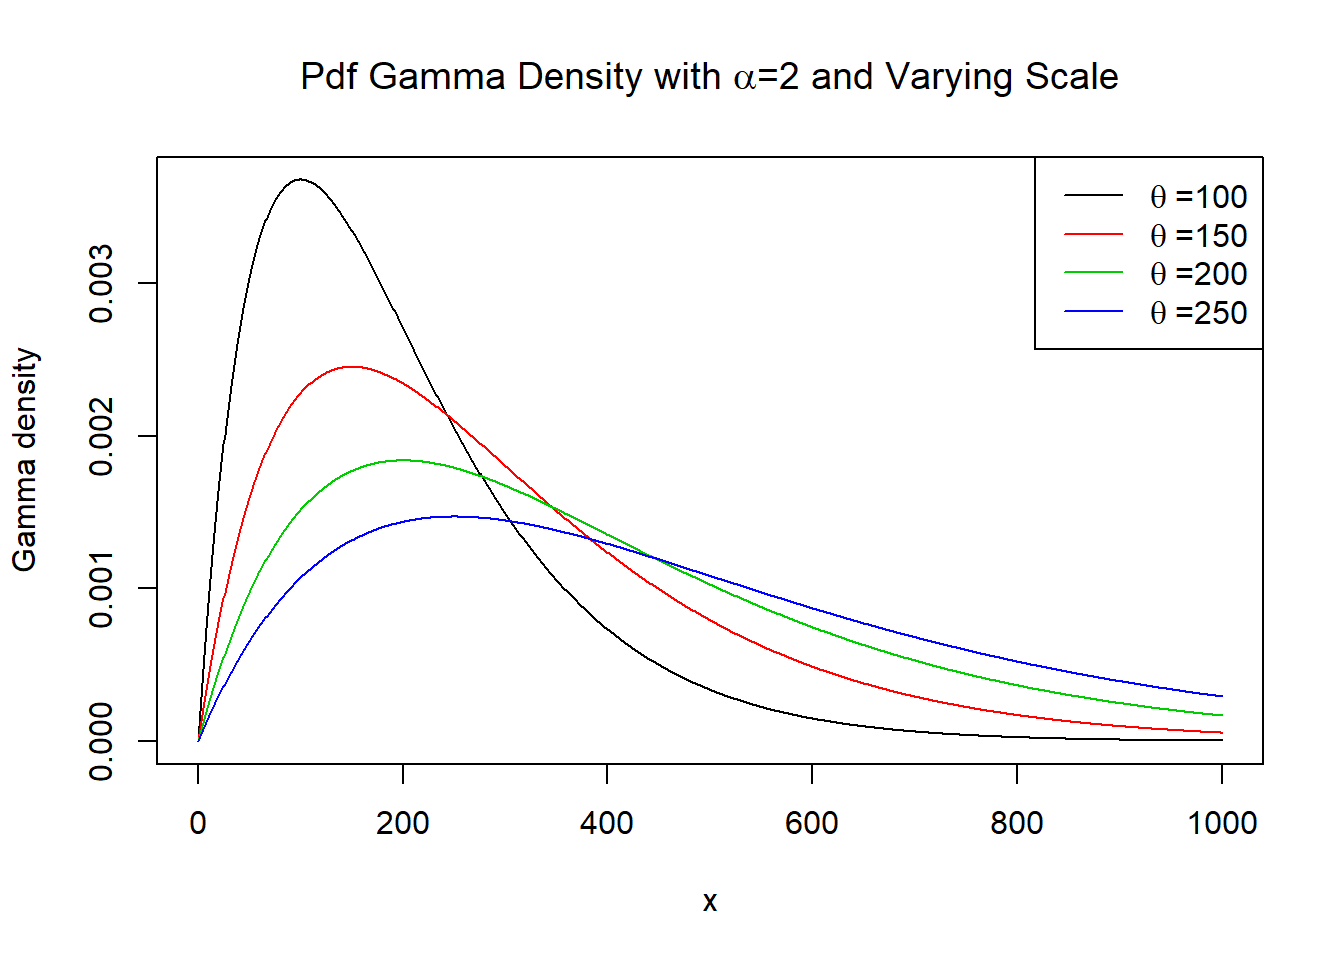
\includegraphics{R_for_Loss_Data_Analytics_files/figure-latex/unnamed-chunk-36-1} \end{center}

\section{Pareto Distribution}\label{pareto-distribution}

This section demonstrates the effect of the shape and scale parameters
on the Pareto density function.

\subsection{Varying The Shape
Parameter}\label{varying-the-shape-parameter-1}

The graph shows the Pareto density functions with varying shape
parameters \((\alpha)\)

\begin{Shaded}
\begin{Highlighting}[]
\NormalTok{z <-}\StringTok{ }\KeywordTok{seq}\NormalTok{(}\DecValTok{0}\NormalTok{, }\DecValTok{3000}\NormalTok{, }\DataTypeTok{by =} \DecValTok{1}\NormalTok{)}

\NormalTok{scale_param <-}\StringTok{ }\KeywordTok{seq}\NormalTok{(}\DecValTok{2000}\NormalTok{, }\DecValTok{3500}\NormalTok{, }\DecValTok{500}\NormalTok{)}
\NormalTok{shape_param <-}\StringTok{ }\DecValTok{1}\OperatorTok{:}\DecValTok{4}

\CommentTok{# Varying the shape parameter}
\KeywordTok{plot}\NormalTok{(z, }\KeywordTok{dparetoII}\NormalTok{(z, }\DataTypeTok{loc =} \DecValTok{0}\NormalTok{, }\DataTypeTok{shape =}\NormalTok{ shape_param[}\DecValTok{1}\NormalTok{], }\DataTypeTok{scale =} \DecValTok{2000}\NormalTok{), }
     \DataTypeTok{ylim =} \KeywordTok{c}\NormalTok{(}\DecValTok{0}\NormalTok{, }\FloatTok{0.002}\NormalTok{),}\DataTypeTok{type =} \StringTok{"l"}\NormalTok{, }\DataTypeTok{ylab =} \StringTok{"Pareto Density"}\NormalTok{)}

\ControlFlowTok{for}\NormalTok{ (k }\ControlFlowTok{in} \DecValTok{2}\OperatorTok{:}\KeywordTok{length}\NormalTok{(shape_param)) \{}
  \KeywordTok{lines}\NormalTok{(z, }\KeywordTok{dparetoII}\NormalTok{(z,}\DataTypeTok{loc =} \DecValTok{0}\NormalTok{, }\DataTypeTok{shape =}\NormalTok{ shape_param[k], }\DataTypeTok{scale =} \DecValTok{2000}\NormalTok{), }\DataTypeTok{col =}\NormalTok{ k)}
\NormalTok{\}}
\KeywordTok{legend}\NormalTok{(}\StringTok{"topright"}\NormalTok{, }\KeywordTok{c}\NormalTok{(}\KeywordTok{expression}\NormalTok{(alpha }\OperatorTok{~}\StringTok{ '= 1'}\NormalTok{), }\KeywordTok{expression}\NormalTok{(alpha }\OperatorTok{~}\StringTok{ '= 2'}\NormalTok{), }
                     \KeywordTok{expression}\NormalTok{(alpha }\OperatorTok{~}\StringTok{ '= 3'}\NormalTok{), }\KeywordTok{expression}\NormalTok{(alpha }\OperatorTok{~}\StringTok{ '= 4'}\NormalTok{)), }
       \DataTypeTok{lty =} \DecValTok{1}\NormalTok{, }\DataTypeTok{col =} \DecValTok{1}\OperatorTok{:}\DecValTok{4}\NormalTok{)}
\KeywordTok{title}\NormalTok{(}\KeywordTok{substitute}\NormalTok{(}\KeywordTok{paste}\NormalTok{(}\StringTok{"Pdf Pareto Density with"}\NormalTok{,}\StringTok{" "}\NormalTok{,theta,}\StringTok{" = 2000"}\NormalTok{,}\StringTok{" "}\NormalTok{, }
                       \StringTok{"and Varying Shape"}\NormalTok{)))}
\end{Highlighting}
\end{Shaded}

\begin{center}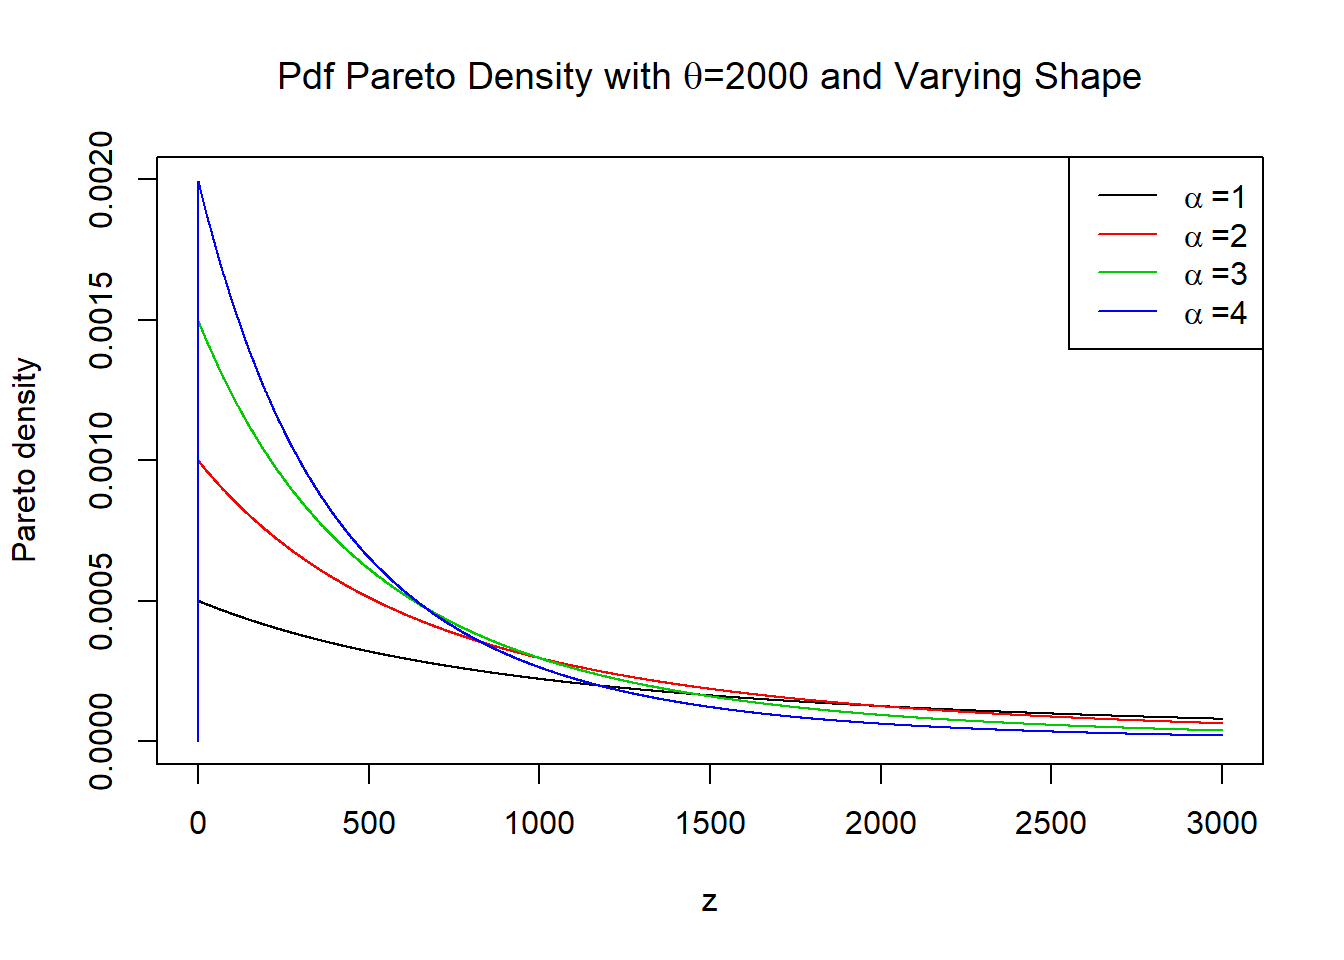
\includegraphics{R_for_Loss_Data_Analytics_files/figure-latex/unnamed-chunk-38-1} \end{center}

\subsection{Varying The Scale
Parameter}\label{varying-the-scale-parameter-1}

The graph shows the Pareto density functions with varying scale
parameters \((\theta)\)

\begin{Shaded}
\begin{Highlighting}[]
\KeywordTok{plot}\NormalTok{(z, }\KeywordTok{dparetoII}\NormalTok{(z, }\DataTypeTok{loc =} \DecValTok{0}\NormalTok{, }\DataTypeTok{shape =} \DecValTok{3}\NormalTok{, }\DataTypeTok{scale =}\NormalTok{ scale_param[}\DecValTok{1}\NormalTok{]), }
     \DataTypeTok{type =} \StringTok{"l"}\NormalTok{, }\DataTypeTok{ylab =} \StringTok{"Pareto Density"}\NormalTok{)}

\ControlFlowTok{for}\NormalTok{ (k }\ControlFlowTok{in} \DecValTok{2}\OperatorTok{:}\KeywordTok{length}\NormalTok{(scale_param)) \{}
  \KeywordTok{lines}\NormalTok{(z, }\KeywordTok{dparetoII}\NormalTok{(z, }\DataTypeTok{loc =} \DecValTok{0}\NormalTok{, }\DataTypeTok{shape =} \DecValTok{3}\NormalTok{, }\DataTypeTok{scale =}\NormalTok{ scale_param[k]), }\DataTypeTok{col =}\NormalTok{ k)}
\NormalTok{\}}

\KeywordTok{legend}\NormalTok{(}\StringTok{"topright"}\NormalTok{, }\KeywordTok{c}\NormalTok{(}\KeywordTok{expression}\NormalTok{(theta }\OperatorTok{~}\StringTok{ '= 2000'}\NormalTok{), }\KeywordTok{expression}\NormalTok{(theta }\OperatorTok{~}\StringTok{ '= 2500'}\NormalTok{), }
                     \KeywordTok{expression}\NormalTok{(theta }\OperatorTok{~}\StringTok{ '= 3000'}\NormalTok{), }\KeywordTok{expression}\NormalTok{(theta }\OperatorTok{~}\StringTok{ '= 3500'}\NormalTok{)), }
       \DataTypeTok{lty =} \DecValTok{1}\NormalTok{, }\DataTypeTok{col =} \DecValTok{1}\OperatorTok{:}\DecValTok{4}\NormalTok{)}
\KeywordTok{title}\NormalTok{(}\KeywordTok{substitute}\NormalTok{(}\KeywordTok{paste}\NormalTok{(}\StringTok{"Pdf Pareto Density with"}\NormalTok{,}\StringTok{" "}\NormalTok{,alpha,}\StringTok{" = 3"}\NormalTok{,}\StringTok{" "}\NormalTok{, }
                       \StringTok{"and Varying Scale"}\NormalTok{)))}
\end{Highlighting}
\end{Shaded}

\begin{center}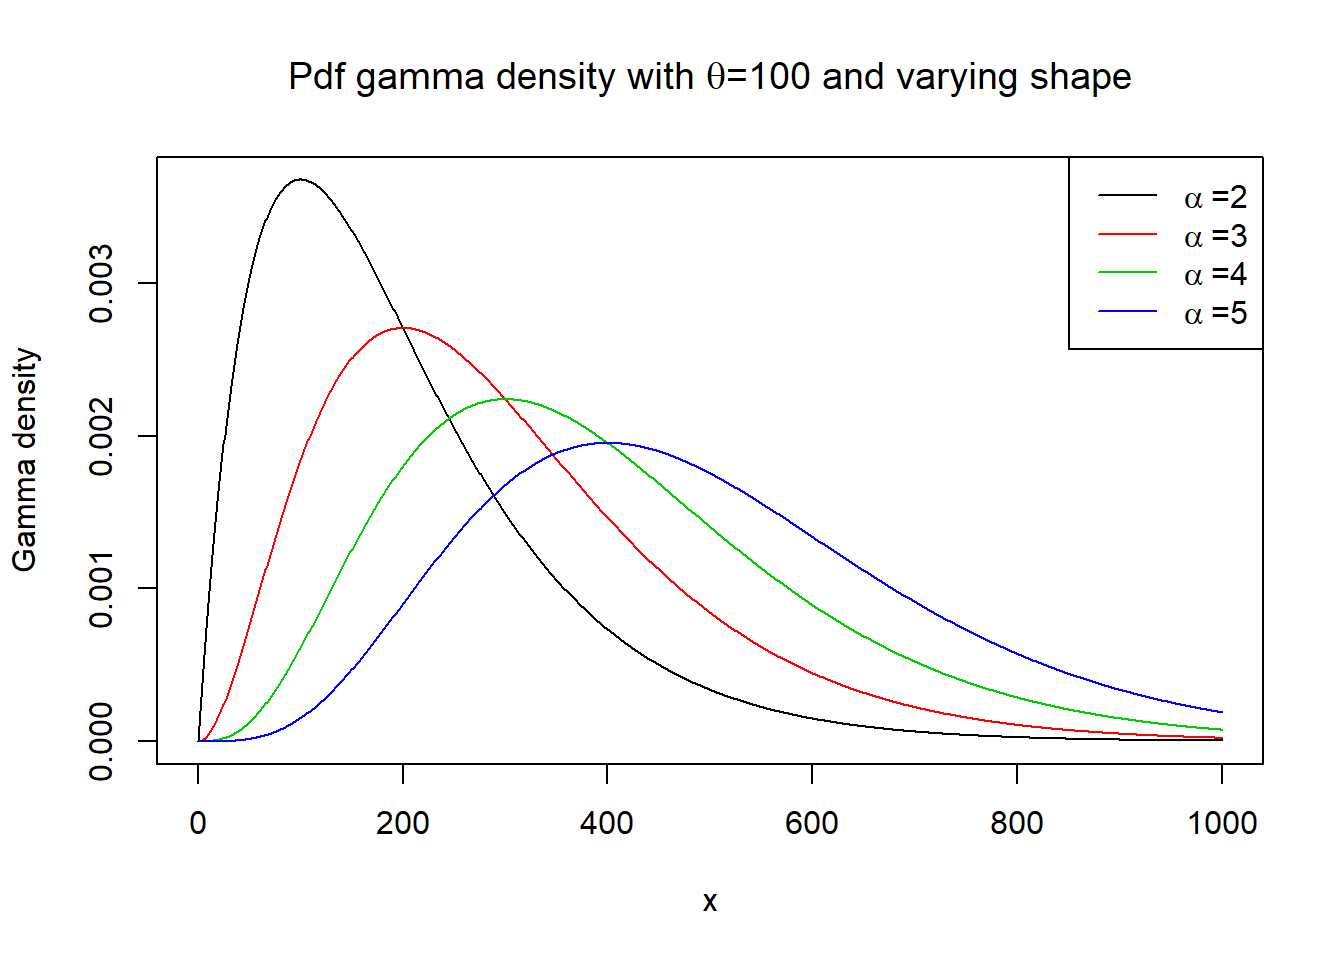
\includegraphics{R_for_Loss_Data_Analytics_files/figure-latex/unnamed-chunk-39-1} \end{center}

\section{Weibull Distribution}\label{weibull-distribution}

This section demonstrates the effect of the shape and scale parameters
on the Weibull density function.

\subsection{Varying The Shape
Parameter}\label{varying-the-shape-parameter-2}

The graph shows the Weibull density function with varying shape
parameters \((\alpha)\)

\begin{Shaded}
\begin{Highlighting}[]
\NormalTok{z <-}\StringTok{ }\KeywordTok{seq}\NormalTok{(}\DecValTok{0}\NormalTok{, }\DecValTok{400}\NormalTok{, }\DataTypeTok{by =} \DecValTok{1}\NormalTok{)}

\NormalTok{scale_param <-}\StringTok{ }\KeywordTok{seq}\NormalTok{(}\DecValTok{50}\NormalTok{, }\DecValTok{200}\NormalTok{, }\DecValTok{50}\NormalTok{)}
\NormalTok{shape_param <-}\StringTok{ }\KeywordTok{seq}\NormalTok{(}\FloatTok{1.5}\NormalTok{, }\DecValTok{3}\NormalTok{, }\FloatTok{0.5}\NormalTok{)}

\CommentTok{# Varying the shape parameter}
\KeywordTok{plot}\NormalTok{(z, }\KeywordTok{dweibull}\NormalTok{(z, }\DataTypeTok{shape =}\NormalTok{ shape_param[}\DecValTok{1}\NormalTok{], }\DataTypeTok{scale =} \DecValTok{100}\NormalTok{), }
     \DataTypeTok{ylim =} \KeywordTok{c}\NormalTok{(}\DecValTok{0}\NormalTok{, }\FloatTok{0.012}\NormalTok{), }\DataTypeTok{type =} \StringTok{"l"}\NormalTok{, }\DataTypeTok{ylab =} \StringTok{"Weibull Density"}\NormalTok{)}

\ControlFlowTok{for}\NormalTok{ (k }\ControlFlowTok{in} \DecValTok{2}\OperatorTok{:}\KeywordTok{length}\NormalTok{(shape_param)) \{}
  \KeywordTok{lines}\NormalTok{(z, }\KeywordTok{dweibull}\NormalTok{(z, }\DataTypeTok{shape =}\NormalTok{ shape_param[k], }\DataTypeTok{scale =} \DecValTok{100}\NormalTok{), }\DataTypeTok{col =}\NormalTok{ k)}
\NormalTok{\}}

\KeywordTok{legend}\NormalTok{(}\StringTok{"topright"}\NormalTok{,  }\KeywordTok{c}\NormalTok{(}\KeywordTok{expression}\NormalTok{(alpha }\OperatorTok{~}\StringTok{ '= 1.5'}\NormalTok{), }\KeywordTok{expression}\NormalTok{(alpha }\OperatorTok{~}\StringTok{ '= 2'}\NormalTok{), }
                      \KeywordTok{expression}\NormalTok{(alpha }\OperatorTok{~}\StringTok{'= 2.5'}\NormalTok{), }\KeywordTok{expression}\NormalTok{(alpha }\OperatorTok{~}\StringTok{ '= 3'}\NormalTok{)), }
       \DataTypeTok{lty =} \DecValTok{1}\NormalTok{, }\DataTypeTok{col =} \DecValTok{1}\OperatorTok{:}\DecValTok{4}\NormalTok{)}
\KeywordTok{title}\NormalTok{(}\KeywordTok{substitute}\NormalTok{(}\KeywordTok{paste}\NormalTok{(}\StringTok{"Pdf Weibull Density with"}\NormalTok{,}\StringTok{" "}\NormalTok{,theta,}\StringTok{" = 100"}\NormalTok{,}\StringTok{" "}\NormalTok{, }
                       \StringTok{"and Varying Shape"}\NormalTok{)))}
\end{Highlighting}
\end{Shaded}

\begin{center}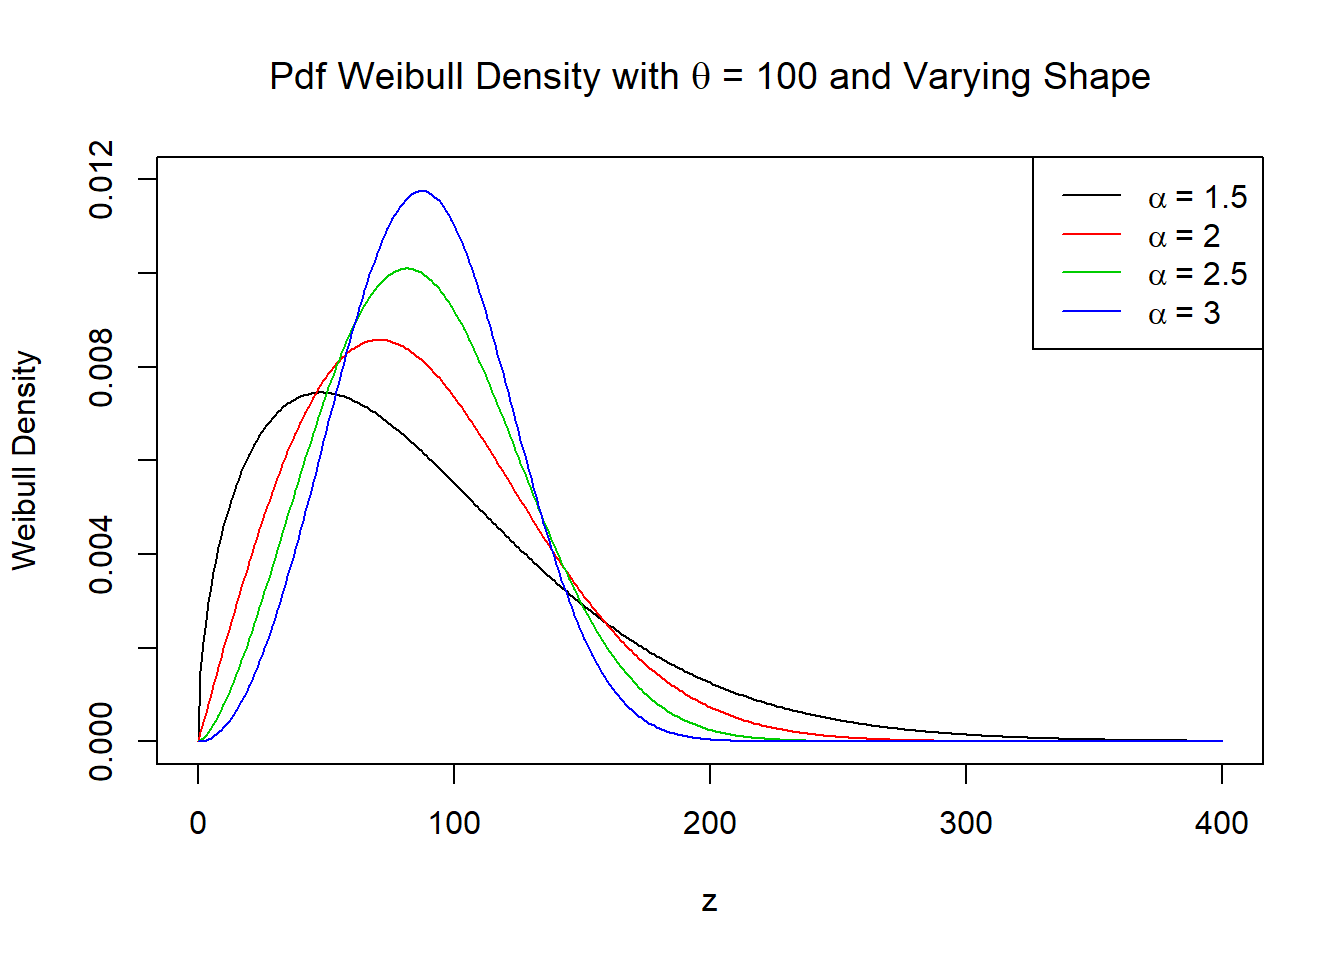
\includegraphics{R_for_Loss_Data_Analytics_files/figure-latex/unnamed-chunk-40-1} \end{center}

\subsection{Varying The Scale
Parameter}\label{varying-the-scale-parameter-2}

The graph shows the Weibull density function with varying scale
parameters \((\theta)\)

\begin{Shaded}
\begin{Highlighting}[]
\KeywordTok{plot}\NormalTok{(z, }\KeywordTok{dweibull}\NormalTok{(z, }\DataTypeTok{shape =} \DecValTok{3}\NormalTok{, }\DataTypeTok{scale =}\NormalTok{ scale_param[}\DecValTok{1}\NormalTok{]), }
     \DataTypeTok{type =} \StringTok{"l"}\NormalTok{, }\DataTypeTok{ylab =} \StringTok{"Weibull Density"}\NormalTok{)}

\ControlFlowTok{for}\NormalTok{(k }\ControlFlowTok{in} \DecValTok{2}\OperatorTok{:}\KeywordTok{length}\NormalTok{(scale_param))\{}
  \KeywordTok{lines}\NormalTok{(z,}\KeywordTok{dweibull}\NormalTok{(z, }\DataTypeTok{shape =} \DecValTok{3}\NormalTok{, }\DataTypeTok{scale =}\NormalTok{ scale_param[k]), }\DataTypeTok{col =}\NormalTok{ k)}
\NormalTok{\}}
\KeywordTok{legend}\NormalTok{(}\StringTok{"topright"}\NormalTok{, }\KeywordTok{c}\NormalTok{(}\KeywordTok{expression}\NormalTok{(theta }\OperatorTok{~}\StringTok{ '= 50'}\NormalTok{), }\KeywordTok{expression}\NormalTok{(theta }\OperatorTok{~}\StringTok{ '= 100'}\NormalTok{), }
                     \KeywordTok{expression}\NormalTok{(theta }\OperatorTok{~}\StringTok{ '= 150'}\NormalTok{), }\KeywordTok{expression}\NormalTok{(theta }\OperatorTok{~}\StringTok{ '= 200'}\NormalTok{)), }
       \DataTypeTok{lty =} \DecValTok{1}\NormalTok{, }\DataTypeTok{col =} \DecValTok{1}\OperatorTok{:}\DecValTok{4}\NormalTok{)}
\KeywordTok{title}\NormalTok{(}\KeywordTok{substitute}\NormalTok{(}\KeywordTok{paste}\NormalTok{(}\StringTok{"Pdf Weibull Density with"}\NormalTok{, }\StringTok{" "}\NormalTok{, alpha, }\StringTok{" = 3"}\NormalTok{, }\StringTok{" "}\NormalTok{, }
                       \StringTok{"and Varying Scale"}\NormalTok{)))}
\end{Highlighting}
\end{Shaded}

\begin{center}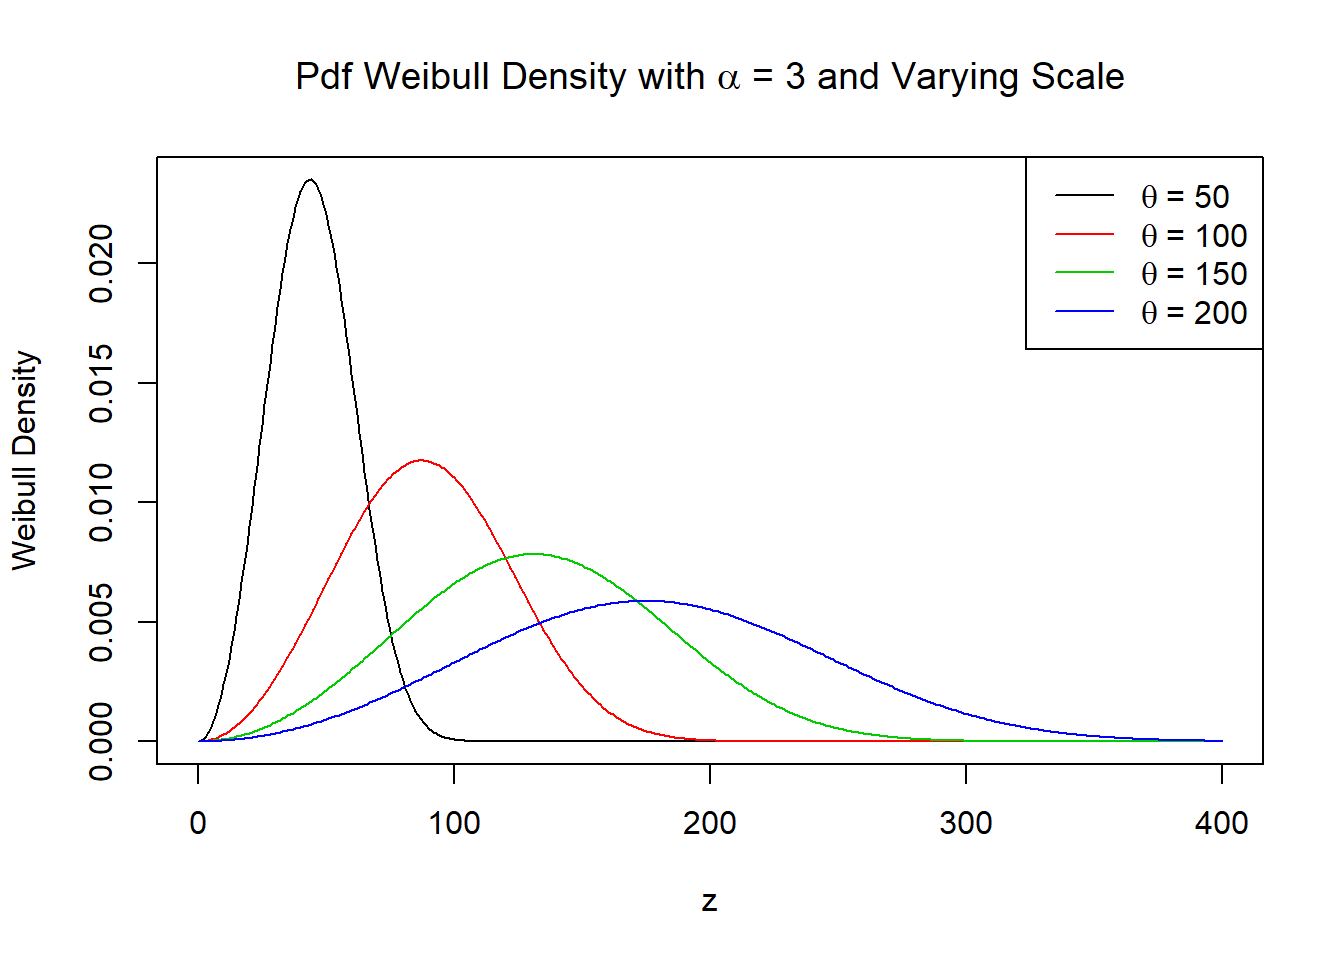
\includegraphics{R_for_Loss_Data_Analytics_files/figure-latex/unnamed-chunk-41-1} \end{center}

\section{Generalized Beta Distribution of The Second Kind
(GB2)}\label{generalized-beta-distribution-of-the-second-kind-gb2}

This section demonstrates the effect of the shape and scale parameters
on the GB2 density function.

\subsection{Varying The Scale
Parameter}\label{varying-the-scale-parameter-3}

The graph shows the GB2 density function with varying scale parameter
\((\theta)\)

\begin{Shaded}
\begin{Highlighting}[]
\CommentTok{# Example 4:GB2}
\NormalTok{gb2_density <-}\StringTok{ }\ControlFlowTok{function}\NormalTok{ (x, shape_}\DecValTok{1}\NormalTok{, shape_}\DecValTok{2}\NormalTok{, shape_}\DecValTok{3}\NormalTok{, scale)\{}
\NormalTok{  mu <-}\StringTok{ }\KeywordTok{log}\NormalTok{(scale)}
\NormalTok{  sigma <-}\StringTok{ }\DecValTok{1} \OperatorTok{/}\StringTok{ }\NormalTok{shape_}\DecValTok{3}
\NormalTok{  xt <-}\StringTok{ }\NormalTok{(}\KeywordTok{log}\NormalTok{(x) }\OperatorTok{-}\StringTok{ }\NormalTok{mu) }\OperatorTok{/}\StringTok{ }\NormalTok{sigma}
\NormalTok{  logexpxt <-}\StringTok{ }\KeywordTok{ifelse}\NormalTok{ (xt }\OperatorTok{>}\StringTok{ }\DecValTok{23}\NormalTok{, yt, }\KeywordTok{log}\NormalTok{(}\DecValTok{1} \OperatorTok{+}\StringTok{ }\KeywordTok{exp}\NormalTok{(xt)))}
\NormalTok{  logdens <-}\StringTok{ }\NormalTok{shape_}\DecValTok{1} \OperatorTok{*}\StringTok{ }\NormalTok{xt }\OperatorTok{-}\StringTok{ }\KeywordTok{log}\NormalTok{(sigma) }\OperatorTok{-}\StringTok{ }\KeywordTok{log}\NormalTok{(}\KeywordTok{beta}\NormalTok{(shape_}\DecValTok{1}\NormalTok{, shape_}\DecValTok{2}\NormalTok{)) }\OperatorTok{-}\StringTok{ }
\StringTok{    }\NormalTok{(shape_}\DecValTok{1} \OperatorTok{+}\StringTok{ }\NormalTok{shape_}\DecValTok{2}\NormalTok{) }\OperatorTok{*}\StringTok{ }\NormalTok{logexpxt }\OperatorTok{-}\StringTok{ }\KeywordTok{log}\NormalTok{(x) }
  \KeywordTok{exp}\NormalTok{(logdens)}
\NormalTok{\}}
\NormalTok{x <-}\StringTok{ }\KeywordTok{seq}\NormalTok{(}\DecValTok{0}\NormalTok{, }\DecValTok{400}\NormalTok{, }\DataTypeTok{by =} \DecValTok{1}\NormalTok{)}

\NormalTok{alpha_}\DecValTok{1}\NormalTok{ <-}\StringTok{ }\DecValTok{5}
\NormalTok{alpha_}\DecValTok{2}\NormalTok{ <-}\StringTok{ }\DecValTok{4} 
\NormalTok{gamma <-}\StringTok{ }\DecValTok{2}
\NormalTok{theta <-}\StringTok{ }\KeywordTok{seq}\NormalTok{(}\DecValTok{150}\NormalTok{, }\DecValTok{250}\NormalTok{, }\DecValTok{50}\NormalTok{)}

\CommentTok{# Varying the scale parameter}
\KeywordTok{plot}\NormalTok{(x, }
     \KeywordTok{gb2_density}\NormalTok{(x, }\DataTypeTok{shape_1 =}\NormalTok{ alpha_}\DecValTok{1}\NormalTok{, }\DataTypeTok{shape_2 =}\NormalTok{ alpha_}\DecValTok{2}\NormalTok{, }\DataTypeTok{shape_3 =}\NormalTok{ gamma, }
                 \DataTypeTok{scale =}\NormalTok{ theta[}\DecValTok{1}\NormalTok{]), }\DataTypeTok{type =} \StringTok{"l"}\NormalTok{, }\DataTypeTok{ylab =} \StringTok{"Gen Beta 2 Density"}\NormalTok{, }
     \DataTypeTok{main =} \KeywordTok{expression}\NormalTok{(}\KeywordTok{paste}\NormalTok{(}\StringTok{"GB2 Density with "}\NormalTok{, alpha[}\DecValTok{1}\NormalTok{], }\StringTok{" = 5, "}\NormalTok{, }
\NormalTok{                             alpha[}\DecValTok{2}\NormalTok{], }\StringTok{" = 4, "}\NormalTok{, alpha[}\DecValTok{3}\NormalTok{], }\StringTok{" = 2, "}\NormalTok{, }
                             \StringTok{"and Varying Scale ("}\NormalTok{, theta, }\StringTok{") Parameters"}\NormalTok{)), }
     \DataTypeTok{cex.main =} \FloatTok{0.95}\NormalTok{ )}

\ControlFlowTok{for}\NormalTok{(k }\ControlFlowTok{in} \DecValTok{2}\OperatorTok{:}\KeywordTok{length}\NormalTok{(theta))\{}
  \KeywordTok{lines}\NormalTok{(x, }\KeywordTok{gb2_density}\NormalTok{(x, }\DataTypeTok{shape_1 =}\NormalTok{ alpha_}\DecValTok{1}\NormalTok{, }\DataTypeTok{shape_2 =}\NormalTok{ alpha_}\DecValTok{2}\NormalTok{, }\DataTypeTok{shape_3 =}\NormalTok{ gamma, }
                       \DataTypeTok{scale =}\NormalTok{ theta[k]), }\DataTypeTok{col =}\NormalTok{ k)}
\NormalTok{\}}
\KeywordTok{legend}\NormalTok{(}\StringTok{"topleft"}\NormalTok{, }\KeywordTok{c}\NormalTok{(}\KeywordTok{expression}\NormalTok{(theta }\OperatorTok{~}\StringTok{ '= 150'}\NormalTok{), }\KeywordTok{expression}\NormalTok{(theta }\OperatorTok{~}\StringTok{ '= 200'}\NormalTok{), }
                    \KeywordTok{expression}\NormalTok{(theta }\OperatorTok{~}\StringTok{ '= 250'}\NormalTok{)), }\DataTypeTok{lty =} \DecValTok{1}\NormalTok{, }\DataTypeTok{cex =} \FloatTok{0.6}\NormalTok{, }\DataTypeTok{col =} \DecValTok{1}\OperatorTok{:}\DecValTok{3}\NormalTok{)}
\end{Highlighting}
\end{Shaded}

\begin{center}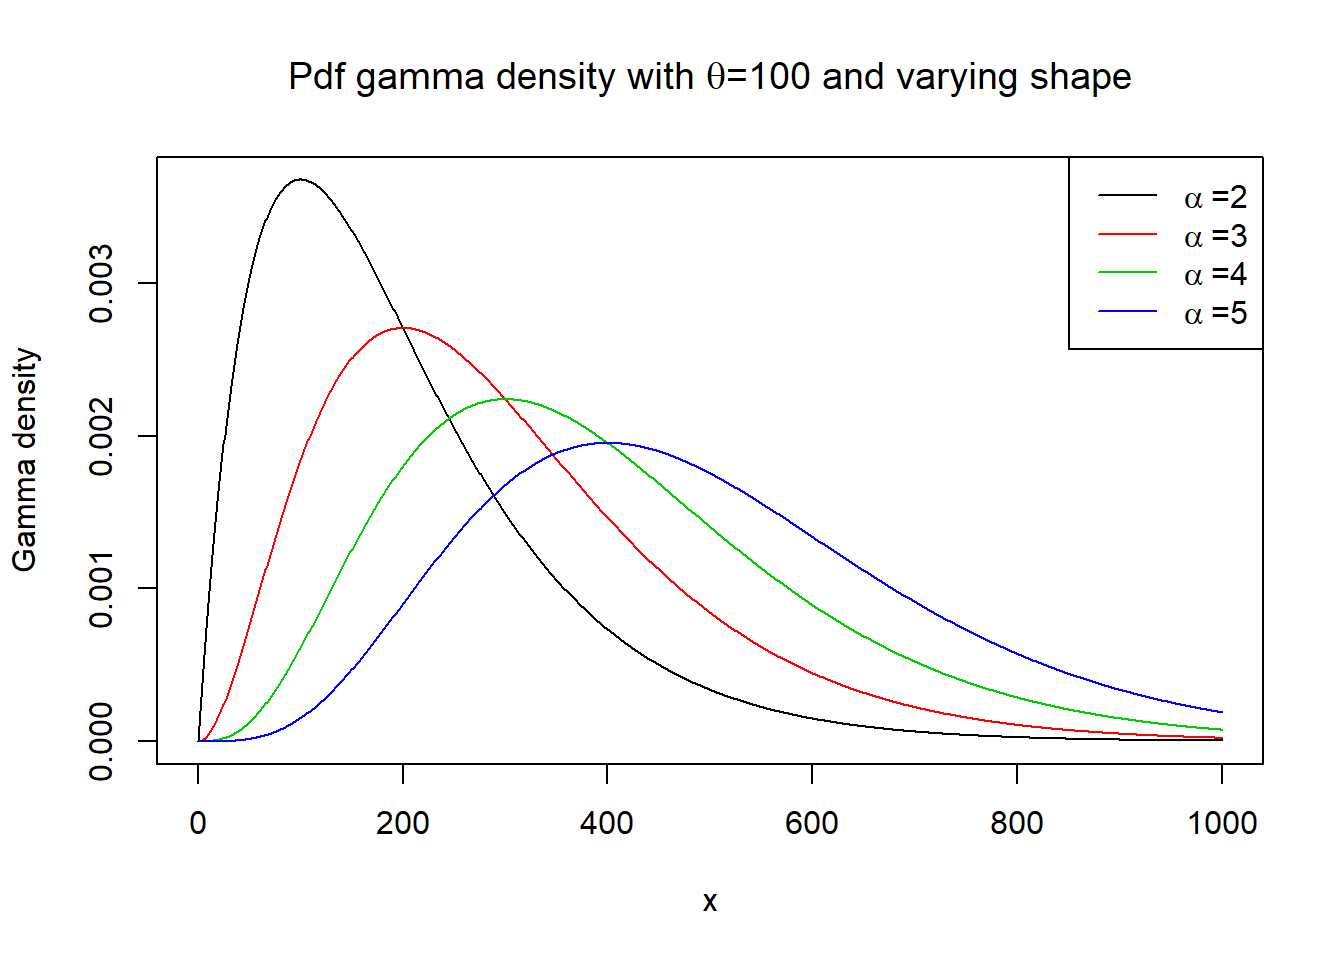
\includegraphics{R_for_Loss_Data_Analytics_files/figure-latex/unnamed-chunk-42-1} \end{center}

Note: Here we wrote our own function for the density function of the GB2
density function.

\section{Methods of Creating New
Distributions}\label{methods-of-creating-new-distributions}

This section shows some of the methods of creating new distributions.

\subsection{Mixture Distributions}\label{mixture-distributions}

The graph below creates a density function from two random variables
that follow a gamma distribution.

\begin{Shaded}
\begin{Highlighting}[]
\CommentTok{# Example 5: A mixed density}
\CommentTok{# Specify density of a mixture of 2 gamma distributions}
\NormalTok{mixture_gamma_density <-}\StringTok{ }\ControlFlowTok{function}\NormalTok{ (x, a_}\DecValTok{1}\NormalTok{, a_}\DecValTok{2}\NormalTok{, alpha_gamma1, theta_gamma1, alpha_gamma2,}
\NormalTok{                                   theta_gamma2)\{}
\NormalTok{  a_}\DecValTok{1} \OperatorTok{*}\StringTok{ }\KeywordTok{dgamma}\NormalTok{(x, }\DataTypeTok{shape =}\NormalTok{ alpha_gamma1, }\DataTypeTok{scale =}\NormalTok{ theta_gamma1) }\OperatorTok{+}\StringTok{ }\NormalTok{a_}\DecValTok{2} \OperatorTok{*}\StringTok{ }
\StringTok{    }\KeywordTok{dgamma}\NormalTok{(x, }\DataTypeTok{shape =}\NormalTok{ alpha_gamma2, }\DataTypeTok{scale =}\NormalTok{ theta_gamma2)}
\NormalTok{\}}

\NormalTok{w <-}\StringTok{ }\DecValTok{1}\OperatorTok{:}\DecValTok{30000} \OperatorTok{/}\StringTok{ }\DecValTok{100}
\NormalTok{a_}\DecValTok{1}\NormalTok{ <-}\StringTok{ }\FloatTok{0.5}
\NormalTok{a_}\DecValTok{2}\NormalTok{ <-}\StringTok{ }\FloatTok{0.5}
\NormalTok{alpha_}\DecValTok{1}\NormalTok{ <-}\StringTok{ }\DecValTok{4}
\NormalTok{theta_}\DecValTok{1}\NormalTok{ <-}\StringTok{ }\DecValTok{7}
\NormalTok{alpha_}\DecValTok{2}\NormalTok{ <-}\StringTok{ }\DecValTok{15}
\NormalTok{theta_}\DecValTok{2}\NormalTok{ <-}\StringTok{ }\DecValTok{7}

\NormalTok{mix_gamma_dens <-}\StringTok{ }\KeywordTok{mixture_gamma_density}\NormalTok{(w, a_}\DecValTok{1}\NormalTok{, a_}\DecValTok{2}\NormalTok{, alpha_}\DecValTok{1}\NormalTok{, theta_}\DecValTok{1}\NormalTok{, alpha_}\DecValTok{2}\NormalTok{, theta_}\DecValTok{2}\NormalTok{)}

\KeywordTok{plot}\NormalTok{(w, mix_gamma_dens, }\DataTypeTok{type =} \StringTok{"l"}\NormalTok{)}
\end{Highlighting}
\end{Shaded}

\begin{center}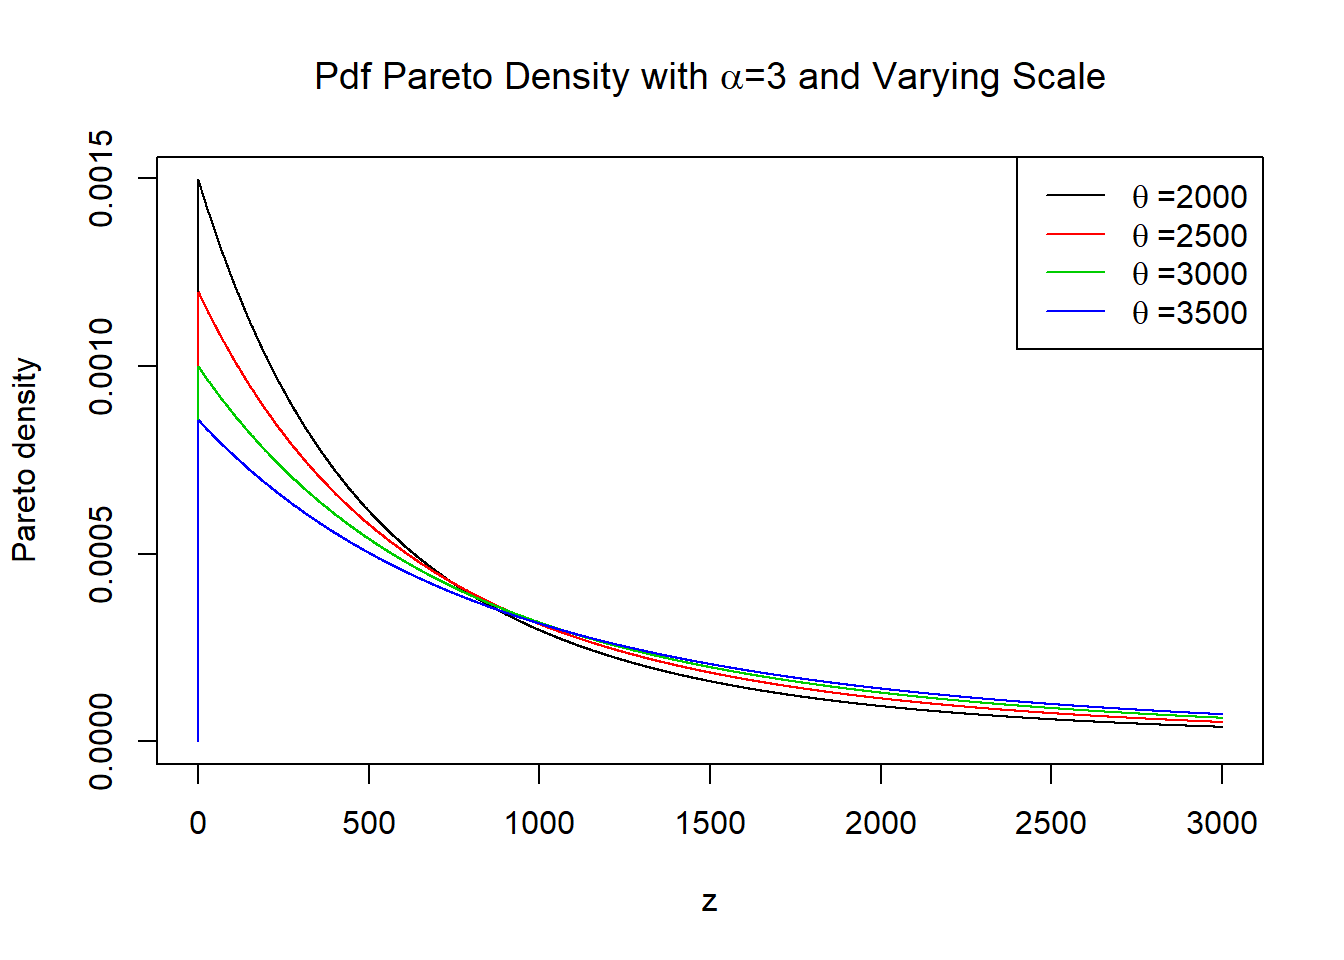
\includegraphics{R_for_Loss_Data_Analytics_files/figure-latex/unnamed-chunk-43-1} \end{center}

\subsection{Density Obtained Through
Splicing}\label{density-obtained-through-splicing}

The graph below shows a density function through splicing by combining
an exponential distribution on \((0,c)\) with a Pareto distribution on
\((c,\infty)\)

\begin{Shaded}
\begin{Highlighting}[]
\CommentTok{# Example 6: density obtained through splicing}
\CommentTok{# Combine an Exp on (0,c) with a Pareto on (c,\textbackslash{}infty)}

\NormalTok{splice_exp_par <-}\StringTok{ }\ControlFlowTok{function}\NormalTok{ (x, c, v, theta, gamma, alpha)\{}
  \ControlFlowTok{if}\NormalTok{ (}\DecValTok{0} \OperatorTok{<=}\StringTok{ }\NormalTok{x }\OperatorTok{&}\StringTok{ }\NormalTok{x }\OperatorTok{<}\StringTok{ }\NormalTok{c) \{}\KeywordTok{return}\NormalTok{(v }\OperatorTok{*}\StringTok{ }\KeywordTok{dexp}\NormalTok{(x, }\DecValTok{1} \OperatorTok{/}\StringTok{ }\NormalTok{theta) }\OperatorTok{/}\StringTok{ }\KeywordTok{pexp}\NormalTok{(c, }\DecValTok{1} \OperatorTok{/}\StringTok{ }\NormalTok{theta))\} }\ControlFlowTok{else} 
    \ControlFlowTok{if}\NormalTok{ (x }\OperatorTok{>=}\StringTok{ }\NormalTok{c) \{}\KeywordTok{return}\NormalTok{((}\DecValTok{1} \OperatorTok{-}\StringTok{ }\NormalTok{v) }\OperatorTok{*}\StringTok{ }\KeywordTok{dparetoII}\NormalTok{(x, }\DataTypeTok{loc =} \DecValTok{0}\NormalTok{, }\DataTypeTok{shape =}\NormalTok{ alpha, }\DataTypeTok{scale =}\NormalTok{ theta) }\OperatorTok{/}\StringTok{ }
\StringTok{                          }\NormalTok{(}\DecValTok{1} \OperatorTok{-}\StringTok{ }\KeywordTok{pparetoII}\NormalTok{(x, }\DataTypeTok{loc =} \DecValTok{0}\NormalTok{, }\DataTypeTok{shape =}\NormalTok{ alpha, }\DataTypeTok{scale =}\NormalTok{ theta)))\}}
\NormalTok{\}}

\NormalTok{x <-}\StringTok{ }\KeywordTok{t}\NormalTok{(}\KeywordTok{as.matrix}\NormalTok{(}\DecValTok{1}\OperatorTok{:}\DecValTok{2500} \OperatorTok{/}\StringTok{ }\DecValTok{10}\NormalTok{))}

\NormalTok{splice_values <-}\StringTok{ }\KeywordTok{apply}\NormalTok{(x, }\DecValTok{2}\NormalTok{, splice_exp_par, }\DataTypeTok{c =} \DecValTok{100}\NormalTok{, }\DataTypeTok{v =} \FloatTok{0.6}\NormalTok{, }
                       \DataTypeTok{theta =} \DecValTok{100}\NormalTok{, }\DataTypeTok{gamma =} \DecValTok{200}\NormalTok{, }\DataTypeTok{alpha =} \DecValTok{4}\NormalTok{)}

\KeywordTok{plot}\NormalTok{(x, splice_values, }\DataTypeTok{type =} \StringTok{'l'}\NormalTok{)}
\end{Highlighting}
\end{Shaded}

\begin{center}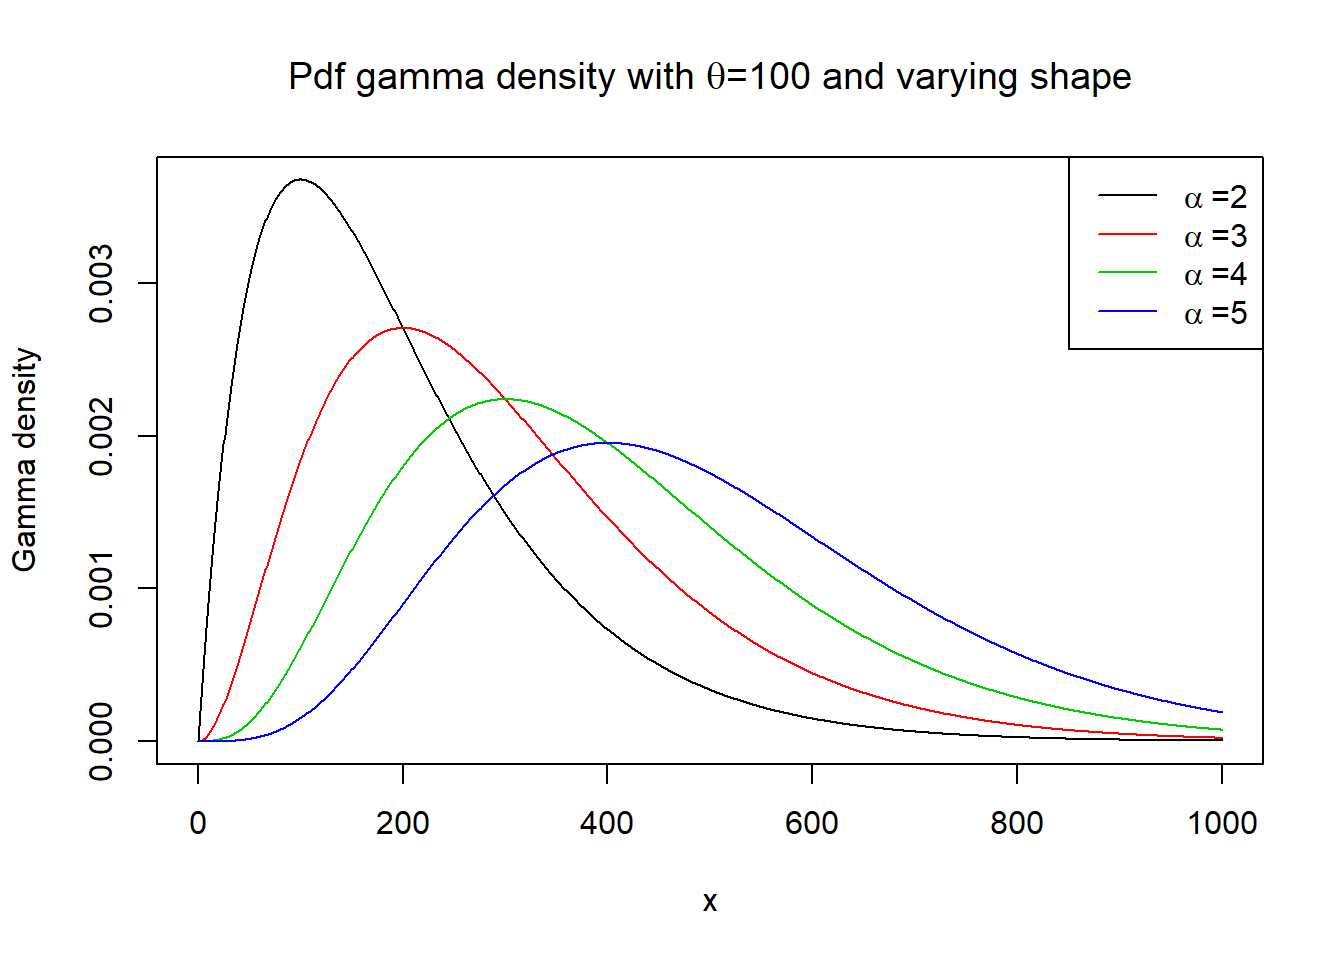
\includegraphics{R_for_Loss_Data_Analytics_files/figure-latex/unnamed-chunk-44-1} \end{center}

\section{Coverage Modifications}\label{coverage-modifications}

\subsection{Load Required Package}\label{load-required-package}

The \texttt{actuar} package provides functions for dealing with coverage
modifications. In the following sections we will check the
functionalities of the \texttt{coverage} command.

\begin{Shaded}
\begin{Highlighting}[]
\KeywordTok{library}\NormalTok{(actuar)}
\end{Highlighting}
\end{Shaded}

\subsection{Ordinary Deductible}\label{ordinary-deductible}

This section plots the modified probability density functions due to
deductibles for the payment per loss and payment per payment random
variables.

\subsubsection{Payment Per Loss with Ordinary
Deductible}\label{payment-per-loss-with-ordinary-deductible}

Let \(X\) be the random variable for loss size. The random variable for
the payment per loss with deductible \(d\) is \(Y^L=(X-d)_+\). The plot
of the modified probability density function is below.

\begin{Shaded}
\begin{Highlighting}[]
\NormalTok{f <-}\StringTok{ }\KeywordTok{coverage}\NormalTok{(dgamma, pgamma, }\DataTypeTok{deductible =} \DecValTok{1}\NormalTok{, }\DataTypeTok{per.loss =} \OtherTok{TRUE}\NormalTok{)  }\CommentTok{# create the object}
\KeywordTok{mode}\NormalTok{(f)  }\CommentTok{# it's a function. Here deductible is 1}
\end{Highlighting}
\end{Shaded}

\begin{verbatim}
[1] "function"
\end{verbatim}

\begin{Shaded}
\begin{Highlighting}[]
\CommentTok{# Check the pdf for Y^L at 0 and the original loss at 1}
\KeywordTok{f}\NormalTok{(}\DecValTok{0}\NormalTok{, }\DecValTok{3}\NormalTok{)  }\CommentTok{# mass at 0}
\end{Highlighting}
\end{Shaded}

\begin{verbatim}
[1] 0.0803014
\end{verbatim}

\begin{Shaded}
\begin{Highlighting}[]
\KeywordTok{pgamma}\NormalTok{(}\DecValTok{0} \OperatorTok{+}\StringTok{ }\DecValTok{1}\NormalTok{, }\DecValTok{3}\NormalTok{)  }\CommentTok{# idem}
\end{Highlighting}
\end{Shaded}

\begin{verbatim}
[1] 0.0803014
\end{verbatim}

\begin{Shaded}
\begin{Highlighting}[]
\KeywordTok{curve}\NormalTok{(}\KeywordTok{dgamma}\NormalTok{(x, }\DecValTok{3}\NormalTok{), }\DataTypeTok{from =} \DecValTok{0}\NormalTok{, }\DataTypeTok{to =} \DecValTok{10}\NormalTok{, }\DataTypeTok{ylim =} \KeywordTok{c}\NormalTok{(}\DecValTok{0}\NormalTok{, }\FloatTok{0.3}\NormalTok{), }\DataTypeTok{lwd =} \DecValTok{1}\NormalTok{, }\DataTypeTok{col =} \StringTok{"gray"}\NormalTok{)  }\CommentTok{# original}
\KeywordTok{curve}\NormalTok{(}\KeywordTok{dgamma}\NormalTok{(x, }\DecValTok{3}\NormalTok{), }\DataTypeTok{from =} \DecValTok{1}\NormalTok{, }\DataTypeTok{to =} \DecValTok{10}\NormalTok{, }\DataTypeTok{ylim =} \KeywordTok{c}\NormalTok{(}\DecValTok{0}\NormalTok{, }\FloatTok{0.3}\NormalTok{), }\DataTypeTok{lwd =} \DecValTok{2}\NormalTok{, }\DataTypeTok{add =} \OtherTok{TRUE}\NormalTok{)}
\KeywordTok{curve}\NormalTok{(}\KeywordTok{f}\NormalTok{(x, }\DecValTok{3}\NormalTok{), }\DataTypeTok{from =} \FloatTok{0.01}\NormalTok{, }\DataTypeTok{col =} \StringTok{"blue"}\NormalTok{, }\DataTypeTok{add =} \OtherTok{TRUE}\NormalTok{, }\DataTypeTok{lwd =} \DecValTok{2}\NormalTok{)  }\CommentTok{# modified}
\KeywordTok{points}\NormalTok{(}\DecValTok{0}\NormalTok{, }\KeywordTok{f}\NormalTok{(}\DecValTok{0}\NormalTok{, }\DecValTok{3}\NormalTok{), }\DataTypeTok{pch =} \DecValTok{16}\NormalTok{, }\DataTypeTok{col =} \StringTok{"blue"}\NormalTok{)}
\KeywordTok{legend}\NormalTok{(}\StringTok{"topright"}\NormalTok{, }\KeywordTok{c}\NormalTok{(}\StringTok{"Original pdf"}\NormalTok{, }\StringTok{"Modified pdf"}\NormalTok{), }
       \DataTypeTok{lty =} \DecValTok{1}\NormalTok{, }\DataTypeTok{cex =} \FloatTok{0.6}\NormalTok{, }\DataTypeTok{col =} \KeywordTok{c}\NormalTok{(}\StringTok{"black"}\NormalTok{,}\StringTok{"blue"}\NormalTok{))}
\end{Highlighting}
\end{Shaded}

\begin{center}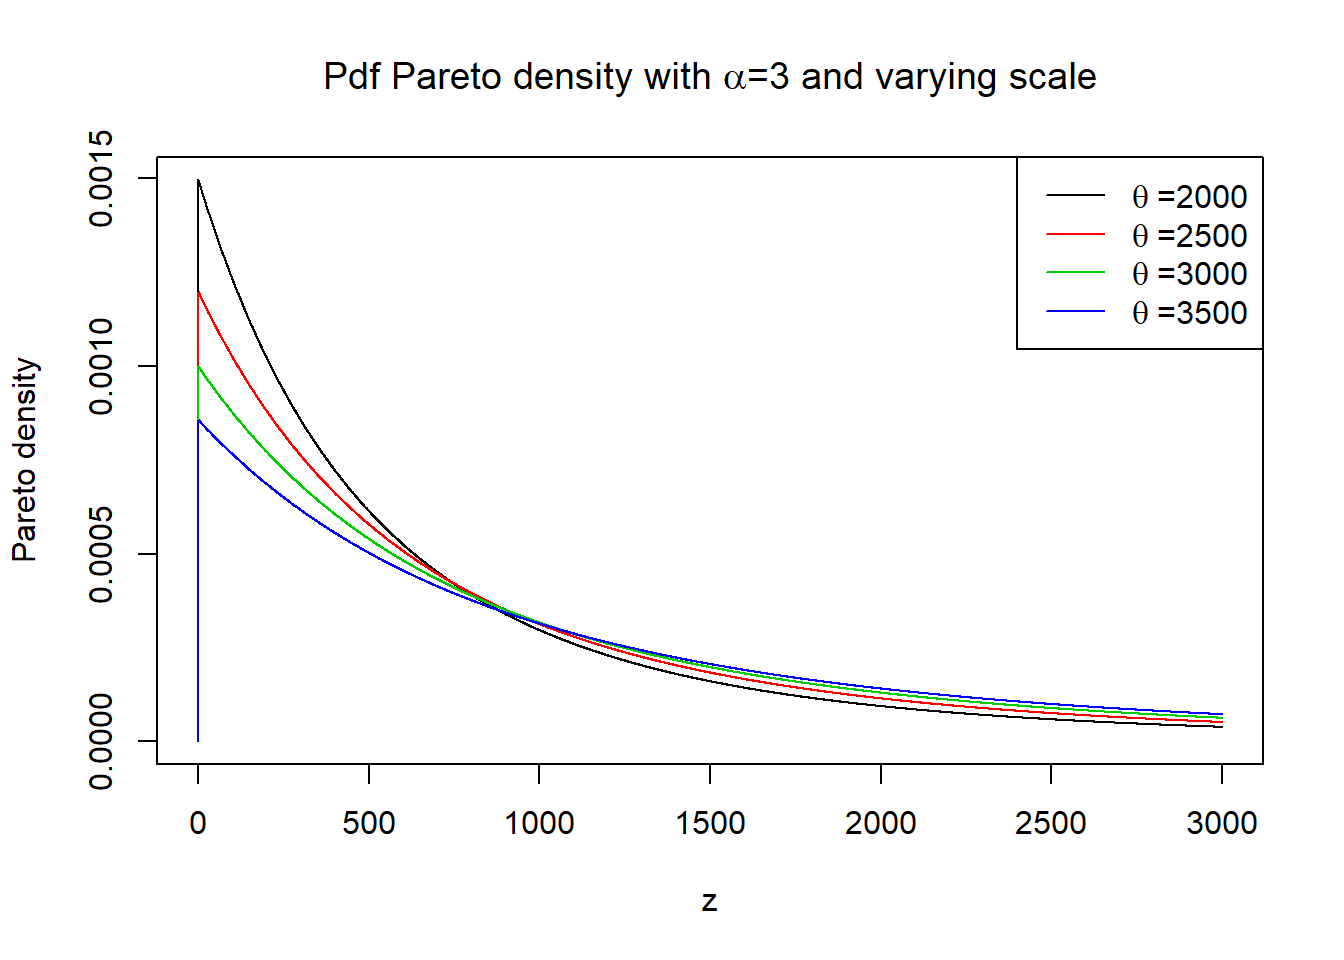
\includegraphics{R_for_Loss_Data_Analytics_files/figure-latex/unnamed-chunk-46-1} \end{center}

A few quick notes on these commands:

\begin{itemize}
\tightlist
\item
  The \texttt{coverage()} function computes probability density function
  or cumulative distribution function of the payment per payment or
  payment per loss random variable under any combination of the
  following coverage modifications: deductible, limit, coinsurance,
  inflation. In this illustration we used it to compute the probability
  density function of the payment per loss random variable with a
  deductible of 1.
\item
  The \texttt{f(0,\ 3)} function calculates the pdf when the payment per
  loss variable is 0 with gamma parameters shape=3 and rate=1. Because
  we used a deductible of 1 , this should be equal to
  \texttt{pgamma(0\ +\ 1,\ 3)}.
\end{itemize}

\subsubsection{Payment Per Payment with Ordinary
Deductible}\label{payment-per-payment-with-ordinary-deductible}

\(Y^P\) with pdf \(f_{Y^P}(y) = f_X(y+d)/S_X(d)\)

\begin{Shaded}
\begin{Highlighting}[]
\NormalTok{f <-}\StringTok{ }\KeywordTok{coverage}\NormalTok{(dgamma, pgamma, }\DataTypeTok{deductible =} \DecValTok{1}\NormalTok{)  }\CommentTok{# create the object}

\KeywordTok{f}\NormalTok{(}\DecValTok{0}\NormalTok{, }\DecValTok{3}\NormalTok{)  }\CommentTok{# calculate in x = 0, shape = 3, rate = 1}
\end{Highlighting}
\end{Shaded}

\begin{verbatim}
[1] 0
\end{verbatim}

\begin{Shaded}
\begin{Highlighting}[]
\KeywordTok{f}\NormalTok{(}\DecValTok{5}\NormalTok{, }\DecValTok{3}\NormalTok{)  }\CommentTok{# calculate in x = 5, shape = 3, rate = 1}
\end{Highlighting}
\end{Shaded}

\begin{verbatim}
[1] 0.04851322
\end{verbatim}

\begin{Shaded}
\begin{Highlighting}[]
\KeywordTok{dgamma}\NormalTok{(}\DecValTok{5} \OperatorTok{+}\StringTok{ }\DecValTok{1}\NormalTok{, }\DecValTok{3}\NormalTok{) }\OperatorTok{/}\StringTok{ }\KeywordTok{pgamma}\NormalTok{(}\DecValTok{1}\NormalTok{, }\DecValTok{3}\NormalTok{, }\DataTypeTok{lower =} \OtherTok{FALSE}\NormalTok{)  }\CommentTok{# DIY}
\end{Highlighting}
\end{Shaded}

\begin{verbatim}
[1] 0.04851322
\end{verbatim}

\begin{Shaded}
\begin{Highlighting}[]
\KeywordTok{curve}\NormalTok{(}\KeywordTok{dgamma}\NormalTok{(x, }\DecValTok{3}\NormalTok{), }\DataTypeTok{from =} \DecValTok{0}\NormalTok{, }\DataTypeTok{to =} \DecValTok{10}\NormalTok{, }\DataTypeTok{ylim =} \KeywordTok{c}\NormalTok{(}\DecValTok{0}\NormalTok{, }\FloatTok{0.3}\NormalTok{), }
      \DataTypeTok{lwd =} \DecValTok{1}\NormalTok{, }\DataTypeTok{col =} \StringTok{"gray"}\NormalTok{)  }\CommentTok{# original pdf}
\KeywordTok{curve}\NormalTok{(}\KeywordTok{dgamma}\NormalTok{(x, }\DecValTok{3}\NormalTok{), }\DataTypeTok{from =} \DecValTok{1}\NormalTok{, }\DataTypeTok{to =} \DecValTok{10}\NormalTok{, }\DataTypeTok{ylim =} \KeywordTok{c}\NormalTok{(}\DecValTok{0}\NormalTok{, }\FloatTok{0.3}\NormalTok{), }\DataTypeTok{add =} \OtherTok{TRUE}\NormalTok{, }\DataTypeTok{lwd =} \DecValTok{2}\NormalTok{) }
\KeywordTok{curve}\NormalTok{(}\KeywordTok{f}\NormalTok{(x, }\DecValTok{3}\NormalTok{), }\DataTypeTok{from =} \FloatTok{0.01}\NormalTok{, }\DataTypeTok{col =} \StringTok{"blue"}\NormalTok{, }
      \DataTypeTok{add =} \OtherTok{TRUE}\NormalTok{, }\DataTypeTok{lwd =} \DecValTok{2}\NormalTok{)     }\CommentTok{# modified pdf}
\KeywordTok{legend}\NormalTok{(}\StringTok{"topright"}\NormalTok{, }\KeywordTok{c}\NormalTok{(}\StringTok{"Original pdf"}\NormalTok{, }\StringTok{"Modified pdf"}\NormalTok{), }
       \DataTypeTok{lty =} \DecValTok{1}\NormalTok{, }\DataTypeTok{cex =} \FloatTok{0.6}\NormalTok{, }\DataTypeTok{col =} \KeywordTok{c}\NormalTok{(}\StringTok{"black"}\NormalTok{,}\StringTok{"blue"}\NormalTok{))}
\end{Highlighting}
\end{Shaded}

\begin{center}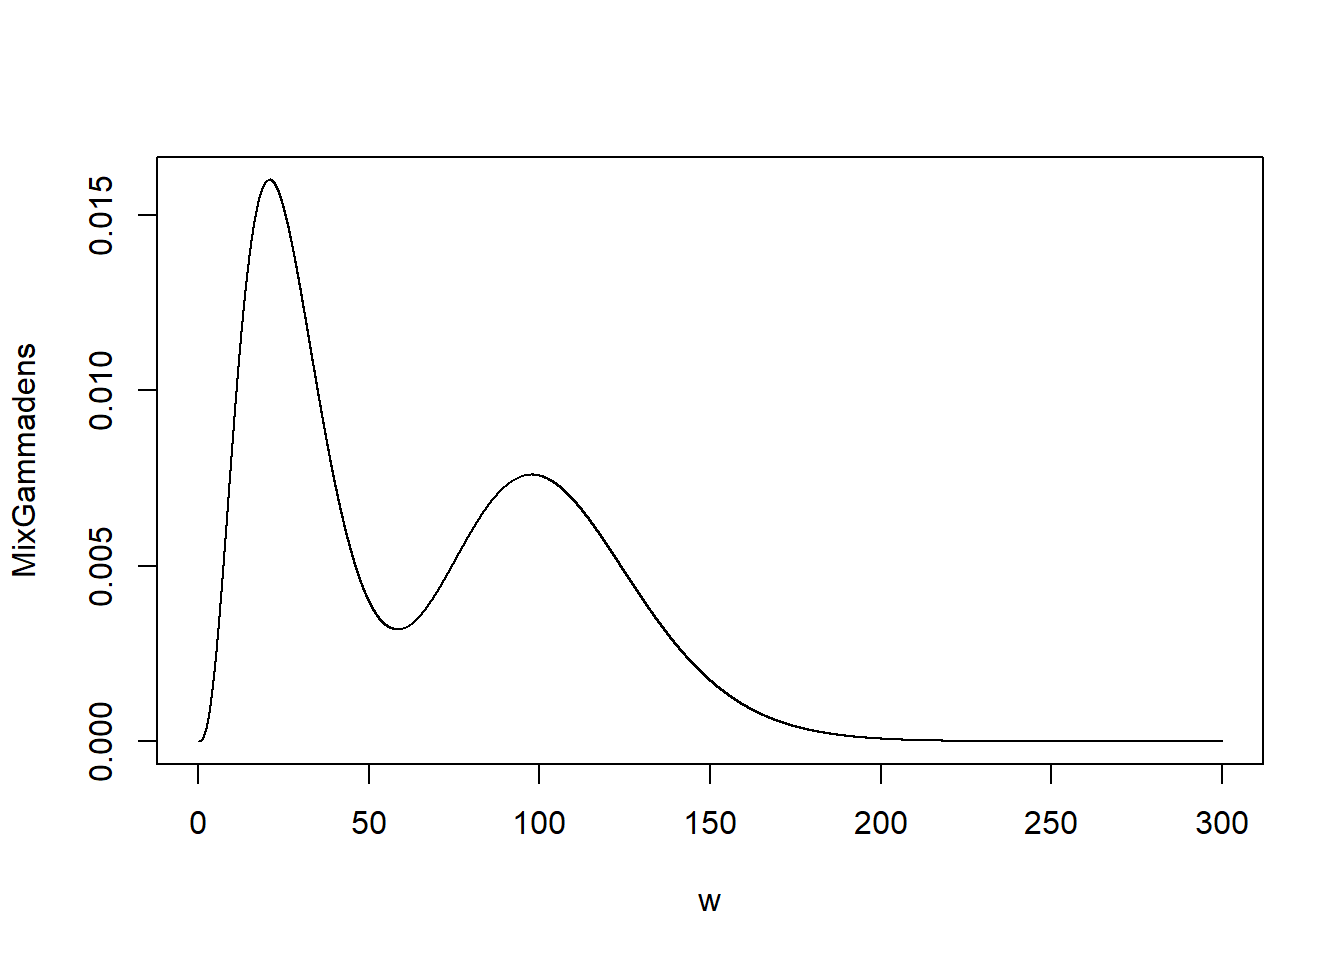
\includegraphics{R_for_Loss_Data_Analytics_files/figure-latex/unnamed-chunk-47-1} \end{center}

\subsubsection{Per Payment Variable with Policy Limit, Coinsurance and
Inflation}\label{per-payment-variable-with-policy-limit-coinsurance-and-inflation}

\begin{Shaded}
\begin{Highlighting}[]
\NormalTok{f <-}\StringTok{ }\KeywordTok{coverage}\NormalTok{(dgamma, pgamma, }\DataTypeTok{deductible =} \DecValTok{1}\NormalTok{, }\DataTypeTok{limit =} \DecValTok{100}\NormalTok{, }
              \DataTypeTok{coinsurance =} \FloatTok{0.9}\NormalTok{, }\DataTypeTok{inflation =} \FloatTok{0.05}\NormalTok{)  }
         \CommentTok{# create the object}

\KeywordTok{f}\NormalTok{(}\DecValTok{0}\NormalTok{, }\DecValTok{3}\NormalTok{)  }\CommentTok{# calculate in x = 0, shape = 3, rate = 1}
\end{Highlighting}
\end{Shaded}

\begin{verbatim}
[1] 0
\end{verbatim}

\begin{Shaded}
\begin{Highlighting}[]
\KeywordTok{f}\NormalTok{(}\DecValTok{5}\NormalTok{, }\DecValTok{3}\NormalTok{)  }\CommentTok{# calculate in x = 5, shape = 3, rate = 1}
\end{Highlighting}
\end{Shaded}

\begin{verbatim}
[1] 0.0431765
\end{verbatim}

\begin{Shaded}
\begin{Highlighting}[]
\KeywordTok{curve}\NormalTok{(}\KeywordTok{dgamma}\NormalTok{(x, }\DecValTok{3}\NormalTok{), }\DataTypeTok{from =} \DecValTok{0}\NormalTok{, }\DataTypeTok{to =} \DecValTok{10}\NormalTok{, }\DataTypeTok{ylim =} \KeywordTok{c}\NormalTok{(}\DecValTok{0}\NormalTok{, }\FloatTok{0.3}\NormalTok{), }
      \DataTypeTok{lwd =} \DecValTok{1}\NormalTok{, }\DataTypeTok{col =} \StringTok{"gray"}\NormalTok{)  }\CommentTok{# original pdf}
\KeywordTok{curve}\NormalTok{(}\KeywordTok{dgamma}\NormalTok{(x, }\DecValTok{3}\NormalTok{), }\DataTypeTok{from =} \DecValTok{1}\NormalTok{, }\DataTypeTok{to =} \DecValTok{10}\NormalTok{, }\DataTypeTok{ylim =} \KeywordTok{c}\NormalTok{(}\DecValTok{0}\NormalTok{, }\FloatTok{0.3}\NormalTok{), }\DataTypeTok{add =} \OtherTok{TRUE}\NormalTok{, }\DataTypeTok{lwd =} \DecValTok{2}\NormalTok{)}
\KeywordTok{curve}\NormalTok{(}\KeywordTok{f}\NormalTok{(x, }\DecValTok{3}\NormalTok{), }\DataTypeTok{from =} \FloatTok{0.01}\NormalTok{, }\DataTypeTok{col =} \StringTok{"blue"}\NormalTok{, }\DataTypeTok{add =} \OtherTok{TRUE}\NormalTok{, }\DataTypeTok{lwd =} \DecValTok{2}\NormalTok{)  }\CommentTok{# modified pdf}
\KeywordTok{legend}\NormalTok{(}\StringTok{"topright"}\NormalTok{, }\KeywordTok{c}\NormalTok{(}\StringTok{"Original pdf"}\NormalTok{, }\StringTok{"Modified pdf"}\NormalTok{), }
       \DataTypeTok{lty =} \DecValTok{1}\NormalTok{, }\DataTypeTok{cex =} \FloatTok{0.6}\NormalTok{, }\DataTypeTok{col =} \KeywordTok{c}\NormalTok{(}\StringTok{"black"}\NormalTok{, }\StringTok{"blue"}\NormalTok{))}
\end{Highlighting}
\end{Shaded}

\begin{center}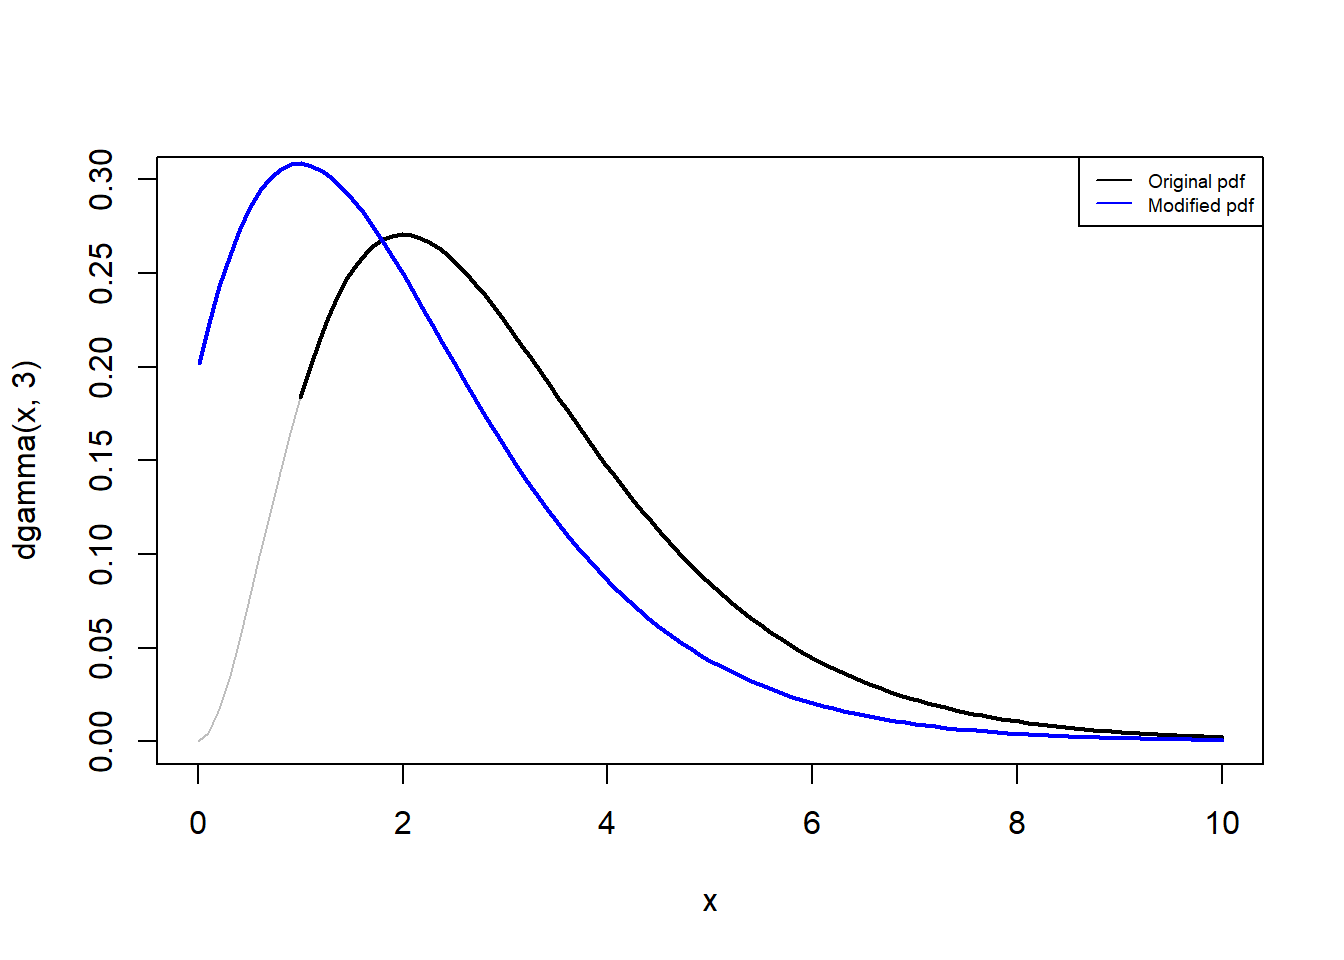
\includegraphics{R_for_Loss_Data_Analytics_files/figure-latex/unnamed-chunk-48-1} \end{center}

\subsection{Franchise Deductible}\label{franchise-deductible}

A policy with a \emph{franchise deductible} of \(d\) pays nothing if the
loss is no greater than \(d\), and pays the full amount of the loss if
it is greater than \(d\). This section plots the pdf for the per payment
and per loss random variable.

\subsubsection{Payment Per Loss with Franchise
Deductible}\label{payment-per-loss-with-franchise-deductible}

\begin{Shaded}
\begin{Highlighting}[]
\CommentTok{# Franchise deductible }
\CommentTok{# Per loss variable}
\NormalTok{f <-}\StringTok{ }\KeywordTok{coverage}\NormalTok{(dgamma, pgamma, }\DataTypeTok{deductible =} \DecValTok{1}\NormalTok{, }\DataTypeTok{per.loss =} \OtherTok{TRUE}\NormalTok{, }\DataTypeTok{franchise =} \OtherTok{TRUE}\NormalTok{)}
\KeywordTok{f}\NormalTok{(}\DecValTok{0}\NormalTok{, }\DecValTok{3}\NormalTok{)  }\CommentTok{# mass at 0}
\end{Highlighting}
\end{Shaded}

\begin{verbatim}
[1] 0.0803014
\end{verbatim}

\begin{Shaded}
\begin{Highlighting}[]
\KeywordTok{pgamma}\NormalTok{(}\DecValTok{1}\NormalTok{, }\DecValTok{3}\NormalTok{)  }\CommentTok{# idem}
\end{Highlighting}
\end{Shaded}

\begin{verbatim}
[1] 0.0803014
\end{verbatim}

\begin{Shaded}
\begin{Highlighting}[]
\KeywordTok{f}\NormalTok{(}\FloatTok{0.5}\NormalTok{, }\DecValTok{3}\NormalTok{)  }\CommentTok{# 0 < x < 1}
\end{Highlighting}
\end{Shaded}

\begin{verbatim}
[1] 0
\end{verbatim}

\begin{Shaded}
\begin{Highlighting}[]
\KeywordTok{f}\NormalTok{(}\DecValTok{1}\NormalTok{, }\DecValTok{3}\NormalTok{)  }\CommentTok{# x = 1}
\end{Highlighting}
\end{Shaded}

\begin{verbatim}
[1] 0
\end{verbatim}

\begin{Shaded}
\begin{Highlighting}[]
\KeywordTok{f}\NormalTok{(}\DecValTok{5}\NormalTok{, }\DecValTok{3}\NormalTok{)  }\CommentTok{# x > 1}
\end{Highlighting}
\end{Shaded}

\begin{verbatim}
[1] 0.08422434
\end{verbatim}

\begin{Shaded}
\begin{Highlighting}[]
\KeywordTok{dgamma}\NormalTok{(}\DecValTok{5}\NormalTok{, }\DecValTok{3}\NormalTok{)}
\end{Highlighting}
\end{Shaded}

\begin{verbatim}
[1] 0.08422434
\end{verbatim}

\begin{Shaded}
\begin{Highlighting}[]
\KeywordTok{curve}\NormalTok{(}\KeywordTok{dgamma}\NormalTok{(x, }\DecValTok{3}\NormalTok{), }\DataTypeTok{from =} \DecValTok{0}\NormalTok{, }\DataTypeTok{to =} \DecValTok{10}\NormalTok{, }\DataTypeTok{ylim =} \KeywordTok{c}\NormalTok{(}\DecValTok{0}\NormalTok{, }\FloatTok{0.3}\NormalTok{))  }\CommentTok{# original}
\KeywordTok{curve}\NormalTok{(}\KeywordTok{f}\NormalTok{(x, }\DecValTok{3}\NormalTok{), }\DataTypeTok{from =} \FloatTok{1.1}\NormalTok{, }\DataTypeTok{col =} \StringTok{"blue"}\NormalTok{, }\DataTypeTok{add =} \OtherTok{TRUE}\NormalTok{)  }\CommentTok{# modified}
\KeywordTok{points}\NormalTok{(}\DecValTok{0}\NormalTok{, }\KeywordTok{f}\NormalTok{(}\DecValTok{0}\NormalTok{, }\DecValTok{3}\NormalTok{), }\DataTypeTok{pch =} \DecValTok{16}\NormalTok{, }\DataTypeTok{col =} \StringTok{"blue"}\NormalTok{)  }\CommentTok{# mass at 0}
\KeywordTok{curve}\NormalTok{(}\KeywordTok{f}\NormalTok{(x, }\DecValTok{3}\NormalTok{), }\DataTypeTok{from =} \FloatTok{0.1}\NormalTok{, }\DataTypeTok{to =} \DecValTok{1}\NormalTok{, }\DataTypeTok{col =} \StringTok{"blue"}\NormalTok{, }\DataTypeTok{add =} \OtherTok{TRUE}\NormalTok{)  }\CommentTok{# 0 < x < 1}
\KeywordTok{legend}\NormalTok{(}\StringTok{"topright"}\NormalTok{, }\KeywordTok{c}\NormalTok{(}\StringTok{"Original pdf"}\NormalTok{, }\StringTok{"Modified pdf"}\NormalTok{), }
       \DataTypeTok{lty =} \DecValTok{1}\NormalTok{, }\DataTypeTok{cex =} \FloatTok{0.6}\NormalTok{, }\DataTypeTok{col =} \KeywordTok{c}\NormalTok{(}\StringTok{"black"}\NormalTok{, }\StringTok{"blue"}\NormalTok{))}
\end{Highlighting}
\end{Shaded}

\begin{center}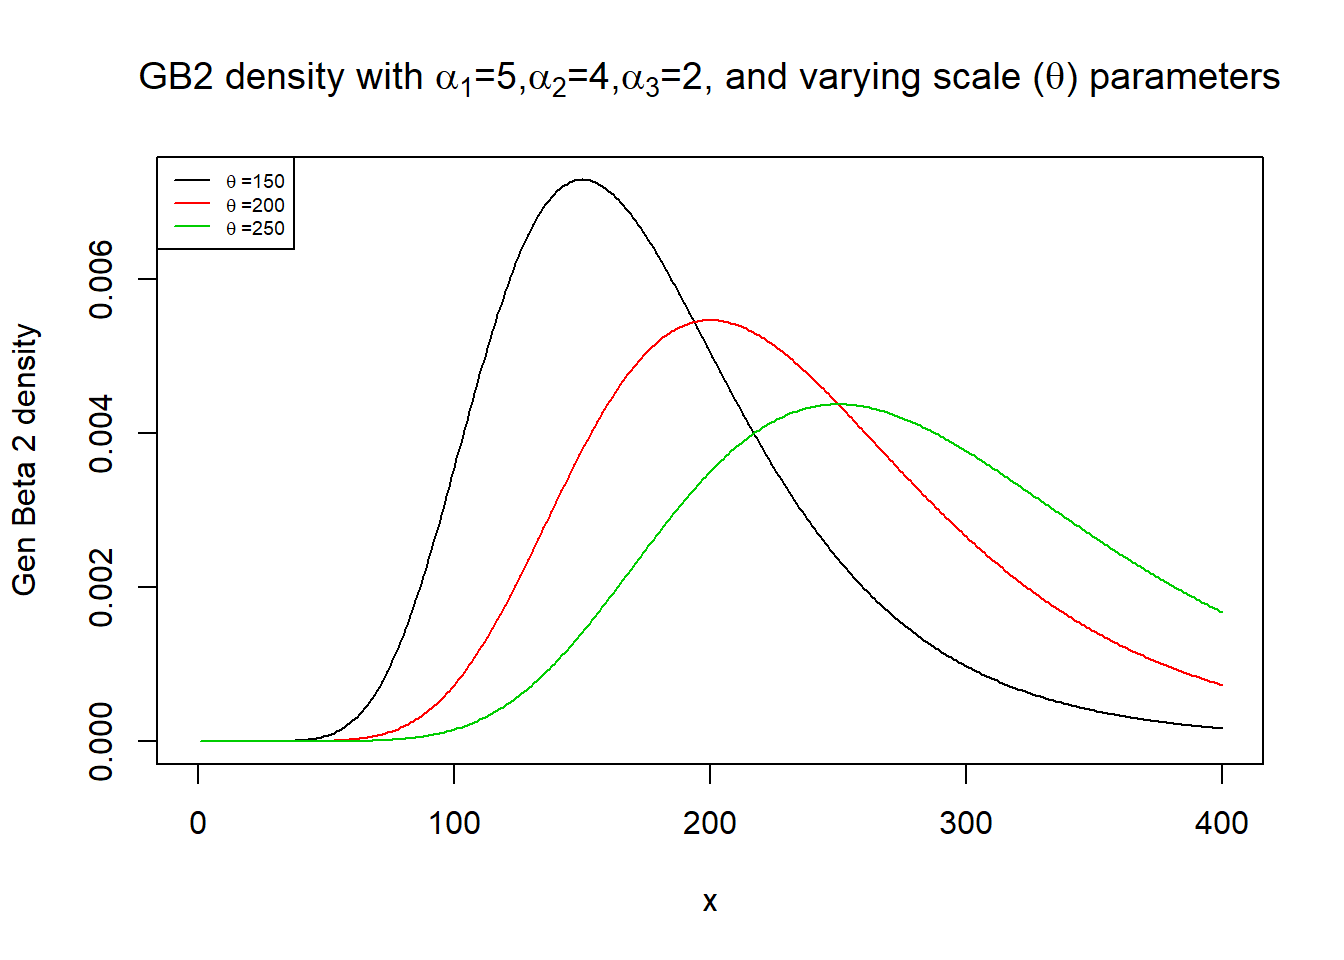
\includegraphics{R_for_Loss_Data_Analytics_files/figure-latex/unnamed-chunk-49-1} \end{center}

Note : To use the franchise deductible , we have to add the option
\texttt{franchise\ =\ TRUE} in the coverage function.

\subsubsection{Payment Per Payment with Franchise
Deductible}\label{payment-per-payment-with-franchise-deductible}

\begin{Shaded}
\begin{Highlighting}[]
\CommentTok{# Franchise deductible}
\CommentTok{# Per payment variable}
\NormalTok{f <-}\StringTok{ }\KeywordTok{coverage}\NormalTok{(dgamma, pgamma, }\DataTypeTok{deductible =} \DecValTok{1}\NormalTok{, }\DataTypeTok{franchise =} \OtherTok{TRUE}\NormalTok{)}
\KeywordTok{f}\NormalTok{(}\DecValTok{0}\NormalTok{, }\DecValTok{3}\NormalTok{)  }\CommentTok{# x = 0}
\end{Highlighting}
\end{Shaded}

\begin{verbatim}
[1] 0
\end{verbatim}

\begin{Shaded}
\begin{Highlighting}[]
\KeywordTok{f}\NormalTok{(}\FloatTok{0.5}\NormalTok{, }\DecValTok{3}\NormalTok{)  }\CommentTok{# 0 < x < 1}
\end{Highlighting}
\end{Shaded}

\begin{verbatim}
[1] 0
\end{verbatim}

\begin{Shaded}
\begin{Highlighting}[]
\KeywordTok{f}\NormalTok{(}\DecValTok{1}\NormalTok{, }\DecValTok{3}\NormalTok{)  }\CommentTok{# x = 1}
\end{Highlighting}
\end{Shaded}

\begin{verbatim}
[1] 0
\end{verbatim}

\begin{Shaded}
\begin{Highlighting}[]
\KeywordTok{f}\NormalTok{(}\DecValTok{5}\NormalTok{, }\DecValTok{3}\NormalTok{)  }\CommentTok{# x > 1}
\end{Highlighting}
\end{Shaded}

\begin{verbatim}
[1] 0.09157819
\end{verbatim}

\begin{Shaded}
\begin{Highlighting}[]
\KeywordTok{dgamma}\NormalTok{(}\DecValTok{5}\NormalTok{, }\DecValTok{3}\NormalTok{) }\OperatorTok{/}\StringTok{ }\KeywordTok{pgamma}\NormalTok{(}\DecValTok{1}\NormalTok{, }\DecValTok{3}\NormalTok{, }\DataTypeTok{lower =} \OtherTok{FALSE}\NormalTok{)  }\CommentTok{# idem}
\end{Highlighting}
\end{Shaded}

\begin{verbatim}
[1] 0.09157819
\end{verbatim}

\begin{Shaded}
\begin{Highlighting}[]
\KeywordTok{curve}\NormalTok{(}\KeywordTok{dgamma}\NormalTok{(x, }\DecValTok{3}\NormalTok{), }\DataTypeTok{from =} \DecValTok{0}\NormalTok{, }\DataTypeTok{to =} \DecValTok{10}\NormalTok{, }\DataTypeTok{ylim =} \KeywordTok{c}\NormalTok{(}\DecValTok{0}\NormalTok{, }\FloatTok{0.3}\NormalTok{))  }\CommentTok{# original}
\KeywordTok{curve}\NormalTok{(}\KeywordTok{f}\NormalTok{(x, }\DecValTok{3}\NormalTok{), }\DataTypeTok{from =} \FloatTok{1.1}\NormalTok{, }\DataTypeTok{col =} \StringTok{"blue"}\NormalTok{, }\DataTypeTok{add =} \OtherTok{TRUE}\NormalTok{)  }\CommentTok{# modified}
\KeywordTok{curve}\NormalTok{(}\KeywordTok{f}\NormalTok{(x, }\DecValTok{3}\NormalTok{), }\DataTypeTok{from =} \DecValTok{0}\NormalTok{, }\DataTypeTok{to =} \DecValTok{1}\NormalTok{, }\DataTypeTok{col =} \StringTok{"blue"}\NormalTok{, }\DataTypeTok{add =} \OtherTok{TRUE}\NormalTok{)  }\CommentTok{# 0 < x < 1}
\KeywordTok{legend}\NormalTok{(}\StringTok{"topright"}\NormalTok{, }\KeywordTok{c}\NormalTok{(}\StringTok{"Original pdf"}\NormalTok{, }\StringTok{"Modified pdf"}\NormalTok{), }
       \DataTypeTok{lty =} \DecValTok{1}\NormalTok{, }\DataTypeTok{cex =} \FloatTok{0.6}\NormalTok{, }\DataTypeTok{col =} \KeywordTok{c}\NormalTok{(}\StringTok{"black"}\NormalTok{, }\StringTok{"blue"}\NormalTok{))}
\end{Highlighting}
\end{Shaded}

\begin{center}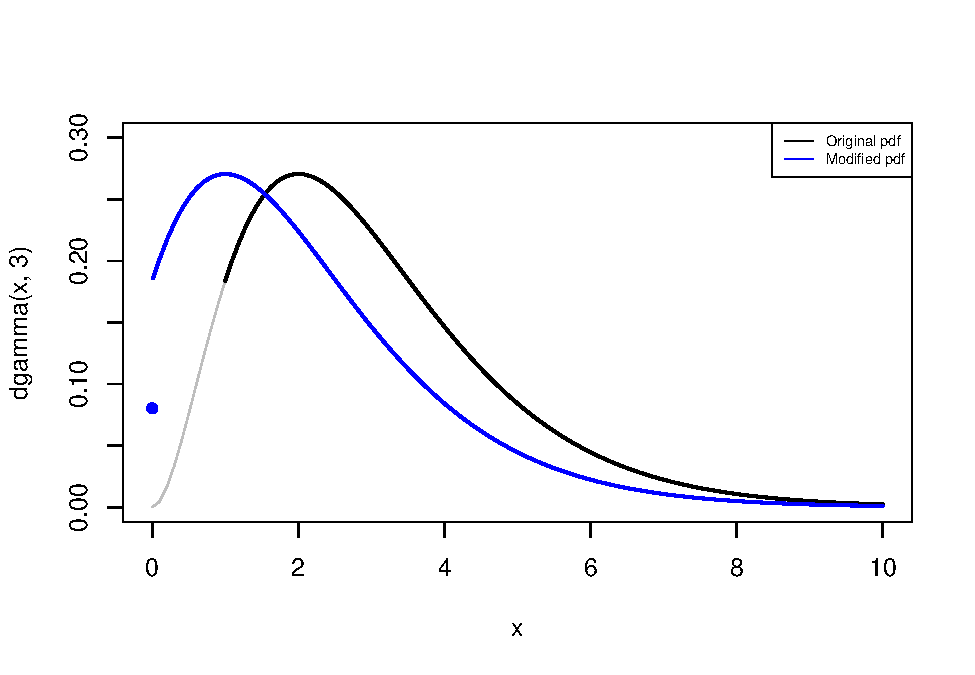
\includegraphics{R_for_Loss_Data_Analytics_files/figure-latex/unnamed-chunk-50-1} \end{center}

\chapter{Model Selection}\label{model-selection}

\emph{This file contains illustrative \textbf{R} code for computing
important count distributions. When reviewing this code, you should open
an \textbf{R} session, copy-and-paste the code, and see it perform.
Then, you will be able to change parameters, look up commands, and so
forth, as you go.This code uses the dataset \texttt{CLAIMLEVEL.csv} }

\section{Claim Level Data of Property
Fund}\label{claim-level-data-of-property-fund}

This section summarizes claims from the property fund for year 2010 and
plots the data.

\subsection{Claims Data}\label{claims-data}

The results below considers individual claims from the property fund for
year 2010.

\begin{Shaded}
\begin{Highlighting}[]
\NormalTok{## Read in data and get number of claims.  }
\NormalTok{claim_lev <-}\StringTok{ }\KeywordTok{read.csv}\NormalTok{(}\StringTok{"Data/CLAIMLEVEL.csv"}\NormalTok{, }\DataTypeTok{header =} \OtherTok{TRUE}\NormalTok{) }
\KeywordTok{nrow}\NormalTok{(claim_lev)  }\CommentTok{# 6258}
\end{Highlighting}
\end{Shaded}

\begin{verbatim}
[1] 6258
\end{verbatim}

\begin{Shaded}
\begin{Highlighting}[]
\CommentTok{# 2010 subset }
\NormalTok{claim_data <-}\StringTok{ }\KeywordTok{subset}\NormalTok{(claim_lev, Year }\OperatorTok{==}\StringTok{ }\DecValTok{2010}\NormalTok{); }
\KeywordTok{length}\NormalTok{(}\KeywordTok{unique}\NormalTok{(claim_data}\OperatorTok{$}\NormalTok{PolicyNum))  }\CommentTok{# 403 unique policyholders}
\end{Highlighting}
\end{Shaded}

\begin{verbatim}
[1] 403
\end{verbatim}

\begin{Shaded}
\begin{Highlighting}[]
\NormalTok{n_tot <-}\StringTok{ }\KeywordTok{nrow}\NormalTok{(claim_data)  }\CommentTok{# 1377 individual claims}
\NormalTok{n_tot}
\end{Highlighting}
\end{Shaded}

\begin{verbatim}
[1] 1377
\end{verbatim}

\begin{Shaded}
\begin{Highlighting}[]
\CommentTok{# As an alternative, you can simulate claims}
\CommentTok{# n_tot <- 13770}
\CommentTok{# alpha_hat <- 2}
\CommentTok{# theta_hat <- 100}
\CommentTok{# claim <- rgamma(n_tot, shape = alpha_hat, scale = theta_hat)}
\CommentTok{# claim <- rparetoII(n_tot, loc = 0,  shape = alpha_hat, scale = theta_hat)}
\CommentTok{# GB2}
\CommentTok{# claim <- theta_hat * rgamma(n_tot, shape = alpha_hat, scale = 1) / }
\CommentTok{#          rgamma(n_tot, shape = 1, scale = 1) }
\CommentTok{# claim_data <- data.frame(claim)}

\NormalTok{###################################################}
\end{Highlighting}
\end{Shaded}

\subsection{Summary of Claims}\label{summary-of-claims}

The output below provides summary on claims data for 2010 and summary in
logarithmic units.

\begin{Shaded}
\begin{Highlighting}[]
\CommentTok{# Summarizing the claim data for 2010}
\KeywordTok{summary}\NormalTok{(claim_data}\OperatorTok{$}\NormalTok{Claim)}
\end{Highlighting}
\end{Shaded}

\begin{verbatim}
    Min.  1st Qu.   Median     Mean  3rd Qu.     Max. 
       1      789     2250    26623     6171 12922218 
\end{verbatim}

\begin{Shaded}
\begin{Highlighting}[]
\KeywordTok{sd}\NormalTok{(claim_data}\OperatorTok{$}\NormalTok{Claim)}
\end{Highlighting}
\end{Shaded}

\begin{verbatim}
[1] 368029.7
\end{verbatim}

\begin{Shaded}
\begin{Highlighting}[]
\CommentTok{# Summarizing logarithmic claims for 2010}
\KeywordTok{summary}\NormalTok{(}\KeywordTok{log}\NormalTok{(claim_data}\OperatorTok{$}\NormalTok{Claim))}
\end{Highlighting}
\end{Shaded}

\begin{verbatim}
   Min. 1st Qu.  Median    Mean 3rd Qu.    Max. 
  0.000   6.670   7.719   7.804   8.728  16.374 
\end{verbatim}

\begin{Shaded}
\begin{Highlighting}[]
\KeywordTok{sd}\NormalTok{(}\KeywordTok{log}\NormalTok{(claim_data}\OperatorTok{$}\NormalTok{Claim))}
\end{Highlighting}
\end{Shaded}

\begin{verbatim}
[1] 1.683297
\end{verbatim}

\subsection{Plot of Claims}\label{plot-of-claims}

The plots below provides further information about the distribution of
sample claims.

\begin{Shaded}
\begin{Highlighting}[]
\CommentTok{# Histogram }
\KeywordTok{par}\NormalTok{(}\DataTypeTok{mfrow =} \KeywordTok{c}\NormalTok{(}\DecValTok{1}\NormalTok{, }\DecValTok{2}\NormalTok{))}
\KeywordTok{hist}\NormalTok{(claim_data}\OperatorTok{$}\NormalTok{Claim, }\DataTypeTok{main=}\StringTok{""}\NormalTok{, }\DataTypeTok{xlab =} \StringTok{"Claims"}\NormalTok{)}
\KeywordTok{hist}\NormalTok{(}\KeywordTok{log}\NormalTok{(claim_data}\OperatorTok{$}\NormalTok{Claim), }\DataTypeTok{main =} \StringTok{""}\NormalTok{, }\DataTypeTok{xlab =} \StringTok{"Logarithmic Claims"}\NormalTok{)}
\end{Highlighting}
\end{Shaded}

\begin{center}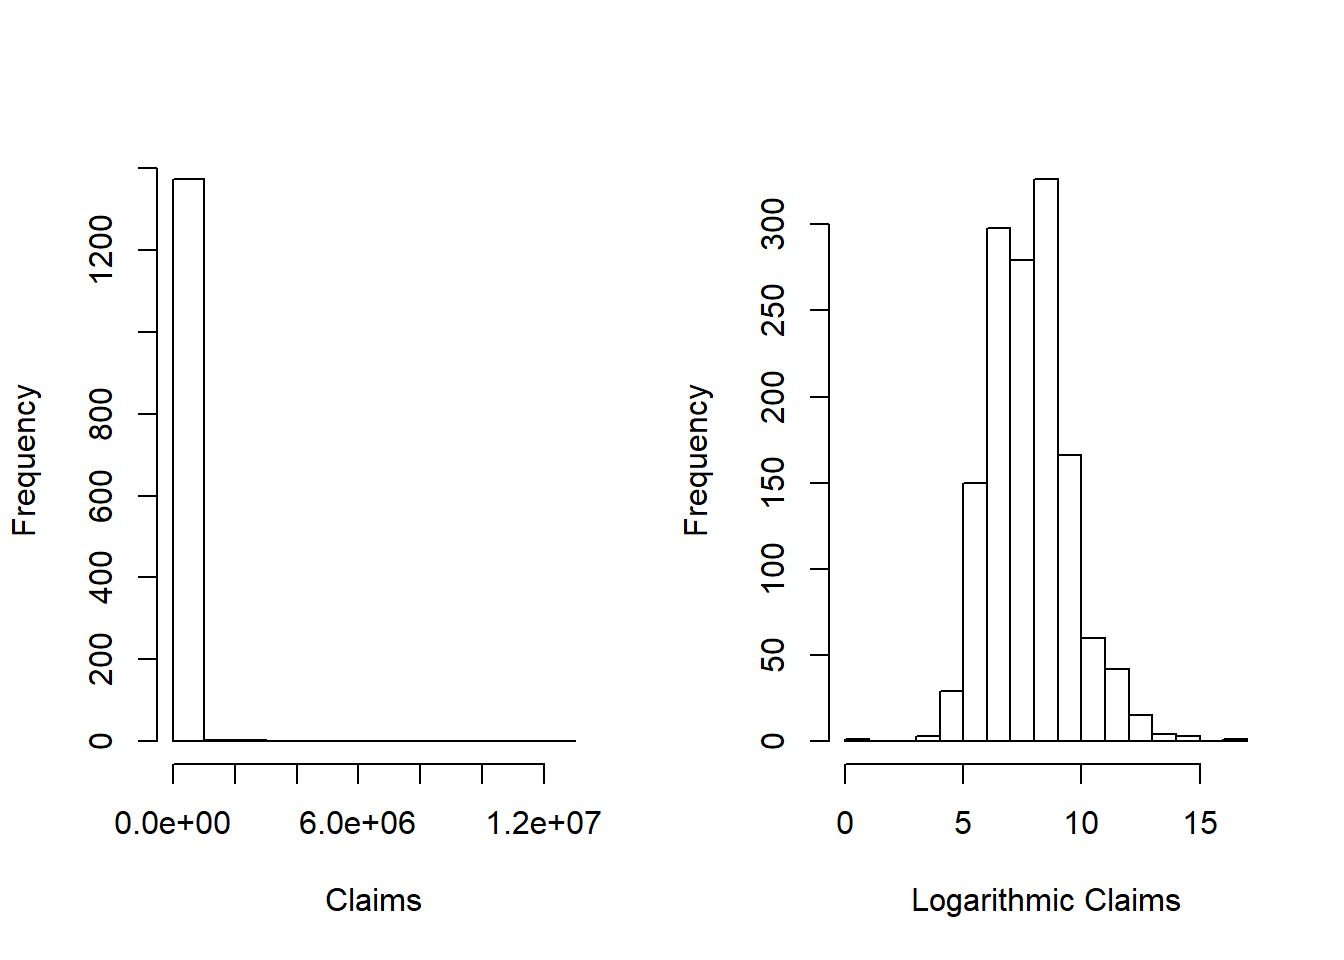
\includegraphics{R_for_Loss_Data_Analytics_files/figure-latex/unnamed-chunk-53-1} \end{center}

\begin{Shaded}
\begin{Highlighting}[]
\CommentTok{# dev.off()}
\end{Highlighting}
\end{Shaded}

\section{Fitting Distributions}\label{fitting-distributions}

This section shows how to fit basic distributions to a data set.

\subsection{Inference Assuming a Lognormal
Distribution}\label{inference-assuming-a-lognormal-distribution}

The results below assume that the data follow a lognormal distribution
and uses\texttt{VGAM} library for estimation of parameters.

\begin{Shaded}
\begin{Highlighting}[]
\CommentTok{# Inference assuming a lognormal distribution}
\CommentTok{# First, take the log of the data and assume normality}
\NormalTok{y <-}\StringTok{ }\KeywordTok{log}\NormalTok{(claim_data}\OperatorTok{$}\NormalTok{Claim)}
\KeywordTok{summary}\NormalTok{(y)}
\end{Highlighting}
\end{Shaded}

\begin{verbatim}
   Min. 1st Qu.  Median    Mean 3rd Qu.    Max. 
  0.000   6.670   7.719   7.804   8.728  16.374 
\end{verbatim}

\begin{Shaded}
\begin{Highlighting}[]
\KeywordTok{sd}\NormalTok{(y)}
\end{Highlighting}
\end{Shaded}

\begin{verbatim}
[1] 1.683297
\end{verbatim}

\begin{Shaded}
\begin{Highlighting}[]
\CommentTok{# Confidence intervals and hypothesis test}
\KeywordTok{t.test}\NormalTok{(y, }\DataTypeTok{mu =} \KeywordTok{log}\NormalTok{(}\DecValTok{5000}\NormalTok{))  }\CommentTok{# H0: mu_o = log(5000) = 8.517}
\end{Highlighting}
\end{Shaded}

\begin{verbatim}

    One Sample t-test

data:  y
t = -15.717, df = 1376, p-value < 2.2e-16
alternative hypothesis: true mean is not equal to 8.517193
95 percent confidence interval:
 7.715235 7.893208
sample estimates:
mean of x 
 7.804222 
\end{verbatim}

\begin{Shaded}
\begin{Highlighting}[]
\CommentTok{# Mean of the lognormal distribution}
\KeywordTok{exp}\NormalTok{(}\KeywordTok{mean}\NormalTok{(y) }\OperatorTok{+}\StringTok{ }\KeywordTok{sd}\NormalTok{(y)}\OperatorTok{^}\DecValTok{2} \OperatorTok{/}\StringTok{ }\DecValTok{2}\NormalTok{)}
\end{Highlighting}
\end{Shaded}

\begin{verbatim}
[1] 10106.82
\end{verbatim}

\begin{Shaded}
\begin{Highlighting}[]
\KeywordTok{mean}\NormalTok{(claim_data}\OperatorTok{$}\NormalTok{Claim)}
\end{Highlighting}
\end{Shaded}

\begin{verbatim}
[1] 26622.59
\end{verbatim}

\begin{Shaded}
\begin{Highlighting}[]
\CommentTok{# Alternatively, assume that the data follow a lognormal distribution}
\CommentTok{# Use "VGAM" library for estimation of parameters }
\KeywordTok{library}\NormalTok{(VGAM)}
\NormalTok{fit.LN <-}\StringTok{ }\KeywordTok{vglm}\NormalTok{(Claim }\OperatorTok{~}\StringTok{ }\DecValTok{1}\NormalTok{, }\DataTypeTok{family =}\NormalTok{ lognormal, }\DataTypeTok{data =}\NormalTok{ claim_data)}
\KeywordTok{summary}\NormalTok{(fit.LN)}
\end{Highlighting}
\end{Shaded}

\begin{verbatim}

Call:
vglm(formula = Claim ~ 1, family = lognormal, data = claim_data)


Pearson residuals:
                Min      1Q   Median     3Q    Max
meanlog     -4.6380 -0.6740 -0.05083 0.5487  5.093
loge(sdlog) -0.7071 -0.6472 -0.44003 0.1135 17.636

Coefficients: 
              Estimate Std. Error z value Pr(>|z|)    
(Intercept):1  7.80422    0.04535  172.10   <2e-16 ***
(Intercept):2  0.52039    0.01906   27.31   <2e-16 ***
---
Signif. codes:  0 '***' 0.001 '**' 0.01 '*' 0.05 '.' 0.1 ' ' 1

Number of linear predictors:  2 

Names of linear predictors: meanlog, loge(sdlog)

Log-likelihood: -13416.87 on 2752 degrees of freedom

Number of iterations: 3 

No Hauck-Donner effect found in any of the estimates
\end{verbatim}

\begin{Shaded}
\begin{Highlighting}[]
\KeywordTok{coef}\NormalTok{(fit.LN)                   }\CommentTok{# coefficients}
\end{Highlighting}
\end{Shaded}

\begin{verbatim}
(Intercept):1 (Intercept):2 
    7.8042218     0.5203908 
\end{verbatim}

\begin{Shaded}
\begin{Highlighting}[]
\KeywordTok{confint}\NormalTok{(fit.LN, }\DataTypeTok{level =} \FloatTok{0.95}\NormalTok{)  }\CommentTok{# confidence intervals for model parameters }
\end{Highlighting}
\end{Shaded}

\begin{verbatim}
                  2.5 %    97.5 %
(Intercept):1 7.7153457 7.8930978
(Intercept):2 0.4830429 0.5577387
\end{verbatim}

\begin{Shaded}
\begin{Highlighting}[]
\KeywordTok{logLik}\NormalTok{(fit.LN)                 }\CommentTok{# loglikelihood for lognormal}
\end{Highlighting}
\end{Shaded}

\begin{verbatim}
[1] -13416.87
\end{verbatim}

\begin{Shaded}
\begin{Highlighting}[]
\KeywordTok{AIC}\NormalTok{(fit.LN)                    }\CommentTok{# AIC for lognormal}
\end{Highlighting}
\end{Shaded}

\begin{verbatim}
[1] 26837.74
\end{verbatim}

\begin{Shaded}
\begin{Highlighting}[]
\KeywordTok{BIC}\NormalTok{(fit.LN)                    }\CommentTok{# BIC for lognormal}
\end{Highlighting}
\end{Shaded}

\begin{verbatim}
[1] 26848.2
\end{verbatim}

\begin{Shaded}
\begin{Highlighting}[]
\KeywordTok{vcov}\NormalTok{(fit.LN)                   }\CommentTok{# covariance matrix for model parameters }
\end{Highlighting}
\end{Shaded}

\begin{verbatim}
              (Intercept):1 (Intercept):2
(Intercept):1   0.002056237  0.0000000000
(Intercept):2   0.000000000  0.0003631082
\end{verbatim}

\begin{Shaded}
\begin{Highlighting}[]
\CommentTok{# Mean of the lognormal distribution}
\KeywordTok{exp}\NormalTok{(}\KeywordTok{mean}\NormalTok{(y) }\OperatorTok{+}\StringTok{ }\KeywordTok{sd}\NormalTok{(y)}\OperatorTok{^}\DecValTok{2} \OperatorTok{/}\StringTok{ }\DecValTok{2}\NormalTok{)}
\end{Highlighting}
\end{Shaded}

\begin{verbatim}
[1] 10106.82
\end{verbatim}

\begin{Shaded}
\begin{Highlighting}[]
\KeywordTok{exp}\NormalTok{(}\KeywordTok{coef}\NormalTok{(fit.LN))}
\end{Highlighting}
\end{Shaded}

\begin{verbatim}
(Intercept):1 (Intercept):2 
  2450.927448      1.682685 
\end{verbatim}

A few quick notes on these commands:

\begin{itemize}
\tightlist
\item
  The \texttt{t.test()} function can be used for a variety of t-tests.
  In this illustration, it was used to test
  \(H_0=\mu_0=\log(5000)=8.517\).
\item
  The \texttt{vglm()} function is used to fit vector generalized linear
  models (VGLMs). See \texttt{help(vglm)} for other modeling options.
\item
  The \texttt{coef()} function returns the estimated coefficients from
  the \texttt{vglm} or other modeling functions.
\item
  The \texttt{confint} function provides the confidence intervals for
  model parameters.
\item
  The \texttt{loglik} function provides the log-likelihood value for the
  lognormal estimation from the \texttt{vglm} or other modeling
  functions.
\item
  \texttt{AIC()} and \texttt{BIC()} returns Akaike's Information
  Criterion and BIC or SBC (Schwarz's Bayesian criterion) for the fitted
  lognormal model.
  \(\text{AIC} =-2* \text{(loglikelihood)} + 2*\text{npar}\) , where
  \texttt{npar} represents the number of parameters in the fitted model,
  and \(\text{BIC} =-2* \text{log-likelihood} + \log(n)* \text{npar}\)
  where \(n\) is the number of observations.
\item
  \texttt{vcov()} returns the covariance matrix for model parameters.
\end{itemize}

\subsection{Inference Assuming a Gamma
Distribution}\label{inference-assuming-a-gamma-distribution}

The results below assume that the data follow a gamma distribution and
uses\texttt{VGAM} library for estimation of parameters.

\begin{Shaded}
\begin{Highlighting}[]
\CommentTok{# Inference assuming a gamma distribution}
\CommentTok{# Install.packages("VGAM")}
\KeywordTok{library}\NormalTok{(VGAM)}
\NormalTok{fit.gamma <-}\StringTok{ }\KeywordTok{vglm}\NormalTok{(Claim }\OperatorTok{~}\StringTok{ }\DecValTok{1}\NormalTok{, }\DataTypeTok{family =}\NormalTok{ gamma2, }\DataTypeTok{data =}\NormalTok{ claim_data)}
\KeywordTok{summary}\NormalTok{(fit.gamma)}
\end{Highlighting}
\end{Shaded}

\begin{verbatim}

Call:
vglm(formula = Claim ~ 1, family = gamma2, data = claim_data)


Pearson residuals:
                 Min      1Q  Median      3Q     Max
loge(mu)      -0.539 -0.5231 -0.4935 -0.4141 261.117
loge(shape) -153.990 -0.1024  0.2335  0.4969   0.772

Coefficients: 
              Estimate Std. Error z value Pr(>|z|)    
(Intercept):1 10.18952    0.04999  203.82   <2e-16 ***
(Intercept):2 -1.23582    0.03001  -41.17   <2e-16 ***
---
Signif. codes:  0 '***' 0.001 '**' 0.01 '*' 0.05 '.' 0.1 ' ' 1

Number of linear predictors:  2 

Names of linear predictors: loge(mu), loge(shape)

Log-likelihood: -14150.59 on 2752 degrees of freedom

Number of iterations: 13 

No Hauck-Donner effect found in any of the estimates
\end{verbatim}

\begin{Shaded}
\begin{Highlighting}[]
\KeywordTok{coef}\NormalTok{(fit.gamma)                 }\CommentTok{# This uses a different parameterization }
\end{Highlighting}
\end{Shaded}

\begin{verbatim}
(Intercept):1 (Intercept):2 
    10.189515     -1.235822 
\end{verbatim}

\begin{Shaded}
\begin{Highlighting}[]
\NormalTok{( theta <-}\StringTok{ }\KeywordTok{exp}\NormalTok{(}\KeywordTok{coef}\NormalTok{(fit.gamma)[}\DecValTok{1}\NormalTok{]) }\OperatorTok{/}\StringTok{ }\KeywordTok{exp}\NormalTok{(}\KeywordTok{coef}\NormalTok{(fit.gamma)[}\DecValTok{2}\NormalTok{]) )  }\CommentTok{# theta = mu / alpha}
\end{Highlighting}
\end{Shaded}

\begin{verbatim}
(Intercept):1 
     91613.78 
\end{verbatim}

\begin{Shaded}
\begin{Highlighting}[]
\NormalTok{( alpha <-}\StringTok{ }\KeywordTok{exp}\NormalTok{(}\KeywordTok{coef}\NormalTok{(fit.gamma)[}\DecValTok{2}\NormalTok{]) )}
\end{Highlighting}
\end{Shaded}

\begin{verbatim}
(Intercept):2 
    0.2905959 
\end{verbatim}

\begin{Shaded}
\begin{Highlighting}[]
\KeywordTok{plot}\NormalTok{(}\KeywordTok{density}\NormalTok{(}\KeywordTok{log}\NormalTok{(claim_data}\OperatorTok{$}\NormalTok{Claim)), }\DataTypeTok{main =} \StringTok{""}\NormalTok{, }\DataTypeTok{xlab =} \StringTok{"Log Expenditures"}\NormalTok{)}
\NormalTok{x <-}\StringTok{ }\KeywordTok{seq}\NormalTok{(}\DecValTok{0}\NormalTok{, }\DecValTok{15}\NormalTok{, }\DataTypeTok{by =} \FloatTok{0.01}\NormalTok{)}
\NormalTok{fgamma_ex <-}\StringTok{ }\KeywordTok{dgamma}\NormalTok{(}\KeywordTok{exp}\NormalTok{(x), }\DataTypeTok{shape =}\NormalTok{ alpha, }\DataTypeTok{scale =}\NormalTok{ theta) }\OperatorTok{*}\StringTok{ }\KeywordTok{exp}\NormalTok{(x)}
\KeywordTok{lines}\NormalTok{(x, fgamma_ex, }\DataTypeTok{col =} \StringTok{"blue"}\NormalTok{)}
\end{Highlighting}
\end{Shaded}

\begin{center}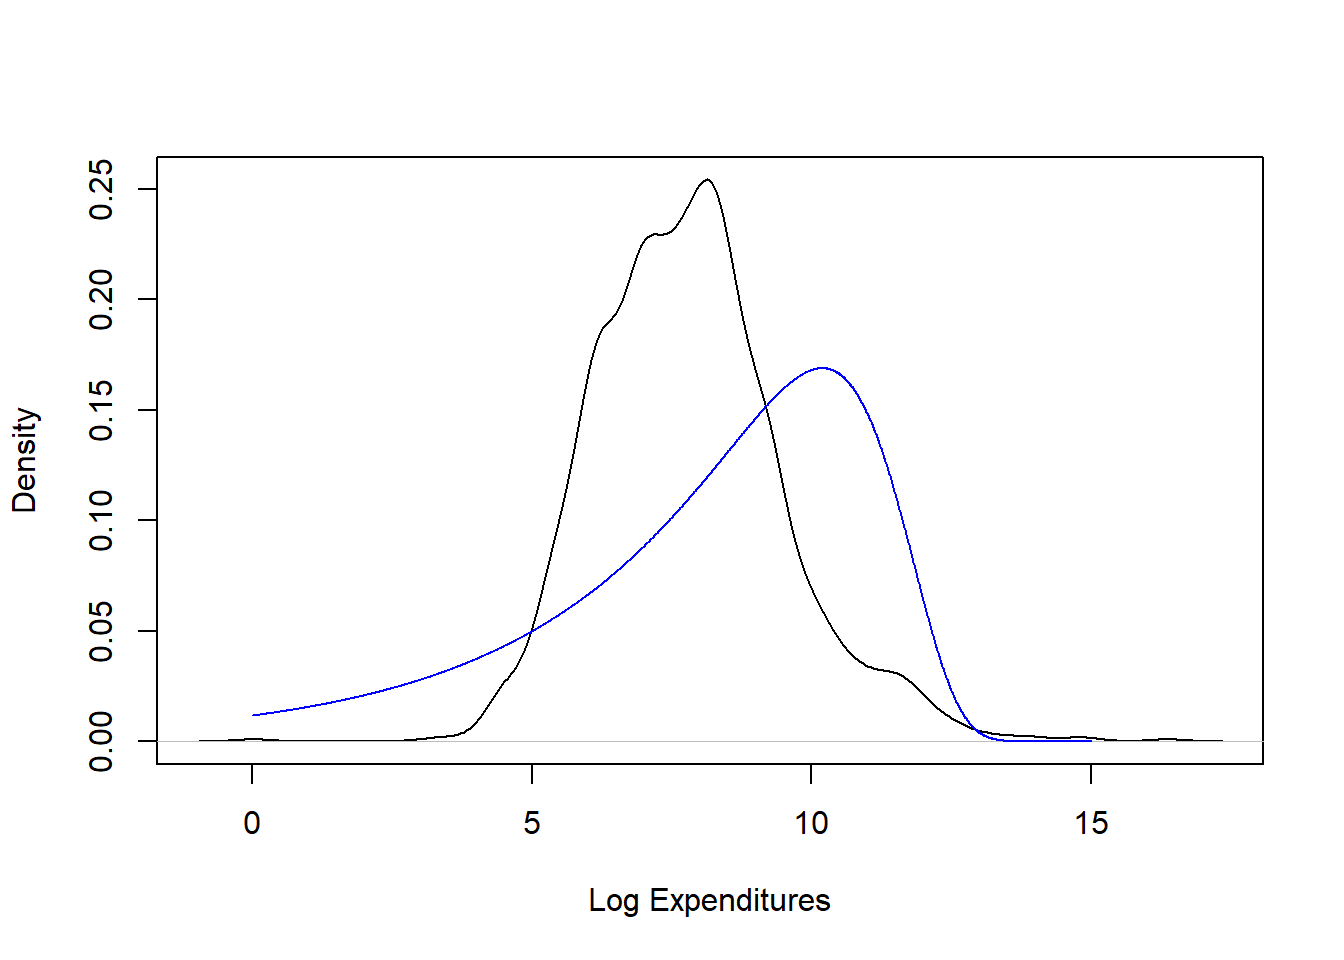
\includegraphics{R_for_Loss_Data_Analytics_files/figure-latex/unnamed-chunk-55-1} \end{center}

\begin{Shaded}
\begin{Highlighting}[]
\KeywordTok{confint}\NormalTok{(fit.gamma, }\DataTypeTok{level =} \FloatTok{0.95}\NormalTok{)  }\CommentTok{# confidence intervals for model parameters }
\end{Highlighting}
\end{Shaded}

\begin{verbatim}
                  2.5 %    97.5 %
(Intercept):1 10.091533 10.287498
(Intercept):2 -1.294648 -1.176995
\end{verbatim}

\begin{Shaded}
\begin{Highlighting}[]
\KeywordTok{logLik}\NormalTok{(fit.gamma)                 }\CommentTok{# loglikelihood for gamma}
\end{Highlighting}
\end{Shaded}

\begin{verbatim}
[1] -14150.59
\end{verbatim}

\begin{Shaded}
\begin{Highlighting}[]
\KeywordTok{AIC}\NormalTok{(fit.gamma)                    }\CommentTok{# AIC for gamma}
\end{Highlighting}
\end{Shaded}

\begin{verbatim}
[1] 28305.17
\end{verbatim}

\begin{Shaded}
\begin{Highlighting}[]
\KeywordTok{BIC}\NormalTok{(fit.gamma)                    }\CommentTok{# BIC for gamma}
\end{Highlighting}
\end{Shaded}

\begin{verbatim}
[1] 28315.63
\end{verbatim}

\begin{Shaded}
\begin{Highlighting}[]
\KeywordTok{vcov}\NormalTok{(fit.gamma)                   }\CommentTok{# covariance matrix for model parameters }
\end{Highlighting}
\end{Shaded}

\begin{verbatim}
              (Intercept):1 (Intercept):2
(Intercept):1   0.002499196  0.0000000000
(Intercept):2   0.000000000  0.0009008397
\end{verbatim}

\begin{Shaded}
\begin{Highlighting}[]
\CommentTok{# Here is a check on the formulas}
\CommentTok{# AIC using formula : -2 * (loglik) + 2 * (number of parameters)}
\OperatorTok{-}\DecValTok{2} \OperatorTok{*}\StringTok{ }\NormalTok{(}\KeywordTok{logLik}\NormalTok{(fit.gamma)) }\OperatorTok{+}\StringTok{ }\DecValTok{2} \OperatorTok{*}\StringTok{ }\NormalTok{(}\KeywordTok{length}\NormalTok{(}\KeywordTok{coef}\NormalTok{(fit.gamma)))}
\end{Highlighting}
\end{Shaded}

\begin{verbatim}
[1] 28305.17
\end{verbatim}

\begin{Shaded}
\begin{Highlighting}[]
\CommentTok{# BIC using formula : -2 * (loglik) + (number of parameters) * (log(n))}
\OperatorTok{-}\DecValTok{2} \OperatorTok{*}\StringTok{ }\NormalTok{(}\KeywordTok{logLik}\NormalTok{(fit.gamma)) }\OperatorTok{+}\StringTok{ }\KeywordTok{length}\NormalTok{(}\KeywordTok{coef}\NormalTok{(fit.gamma, }\DataTypeTok{matrix =} \OtherTok{TRUE}\NormalTok{)) }\OperatorTok{*}\StringTok{ }\KeywordTok{log}\NormalTok{(}\KeywordTok{nrow}\NormalTok{(claim_data))}
\end{Highlighting}
\end{Shaded}

\begin{verbatim}
[1] 28315.63
\end{verbatim}

\begin{Shaded}
\begin{Highlighting}[]
\CommentTok{# Alternatively, we could a gamma distribution using glm}
\KeywordTok{library}\NormalTok{(MASS)}
\NormalTok{fit.gamma_}\DecValTok{2}\NormalTok{ <-}\StringTok{ }\KeywordTok{glm}\NormalTok{(Claim }\OperatorTok{~}\StringTok{ }\DecValTok{1}\NormalTok{, }\DataTypeTok{data =}\NormalTok{ claim_data, }\DataTypeTok{family =} \KeywordTok{Gamma}\NormalTok{(}\DataTypeTok{link =}\NormalTok{ log)) }
\KeywordTok{summary}\NormalTok{(fit.gamma_}\DecValTok{2}\NormalTok{, }\DataTypeTok{dispersion =} \KeywordTok{gamma.dispersion}\NormalTok{(fit.gamma_}\DecValTok{2}\NormalTok{)) }
\end{Highlighting}
\end{Shaded}

\begin{verbatim}

Call:
glm(formula = Claim ~ 1, family = Gamma(link = log), data = claim_data)

Deviance Residuals: 
   Min      1Q  Median      3Q     Max  
-4.287  -2.258  -1.764  -1.178  30.926  

Coefficients:
            Estimate Std. Error z value Pr(>|z|)    
(Intercept) 10.18952    0.04999   203.8   <2e-16 ***
---
Signif. codes:  0 '***' 0.001 '**' 0.01 '*' 0.05 '.' 0.1 ' ' 1

(Dispersion parameter for Gamma family taken to be 3.441204)

    Null deviance: 6569.1  on 1376  degrees of freedom
Residual deviance: 6569.1  on 1376  degrees of freedom
AIC: 28414

Number of Fisher Scoring iterations: 14
\end{verbatim}

\begin{Shaded}
\begin{Highlighting}[]
\NormalTok{( theta <-}\StringTok{ }\KeywordTok{exp}\NormalTok{(}\KeywordTok{coef}\NormalTok{(fit.gamma_}\DecValTok{2}\NormalTok{)) }\OperatorTok{*}\StringTok{ }\KeywordTok{gamma.dispersion}\NormalTok{(fit.gamma_}\DecValTok{2}\NormalTok{) )  }\CommentTok{#theta = mu / alpha}
\end{Highlighting}
\end{Shaded}

\begin{verbatim}
(Intercept) 
   91613.78 
\end{verbatim}

\begin{Shaded}
\begin{Highlighting}[]
\NormalTok{( alpha <-}\StringTok{ }\DecValTok{1} \OperatorTok{/}\StringTok{ }\KeywordTok{gamma.dispersion}\NormalTok{(fit.gamma_}\DecValTok{2}\NormalTok{) )}
\end{Highlighting}
\end{Shaded}

\begin{verbatim}
[1] 0.2905959
\end{verbatim}

\begin{Shaded}
\begin{Highlighting}[]
\KeywordTok{logLik}\NormalTok{(fit.gamma_}\DecValTok{2}\NormalTok{)  }\CommentTok{# log - likelihood slightly different from vglm}
\end{Highlighting}
\end{Shaded}

\begin{verbatim}
'log Lik.' -14204.77 (df=2)
\end{verbatim}

\begin{Shaded}
\begin{Highlighting}[]
\KeywordTok{AIC}\NormalTok{(fit.gamma_}\DecValTok{2}\NormalTok{)     }\CommentTok{# AIC}
\end{Highlighting}
\end{Shaded}

\begin{verbatim}
[1] 28413.53
\end{verbatim}

\begin{Shaded}
\begin{Highlighting}[]
\KeywordTok{BIC}\NormalTok{(fit.gamma_}\DecValTok{2}\NormalTok{)     }\CommentTok{# BIC}
\end{Highlighting}
\end{Shaded}

\begin{verbatim}
[1] 28423.99
\end{verbatim}

Note : The output from \texttt{coef(fit.gamma)} uses the
parameterization \(\mu = \theta * \alpha\).
\texttt{coef(fit.gamma){[}1{]}} = \(\log(\mu)\) and
\texttt{coef(fit.gamma){[}2{]}} = \(\log(\alpha)\), which implies ,
\(\alpha\) = \texttt{exp(coef(fit.gamma){[}2{]})} and
\(\theta = \mu / \alpha\) =
\texttt{exp(coef(fit.gamma){[}1{]})\ /\ exp(coef(fit.gamma){[}2{]})}.

\subsection{Inference Assuming a Pareto
Distribution}\label{inference-assuming-a-pareto-distribution}

The results below assume that the data follow a Pareto distribution and
uses\texttt{VGAM} library for estimation of parameters.

\begin{Shaded}
\begin{Highlighting}[]
\NormalTok{fit.pareto <-}\StringTok{ }\KeywordTok{vglm}\NormalTok{(Claim }\OperatorTok{~}\StringTok{ }\DecValTok{1}\NormalTok{, paretoII, }\DataTypeTok{loc =} \DecValTok{0}\NormalTok{, }\DataTypeTok{data =}\NormalTok{ claim_data)}
\KeywordTok{summary}\NormalTok{(fit.pareto)}
\end{Highlighting}
\end{Shaded}

\begin{verbatim}

Call:
vglm(formula = Claim ~ 1, family = paretoII, data = claim_data, 
    loc = 0)


Pearson residuals:
                Min      1Q Median     3Q   Max
loge(scale)  -6.332 -0.8289 0.1875 0.8832 1.174
loge(shape) -10.638  0.0946 0.4047 0.4842 0.513

Coefficients: 
                Estimate Std. Error z value Pr(>|z|)    
(Intercept):1  7.7329210  0.0933332  82.853   <2e-16 ***
(Intercept):2 -0.0008753  0.0538642  -0.016    0.987    
---
Signif. codes:  0 '***' 0.001 '**' 0.01 '*' 0.05 '.' 0.1 ' ' 1

Number of linear predictors:  2 

Names of linear predictors: loge(scale), loge(shape)

Log-likelihood: -13404.64 on 2752 degrees of freedom

Number of iterations: 5 

No Hauck-Donner effect found in any of the estimates
\end{verbatim}

\begin{Shaded}
\begin{Highlighting}[]
\KeywordTok{head}\NormalTok{(}\KeywordTok{fitted}\NormalTok{(fit.pareto))}
\end{Highlighting}
\end{Shaded}

\begin{verbatim}
        [,1]
[1,] 2285.03
[2,] 2285.03
[3,] 2285.03
[4,] 2285.03
[5,] 2285.03
[6,] 2285.03
\end{verbatim}

\begin{Shaded}
\begin{Highlighting}[]
\KeywordTok{coef}\NormalTok{(fit.pareto)}
\end{Highlighting}
\end{Shaded}

\begin{verbatim}
(Intercept):1 (Intercept):2 
 7.7329210483 -0.0008752515 
\end{verbatim}

\begin{Shaded}
\begin{Highlighting}[]
\KeywordTok{exp}\NormalTok{(}\KeywordTok{coef}\NormalTok{(fit.pareto))}
\end{Highlighting}
\end{Shaded}

\begin{verbatim}
(Intercept):1 (Intercept):2 
 2282.2590626     0.9991251 
\end{verbatim}

\begin{Shaded}
\begin{Highlighting}[]
\KeywordTok{confint}\NormalTok{(fit.pareto, }\DataTypeTok{level =} \FloatTok{0.95}\NormalTok{)  }\CommentTok{# confidence intervals for model parameters }
\end{Highlighting}
\end{Shaded}

\begin{verbatim}
                   2.5 %    97.5 %
(Intercept):1  7.5499914 7.9158507
(Intercept):2 -0.1064471 0.1046966
\end{verbatim}

\begin{Shaded}
\begin{Highlighting}[]
\KeywordTok{logLik}\NormalTok{(fit.pareto)                 }\CommentTok{# loglikelihood for Pareto}
\end{Highlighting}
\end{Shaded}

\begin{verbatim}
[1] -13404.64
\end{verbatim}

\begin{Shaded}
\begin{Highlighting}[]
\KeywordTok{AIC}\NormalTok{(fit.pareto)                    }\CommentTok{# AIC for Pareto}
\end{Highlighting}
\end{Shaded}

\begin{verbatim}
[1] 26813.29
\end{verbatim}

\begin{Shaded}
\begin{Highlighting}[]
\KeywordTok{BIC}\NormalTok{(fit.pareto)                    }\CommentTok{# BIC for Pareto}
\end{Highlighting}
\end{Shaded}

\begin{verbatim}
[1] 26823.74
\end{verbatim}

\begin{Shaded}
\begin{Highlighting}[]
\KeywordTok{vcov}\NormalTok{(fit.pareto)                   }\CommentTok{# covariance matrix for model parameters }
\end{Highlighting}
\end{Shaded}

\begin{verbatim}
              (Intercept):1 (Intercept):2
(Intercept):1   0.008711083   0.004352904
(Intercept):2   0.004352904   0.002901350
\end{verbatim}

\subsection{Inference Assuming an Exponential
Distribution}\label{inference-assuming-an-exponential-distribution}

The results below assume that the data follow an exponential
distribution and uses\texttt{VGAM} library for estimation of parameters.

\begin{Shaded}
\begin{Highlighting}[]
\NormalTok{fit.exp <-}\StringTok{ }\KeywordTok{vglm}\NormalTok{(Claim }\OperatorTok{~}\StringTok{ }\DecValTok{1}\NormalTok{, exponential, }\DataTypeTok{data =}\NormalTok{ claim_data)}
\KeywordTok{summary}\NormalTok{(fit.exp)}
\end{Highlighting}
\end{Shaded}

\begin{verbatim}

Call:
vglm(formula = Claim ~ 1, family = exponential, data = claim_data)


Pearson residuals:
              Min     1Q Median     3Q Max
loge(rate) -484.4 0.7682 0.9155 0.9704   1

Coefficients: 
             Estimate Std. Error z value Pr(>|z|)    
(Intercept) -10.18952    0.02695  -378.1   <2e-16 ***
---
Signif. codes:  0 '***' 0.001 '**' 0.01 '*' 0.05 '.' 0.1 ' ' 1

Number of linear predictors:  1 

Name of linear predictor: loge(rate) 

Residual deviance: 6569.099 on 1376 degrees of freedom

Log-likelihood: -15407.96 on 1376 degrees of freedom

Number of iterations: 6 

No Hauck-Donner effect found in any of the estimates
\end{verbatim}

\begin{Shaded}
\begin{Highlighting}[]
\NormalTok{( }\DataTypeTok{theta =} \DecValTok{1} \OperatorTok{/}\StringTok{ }\KeywordTok{exp}\NormalTok{(}\KeywordTok{coef}\NormalTok{(fit.exp)) )}
\end{Highlighting}
\end{Shaded}

\begin{verbatim}
(Intercept) 
   26622.59 
\end{verbatim}

\begin{Shaded}
\begin{Highlighting}[]
\CommentTok{# Can also fit using the "glm" package}
\NormalTok{fit.exp2 <-}\StringTok{ }\KeywordTok{glm}\NormalTok{(Claim }\OperatorTok{~}\StringTok{ }\DecValTok{1}\NormalTok{, }\DataTypeTok{data =}\NormalTok{ claim_data, }\DataTypeTok{family =} \KeywordTok{Gamma}\NormalTok{(}\DataTypeTok{link =}\NormalTok{ log)) }
\KeywordTok{summary}\NormalTok{(fit.exp2, }\DataTypeTok{dispersion =} \DecValTok{1}\NormalTok{)}
\end{Highlighting}
\end{Shaded}

\begin{verbatim}

Call:
glm(formula = Claim ~ 1, family = Gamma(link = log), data = claim_data)

Deviance Residuals: 
   Min      1Q  Median      3Q     Max  
-4.287  -2.258  -1.764  -1.178  30.926  

Coefficients:
            Estimate Std. Error z value Pr(>|z|)    
(Intercept) 10.18952    0.02695   378.1   <2e-16 ***
---
Signif. codes:  0 '***' 0.001 '**' 0.01 '*' 0.05 '.' 0.1 ' ' 1

(Dispersion parameter for Gamma family taken to be 1)

    Null deviance: 6569.1  on 1376  degrees of freedom
Residual deviance: 6569.1  on 1376  degrees of freedom
AIC: 28414

Number of Fisher Scoring iterations: 14
\end{verbatim}

\begin{Shaded}
\begin{Highlighting}[]
\NormalTok{( theta <-}\StringTok{ }\KeywordTok{exp}\NormalTok{(}\KeywordTok{coef}\NormalTok{(fit.exp2)) )  }
\end{Highlighting}
\end{Shaded}

\begin{verbatim}
(Intercept) 
   26622.59 
\end{verbatim}

\subsection{Inference Assuming a Generalized Beta Distribution of the
Second Kind (GB2)
Distribution}\label{inference-assuming-a-generalized-beta-distribution-of-the-second-kind-gb2-distribution}

The results below assume that the data follow a GB2 distribution and
uses the maximum likelihood technique for parameter estimation.

\begin{Shaded}
\begin{Highlighting}[]
\CommentTok{# Inference assuming a GB2 Distribution - this is more complicated}
\CommentTok{# The likelihood functon of GB2 distribution (negative for optimization)}
\NormalTok{lik_gb2 <-}\StringTok{ }\ControlFlowTok{function}\NormalTok{ (param) \{}
\NormalTok{  a_}\DecValTok{1}\NormalTok{ <-}\StringTok{ }\NormalTok{param[}\DecValTok{1}\NormalTok{]}
\NormalTok{  a_}\DecValTok{2}\NormalTok{ <-}\StringTok{ }\NormalTok{param[}\DecValTok{2}\NormalTok{]}
\NormalTok{  mu <-}\StringTok{ }\NormalTok{param[}\DecValTok{3}\NormalTok{]}
\NormalTok{  sigma <-}\StringTok{ }\NormalTok{param[}\DecValTok{4}\NormalTok{]}
\NormalTok{  yt <-}\StringTok{ }\NormalTok{(}\KeywordTok{log}\NormalTok{(claim_data}\OperatorTok{$}\NormalTok{Claim) }\OperatorTok{-}\StringTok{ }\NormalTok{mu) }\OperatorTok{/}\StringTok{ }\NormalTok{sigma}
\NormalTok{  logexpyt <-}\StringTok{ }\KeywordTok{ifelse}\NormalTok{(yt }\OperatorTok{>}\StringTok{ }\DecValTok{23}\NormalTok{, yt, }\KeywordTok{log}\NormalTok{(}\DecValTok{1} \OperatorTok{+}\StringTok{ }\KeywordTok{exp}\NormalTok{(yt)))}
\NormalTok{  logdens <-}\StringTok{ }\NormalTok{a_}\DecValTok{1} \OperatorTok{*}\StringTok{ }\NormalTok{yt }\OperatorTok{-}\StringTok{ }\KeywordTok{log}\NormalTok{(sigma) }\OperatorTok{-}\StringTok{ }\KeywordTok{log}\NormalTok{(}\KeywordTok{beta}\NormalTok{(a_}\DecValTok{1}\NormalTok{,a_}\DecValTok{2}\NormalTok{)) }\OperatorTok{-}\StringTok{ }
\StringTok{    }\NormalTok{(a_}\DecValTok{1}\OperatorTok{+}\NormalTok{a_}\DecValTok{2}\NormalTok{) }\OperatorTok{*}\StringTok{ }\NormalTok{logexpyt }\OperatorTok{-}\StringTok{ }\KeywordTok{log}\NormalTok{(claim_data}\OperatorTok{$}\NormalTok{Claim) }
  \KeywordTok{return}\NormalTok{(}\OperatorTok{-}\KeywordTok{sum}\NormalTok{(logdens))}
\NormalTok{\}}
\CommentTok{# "optim" is a general purpose minimization function}
\NormalTok{gb2_bop <-}\StringTok{ }\KeywordTok{optim}\NormalTok{(}\KeywordTok{c}\NormalTok{(}\DecValTok{1}\NormalTok{, }\DecValTok{1}\NormalTok{, }\DecValTok{0}\NormalTok{, }\DecValTok{1}\NormalTok{), lik_gb2, }\DataTypeTok{method =} \KeywordTok{c}\NormalTok{(}\StringTok{"L-BFGS-B"}\NormalTok{), }
                 \DataTypeTok{lower =} \KeywordTok{c}\NormalTok{(}\FloatTok{0.01}\NormalTok{, }\FloatTok{0.01}\NormalTok{, }\OperatorTok{-}\DecValTok{500}\NormalTok{, }\FloatTok{0.01}\NormalTok{), }
                 \DataTypeTok{upper =} \KeywordTok{c}\NormalTok{(}\DecValTok{500}\NormalTok{, }\DecValTok{500}\NormalTok{, }\DecValTok{500}\NormalTok{, }\DecValTok{500}\NormalTok{), }\DataTypeTok{hessian =} \OtherTok{TRUE}\NormalTok{)}

\CommentTok{# Estimates}
\NormalTok{gb2_bop}\OperatorTok{$}\NormalTok{par}
\end{Highlighting}
\end{Shaded}

\begin{verbatim}
[1] 2.830928 1.202500 6.328981 1.294552
\end{verbatim}

\begin{Shaded}
\begin{Highlighting}[]
\CommentTok{# Standard error}
\KeywordTok{sqrt}\NormalTok{(}\KeywordTok{diag}\NormalTok{(}\KeywordTok{solve}\NormalTok{(gb2_bop}\OperatorTok{$}\NormalTok{hessian)))}
\end{Highlighting}
\end{Shaded}

\begin{verbatim}
[1] 0.9997743 0.2918469 0.3901929 0.2190362
\end{verbatim}

\begin{Shaded}
\begin{Highlighting}[]
\CommentTok{# t-statistics}
\NormalTok{( tstat <-}\StringTok{ }\NormalTok{gb2_bop}\OperatorTok{$}\NormalTok{par }\OperatorTok{/}\StringTok{ }\KeywordTok{sqrt}\NormalTok{(}\KeywordTok{diag}\NormalTok{(}\KeywordTok{solve}\NormalTok{(gb2_bop}\OperatorTok{$}\NormalTok{hessian))) )}
\end{Highlighting}
\end{Shaded}

\begin{verbatim}
[1]  2.831567  4.120313 16.220133  5.910217
\end{verbatim}

\begin{Shaded}
\begin{Highlighting}[]
\CommentTok{# density for GB II}
\NormalTok{gb2_density <-}\StringTok{ }\ControlFlowTok{function}\NormalTok{(x)\{}
\NormalTok{  a_}\DecValTok{1}\NormalTok{ <-}\StringTok{ }\NormalTok{gb2_bop}\OperatorTok{$}\NormalTok{par[}\DecValTok{1}\NormalTok{]}
\NormalTok{  a_}\DecValTok{2}\NormalTok{ <-}\StringTok{ }\NormalTok{gb2_bop}\OperatorTok{$}\NormalTok{par[}\DecValTok{2}\NormalTok{]}
\NormalTok{  mu <-}\StringTok{ }\NormalTok{gb2_bop}\OperatorTok{$}\NormalTok{par[}\DecValTok{3}\NormalTok{]}
\NormalTok{  sigma <-}\StringTok{ }\NormalTok{gb2_bop}\OperatorTok{$}\NormalTok{par[}\DecValTok{4}\NormalTok{]}
\NormalTok{  xt <-}\StringTok{ }\NormalTok{(}\KeywordTok{log}\NormalTok{(x) }\OperatorTok{-}\StringTok{ }\NormalTok{mu) }\OperatorTok{/}\StringTok{ }\NormalTok{sigma}
\NormalTok{  logexpxt<-}\KeywordTok{ifelse}\NormalTok{ (xt }\OperatorTok{>}\StringTok{ }\DecValTok{23}\NormalTok{, yt, }\KeywordTok{log}\NormalTok{(}\DecValTok{1} \OperatorTok{+}\StringTok{ }\KeywordTok{exp}\NormalTok{(xt)))}
\NormalTok{  logdens <-}\StringTok{ }\NormalTok{a_}\DecValTok{1} \OperatorTok{*}\StringTok{ }\NormalTok{xt }\OperatorTok{-}\StringTok{ }\KeywordTok{log}\NormalTok{(sigma) }\OperatorTok{-}\StringTok{ }\KeywordTok{log}\NormalTok{(}\KeywordTok{beta}\NormalTok{(a_}\DecValTok{1}\NormalTok{, a_}\DecValTok{2}\NormalTok{)) }\OperatorTok{-}\StringTok{ }
\StringTok{    }\NormalTok{(a_}\DecValTok{1}\OperatorTok{+}\NormalTok{a_}\DecValTok{2}\NormalTok{) }\OperatorTok{*}\StringTok{ }\NormalTok{logexpxt }\OperatorTok{-}\StringTok{ }\KeywordTok{log}\NormalTok{(x) }
  \KeywordTok{exp}\NormalTok{(logdens)}
\NormalTok{\}}

\CommentTok{# AIC using formula : -2 * (loglik) + 2 * (number of parameters)}
\OperatorTok{-}\DecValTok{2} \OperatorTok{*}\StringTok{ }\NormalTok{( }\KeywordTok{sum}\NormalTok{(}\KeywordTok{log}\NormalTok{(}\KeywordTok{gb2_density}\NormalTok{(claim_data}\OperatorTok{$}\NormalTok{Claim))) ) }\OperatorTok{+}\StringTok{ }\DecValTok{2} \OperatorTok{*}\StringTok{ }\DecValTok{4}
\end{Highlighting}
\end{Shaded}

\begin{verbatim}
[1] 26768.13
\end{verbatim}

\begin{Shaded}
\begin{Highlighting}[]
\CommentTok{# BIC using formula : -2 * (loglik) + (number of parameters) * (log(n))}
\OperatorTok{-}\DecValTok{2} \OperatorTok{*}\NormalTok{( }\KeywordTok{sum}\NormalTok{(}\KeywordTok{log}\NormalTok{(}\KeywordTok{gb2_density}\NormalTok{(claim_data}\OperatorTok{$}\NormalTok{Claim))) ) }\OperatorTok{+}\StringTok{ }\DecValTok{4} \OperatorTok{*}\StringTok{ }\KeywordTok{log}\NormalTok{(}\KeywordTok{nrow}\NormalTok{(claim_data))}
\end{Highlighting}
\end{Shaded}

\begin{verbatim}
[1] 26789.04
\end{verbatim}

\section{Plotting the Fit Using Densities (on a Logarithmic
Scale)}\label{plotting-the-fit-using-densities-on-a-logarithmic-scale}

This section plots on a logarithmic scale, the smooth (nonparametric)
density of claims and overlays the densities of the distributions
considered above.

\begin{Shaded}
\begin{Highlighting}[]
\CommentTok{# None of these distributions is doing a great job....}
\KeywordTok{plot}\NormalTok{(}\KeywordTok{density}\NormalTok{(}\KeywordTok{log}\NormalTok{(claim_data}\OperatorTok{$}\NormalTok{Claim)), }\DataTypeTok{main =} \StringTok{""}\NormalTok{, }\DataTypeTok{xlab =} \StringTok{"Log Expenditures"}\NormalTok{,}
     \DataTypeTok{ylim =} \KeywordTok{c}\NormalTok{(}\DecValTok{0}\NormalTok{ ,}\FloatTok{0.37}\NormalTok{))}
\NormalTok{x <-}\StringTok{ }\KeywordTok{seq}\NormalTok{(}\DecValTok{0}\NormalTok{, }\DecValTok{15}\NormalTok{, }\DataTypeTok{by =} \FloatTok{0.01}\NormalTok{)}
\NormalTok{fexp_ex <-}\StringTok{ }\KeywordTok{dgamma}\NormalTok{(}\KeywordTok{exp}\NormalTok{(x), }\DataTypeTok{scale =} \KeywordTok{exp}\NormalTok{(}\OperatorTok{-}\KeywordTok{coef}\NormalTok{(fit.exp)), }\DataTypeTok{shape =} \DecValTok{1}\NormalTok{) }\OperatorTok{*}\StringTok{ }\KeywordTok{exp}\NormalTok{(x)}
\KeywordTok{lines}\NormalTok{(x, fexp_ex, }\DataTypeTok{col =} \StringTok{"red"}\NormalTok{)}
\NormalTok{fgamma_ex <-}\StringTok{ }\KeywordTok{dgamma}\NormalTok{(}\KeywordTok{exp}\NormalTok{(x), }\DataTypeTok{shape =}\NormalTok{ alpha, }\DataTypeTok{scale =}\NormalTok{ theta) }\OperatorTok{*}\StringTok{ }\KeywordTok{exp}\NormalTok{(x)}
\KeywordTok{lines}\NormalTok{(x, fgamma_ex, }\DataTypeTok{col =} \StringTok{"blue"}\NormalTok{)}
\NormalTok{fpareto_ex <-}\StringTok{ }\KeywordTok{dparetoII}\NormalTok{(}\KeywordTok{exp}\NormalTok{(x), }\DataTypeTok{loc =} \DecValTok{0}\NormalTok{, }\DataTypeTok{shape =} \KeywordTok{exp}\NormalTok{(}\KeywordTok{coef}\NormalTok{(fit.pareto)[}\DecValTok{2}\NormalTok{]), }
                        \DataTypeTok{scale =} \KeywordTok{exp}\NormalTok{(}\KeywordTok{coef}\NormalTok{(fit.pareto)[}\DecValTok{1}\NormalTok{])) }\OperatorTok{*}\StringTok{ }\KeywordTok{exp}\NormalTok{(x)}
\KeywordTok{lines}\NormalTok{(x, fpareto_ex, }\DataTypeTok{col =} \StringTok{"purple"}\NormalTok{)}
\NormalTok{flnorm_ex <-}\StringTok{ }\KeywordTok{dlnorm}\NormalTok{(}\KeywordTok{exp}\NormalTok{(x), }\DataTypeTok{mean =} \KeywordTok{coef}\NormalTok{(fit.LN)[}\DecValTok{1}\NormalTok{],}
                    \DataTypeTok{sd =} \KeywordTok{exp}\NormalTok{(}\KeywordTok{coef}\NormalTok{(fit.LN)[}\DecValTok{2}\NormalTok{])) }\OperatorTok{*}\StringTok{ }\KeywordTok{exp}\NormalTok{(x)}
\KeywordTok{lines}\NormalTok{(x, flnorm_ex, }\DataTypeTok{col =} \StringTok{"lightblue"}\NormalTok{)}
\CommentTok{# Density for GB II}
\NormalTok{gb2_density <-}\StringTok{ }\ControlFlowTok{function}\NormalTok{ (x) \{}
\NormalTok{  a_}\DecValTok{1}\NormalTok{ <-}\StringTok{ }\NormalTok{gb2_bop}\OperatorTok{$}\NormalTok{par[}\DecValTok{1}\NormalTok{]}
\NormalTok{  a_}\DecValTok{2}\NormalTok{ <-}\StringTok{ }\NormalTok{gb2_bop}\OperatorTok{$}\NormalTok{par[}\DecValTok{2}\NormalTok{]}
\NormalTok{  mu <-}\StringTok{ }\NormalTok{gb2_bop}\OperatorTok{$}\NormalTok{par[}\DecValTok{3}\NormalTok{]}
\NormalTok{  sigma <-}\StringTok{ }\NormalTok{gb2_bop}\OperatorTok{$}\NormalTok{par[}\DecValTok{4}\NormalTok{]}
\NormalTok{  xt <-}\StringTok{ }\NormalTok{(}\KeywordTok{log}\NormalTok{(x) }\OperatorTok{-}\StringTok{ }\NormalTok{mu) }\OperatorTok{/}\StringTok{ }\NormalTok{sigma}
\NormalTok{  logexpxt <-}\StringTok{ }\KeywordTok{ifelse}\NormalTok{ (xt }\OperatorTok{>}\StringTok{ }\DecValTok{23}\NormalTok{, yt, }\KeywordTok{log}\NormalTok{(}\DecValTok{1} \OperatorTok{+}\StringTok{ }\KeywordTok{exp}\NormalTok{(xt)))}
\NormalTok{  logdens <-}\StringTok{ }\NormalTok{a_}\DecValTok{1} \OperatorTok{*}\StringTok{ }\NormalTok{xt }\OperatorTok{-}\StringTok{ }\KeywordTok{log}\NormalTok{(sigma) }\OperatorTok{-}\StringTok{ }\KeywordTok{log}\NormalTok{(}\KeywordTok{beta}\NormalTok{(a_}\DecValTok{1}\NormalTok{, a_}\DecValTok{2}\NormalTok{)) }\OperatorTok{-}\StringTok{ }
\StringTok{    }\NormalTok{(a_}\DecValTok{1}\OperatorTok{+}\NormalTok{a_}\DecValTok{2}\NormalTok{) }\OperatorTok{*}\StringTok{ }\NormalTok{logexpxt }\OperatorTok{-}\KeywordTok{log}\NormalTok{(x) }
  \KeywordTok{exp}\NormalTok{(logdens)}
\NormalTok{  \}}
\NormalTok{fGB2_ex =}\StringTok{ }\KeywordTok{gb2_density}\NormalTok{(}\KeywordTok{exp}\NormalTok{(x)) }\OperatorTok{*}\StringTok{ }\KeywordTok{exp}\NormalTok{(x)}
\KeywordTok{lines}\NormalTok{(x, fGB2_ex, }\DataTypeTok{col=}\StringTok{"green"}\NormalTok{)}

\KeywordTok{legend}\NormalTok{(}\StringTok{"topleft"}\NormalTok{, }\KeywordTok{c}\NormalTok{(}\StringTok{"log(claim_data$Claim)"}\NormalTok{, }\StringTok{"Exponential"}\NormalTok{, }\StringTok{"Gamma"}\NormalTok{, }\StringTok{"Pareto"}\NormalTok{, }
                    \StringTok{"lognormal"}\NormalTok{, }\StringTok{"GB2"}\NormalTok{), }
       \DataTypeTok{lty =} \DecValTok{1}\NormalTok{, }\DataTypeTok{col =} \KeywordTok{c}\NormalTok{(}\StringTok{"black"}\NormalTok{,}\StringTok{"red"}\NormalTok{,}\StringTok{"blue"}\NormalTok{,}\StringTok{"purple"}\NormalTok{,}\StringTok{"lightblue"}\NormalTok{,}\StringTok{"green"}\NormalTok{))}
\end{Highlighting}
\end{Shaded}

\begin{center}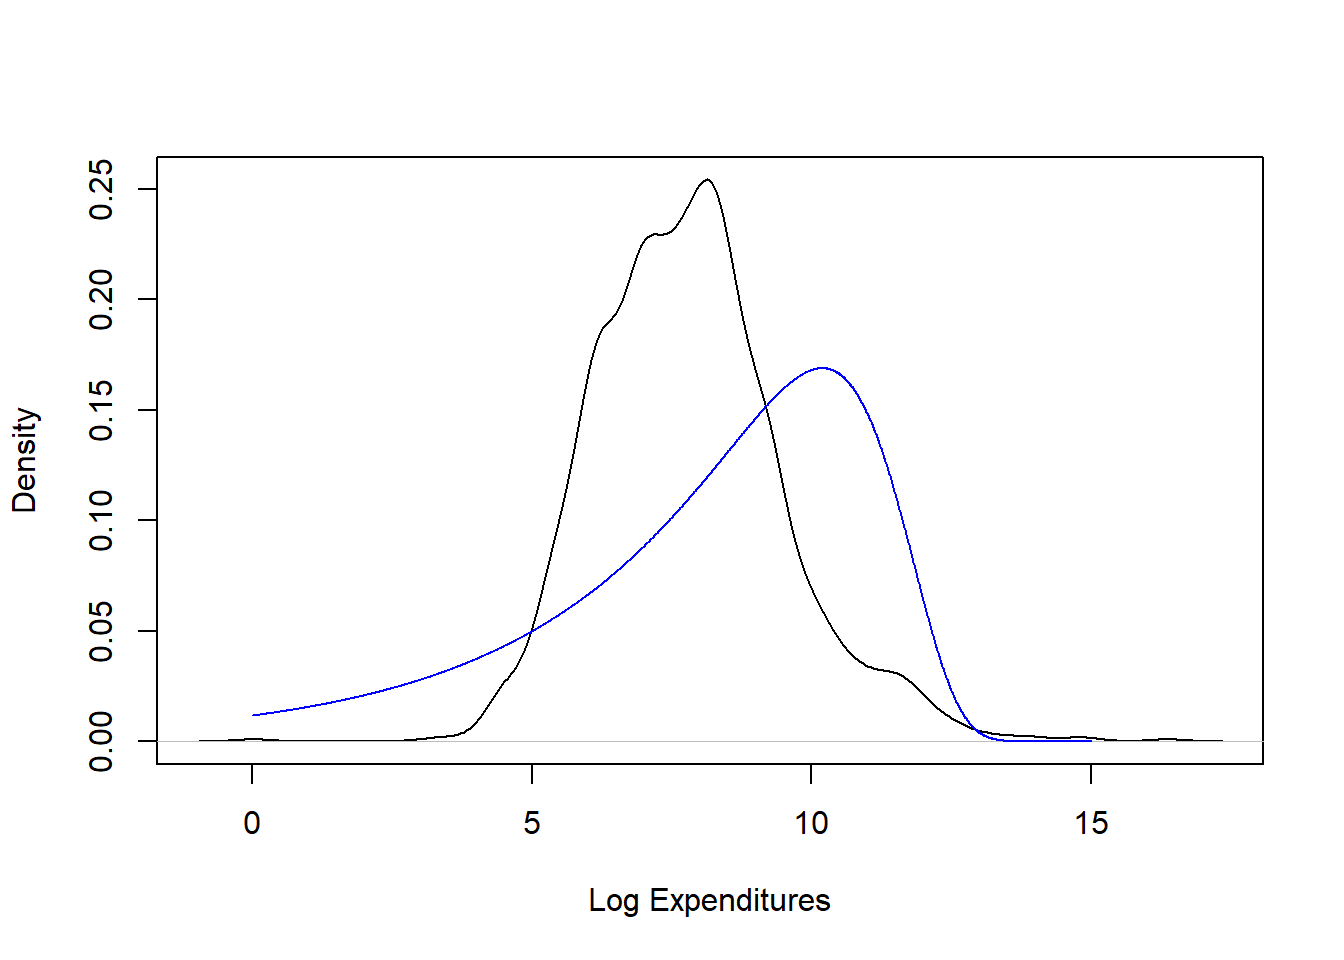
\includegraphics{R_for_Loss_Data_Analytics_files/figure-latex/unnamed-chunk-59-1} \end{center}

\section{Nonparametric Inference}\label{nonparametric-inference}

\subsection{Nonparametric Estimation
Tools}\label{nonparametric-estimation-tools}

This section illustrates non-parametric tools including moment
estimators, empirical distribution function, quantiles and density
estimators.

\subsubsection{Moment Estimators}\label{moment-estimators}

The \(kth\) moment \(EX^k\) is estimated by
\(\frac{1}{n}\sum_{i=1}^{n}X_i^k\). When \(k=1\) then the estimator is
called the sample mean. The central moment is defined as \(E(X-\mu)^k\).
When \(k=2\), then the central moment is called variance. Below
illustrates the mean and variance.

\begin{Shaded}
\begin{Highlighting}[]
\CommentTok{# Start with a simple example of ten points}
\NormalTok{( x_example <-}\StringTok{ }\KeywordTok{c}\NormalTok{(}\DecValTok{10}\NormalTok{, }\KeywordTok{rep}\NormalTok{(}\DecValTok{15}\NormalTok{,}\DecValTok{3}\NormalTok{), }\DecValTok{20}\NormalTok{, }\KeywordTok{rep}\NormalTok{(}\DecValTok{23}\NormalTok{,}\DecValTok{4}\NormalTok{), }\DecValTok{30}\NormalTok{) )}
\end{Highlighting}
\end{Shaded}

\begin{verbatim}
 [1] 10 15 15 15 20 23 23 23 23 30
\end{verbatim}

\begin{Shaded}
\begin{Highlighting}[]
\CommentTok{# Summary}
\KeywordTok{summary}\NormalTok{(x_example)  }\CommentTok{# mean }
\end{Highlighting}
\end{Shaded}

\begin{verbatim}
   Min. 1st Qu.  Median    Mean 3rd Qu.    Max. 
   10.0    15.0    21.5    19.7    23.0    30.0 
\end{verbatim}

\begin{Shaded}
\begin{Highlighting}[]
\KeywordTok{sd}\NormalTok{(x_example)}\OperatorTok{^}\DecValTok{2}  \CommentTok{# variance }
\end{Highlighting}
\end{Shaded}

\begin{verbatim}
[1] 34.45556
\end{verbatim}

\subsubsection{Empirical Distribution
Function}\label{empirical-distribution-function}

The graph below gives the empirical distribution function
\texttt{x\_example} dataset.

\begin{Shaded}
\begin{Highlighting}[]
\NormalTok{percentiles_x_example <-}\StringTok{ }\KeywordTok{ecdf}\NormalTok{(x_example)}

\CommentTok{# Empirical distribution function}
\KeywordTok{plot}\NormalTok{(percentiles_x_example, }\DataTypeTok{main =} \StringTok{""}\NormalTok{, }\DataTypeTok{xlab =} \StringTok{"x"}\NormalTok{)}
\end{Highlighting}
\end{Shaded}

\begin{center}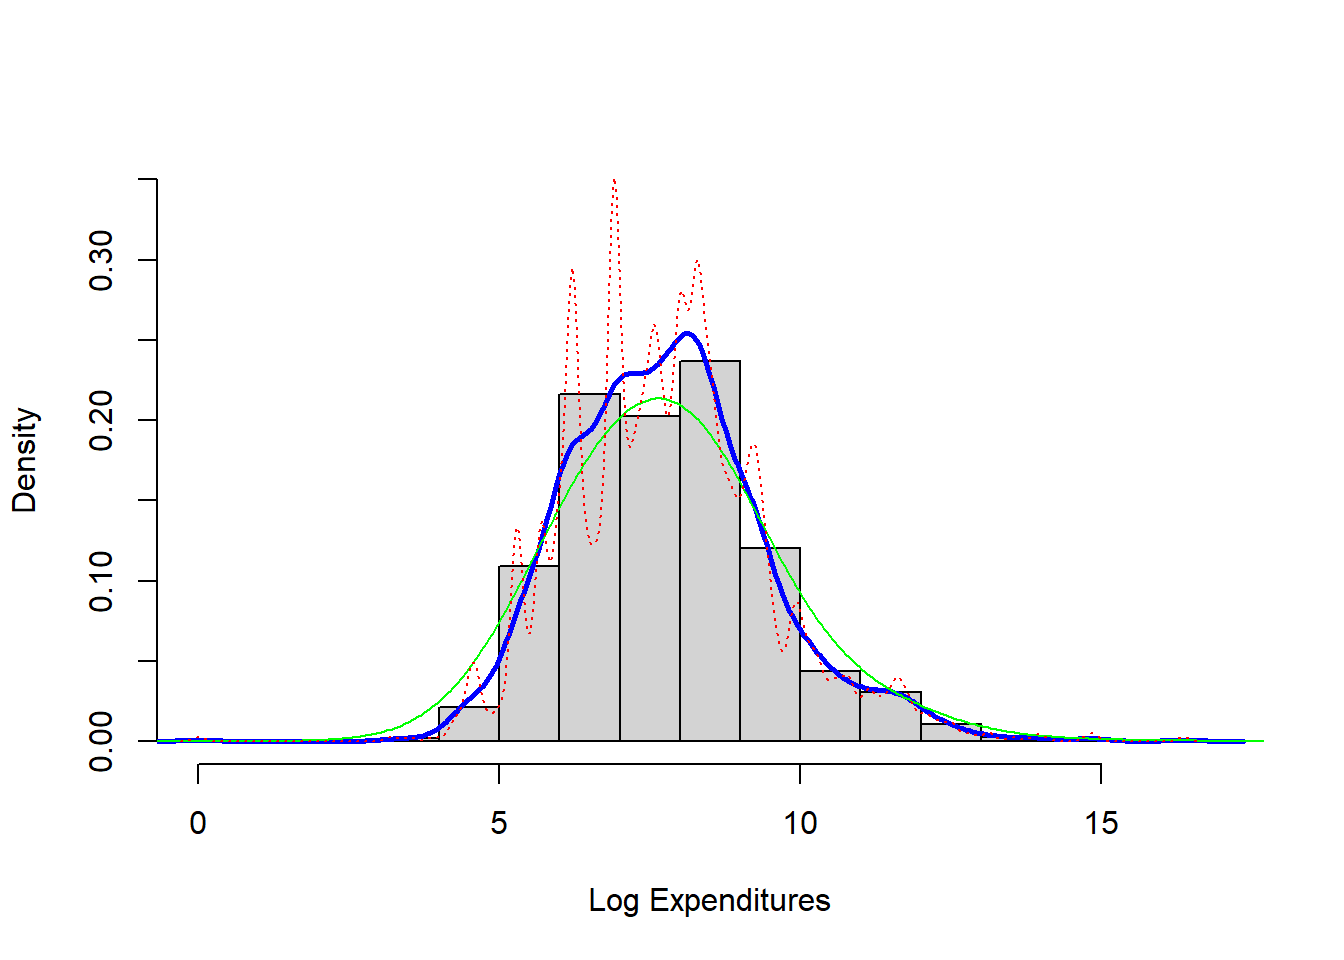
\includegraphics{R_for_Loss_Data_Analytics_files/figure-latex/unnamed-chunk-61-1} \end{center}

\subsubsection{Quantiles}\label{quantiles}

The results below gives the quantiles.

\begin{Shaded}
\begin{Highlighting}[]
\CommentTok{# Quantiles }
\KeywordTok{quantile}\NormalTok{(x_example)}
\end{Highlighting}
\end{Shaded}

\begin{verbatim}
  0%  25%  50%  75% 100% 
10.0 15.0 21.5 23.0 30.0 
\end{verbatim}

\begin{Shaded}
\begin{Highlighting}[]
\CommentTok{# Quantiles : set you own probabilities}
\KeywordTok{quantile}\NormalTok{(x_example, }\DataTypeTok{probs =} \KeywordTok{seq}\NormalTok{(}\DecValTok{0}\NormalTok{, }\DecValTok{1}\NormalTok{, }\FloatTok{0.333333}\NormalTok{))}
\end{Highlighting}
\end{Shaded}

\begin{verbatim}
      0% 33.3333% 66.6666% 99.9999% 
10.00000 15.00000 23.00000 29.99994 
\end{verbatim}

\begin{Shaded}
\begin{Highlighting}[]
\CommentTok{# help(quantile)}
\end{Highlighting}
\end{Shaded}

\subsubsection{Density Estimators}\label{density-estimators}

The results below gives the density plots using the uniform kernel and
triangular kernel.

\begin{Shaded}
\begin{Highlighting}[]
\CommentTok{# Density plot }
\KeywordTok{plot}\NormalTok{(}\KeywordTok{density}\NormalTok{(x_example), }\DataTypeTok{main =} \StringTok{""}\NormalTok{, }\DataTypeTok{xlab =} \StringTok{"x"}\NormalTok{)}
\end{Highlighting}
\end{Shaded}

\begin{center}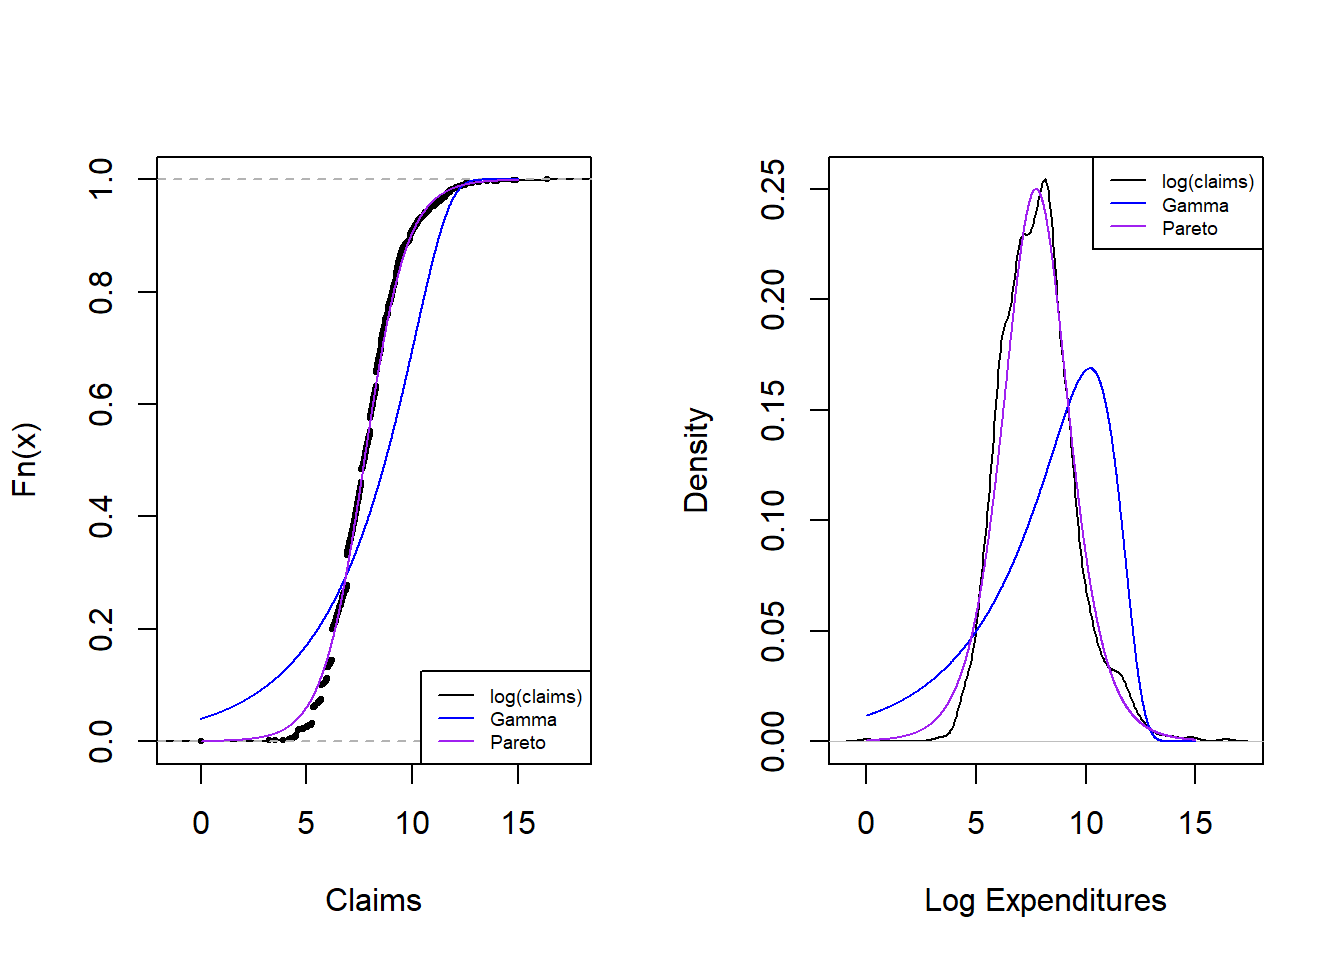
\includegraphics{R_for_Loss_Data_Analytics_files/figure-latex/unnamed-chunk-63-1} \end{center}

\begin{Shaded}
\begin{Highlighting}[]
\KeywordTok{plot}\NormalTok{(}\KeywordTok{density}\NormalTok{(x_example, }\DataTypeTok{bw =}\NormalTok{ .}\DecValTok{33}\NormalTok{), }\DataTypeTok{main =} \StringTok{""}\NormalTok{, }\DataTypeTok{xlab =} \StringTok{"x"}\NormalTok{)  }\CommentTok{# change the bandwidth}
\end{Highlighting}
\end{Shaded}

\begin{center}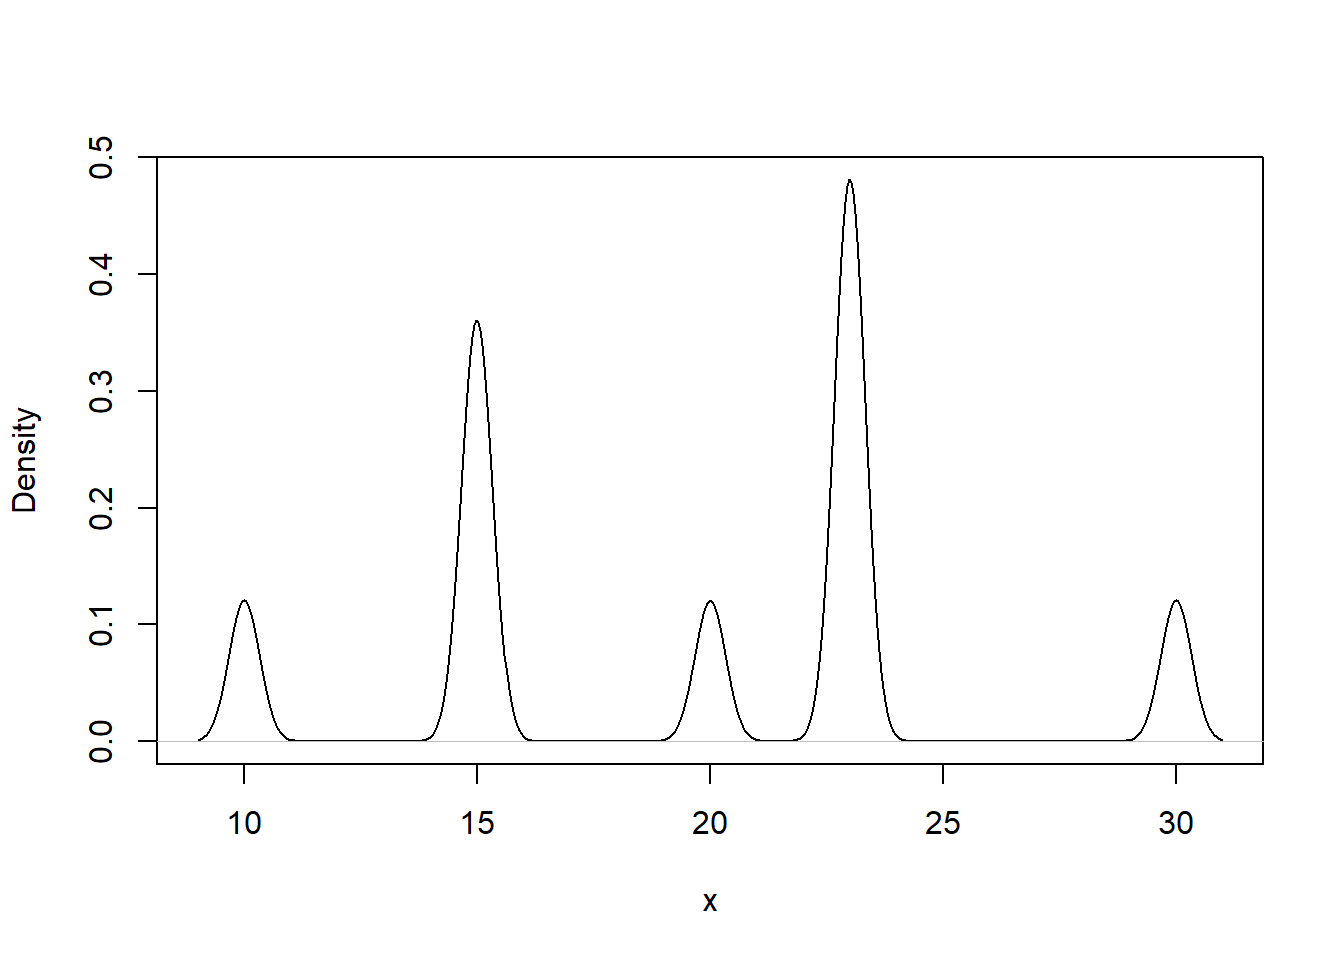
\includegraphics{R_for_Loss_Data_Analytics_files/figure-latex/unnamed-chunk-63-2} \end{center}

\begin{Shaded}
\begin{Highlighting}[]
\KeywordTok{plot}\NormalTok{(}\KeywordTok{density}\NormalTok{(x_example, }\DataTypeTok{kernel =} \StringTok{"triangular"}\NormalTok{), }\DataTypeTok{main=}\StringTok{""}\NormalTok{, }\DataTypeTok{xlab =} \StringTok{"x"}\NormalTok{)  }\CommentTok{# change the kernel}
\end{Highlighting}
\end{Shaded}

\begin{center}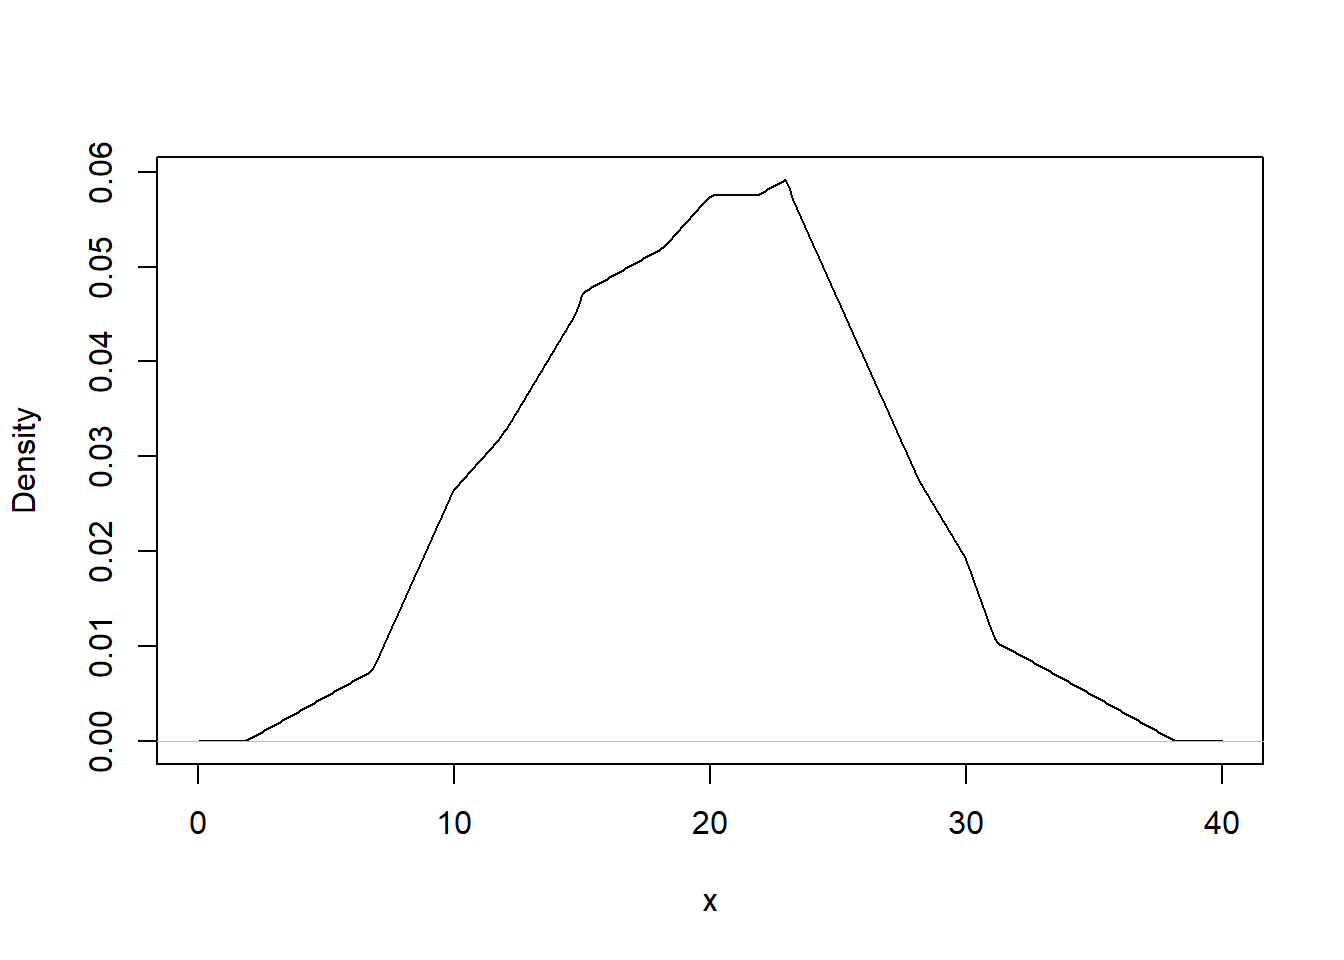
\includegraphics{R_for_Loss_Data_Analytics_files/figure-latex/unnamed-chunk-63-3} \end{center}

\subsection{Property Fund Data}\label{property-fund-data}

This section employs non-parametric estimation tools for model selection
for the claims data of the Property Fund.

\subsubsection{Empirical Distribution Function of Property
Fund}\label{empirical-distribution-function-of-property-fund}

The results below gives the empirical distribution function of the
claims and claims in logarithmic units.

\begin{Shaded}
\begin{Highlighting}[]
\NormalTok{claim_lev <-}\StringTok{ }\KeywordTok{read.csv}\NormalTok{(}\StringTok{"DATA/CLAIMLEVEL.csv"}\NormalTok{, }\DataTypeTok{header=}\OtherTok{TRUE}\NormalTok{)}
\KeywordTok{nrow}\NormalTok{(claim_lev)  }\CommentTok{# 6258}
\end{Highlighting}
\end{Shaded}

\begin{verbatim}
[1] 6258
\end{verbatim}

\begin{Shaded}
\begin{Highlighting}[]
\NormalTok{claim_data <-}\StringTok{ }\KeywordTok{subset}\NormalTok{(claim_lev, Year}\OperatorTok{==}\DecValTok{2010}\NormalTok{)  }\CommentTok{# 2010 subset }
\CommentTok{# Empirical distribution function of Property Fund}
\KeywordTok{par}\NormalTok{(}\DataTypeTok{mfrow =} \KeywordTok{c}\NormalTok{(}\DecValTok{1}\NormalTok{, }\DecValTok{2}\NormalTok{))}
\NormalTok{percentiles  <-}\StringTok{ }\KeywordTok{ecdf}\NormalTok{(claim_data}\OperatorTok{$}\NormalTok{Claim)}
\NormalTok{log_percentiles  <-}\StringTok{ }\KeywordTok{ecdf}\NormalTok{(}\KeywordTok{log}\NormalTok{(claim_data}\OperatorTok{$}\NormalTok{Claim))}
\KeywordTok{plot}\NormalTok{(percentiles,  }\DataTypeTok{main =} \StringTok{""}\NormalTok{, }\DataTypeTok{xlab =} \StringTok{"Claims"}\NormalTok{)}
\KeywordTok{plot}\NormalTok{(log_percentiles, }\DataTypeTok{main =} \StringTok{""}\NormalTok{, }\DataTypeTok{xlab =} \StringTok{"Logarithmic Claims"}\NormalTok{)}
\end{Highlighting}
\end{Shaded}

\begin{center}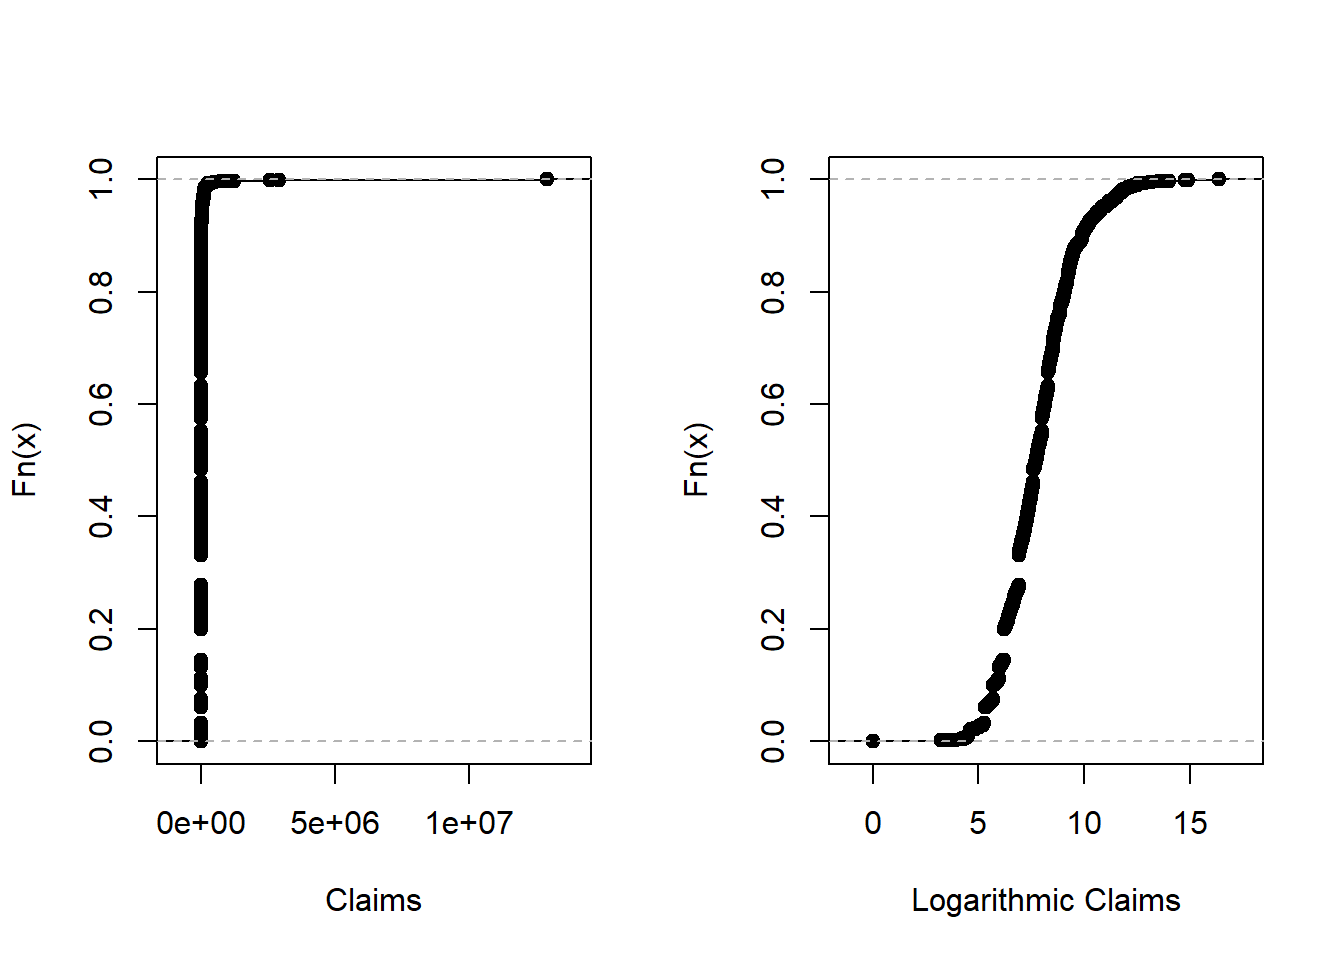
\includegraphics{R_for_Loss_Data_Analytics_files/figure-latex/unnamed-chunk-64-1} \end{center}

\subsubsection{Density Comparison}\label{density-comparison}

Shows a histogram (with shaded gray rectangles) of logarithmic property
claims from 2010. The blue thick curve represents a Gaussian kernel
density where the bandwidth was selected automatically using an ad hoc
rule based on the sample size and volatility of the data.

\begin{Shaded}
\begin{Highlighting}[]
\CommentTok{# Density comparison}
\KeywordTok{hist}\NormalTok{(}\KeywordTok{log}\NormalTok{(claim_data}\OperatorTok{$}\NormalTok{Claim), }\DataTypeTok{main =} \StringTok{""}\NormalTok{, }\DataTypeTok{ylim =} \KeywordTok{c}\NormalTok{(}\DecValTok{0}\NormalTok{, .}\DecValTok{35}\NormalTok{), }\DataTypeTok{xlab =} \StringTok{"Log Expenditures"}\NormalTok{, }
     \DataTypeTok{freq =} \OtherTok{FALSE}\NormalTok{, }\DataTypeTok{col =} \StringTok{"lightgray"}\NormalTok{)}
\KeywordTok{lines}\NormalTok{(}\KeywordTok{density}\NormalTok{(}\KeywordTok{log}\NormalTok{(claim_data}\OperatorTok{$}\NormalTok{Claim)), }\DataTypeTok{col =} \StringTok{"blue"}\NormalTok{, }\DataTypeTok{lwd =} \FloatTok{2.5}\NormalTok{)}
\KeywordTok{lines}\NormalTok{(}\KeywordTok{density}\NormalTok{(}\KeywordTok{log}\NormalTok{(claim_data}\OperatorTok{$}\NormalTok{Claim), }\DataTypeTok{bw =} \DecValTok{1}\NormalTok{), }\DataTypeTok{col =} \StringTok{"green"}\NormalTok{)}
\KeywordTok{lines}\NormalTok{(}\KeywordTok{density}\NormalTok{(}\KeywordTok{log}\NormalTok{(claim_data}\OperatorTok{$}\NormalTok{Claim), }\DataTypeTok{bw =}\NormalTok{ .}\DecValTok{1}\NormalTok{), }\DataTypeTok{col =} \StringTok{"red"}\NormalTok{, }\DataTypeTok{lty =} \DecValTok{3}\NormalTok{)}
\end{Highlighting}
\end{Shaded}

\begin{center}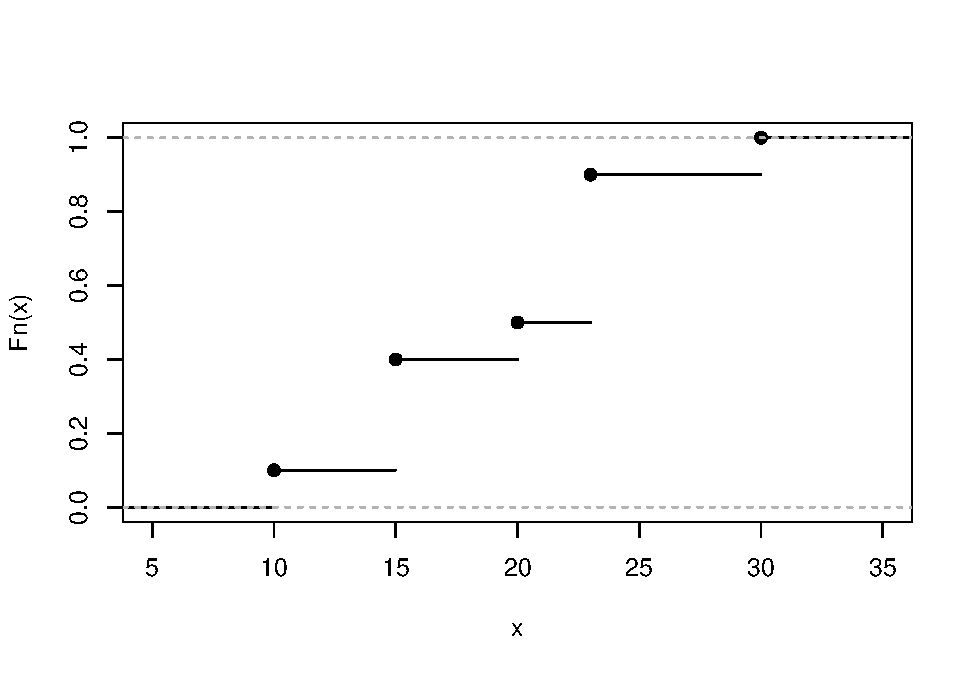
\includegraphics{R_for_Loss_Data_Analytics_files/figure-latex/unnamed-chunk-65-1} \end{center}

\begin{Shaded}
\begin{Highlighting}[]
\KeywordTok{density}\NormalTok{(}\KeywordTok{log}\NormalTok{(claim_data}\OperatorTok{$}\NormalTok{Claim))}\OperatorTok{$}\NormalTok{bw  }\CommentTok{# default bandwidth}
\end{Highlighting}
\end{Shaded}

\begin{verbatim}
[1] 0.3255908
\end{verbatim}

\subsection{Nonparametric Estimation Tools For Model
Selection}\label{nonparametric-estimation-tools-for-model-selection}

\subsubsection{Fit Distributions To The Claims
Data}\label{fit-distributions-to-the-claims-data}

The results below fits gamma and Pareto distribution to the claims data.

\begin{Shaded}
\begin{Highlighting}[]
\KeywordTok{library}\NormalTok{(MASS)}
\KeywordTok{library}\NormalTok{(VGAM)}
\CommentTok{# Inference assuming a gamma distribution}
\NormalTok{fit.gamma_}\DecValTok{2}\NormalTok{ <-}\StringTok{ }\KeywordTok{glm}\NormalTok{(Claim }\OperatorTok{~}\StringTok{ }\DecValTok{1}\NormalTok{, }\DataTypeTok{data =}\NormalTok{ claim_data, }\DataTypeTok{family =} \KeywordTok{Gamma}\NormalTok{(}\DataTypeTok{link =}\NormalTok{ log)) }
\KeywordTok{summary}\NormalTok{(fit.gamma_}\DecValTok{2}\NormalTok{, }\DataTypeTok{dispersion =} \KeywordTok{gamma.dispersion}\NormalTok{(fit.gamma_}\DecValTok{2}\NormalTok{)) }
\end{Highlighting}
\end{Shaded}

\begin{verbatim}

Call:
glm(formula = Claim ~ 1, family = Gamma(link = log), data = claim_data)

Deviance Residuals: 
   Min      1Q  Median      3Q     Max  
-4.287  -2.258  -1.764  -1.178  30.926  

Coefficients:
            Estimate Std. Error z value Pr(>|z|)    
(Intercept) 10.18952    0.04999   203.8   <2e-16 ***
---
Signif. codes:  0 '***' 0.001 '**' 0.01 '*' 0.05 '.' 0.1 ' ' 1

(Dispersion parameter for Gamma family taken to be 3.441204)

    Null deviance: 6569.1  on 1376  degrees of freedom
Residual deviance: 6569.1  on 1376  degrees of freedom
AIC: 28414

Number of Fisher Scoring iterations: 14
\end{verbatim}

\begin{Shaded}
\begin{Highlighting}[]
\NormalTok{( theta <-}\StringTok{ }\KeywordTok{exp}\NormalTok{(}\KeywordTok{coef}\NormalTok{(fit.gamma_}\DecValTok{2}\NormalTok{)) }\OperatorTok{*}\StringTok{ }\KeywordTok{gamma.dispersion}\NormalTok{(fit.gamma_}\DecValTok{2}\NormalTok{))  }\CommentTok{# mu = theta / alpha}
\end{Highlighting}
\end{Shaded}

\begin{verbatim}
(Intercept) 
   91613.78 
\end{verbatim}

\begin{Shaded}
\begin{Highlighting}[]
\NormalTok{( alpha <-}\StringTok{ }\DecValTok{1} \OperatorTok{/}\StringTok{ }\KeywordTok{gamma.dispersion}\NormalTok{(fit.gamma_}\DecValTok{2}\NormalTok{) )}
\end{Highlighting}
\end{Shaded}

\begin{verbatim}
[1] 0.2905959
\end{verbatim}

\begin{Shaded}
\begin{Highlighting}[]
\CommentTok{# Inference assuming a Pareto distribution}
\NormalTok{fit.pareto <-}\StringTok{ }\KeywordTok{vglm}\NormalTok{(Claim }\OperatorTok{~}\StringTok{ }\DecValTok{1}\NormalTok{, paretoII, }\DataTypeTok{loc =} \DecValTok{0}\NormalTok{, }\DataTypeTok{data =}\NormalTok{ claim_data)}
\KeywordTok{summary}\NormalTok{(fit.pareto)}
\end{Highlighting}
\end{Shaded}

\begin{verbatim}

Call:
vglm(formula = Claim ~ 1, family = paretoII, data = claim_data, 
    loc = 0)


Pearson residuals:
                Min      1Q Median     3Q   Max
loge(scale)  -6.332 -0.8289 0.1875 0.8832 1.174
loge(shape) -10.638  0.0946 0.4047 0.4842 0.513

Coefficients: 
                Estimate Std. Error z value Pr(>|z|)    
(Intercept):1  7.7329210  0.0933332  82.853   <2e-16 ***
(Intercept):2 -0.0008753  0.0538642  -0.016    0.987    
---
Signif. codes:  0 '***' 0.001 '**' 0.01 '*' 0.05 '.' 0.1 ' ' 1

Number of linear predictors:  2 

Names of linear predictors: loge(scale), loge(shape)

Log-likelihood: -13404.64 on 2752 degrees of freedom

Number of iterations: 5 

No Hauck-Donner effect found in any of the estimates
\end{verbatim}

\begin{Shaded}
\begin{Highlighting}[]
\KeywordTok{head}\NormalTok{(}\KeywordTok{fitted}\NormalTok{(fit.pareto))}
\end{Highlighting}
\end{Shaded}

\begin{verbatim}
        [,1]
[1,] 2285.03
[2,] 2285.03
[3,] 2285.03
[4,] 2285.03
[5,] 2285.03
[6,] 2285.03
\end{verbatim}

\begin{Shaded}
\begin{Highlighting}[]
\KeywordTok{exp}\NormalTok{(}\KeywordTok{coef}\NormalTok{(fit.pareto))}
\end{Highlighting}
\end{Shaded}

\begin{verbatim}
(Intercept):1 (Intercept):2 
 2282.2590626     0.9991251 
\end{verbatim}

\subsubsection{Graphical Comparison of
Distributions}\label{graphical-comparison-of-distributions}

The graphs below reinforces the technique of overlaying graphs for
comparison purposes using both the distribution function and density
function. Pareto distribution provides a better fit.

\begin{Shaded}
\begin{Highlighting}[]
\CommentTok{# Plotting the fit using densities (on a logarithmic scale)}
\CommentTok{# None of these distributions is doing a great job....}
\NormalTok{x <-}\StringTok{ }\KeywordTok{seq}\NormalTok{(}\DecValTok{0}\NormalTok{, }\DecValTok{15}\NormalTok{, }\DataTypeTok{by =} \FloatTok{0.01}\NormalTok{)}

\KeywordTok{par}\NormalTok{(}\DataTypeTok{mfrow =} \KeywordTok{c}\NormalTok{(}\DecValTok{1}\NormalTok{, }\DecValTok{2}\NormalTok{))}
\NormalTok{log_percentiles  <-}\StringTok{ }\KeywordTok{ecdf}\NormalTok{(}\KeywordTok{log}\NormalTok{(claim_data}\OperatorTok{$}\NormalTok{Claim))}
\KeywordTok{plot}\NormalTok{(log_percentiles,  }\DataTypeTok{main =} \StringTok{""}\NormalTok{, }\DataTypeTok{xlab =} \StringTok{"Claims"}\NormalTok{, }\DataTypeTok{cex =} \FloatTok{0.4}\NormalTok{)}
\NormalTok{Fgamma_ex <-}\StringTok{ }\KeywordTok{pgamma}\NormalTok{(}\KeywordTok{exp}\NormalTok{(x), }\DataTypeTok{shape =}\NormalTok{ alpha, }\DataTypeTok{scale =}\NormalTok{ theta)}
\KeywordTok{lines}\NormalTok{(x, Fgamma_ex, }\DataTypeTok{col =} \StringTok{"blue"}\NormalTok{)}
\NormalTok{Fpareto_ex <-}\StringTok{ }\KeywordTok{pparetoII}\NormalTok{(}\KeywordTok{exp}\NormalTok{(x), }\DataTypeTok{loc =} \DecValTok{0}\NormalTok{,}\DataTypeTok{shape =} \KeywordTok{exp}\NormalTok{(}\KeywordTok{coef}\NormalTok{(fit.pareto)[}\DecValTok{2}\NormalTok{]), }
                        \DataTypeTok{scale =} \KeywordTok{exp}\NormalTok{(}\KeywordTok{coef}\NormalTok{(fit.pareto)[}\DecValTok{1}\NormalTok{]))}
\KeywordTok{lines}\NormalTok{(x, Fpareto_ex, }\DataTypeTok{col =} \StringTok{"purple"}\NormalTok{)}
\KeywordTok{legend}\NormalTok{(}\StringTok{"bottomright"}\NormalTok{, }\KeywordTok{c}\NormalTok{(}\StringTok{"log(claims)"}\NormalTok{, }\StringTok{"Gamma"}\NormalTok{, }\StringTok{"Pareto"}\NormalTok{), }\DataTypeTok{lty =} \DecValTok{1}\NormalTok{, }\DataTypeTok{cex =} \FloatTok{0.6}\NormalTok{, }
       \DataTypeTok{col =} \KeywordTok{c}\NormalTok{(}\StringTok{"black"}\NormalTok{,}\StringTok{"blue"}\NormalTok{,}\StringTok{"purple"}\NormalTok{))}

\KeywordTok{plot}\NormalTok{(}\KeywordTok{density}\NormalTok{(}\KeywordTok{log}\NormalTok{(claim_data}\OperatorTok{$}\NormalTok{Claim)) , }\DataTypeTok{main =} \StringTok{""}\NormalTok{, }\DataTypeTok{xlab =} \StringTok{"Log Expenditures"}\NormalTok{)}
\NormalTok{fgamma_ex <-}\StringTok{ }\KeywordTok{dgamma}\NormalTok{(}\KeywordTok{exp}\NormalTok{(x), }\DataTypeTok{shape =}\NormalTok{ alpha, }\DataTypeTok{scale =}\NormalTok{ theta) }\OperatorTok{*}\StringTok{ }\KeywordTok{exp}\NormalTok{(x)}
\KeywordTok{lines}\NormalTok{(x, fgamma_ex, }\DataTypeTok{col =} \StringTok{"blue"}\NormalTok{)}
\NormalTok{fpareto_ex <-}\StringTok{ }\KeywordTok{dparetoII}\NormalTok{(}\KeywordTok{exp}\NormalTok{(x), }\DataTypeTok{loc =} \DecValTok{0}\NormalTok{, }\DataTypeTok{shape =} \KeywordTok{exp}\NormalTok{(}\KeywordTok{coef}\NormalTok{(fit.pareto)[}\DecValTok{2}\NormalTok{]), }
                        \DataTypeTok{scale =} \KeywordTok{exp}\NormalTok{(}\KeywordTok{coef}\NormalTok{(fit.pareto)[}\DecValTok{1}\NormalTok{])) }\OperatorTok{*}\StringTok{ }\KeywordTok{exp}\NormalTok{(x)}
\KeywordTok{lines}\NormalTok{(x, fpareto_ex, }\DataTypeTok{col =} \StringTok{"purple"}\NormalTok{)}
\KeywordTok{legend}\NormalTok{(}\StringTok{"topright"}\NormalTok{, }\KeywordTok{c}\NormalTok{(}\StringTok{"log(claims)"}\NormalTok{, }\StringTok{"Gamma"}\NormalTok{, }\StringTok{"Pareto"}\NormalTok{), }\DataTypeTok{lty =} \DecValTok{1}\NormalTok{, }\DataTypeTok{cex =} \FloatTok{0.6}\NormalTok{, }
       \DataTypeTok{col =} \KeywordTok{c}\NormalTok{(}\StringTok{"black"}\NormalTok{,}\StringTok{"blue"}\NormalTok{,}\StringTok{"purple"}\NormalTok{))}
\end{Highlighting}
\end{Shaded}

\begin{center}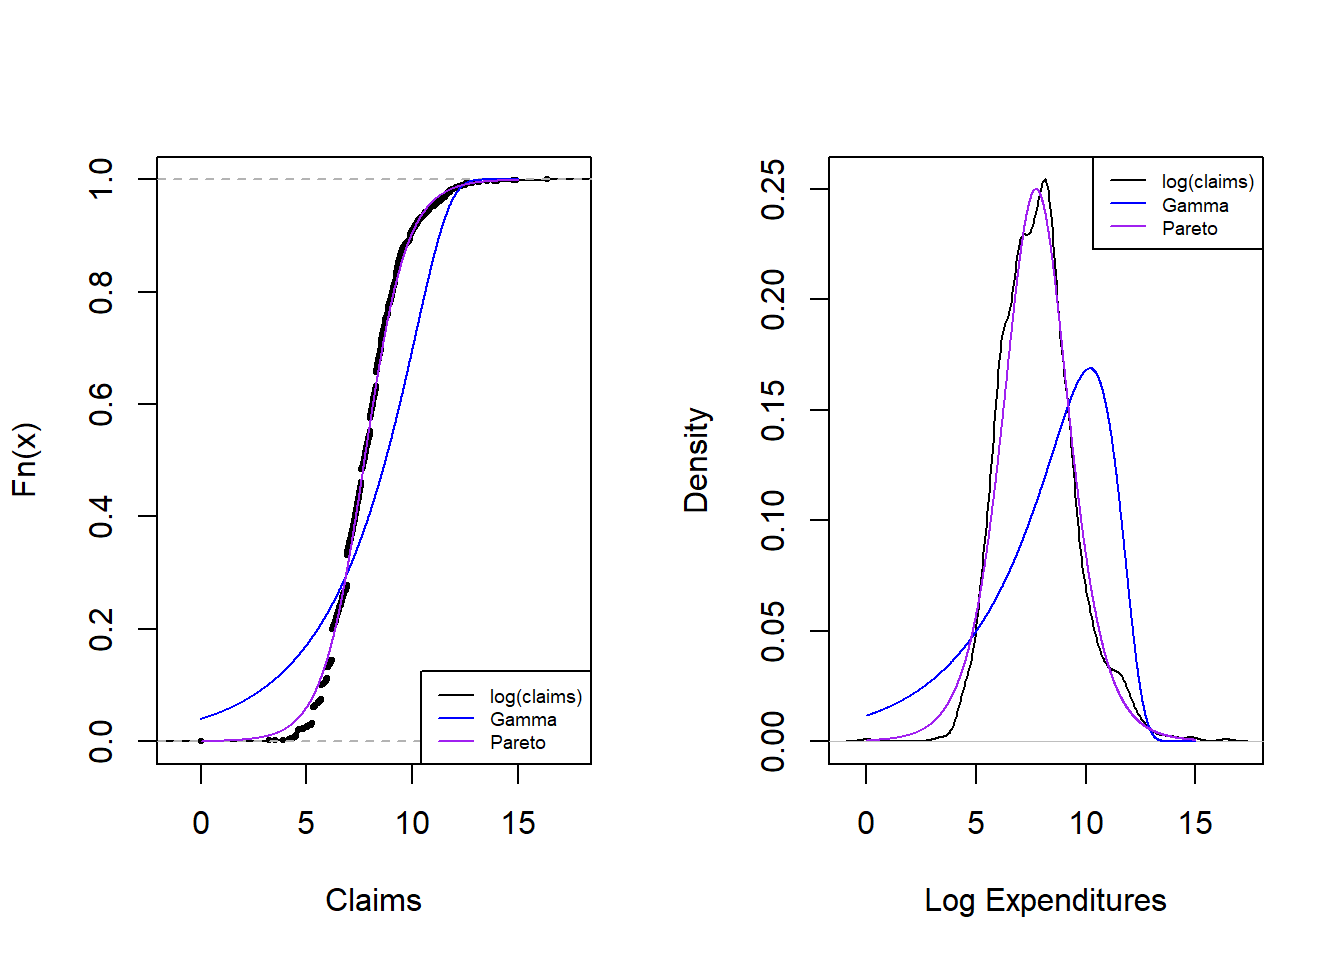
\includegraphics{R_for_Loss_Data_Analytics_files/figure-latex/unnamed-chunk-67-1} \end{center}

\subsubsection{P-P Plots}\label{p-p-plots}

Shows \(pp\) plots for the Property Fund data; the fitted gamma is on
the left and the fitted Pareto is on the right. Pareto distribution
provides a better fit again.

\begin{Shaded}
\begin{Highlighting}[]
\CommentTok{# PP Plot}
\KeywordTok{par}\NormalTok{(}\DataTypeTok{mfrow =} \KeywordTok{c}\NormalTok{(}\DecValTok{1}\NormalTok{, }\DecValTok{2}\NormalTok{))}
\NormalTok{Fgamma_ex <-}\StringTok{ }\KeywordTok{pgamma}\NormalTok{(claim_data}\OperatorTok{$}\NormalTok{Claim, }\DataTypeTok{shape =}\NormalTok{ alpha, }\DataTypeTok{scale =}\NormalTok{ theta)}
\KeywordTok{plot}\NormalTok{(}\KeywordTok{percentiles}\NormalTok{(claim_data}\OperatorTok{$}\NormalTok{Claim), Fgamma_ex, }\DataTypeTok{xlab =} \StringTok{"Empirical DF"}\NormalTok{, }
     \DataTypeTok{ylab =} \StringTok{"Gamma DF"}\NormalTok{, }\DataTypeTok{cex =} \FloatTok{0.4}\NormalTok{)}
\KeywordTok{abline}\NormalTok{(}\DecValTok{0}\NormalTok{, }\DecValTok{1}\NormalTok{)}
\NormalTok{Fpareto_ex <-}\StringTok{ }\KeywordTok{pparetoII}\NormalTok{(claim_data}\OperatorTok{$}\NormalTok{Claim, }\DataTypeTok{loc =} \DecValTok{0}\NormalTok{, }
                        \DataTypeTok{shape =} \KeywordTok{exp}\NormalTok{(}\KeywordTok{coef}\NormalTok{(fit.pareto)[}\DecValTok{2}\NormalTok{]), }
                        \DataTypeTok{scale =} \KeywordTok{exp}\NormalTok{(}\KeywordTok{coef}\NormalTok{(fit.pareto)[}\DecValTok{1}\NormalTok{]))}
\KeywordTok{plot}\NormalTok{(}\KeywordTok{percentiles}\NormalTok{(claim_data}\OperatorTok{$}\NormalTok{Claim), Fpareto_ex, }\DataTypeTok{xlab =} \StringTok{"Empirical DF"}\NormalTok{, }
     \DataTypeTok{ylab =} \StringTok{"Pareto DF"}\NormalTok{, }\DataTypeTok{cex =} \FloatTok{0.4}\NormalTok{)}
\KeywordTok{abline}\NormalTok{(}\DecValTok{0}\NormalTok{, }\DecValTok{1}\NormalTok{)}
\end{Highlighting}
\end{Shaded}

\begin{center}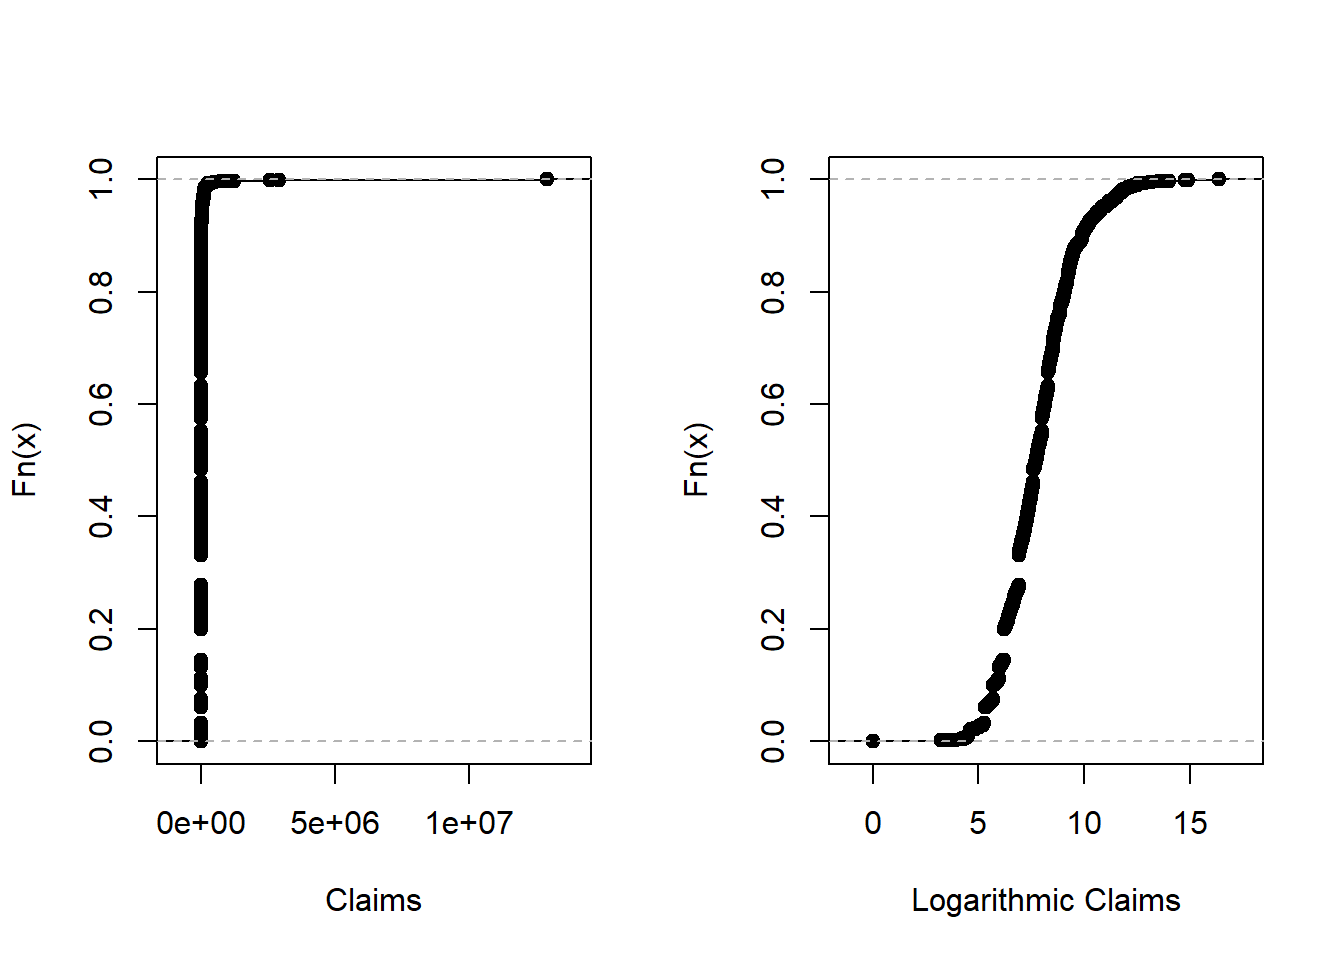
\includegraphics{R_for_Loss_Data_Analytics_files/figure-latex/unnamed-chunk-68-1} \end{center}

\begin{Shaded}
\begin{Highlighting}[]
\CommentTok{#dev.off()}
\end{Highlighting}
\end{Shaded}

\subsubsection{Q-Q Plots}\label{q-q-plots}

In the graphs below the quantiles are plotted on the original scale in
the left-hand panels, on the log scale in the right-hand panel, to allow
the analyst to see where a fitted distribution is deficient.

\begin{Shaded}
\begin{Highlighting}[]
\CommentTok{# Q-Q plot}
\KeywordTok{par}\NormalTok{(}\DataTypeTok{mfrow =} \KeywordTok{c}\NormalTok{(}\DecValTok{2}\NormalTok{, }\DecValTok{2}\NormalTok{))}
\NormalTok{x_seq <-}\StringTok{ }\KeywordTok{seq}\NormalTok{(}\FloatTok{0.0001}\NormalTok{, }\FloatTok{0.9999}\NormalTok{, }\DataTypeTok{by =} \DecValTok{1} \OperatorTok{/}\StringTok{ }\KeywordTok{length}\NormalTok{(claim_data}\OperatorTok{$}\NormalTok{Claim))}
\NormalTok{emp_quant <-}\StringTok{ }\KeywordTok{quantile}\NormalTok{(claim_data}\OperatorTok{$}\NormalTok{Claim, x_seq)}
\NormalTok{gamma_quant <-}\StringTok{ }\KeywordTok{qgamma}\NormalTok{(x_seq, }\DataTypeTok{shape =}\NormalTok{ alpha, }\DataTypeTok{scale =}\NormalTok{ theta)}
\KeywordTok{plot}\NormalTok{(emp_quant, gamma_quant, }\DataTypeTok{xlab =} \StringTok{"Empirical Quantile"}\NormalTok{, }\DataTypeTok{ylab =} \StringTok{"Gamma Quantile"}\NormalTok{)}
\KeywordTok{abline}\NormalTok{(}\DecValTok{0}\NormalTok{, }\DecValTok{1}\NormalTok{)}
\KeywordTok{plot}\NormalTok{(}\KeywordTok{log}\NormalTok{(emp_quant), }\KeywordTok{log}\NormalTok{(gamma_quant), }\DataTypeTok{xlab =} \StringTok{"Log Emp Quantile"}\NormalTok{, }
     \DataTypeTok{ylab =} \StringTok{"Log Gamma Quantile"}\NormalTok{)}
\KeywordTok{abline}\NormalTok{(}\DecValTok{0}\NormalTok{, }\DecValTok{1}\NormalTok{)}
\NormalTok{pareto_quant <-}\StringTok{ }\KeywordTok{qparetoII}\NormalTok{(x_seq, }\DataTypeTok{loc =} \DecValTok{0}\NormalTok{, }\DataTypeTok{shape =} \KeywordTok{exp}\NormalTok{(}\KeywordTok{coef}\NormalTok{(fit.pareto)[}\DecValTok{2}\NormalTok{]), }
                          \DataTypeTok{scale =} \KeywordTok{exp}\NormalTok{(}\KeywordTok{coef}\NormalTok{(fit.pareto)[}\DecValTok{1}\NormalTok{]))}
\KeywordTok{plot}\NormalTok{(emp_quant, pareto_quant, }\DataTypeTok{xlab =} \StringTok{"Empirical Quantile"}\NormalTok{, }\DataTypeTok{ylab =} \StringTok{"Pareto Quantile"}\NormalTok{)}
\KeywordTok{abline}\NormalTok{(}\DecValTok{0}\NormalTok{, }\DecValTok{1}\NormalTok{)}
\KeywordTok{plot}\NormalTok{(}\KeywordTok{log}\NormalTok{(emp_quant), }\KeywordTok{log}\NormalTok{(pareto_quant), }\DataTypeTok{xlab =} \StringTok{"Log Emp Quantile"}\NormalTok{, }
     \DataTypeTok{ylab=}\StringTok{"Log Pareto Quantile"}\NormalTok{)}
\KeywordTok{abline}\NormalTok{(}\DecValTok{0}\NormalTok{, }\DecValTok{1}\NormalTok{)}
\end{Highlighting}
\end{Shaded}

\begin{center}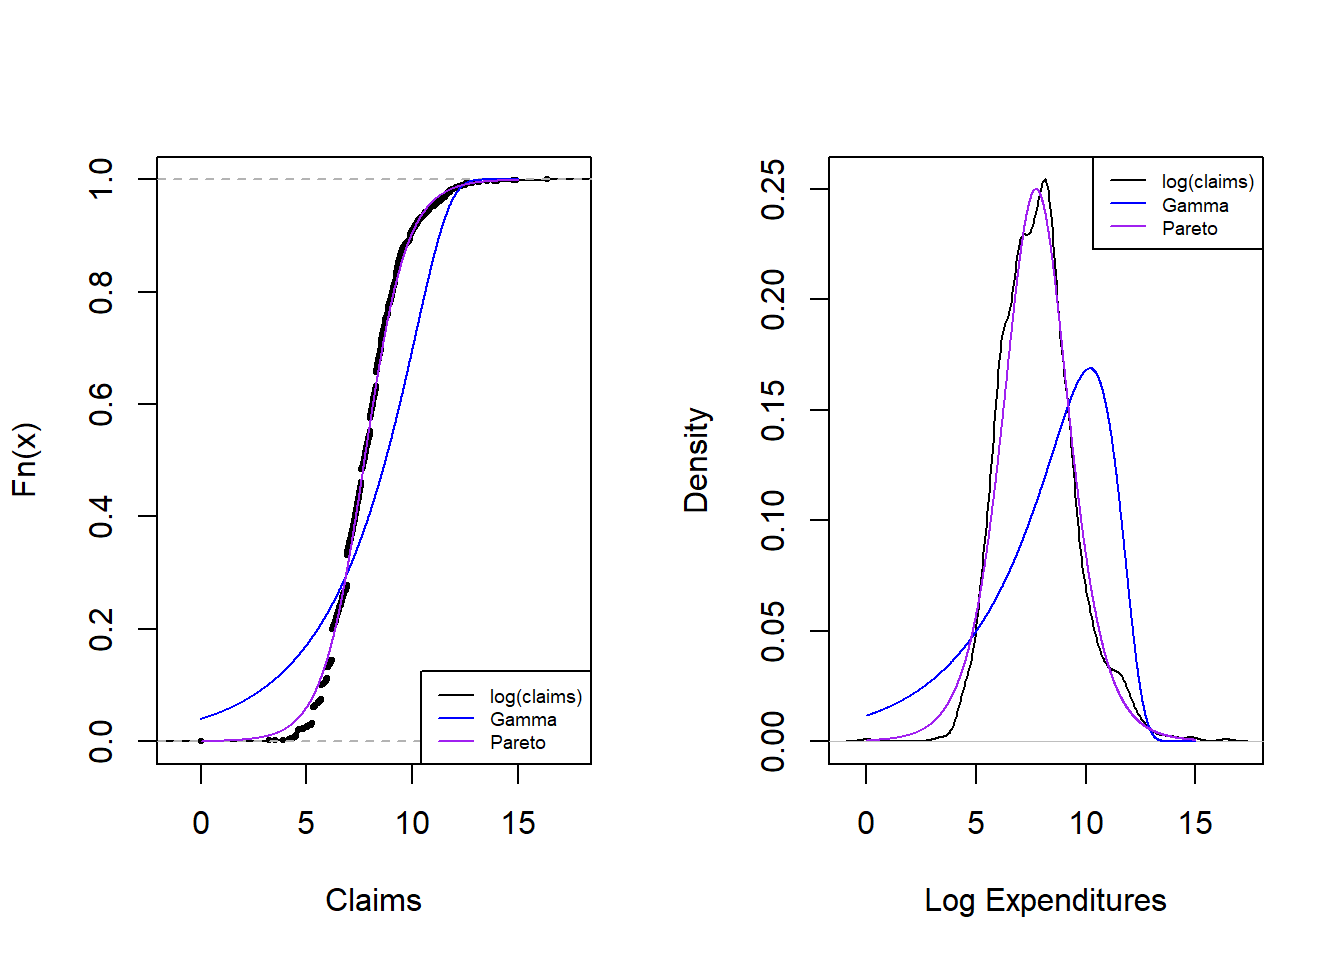
\includegraphics{R_for_Loss_Data_Analytics_files/figure-latex/unnamed-chunk-69-1} \end{center}

\subsubsection{Goodness of Fit
Statistics}\label{goodness-of-fit-statistics}

For reporting results, it can be effective to supplement graphical
displays with selected statistics that summarize model goodness of fit.
The results below provides three commonly used goodness of fit
statistics.

\begin{Shaded}
\begin{Highlighting}[]
\KeywordTok{library}\NormalTok{(goftest)}
\CommentTok{# Kolmogorov-Smirnov # the test statistic is "D"}
\KeywordTok{ks.test}\NormalTok{(claim_data}\OperatorTok{$}\NormalTok{Claim, }\StringTok{"pgamma"}\NormalTok{, }\DataTypeTok{shape =}\NormalTok{ alpha, }\DataTypeTok{scale =}\NormalTok{ theta)}
\end{Highlighting}
\end{Shaded}

\begin{verbatim}

    One-sample Kolmogorov-Smirnov test

data:  claim_data$Claim
D = 0.26387, p-value < 2.2e-16
alternative hypothesis: two-sided
\end{verbatim}

\begin{Shaded}
\begin{Highlighting}[]
\KeywordTok{ks.test}\NormalTok{(claim_data}\OperatorTok{$}\NormalTok{Claim, }\StringTok{"pparetoII"}\NormalTok{, }\DataTypeTok{loc =} \DecValTok{0}\NormalTok{, }\DataTypeTok{shape =} \KeywordTok{exp}\NormalTok{(}\KeywordTok{coef}\NormalTok{(fit.pareto)[}\DecValTok{2}\NormalTok{]), }
        \DataTypeTok{scale =} \KeywordTok{exp}\NormalTok{(}\KeywordTok{coef}\NormalTok{(fit.pareto)[}\DecValTok{1}\NormalTok{]))}
\end{Highlighting}
\end{Shaded}

\begin{verbatim}

    One-sample Kolmogorov-Smirnov test

data:  claim_data$Claim
D = 0.047824, p-value = 0.003677
alternative hypothesis: two-sided
\end{verbatim}

\begin{Shaded}
\begin{Highlighting}[]
\CommentTok{# Cramer-von Mises  # the test statistic is "omega_2"}
\KeywordTok{cvm.test}\NormalTok{(claim_data}\OperatorTok{$}\NormalTok{Claim, }\StringTok{"pgamma"}\NormalTok{, }\DataTypeTok{shape =}\NormalTok{ alpha, }\DataTypeTok{scale =}\NormalTok{ theta)}
\end{Highlighting}
\end{Shaded}

\begin{verbatim}

    Cramer-von Mises test of goodness-of-fit
    Null hypothesis: Gamma distribution
    with parameters shape = 0.290595934110839, scale =
    91613.779421033

data:  claim_data$Claim
omega2 = 33.378, p-value = 2.549e-05
\end{verbatim}

\begin{Shaded}
\begin{Highlighting}[]
\KeywordTok{cvm.test}\NormalTok{(claim_data}\OperatorTok{$}\NormalTok{Claim, }\StringTok{"pparetoII"}\NormalTok{, }\DataTypeTok{loc =} \DecValTok{0}\NormalTok{, }\DataTypeTok{shape =} \KeywordTok{exp}\NormalTok{(}\KeywordTok{coef}\NormalTok{(fit.pareto)[}\DecValTok{2}\NormalTok{]), }
         \DataTypeTok{scale =} \KeywordTok{exp}\NormalTok{(}\KeywordTok{coef}\NormalTok{(fit.pareto)[}\DecValTok{1}\NormalTok{]))}
\end{Highlighting}
\end{Shaded}

\begin{verbatim}

    Cramer-von Mises test of goodness-of-fit
    Null hypothesis: distribution 'pparetoII'
    with parameters shape = 0.999125131378519, scale =
    2282.25906257586

data:  claim_data$Claim
omega2 = 0.38437, p-value = 0.07947
\end{verbatim}

\begin{Shaded}
\begin{Highlighting}[]
\CommentTok{# Anderson-Darling  # the test statistic is "An"}
\KeywordTok{ad.test}\NormalTok{(claim_data}\OperatorTok{$}\NormalTok{Claim, }\StringTok{"pgamma"}\NormalTok{, }\DataTypeTok{shape =}\NormalTok{ alpha, }\DataTypeTok{scale =}\NormalTok{ theta)}
\end{Highlighting}
\end{Shaded}

\begin{verbatim}

    Anderson-Darling test of goodness-of-fit
    Null hypothesis: Gamma distribution
    with parameters shape = 0.290595934110839, scale =
    91613.779421033

data:  claim_data$Claim
An = Inf, p-value = 4.357e-07
\end{verbatim}

\begin{Shaded}
\begin{Highlighting}[]
\KeywordTok{ad.test}\NormalTok{(claim_data}\OperatorTok{$}\NormalTok{Claim, }\StringTok{"pparetoII"}\NormalTok{, }\DataTypeTok{loc =} \DecValTok{0}\NormalTok{, }\DataTypeTok{shape =} \KeywordTok{exp}\NormalTok{(}\KeywordTok{coef}\NormalTok{(fit.pareto)[}\DecValTok{2}\NormalTok{]), }
        \DataTypeTok{scale =} \KeywordTok{exp}\NormalTok{(}\KeywordTok{coef}\NormalTok{(fit.pareto)[}\DecValTok{1}\NormalTok{]))}
\end{Highlighting}
\end{Shaded}

\begin{verbatim}

    Anderson-Darling test of goodness-of-fit
    Null hypothesis: distribution 'pparetoII'
    with parameters shape = 0.999125131378519, scale =
    2282.25906257586

data:  claim_data$Claim
An = 4.1264, p-value = 0.007567
\end{verbatim}

\section{MLE for Grouped Data}\label{mle-for-grouped-data}

\subsection{MLE for Grouped Data- SOA Exam C \#
276}\label{mle-for-grouped-data--soa-exam-c-276}

Losses follow the distribution function \(F(x)=1-(\theta/x),\quad x>0\).
A sample of 20 losses resulted in the following:

\begin{longtable}[]{@{}cc@{}}
\toprule
Interval & Number of Losses\tabularnewline
\midrule
\endhead
(0,10{]} & 9\tabularnewline
(10,25{]} & 6\tabularnewline
(25,infinity) & 5\tabularnewline
\bottomrule
\end{longtable}

Calculate the maximum likelihood estimate of \(\theta\).

\begin{Shaded}
\begin{Highlighting}[]
\CommentTok{# Log likelihood function }
\NormalTok{lik_grp <-}\StringTok{ }\ControlFlowTok{function}\NormalTok{ (theta) \{}
\NormalTok{  log_like <-}\StringTok{ }\KeywordTok{log}\NormalTok{(((}\DecValTok{1} \OperatorTok{-}\StringTok{ }\NormalTok{(theta }\OperatorTok{/}\StringTok{ }\DecValTok{10}\NormalTok{))}\OperatorTok{^}\DecValTok{9}\NormalTok{) }\OperatorTok{*}\StringTok{ }\NormalTok{(((theta }\OperatorTok{/}\StringTok{ }\DecValTok{10}\NormalTok{) }\OperatorTok{-}\StringTok{ }\NormalTok{(theta }\OperatorTok{/}\StringTok{ }\DecValTok{25}\NormalTok{))}\OperatorTok{^}\DecValTok{6}\NormalTok{) }\OperatorTok{*}\StringTok{  }
\StringTok{                   }\NormalTok{(((theta }\OperatorTok{/}\StringTok{ }\DecValTok{25}\NormalTok{))}\OperatorTok{^}\DecValTok{5}\NormalTok{))}
  \KeywordTok{return}\NormalTok{(}\OperatorTok{-}\KeywordTok{sum}\NormalTok{(log_like))}
\NormalTok{\}}
\CommentTok{# "optim" is a general purpose minimization function}
\NormalTok{grp_lik <-}\StringTok{ }\KeywordTok{optim}\NormalTok{(}\KeywordTok{c}\NormalTok{(}\DecValTok{1}\NormalTok{), lik_grp, }\DataTypeTok{method =} \KeywordTok{c}\NormalTok{(}\StringTok{"L-BFGS-B"}\NormalTok{), }\DataTypeTok{hessian =} \OtherTok{TRUE}\NormalTok{)}
\CommentTok{# Estimates - Answer "B" on SoA Problem}
\NormalTok{grp_lik}\OperatorTok{$}\NormalTok{par}
\end{Highlighting}
\end{Shaded}

\begin{verbatim}
[1] 5.5
\end{verbatim}

\begin{Shaded}
\begin{Highlighting}[]
\CommentTok{# Standard error}
\KeywordTok{sqrt}\NormalTok{(}\KeywordTok{diag}\NormalTok{(}\KeywordTok{solve}\NormalTok{(grp_lik}\OperatorTok{$}\NormalTok{hessian)))}
\end{Highlighting}
\end{Shaded}

\begin{verbatim}
[1] 1.11243
\end{verbatim}

\begin{Shaded}
\begin{Highlighting}[]
\CommentTok{# t-statistics}
\NormalTok{( tstat <-}\StringTok{ }\NormalTok{grp_lik}\OperatorTok{$}\NormalTok{par }\OperatorTok{/}\StringTok{ }\KeywordTok{sqrt}\NormalTok{(}\KeywordTok{diag}\NormalTok{(}\KeywordTok{solve}\NormalTok{(grp_lik}\OperatorTok{$}\NormalTok{hessian))) )}
\end{Highlighting}
\end{Shaded}

\begin{verbatim}
[1] 4.944132
\end{verbatim}

\begin{Shaded}
\begin{Highlighting}[]
\CommentTok{# Plot of Negative Log-Likelihood function }
\NormalTok{vllh <-}\StringTok{ }\KeywordTok{Vectorize}\NormalTok{(lik_grp, }\StringTok{"theta"}\NormalTok{)}
\NormalTok{theta <-}\StringTok{ }\KeywordTok{seq}\NormalTok{(}\DecValTok{0}\NormalTok{, }\DecValTok{10}\NormalTok{, }\DataTypeTok{by =} \FloatTok{0.01}\NormalTok{)}
\KeywordTok{plot}\NormalTok{(theta, }\KeywordTok{vllh}\NormalTok{(theta), }\DataTypeTok{pch =} \DecValTok{16}\NormalTok{, }\DataTypeTok{main =} \StringTok{"Negative Log-Likelihood Function"}\NormalTok{, }\DataTypeTok{cex =}\NormalTok{ .}\DecValTok{25}\NormalTok{, }
     \DataTypeTok{xlab =} \KeywordTok{expression}\NormalTok{(theta), }\DataTypeTok{ylab =} \KeywordTok{expression}\NormalTok{(}\KeywordTok{paste}\NormalTok{(}\StringTok{"L("}\NormalTok{, theta, }\StringTok{")"}\NormalTok{)))}
\end{Highlighting}
\end{Shaded}

\begin{center}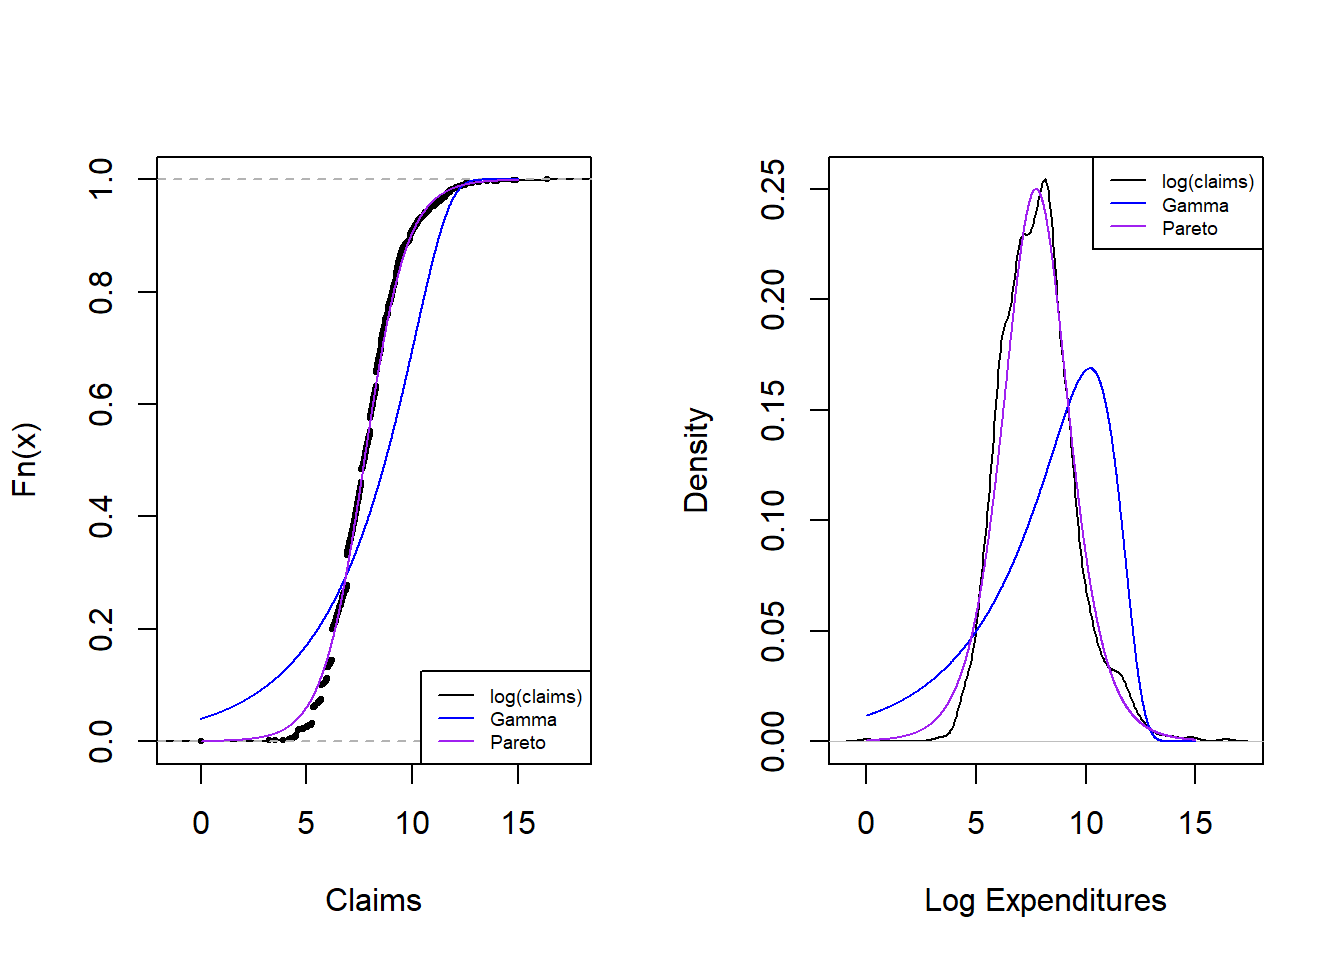
\includegraphics{R_for_Loss_Data_Analytics_files/figure-latex/unnamed-chunk-71-1} \end{center}

\chapter{Simulation}\label{simulation}

\emph{This file contains illustrative \textbf{R} code for computing
important count distributions. When reviewing this code, you should open
an \textbf{R} session, copy-and-paste the code, and see it perform.
Then, you will be able to change parameters, look up commands, and so
forth, as you go. }

\section{Simulation - Inversion
Method}\label{simulation---inversion-method}

This section shows how to use the inversion method to simulate claims
from a gamma distribution. The results below are summary statistics from
the simulated data.

\begin{Shaded}
\begin{Highlighting}[]
\CommentTok{# Simulation - gamma}
\KeywordTok{library}\NormalTok{(moments)}
\KeywordTok{set.seed}\NormalTok{(}\DecValTok{2}\NormalTok{)  }\CommentTok{# set seed to reproduce work }
\NormalTok{n_tot <-}\StringTok{ }\DecValTok{20000}  \CommentTok{# number of simulations}
\NormalTok{alpha <-}\StringTok{ }\DecValTok{2}
\NormalTok{theta <-}\StringTok{ }\DecValTok{100}
         
\NormalTok{losses <-}\StringTok{ }\KeywordTok{rgamma}\NormalTok{(n_tot, alpha, }\DataTypeTok{scale =}\NormalTok{ theta)  }
\KeywordTok{summary}\NormalTok{(losses)}
\end{Highlighting}
\end{Shaded}

\begin{verbatim}
     Min.   1st Qu.    Median      Mean   3rd Qu.      Max. 
   0.0921   96.3265  167.8035  200.1747  268.2257 1110.1298 
\end{verbatim}

\begin{Shaded}
\begin{Highlighting}[]
\NormalTok{k <-}\StringTok{ }\FloatTok{0.95}
\NormalTok{percentile_loss <-}\StringTok{ }\KeywordTok{quantile}\NormalTok{(losses,k)  }\CommentTok{# Kth percentile of losses }
\NormalTok{percentile_loss}
\end{Highlighting}
\end{Shaded}

\begin{verbatim}
     95% 
473.8218 
\end{verbatim}

\begin{Shaded}
\begin{Highlighting}[]
\NormalTok{#######################################}

\CommentTok{# OR you can use this method to simulate losses }
\CommentTok{# Fx <- runif(n_tot)}
\CommentTok{# losses <- qgamma(Fx, alpha, scale = theta)}

\NormalTok{#######################################}

\CommentTok{# For the Pareto Distribution, use}
\CommentTok{# library(VGAM)}
\CommentTok{# n_tot <- 10000  # number of simulations}
\CommentTok{# alpha <- 3}
\CommentTok{# theta <- 25000}
\CommentTok{# losses <- rparetoII(n_tot, scale = theta, shape = alpha)}
\CommentTok{# rparetoII(n_tot, scale = theta, shape = alpha) }
\end{Highlighting}
\end{Shaded}

A few quick notes on these commands:

\begin{itemize}
\tightlist
\item
  The \texttt{rgamma()} function randomly generates data from the Gamma
  distribution. In this illustration the data was generated from a gamma
  distribution with parameters \texttt{shape\ =\ alpha\ =\ 2} and
  \texttt{scale\ =\ theta\ =\ 100}.
\item
  The \texttt{quantile()} function provides sample quantiles
  corresponding to the given probabilities. Here we wanted the simulated
  loss data corresponding to the 95th percentile.
\end{itemize}

\section{Comparing Moments from The Simulated Data to Theoretical
Moments}\label{comparing-moments-from-the-simulated-data-to-theoretical-moments}

\begin{Shaded}
\begin{Highlighting}[]
\KeywordTok{library}\NormalTok{(pander)}
\CommentTok{# Raw moments for k = 0.5}
\CommentTok{# Theoretical }
\NormalTok{k <-}\StringTok{ }\FloatTok{0.5}
\NormalTok{T_}\FloatTok{0.5}\NormalTok{ <-}\StringTok{ }\KeywordTok{round}\NormalTok{(((theta}\OperatorTok{^}\NormalTok{k) }\OperatorTok{*}\StringTok{ }\KeywordTok{gamma}\NormalTok{(alpha }\OperatorTok{+}\StringTok{ }\NormalTok{k)) }\OperatorTok{/}\StringTok{ }\KeywordTok{gamma}\NormalTok{(alpha), }\DecValTok{2}\NormalTok{)}

\CommentTok{# Simulated data raw moments}
\NormalTok{S_}\FloatTok{0.5}\NormalTok{ <-}\StringTok{ }\KeywordTok{round}\NormalTok{(}\KeywordTok{moment}\NormalTok{(losses, }\DataTypeTok{order =}\NormalTok{ k, }\DataTypeTok{central =} \OtherTok{FALSE}\NormalTok{), }\DecValTok{2}\NormalTok{)}


\CommentTok{# Raw moments for k = 1}
\CommentTok{# Theoretical }
\NormalTok{k <-}\StringTok{ }\DecValTok{1}
\NormalTok{T_}\DecValTok{1}\NormalTok{ <-}\StringTok{ }\NormalTok{((theta}\OperatorTok{^}\NormalTok{k) }\OperatorTok{*}\StringTok{ }\KeywordTok{gamma}\NormalTok{(alpha }\OperatorTok{+}\StringTok{ }\NormalTok{k)) }\OperatorTok{/}\StringTok{ }\KeywordTok{gamma}\NormalTok{(alpha)}

\CommentTok{# Simulated data raw moments}
\NormalTok{S_}\DecValTok{1}\NormalTok{ <-}\StringTok{ }\KeywordTok{round}\NormalTok{(}\KeywordTok{moment}\NormalTok{(losses, }\DataTypeTok{order =}\NormalTok{ k, }\DataTypeTok{central =} \OtherTok{FALSE}\NormalTok{), }\DecValTok{2}\NormalTok{)}

\CommentTok{# Raw moments for k = 2}
\CommentTok{# Theoretical }
\NormalTok{k <-}\StringTok{ }\DecValTok{2}
\NormalTok{T_}\DecValTok{2}\NormalTok{ <-}\StringTok{ }\NormalTok{((theta}\OperatorTok{^}\NormalTok{k) }\OperatorTok{*}\StringTok{ }\KeywordTok{gamma}\NormalTok{(alpha }\OperatorTok{+}\StringTok{ }\NormalTok{k)) }\OperatorTok{/}\StringTok{ }\KeywordTok{gamma}\NormalTok{(alpha)}

\CommentTok{#Simulated data raw moments}
\NormalTok{S_}\DecValTok{2}\NormalTok{<-}\KeywordTok{round}\NormalTok{(}\KeywordTok{moment}\NormalTok{(losses, }\DataTypeTok{order =}\NormalTok{ k, }\DataTypeTok{central =} \OtherTok{FALSE}\NormalTok{),}\DecValTok{2}\NormalTok{)}

\CommentTok{# Raw moments for k = 3}
\CommentTok{# Theoretical }
\NormalTok{k <-}\StringTok{ }\DecValTok{3}
\NormalTok{T_}\DecValTok{3}\NormalTok{<-((theta}\OperatorTok{^}\NormalTok{k) }\OperatorTok{*}\StringTok{ }\KeywordTok{gamma}\NormalTok{(alpha }\OperatorTok{+}\StringTok{ }\NormalTok{k)) }\OperatorTok{/}\StringTok{ }\KeywordTok{gamma}\NormalTok{(alpha)}

\CommentTok{# Simulated data raw moments}
\NormalTok{S_}\DecValTok{3}\NormalTok{ <-}\StringTok{ }\KeywordTok{round}\NormalTok{(}\KeywordTok{moment}\NormalTok{(losses, }\DataTypeTok{order =}\NormalTok{ k, }\DataTypeTok{central =} \OtherTok{FALSE}\NormalTok{), }\DecValTok{2}\NormalTok{)}

\CommentTok{# Raw moments for k = 3}

\CommentTok{# Theoretical }
\NormalTok{k <-}\StringTok{ }\DecValTok{4}
\NormalTok{T_}\DecValTok{4}\NormalTok{ <-}\StringTok{ }\NormalTok{((theta}\OperatorTok{^}\NormalTok{k) }\OperatorTok{*}\StringTok{ }\KeywordTok{gamma}\NormalTok{(alpha }\OperatorTok{+}\StringTok{ }\NormalTok{k)) }\OperatorTok{/}\StringTok{ }\KeywordTok{gamma}\NormalTok{(alpha)}

\CommentTok{# Simulated data raw moments}
\NormalTok{S_}\DecValTok{4}\NormalTok{ <-}\StringTok{ }\KeywordTok{round}\NormalTok{(}\KeywordTok{moment}\NormalTok{(losses, }\DataTypeTok{order =}\NormalTok{ k, }\DataTypeTok{central =} \OtherTok{FALSE}\NormalTok{), }\DecValTok{2}\NormalTok{)}

\KeywordTok{pander}\NormalTok{(}\KeywordTok{rbind}\NormalTok{(}\KeywordTok{c}\NormalTok{(}\StringTok{"k"}\NormalTok{, }\FloatTok{0.5}\NormalTok{, }\DecValTok{1}\NormalTok{, }\DecValTok{2}\NormalTok{, }\DecValTok{3}\NormalTok{, }\DecValTok{4}\NormalTok{), }\KeywordTok{c}\NormalTok{(}\StringTok{"Theoretical"}\NormalTok{, T_}\FloatTok{0.5}\NormalTok{, T_}\DecValTok{1}\NormalTok{, T_}\DecValTok{2}\NormalTok{, T_}\DecValTok{3}\NormalTok{, T_}\DecValTok{4}\NormalTok{), }
             \KeywordTok{c}\NormalTok{(}\StringTok{"Simulated"}\NormalTok{, S_}\FloatTok{0.5}\NormalTok{, S_}\DecValTok{1}\NormalTok{, S_}\DecValTok{2}\NormalTok{, S_}\DecValTok{3}\NormalTok{, S_}\DecValTok{4}\NormalTok{)))}
\end{Highlighting}
\end{Shaded}

\begin{longtable}[]{@{}cccccc@{}}
\toprule
\begin{minipage}[t]{0.16\columnwidth}\centering\strut
k\strut
\end{minipage} & \begin{minipage}[t]{0.09\columnwidth}\centering\strut
0.5\strut
\end{minipage} & \begin{minipage}[t]{0.10\columnwidth}\centering\strut
1\strut
\end{minipage} & \begin{minipage}[t]{0.13\columnwidth}\centering\strut
2\strut
\end{minipage} & \begin{minipage}[t]{0.16\columnwidth}\centering\strut
3\strut
\end{minipage} & \begin{minipage}[t]{0.19\columnwidth}\centering\strut
4\strut
\end{minipage}\tabularnewline
\begin{minipage}[t]{0.16\columnwidth}\centering\strut
Theoretical\strut
\end{minipage} & \begin{minipage}[t]{0.09\columnwidth}\centering\strut
13.29\strut
\end{minipage} & \begin{minipage}[t]{0.10\columnwidth}\centering\strut
200\strut
\end{minipage} & \begin{minipage}[t]{0.13\columnwidth}\centering\strut
60000\strut
\end{minipage} & \begin{minipage}[t]{0.16\columnwidth}\centering\strut
2.4e+07\strut
\end{minipage} & \begin{minipage}[t]{0.19\columnwidth}\centering\strut
1.2e+10\strut
\end{minipage}\tabularnewline
\begin{minipage}[t]{0.16\columnwidth}\centering\strut
Simulated\strut
\end{minipage} & \begin{minipage}[t]{0.09\columnwidth}\centering\strut
13.3\strut
\end{minipage} & \begin{minipage}[t]{0.10\columnwidth}\centering\strut
200.17\strut
\end{minipage} & \begin{minipage}[t]{0.13\columnwidth}\centering\strut
60069.73\strut
\end{minipage} & \begin{minipage}[t]{0.16\columnwidth}\centering\strut
23993892.53\strut
\end{minipage} & \begin{minipage}[t]{0.19\columnwidth}\centering\strut
11897735665.89\strut
\end{minipage}\tabularnewline
\bottomrule
\end{longtable}

A few quick notes on these commands:

\begin{itemize}
\tightlist
\item
  The \texttt{moment()} function computes all the sample moments of the
  chosen type up to a given order. In this illustration, we wanted the
  raw sample moments of the \emph{kth} order.
\item
  The \texttt{round()} function was used to round values.
\end{itemize}

\chapter{Aggregate Claim Simulation}\label{aggregate-claim-simulation}

\emph{This file demonstrates simulation of aggregate claim
distributions. When reviewing this code, you should open an \textbf{R}
session, copy-and-paste the code, and see it perform. Then, you will be
able to change parameters, look up commands, and so forth, as you go.}

\section{Collective Risk Model: without coverage
modifications}\label{collective-risk-model-without-coverage-modifications}

S = X\_1 + \ldots{} + X\_N

Assume N \textasciitilde{} Poisson(lambda=2) and X \textasciitilde{}
Pareto(alpha=3,theta=5000)

\subsection{Set Parameters}\label{set-parameters}

\begin{Shaded}
\begin{Highlighting}[]
\NormalTok{lambda <-}\StringTok{ }\DecValTok{2}
\NormalTok{alpha <-}\StringTok{ }\DecValTok{3}
\NormalTok{theta <-}\StringTok{ }\DecValTok{5000}
\end{Highlighting}
\end{Shaded}

\subsection{Show frequency and severity
distributions}\label{show-frequency-and-severity-distributions}

Graphing the our frequency (N) and severity (X) distributions

\begin{Shaded}
\begin{Highlighting}[]
\KeywordTok{par}\NormalTok{(}\DataTypeTok{mfrow=}\KeywordTok{c}\NormalTok{(}\DecValTok{1}\NormalTok{,}\DecValTok{2}\NormalTok{))}

\NormalTok{n <-}\StringTok{ }\DecValTok{1}\OperatorTok{:}\DecValTok{10}
\NormalTok{fn <-}\StringTok{ }\KeywordTok{dpois}\NormalTok{(}\DecValTok{1}\OperatorTok{:}\DecValTok{10}\NormalTok{,lambda)}

\KeywordTok{plot}\NormalTok{(n,fn,}\DataTypeTok{ylim=}\KeywordTok{c}\NormalTok{(}\DecValTok{0}\NormalTok{,}\FloatTok{0.3}\NormalTok{),}\DataTypeTok{main=}\StringTok{"Frequency: Poisson"}\NormalTok{)}
\KeywordTok{abline}\NormalTok{(}\DataTypeTok{h=}\DecValTok{0}\NormalTok{,}\DataTypeTok{lty=}\DecValTok{2}\NormalTok{)}

\NormalTok{x <-}\StringTok{ }\KeywordTok{seq}\NormalTok{(}\DecValTok{1}\NormalTok{,}\DecValTok{25000}\NormalTok{,}\DecValTok{1}\NormalTok{)}
\NormalTok{fx <-}\StringTok{ }\NormalTok{alpha}\OperatorTok{*}\NormalTok{theta}\OperatorTok{^}\NormalTok{alpha}\OperatorTok{/}\NormalTok{(x}\OperatorTok{+}\NormalTok{theta)}\OperatorTok{^}\NormalTok{(alpha}\OperatorTok{+}\DecValTok{1}\NormalTok{)}

\KeywordTok{plot}\NormalTok{(x,fx,}\DataTypeTok{type=}\StringTok{"l"}\NormalTok{,}\DataTypeTok{main=}\StringTok{"Severity: Pareto"}\NormalTok{)}
\end{Highlighting}
\end{Shaded}

\begin{center}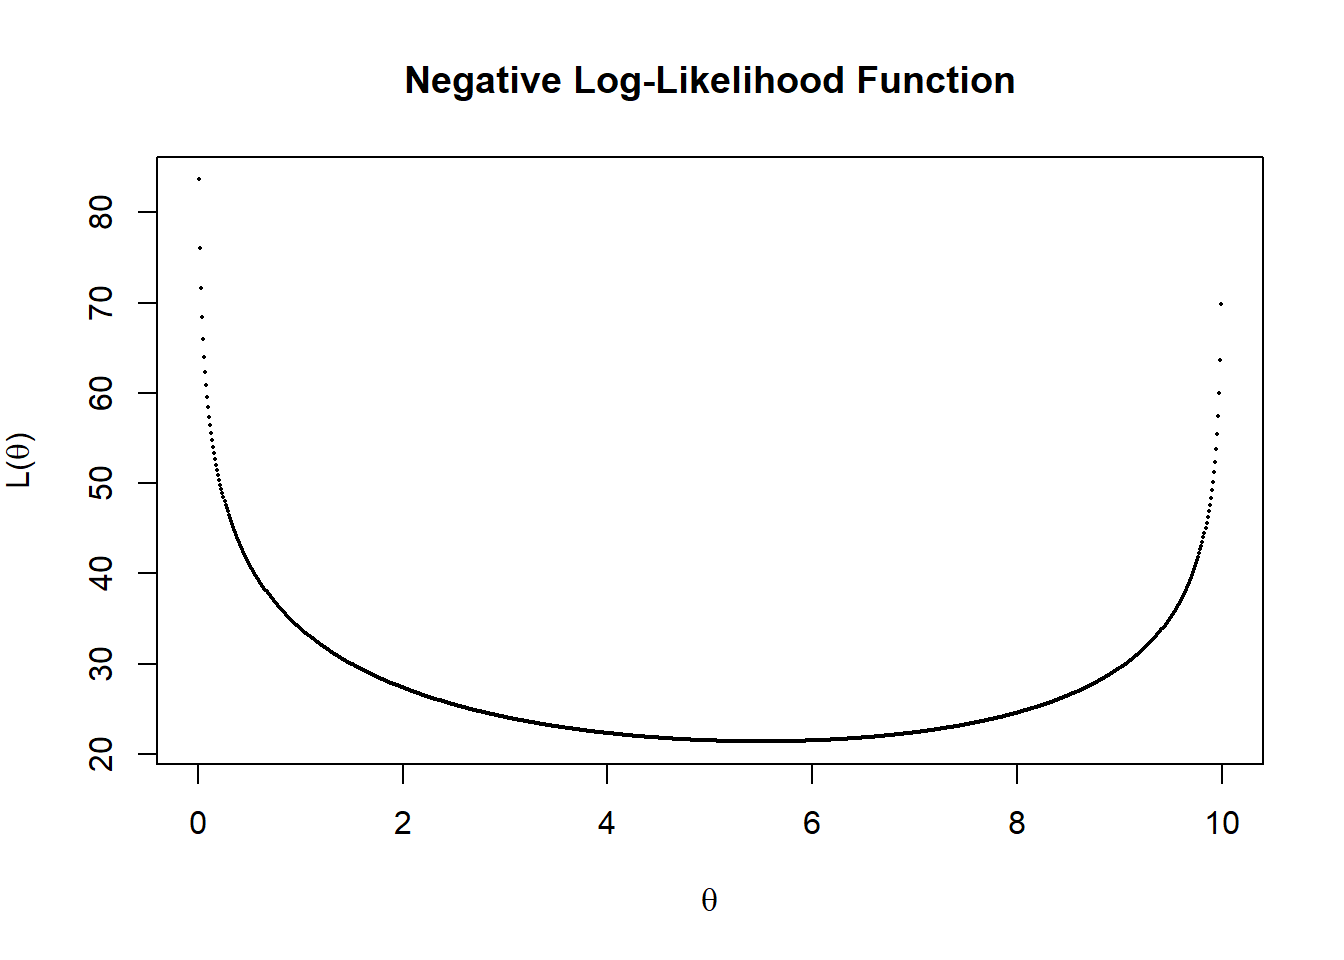
\includegraphics{R_for_Loss_Data_Analytics_files/figure-latex/unnamed-chunk-75-1} \end{center}

\subsection{Set sample size for the
simulation}\label{set-sample-size-for-the-simulation}

We're going to simulate 5000 observations of S

\begin{Shaded}
\begin{Highlighting}[]
\KeywordTok{set.seed}\NormalTok{(}\DecValTok{123}\NormalTok{)}
\NormalTok{size <-}\StringTok{ }\DecValTok{5000}
\NormalTok{S <-}\StringTok{ }\KeywordTok{rep}\NormalTok{(}\OtherTok{NA}\NormalTok{,size)}
\NormalTok{N <-}\StringTok{ }\KeywordTok{rpois}\NormalTok{(size,lambda)}
\ControlFlowTok{for}\NormalTok{ (i }\ControlFlowTok{in} \DecValTok{1}\OperatorTok{:}\NormalTok{size)\{}
\NormalTok{  uu <-}\StringTok{ }\KeywordTok{runif}\NormalTok{(N[i])}
\NormalTok{  X <-}\StringTok{ }\NormalTok{theta}\OperatorTok{*}\NormalTok{((}\DecValTok{1}\OperatorTok{-}\NormalTok{uu)}\OperatorTok{^}\NormalTok{(}\OperatorTok{-}\DecValTok{1}\OperatorTok{/}\NormalTok{alpha)}\OperatorTok{-}\DecValTok{1}\NormalTok{)}
\NormalTok{  S[i] <-}\StringTok{ }\KeywordTok{sum}\NormalTok{(X)}
\NormalTok{\}}
\end{Highlighting}
\end{Shaded}

\subsection{Show distribution of aggregate loss
S}\label{show-distribution-of-aggregate-loss-s}

\begin{Shaded}
\begin{Highlighting}[]
\KeywordTok{par}\NormalTok{(}\DataTypeTok{mfrow=}\KeywordTok{c}\NormalTok{(}\DecValTok{1}\NormalTok{,}\DecValTok{2}\NormalTok{))}
\KeywordTok{hist}\NormalTok{(S,}\DataTypeTok{freq=}\NormalTok{F,}\DataTypeTok{breaks=}\DecValTok{100}\NormalTok{)}
\KeywordTok{plot}\NormalTok{(}\KeywordTok{ecdf}\NormalTok{(S),}\DataTypeTok{xlab=}\StringTok{"S"}\NormalTok{)}
\end{Highlighting}
\end{Shaded}

\begin{center}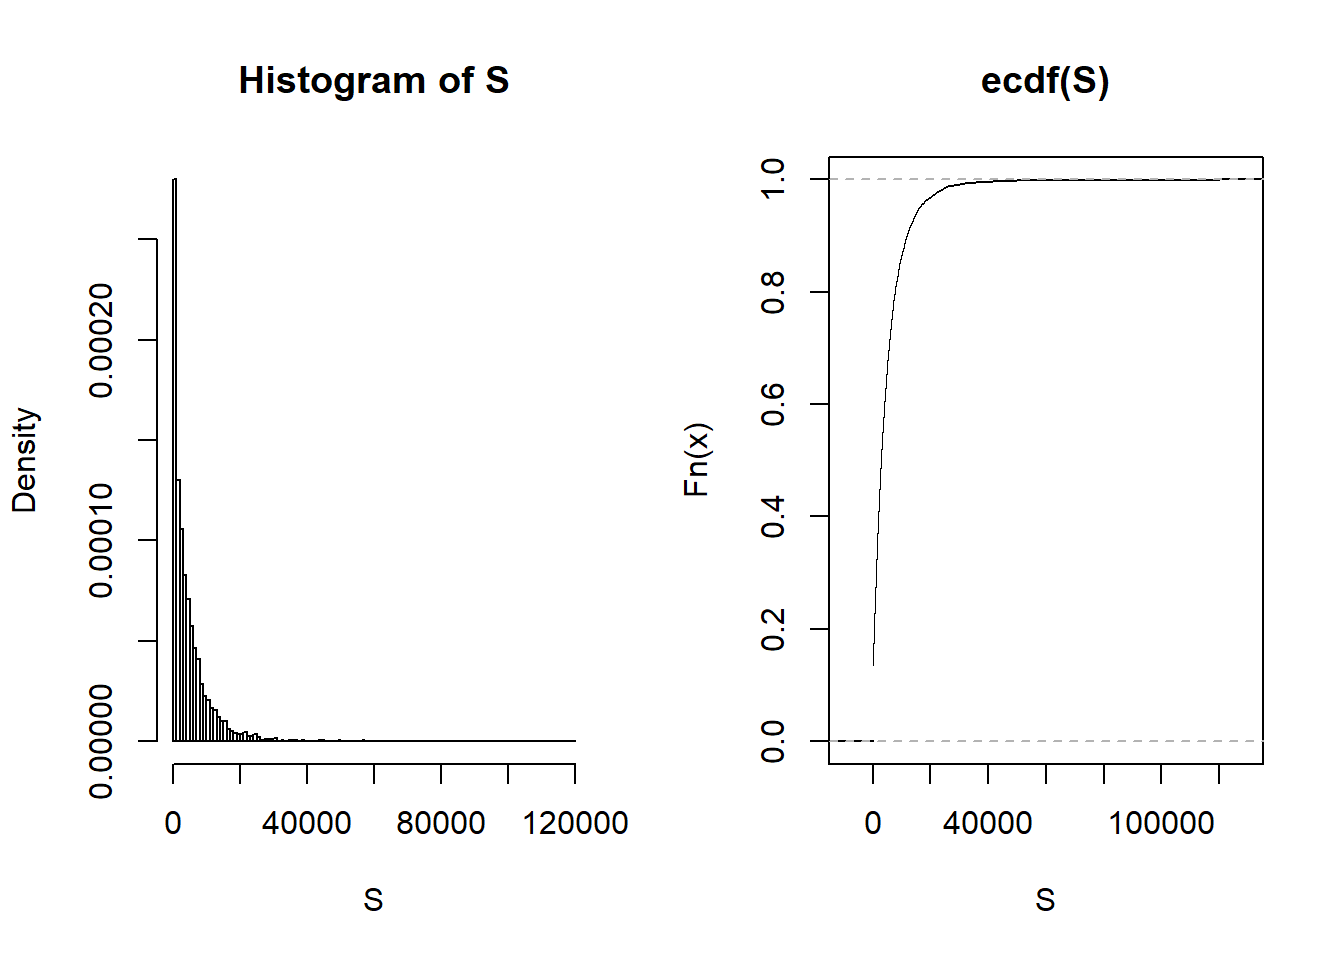
\includegraphics{R_for_Loss_Data_Analytics_files/figure-latex/unnamed-chunk-77-1} \end{center}

\section{Applications}\label{applications}

\subsection{Find descriptive
statistics}\label{find-descriptive-statistics}

Here we show numerical descriptions of our simulated distribution S

\begin{Shaded}
\begin{Highlighting}[]
\KeywordTok{mean}\NormalTok{(S)                             }\CommentTok{# sample mean}
\end{Highlighting}
\end{Shaded}

\begin{verbatim}
[1] 4829.894
\end{verbatim}

\begin{Shaded}
\begin{Highlighting}[]
\KeywordTok{sd}\NormalTok{(S)                               }\CommentTok{# sample standard deviation}
\end{Highlighting}
\end{Shaded}

\begin{verbatim}
[1] 6585.567
\end{verbatim}

\begin{Shaded}
\begin{Highlighting}[]
\KeywordTok{quantile}\NormalTok{(S,}\DataTypeTok{prob=}\KeywordTok{c}\NormalTok{(}\FloatTok{0.05}\NormalTok{,}\FloatTok{0.5}\NormalTok{,}\FloatTok{0.95}\NormalTok{))   }\CommentTok{# percentiles}
\end{Highlighting}
\end{Shaded}

\begin{verbatim}
       5%       50%       95% 
    0.000  2846.073 15983.408 
\end{verbatim}

\subsection{Calculate cdf}\label{calculate-cdf}

\begin{Shaded}
\begin{Highlighting}[]
\KeywordTok{sum}\NormalTok{((S}\OperatorTok{==}\DecValTok{0}\NormalTok{))}\OperatorTok{/}\NormalTok{size}
\end{Highlighting}
\end{Shaded}

\begin{verbatim}
[1] 0.1348
\end{verbatim}

Pr(S=0)

\begin{Shaded}
\begin{Highlighting}[]
\KeywordTok{sum}\NormalTok{(S}\OperatorTok{<=}\KeywordTok{mean}\NormalTok{(S))}\OperatorTok{/}\NormalTok{size}
\end{Highlighting}
\end{Shaded}

\begin{verbatim}
[1] 0.6578
\end{verbatim}

Pr(S\textless{}=E(S))

\begin{Shaded}
\begin{Highlighting}[]
\KeywordTok{sum}\NormalTok{(S}\OperatorTok{>}\KeywordTok{mean}\NormalTok{(S))}\OperatorTok{/}\NormalTok{size }
\end{Highlighting}
\end{Shaded}

\begin{verbatim}
[1] 0.3422
\end{verbatim}

Pr(S\textgreater{}E(S))

\subsection{Calculate risk measures}\label{calculate-risk-measures}

CTE is also known as TVaR

\begin{Shaded}
\begin{Highlighting}[]
\NormalTok{VaR <-}\StringTok{ }\KeywordTok{quantile}\NormalTok{(S,}\DataTypeTok{prob=}\FloatTok{0.99}\NormalTok{)         }\CommentTok{# significance level = 0.01}
\NormalTok{CTE <-}\StringTok{ }\KeywordTok{sum}\NormalTok{(S}\OperatorTok{*}\NormalTok{(S}\OperatorTok{>}\NormalTok{VaR))}\OperatorTok{/}\KeywordTok{sum}\NormalTok{((S}\OperatorTok{>}\NormalTok{VaR))}
\NormalTok{rm <-}\StringTok{ }\KeywordTok{c}\NormalTok{(VaR,CTE)}
\KeywordTok{names}\NormalTok{(rm) <-}\StringTok{ }\KeywordTok{c}\NormalTok{(}\StringTok{"VaR"}\NormalTok{,}\StringTok{"CTE"}\NormalTok{)}
\KeywordTok{print}\NormalTok{(rm)}
\end{Highlighting}
\end{Shaded}

\begin{verbatim}
     VaR      CTE 
28636.56 43193.19 
\end{verbatim}

\subsection{Pricing stop-loss insurance - Set
deductible}\label{pricing-stop-loss-insurance---set-deductible}

Here we plot how the premium for a stop-loss insurance product changes
based on the size of the deductible

\begin{Shaded}
\begin{Highlighting}[]
\KeywordTok{par}\NormalTok{(}\DataTypeTok{mfrow=}\KeywordTok{c}\NormalTok{(}\DecValTok{1}\NormalTok{,}\DecValTok{1}\NormalTok{))}
\NormalTok{d <-}\StringTok{ }\KeywordTok{seq}\NormalTok{(}\DecValTok{0}\NormalTok{,}\DecValTok{120000}\NormalTok{,}\DecValTok{1000}\NormalTok{)}
\NormalTok{price <-}\StringTok{ }\KeywordTok{rep}\NormalTok{(}\OtherTok{NA}\NormalTok{,}\KeywordTok{length}\NormalTok{(d))}
\ControlFlowTok{for}\NormalTok{ (i }\ControlFlowTok{in} \DecValTok{1}\OperatorTok{:}\KeywordTok{length}\NormalTok{(d))\{}
\NormalTok{  price[i] =}\StringTok{ }\KeywordTok{sum}\NormalTok{((S}\OperatorTok{-}\NormalTok{d[i])}\OperatorTok{*}\NormalTok{(S}\OperatorTok{>}\NormalTok{d[i]))}\OperatorTok{/}\NormalTok{size}
\NormalTok{\}}
\KeywordTok{plot}\NormalTok{(d,price,}\DataTypeTok{xlab=}\StringTok{"Deductible"}\NormalTok{,}\DataTypeTok{ylab=}\StringTok{"Stop-Loss Premium"}\NormalTok{,}\DataTypeTok{type=}\StringTok{"b"}\NormalTok{)}
\end{Highlighting}
\end{Shaded}

\begin{center}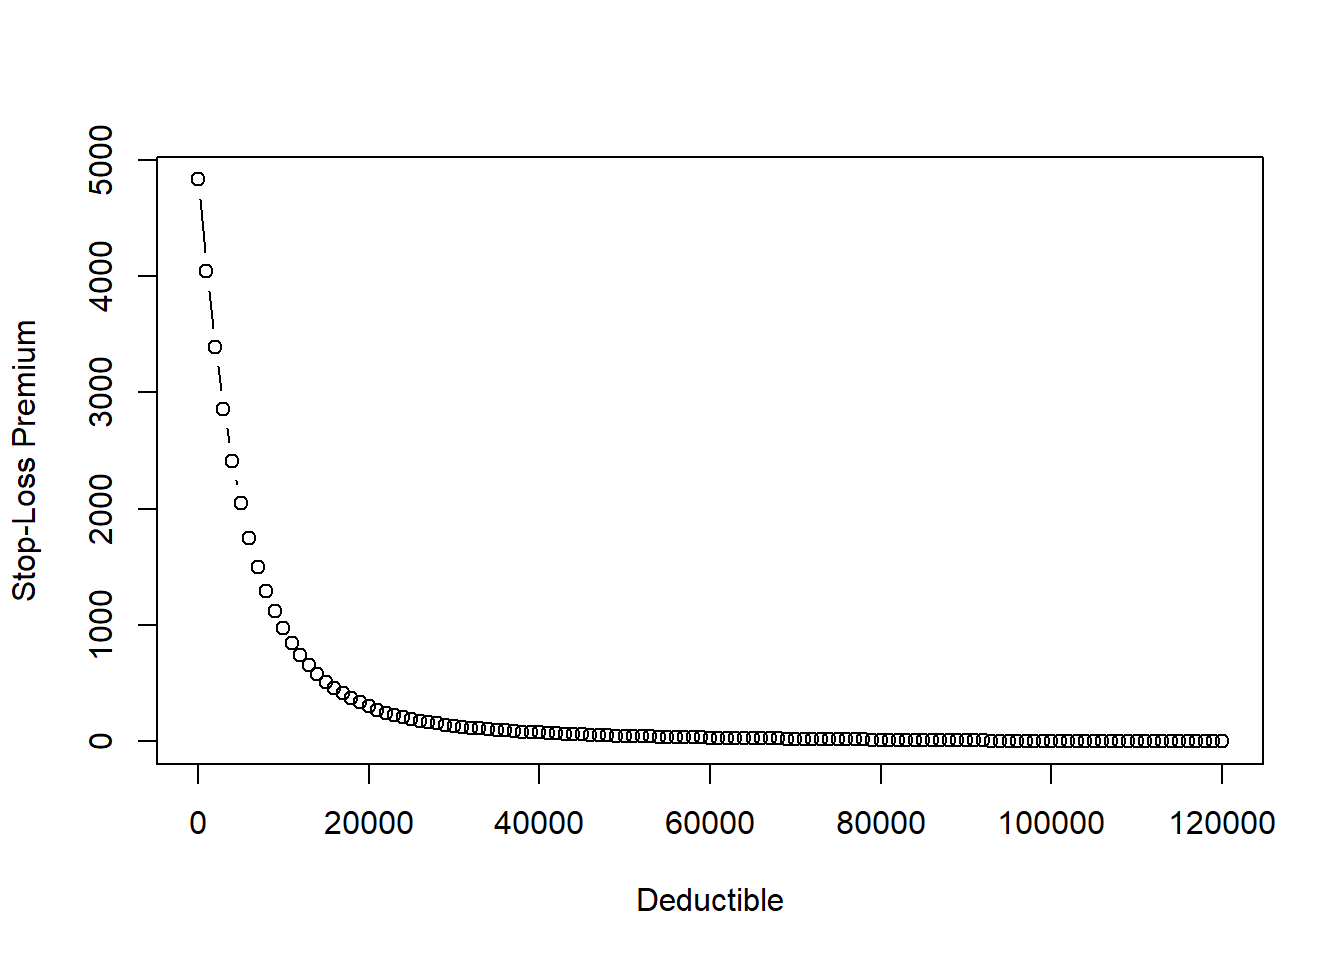
\includegraphics{R_for_Loss_Data_Analytics_files/figure-latex/unnamed-chunk-83-1} \end{center}

\chapter{FreqSev}\label{freqsev}

\emph{This file contains illustrative \textbf{R} code for calculations
involving frequency and severity of distributions. When reviewing this
code, you should open an \textbf{R} session, copy-and-paste the code,
and see it perform. Then, you will be able to change parameters, look up
commands, and so forth, as you go. }

\section{Getting the Data}\label{getting-the-data}

Before we can do any analysis we must import the data.

\subsection{\texorpdfstring{read data
``MassAuto.csv''}{read data MassAuto.csv}}\label{read-data-massauto.csv}

Import the excel file into R.

\begin{Shaded}
\begin{Highlighting}[]
\NormalTok{dat <-}\StringTok{ }\KeywordTok{read.csv}\NormalTok{(}\DataTypeTok{file =} \StringTok{"Data/MassAuto.csv"}\NormalTok{,}\DataTypeTok{header=}\OtherTok{TRUE}\NormalTok{)}
\end{Highlighting}
\end{Shaded}

\subsection{Check Variable Names}\label{check-variable-names}

This code outputs a list of all the variable names of the excel file.
This is useful for determining what kind of data you re working with.

\begin{Shaded}
\begin{Highlighting}[]
\KeywordTok{names}\NormalTok{(dat)}
\end{Highlighting}
\end{Shaded}

\begin{verbatim}
[1] "VIN"       "Territory" "Class"     "Loss1"     "Loss2"    
\end{verbatim}

\subsection{\texorpdfstring{Calculate Total Losses in
``dat''}{Calculate Total Losses in dat}}\label{calculate-total-losses-in-dat}

This code creates a new column representing the sum of the two loss
columns.

\begin{Shaded}
\begin{Highlighting}[]
\NormalTok{dat}\OperatorTok{$}\NormalTok{Loss <-}\StringTok{ }\NormalTok{dat}\OperatorTok{$}\NormalTok{Loss1 }\OperatorTok{+}\StringTok{ }\NormalTok{dat}\OperatorTok{$}\NormalTok{Loss2}
\end{Highlighting}
\end{Shaded}

\section{Fit Frequency Models}\label{fit-frequency-models}

\subsection{Prepare Data for Frequency
Models}\label{prepare-data-for-frequency-models}

You may have to install the package ``dplyr'' to run this code.

\begin{Shaded}
\begin{Highlighting}[]
\KeywordTok{library}\NormalTok{(dplyr)}
\NormalTok{freq.dat <-}\StringTok{ }\NormalTok{dat }\OperatorTok\StringTok{ }\KeywordTok{group_by}\NormalTok{(VIN) }\OperatorTok\StringTok{ }\KeywordTok{summarise}\NormalTok{(}\DataTypeTok{tLoss =} \KeywordTok{sum}\NormalTok{(Loss),}\DataTypeTok{count =} \KeywordTok{sum}\NormalTok{(Loss}\OperatorTok{>}\DecValTok{0}\NormalTok{))}
\KeywordTok{dim}\NormalTok{(freq.dat)}
\end{Highlighting}
\end{Shaded}

\begin{verbatim}
[1] 49894     3
\end{verbatim}

\subsection{Fit Poisson distribution}\label{fit-poisson-distribution}

Here we fit a poisson distrubtion to the data and run log likelihood to
determine the most likely parameter for the distribution. We then
calculate the standard error of this estimate.

\subsubsection{Define the pmf for the Poisson
Distribution}\label{define-the-pmf-for-the-poisson-distribution}

\begin{Shaded}
\begin{Highlighting}[]
\NormalTok{loglikPois<-}\ControlFlowTok{function}\NormalTok{(parms)\{ }
\NormalTok{  lambda=parms[}\DecValTok{1}\NormalTok{]}
\NormalTok{  llk <-}\StringTok{ }\OperatorTok{-}\KeywordTok{sum}\NormalTok{(}\KeywordTok{log}\NormalTok{(}\KeywordTok{dpois}\NormalTok{(freq.dat}\OperatorTok{$}\NormalTok{count,lambda)))}
\NormalTok{  llk}
\NormalTok{\}}
\NormalTok{ini.Pois <-}\StringTok{ }\DecValTok{1}
\NormalTok{zop.Pois <-}\StringTok{ }\KeywordTok{nlminb}\NormalTok{(ini.Pois,loglikPois,}\DataTypeTok{lower=}\KeywordTok{c}\NormalTok{(}\FloatTok{1e-6}\NormalTok{),}\DataTypeTok{upper=}\KeywordTok{c}\NormalTok{(}\OtherTok{Inf}\NormalTok{))}
\KeywordTok{print}\NormalTok{(zop.Pois)}
\end{Highlighting}
\end{Shaded}

\begin{verbatim}
$par
[1] 0.04475488

$objective
[1] 9243.476

$convergence
[1] 0

$iterations
[1] 17

$evaluations
function gradient 
      24       20 

$message
[1] "relative convergence (4)"
\end{verbatim}

\subsubsection{Obtain Standard Error}\label{obtain-standard-error}

\begin{Shaded}
\begin{Highlighting}[]
\KeywordTok{library}\NormalTok{(numDeriv)}
\NormalTok{est <-}\StringTok{ }\NormalTok{zop.Pois}\OperatorTok{$}\NormalTok{par}
\KeywordTok{names}\NormalTok{(est) <-}\StringTok{ }\KeywordTok{c}\NormalTok{(}\StringTok{"lambda"}\NormalTok{)}
\NormalTok{hess<-}\KeywordTok{hessian}\NormalTok{(loglikPois,est)}
\NormalTok{se <-}\KeywordTok{sqrt}\NormalTok{(}\KeywordTok{diag}\NormalTok{(}\KeywordTok{solve}\NormalTok{(hess)))}
\KeywordTok{print}\NormalTok{(}\KeywordTok{cbind}\NormalTok{(est,se))}
\end{Highlighting}
\end{Shaded}

\begin{verbatim}
              est           se
lambda 0.04475488 0.0009471004
\end{verbatim}

\subsection{Fit Negative Binomial
Distribution}\label{fit-negative-binomial-distribution}

Now we fit a negative binomial distribution to the data using log
likelihood.

We then calculate the standard error of this estimate.

\subsubsection{Define pmf for Negative
Binomial}\label{define-pmf-for-negative-binomial}

\begin{Shaded}
\begin{Highlighting}[]
\NormalTok{dnb <-}\StringTok{ }\ControlFlowTok{function}\NormalTok{(y,r,beta)\{}
  \KeywordTok{gamma}\NormalTok{(y}\OperatorTok{+}\NormalTok{r)}\OperatorTok{/}\KeywordTok{gamma}\NormalTok{(r)}\OperatorTok{/}\KeywordTok{gamma}\NormalTok{(y}\OperatorTok{+}\DecValTok{1}\NormalTok{)}\OperatorTok{*}\NormalTok{(}\DecValTok{1}\OperatorTok{/}\NormalTok{(}\DecValTok{1}\OperatorTok{+}\NormalTok{beta))}\OperatorTok{^}\NormalTok{r}\OperatorTok{*}\NormalTok{(beta}\OperatorTok{/}\NormalTok{(}\DecValTok{1}\OperatorTok{+}\NormalTok{beta))}\OperatorTok{^}\NormalTok{y}
\NormalTok{\}}
\NormalTok{loglikNB<-}\ControlFlowTok{function}\NormalTok{(parms)\{ }
\NormalTok{  r=parms[}\DecValTok{1}\NormalTok{]}
\NormalTok{  beta=parms[}\DecValTok{2}\NormalTok{]}
\NormalTok{  llk <-}\StringTok{ }\OperatorTok{-}\KeywordTok{sum}\NormalTok{(}\KeywordTok{log}\NormalTok{(}\KeywordTok{dnb}\NormalTok{(freq.dat}\OperatorTok{$}\NormalTok{count,r,beta)))}
\NormalTok{  llk}
\NormalTok{\}}
\NormalTok{ini.NB <-}\StringTok{ }\KeywordTok{c}\NormalTok{(}\DecValTok{1}\NormalTok{,}\DecValTok{1}\NormalTok{)}
\NormalTok{zop.NB <-}\StringTok{ }\KeywordTok{nlminb}\NormalTok{(ini.NB,loglikNB,}\DataTypeTok{lower=}\KeywordTok{c}\NormalTok{(}\FloatTok{1e-6}\NormalTok{,}\FloatTok{1e-6}\NormalTok{),}\DataTypeTok{upper=}\KeywordTok{c}\NormalTok{(}\OtherTok{Inf}\NormalTok{,}\OtherTok{Inf}\NormalTok{))}
\KeywordTok{print}\NormalTok{(zop.NB)}
\end{Highlighting}
\end{Shaded}

\begin{verbatim}
$par
[1] 0.86573901 0.05169541

$objective
[1] 9218.902

$convergence
[1] 0

$iterations
[1] 27

$evaluations
function gradient 
      32       63 

$message
[1] "relative convergence (4)"
\end{verbatim}

\subsubsection{Obtain Standard Error}\label{obtain-standard-error-1}

\begin{Shaded}
\begin{Highlighting}[]
\KeywordTok{library}\NormalTok{(numDeriv)}
\NormalTok{est <-}\StringTok{ }\NormalTok{zop.NB}\OperatorTok{$}\NormalTok{par}
\KeywordTok{names}\NormalTok{(est) <-}\StringTok{ }\KeywordTok{c}\NormalTok{(}\StringTok{"r"}\NormalTok{,}\StringTok{"beta"}\NormalTok{)}
\NormalTok{hess<-}\KeywordTok{hessian}\NormalTok{(loglikNB,est)}
\NormalTok{se <-}\KeywordTok{sqrt}\NormalTok{(}\KeywordTok{diag}\NormalTok{(}\KeywordTok{solve}\NormalTok{(hess)))}
\KeywordTok{print}\NormalTok{(}\KeywordTok{cbind}\NormalTok{(est,se))}
\end{Highlighting}
\end{Shaded}

\begin{verbatim}
            est          se
r    0.86573901 0.161126426
beta 0.05169541 0.009686412
\end{verbatim}

\subsection{Goodness-of-Fit}\label{goodness-of-fit-1}

Here we calculate goodness of fit for the emipircal, poission, and
negative binomial models.

\subsubsection{Set Parameters}\label{set-parameters-1}

\begin{Shaded}
\begin{Highlighting}[]
\NormalTok{lambda<-zop.Pois}\OperatorTok{$}\NormalTok{par }
\NormalTok{r<-zop.NB}\OperatorTok{$}\NormalTok{par[}\DecValTok{1}\NormalTok{]}
\NormalTok{beta<-zop.NB}\OperatorTok{$}\NormalTok{par[}\DecValTok{2}\NormalTok{]}
\NormalTok{numrow<-}\KeywordTok{max}\NormalTok{(freq.dat}\OperatorTok{$}\NormalTok{count)}\OperatorTok{+}\DecValTok{1}
\end{Highlighting}
\end{Shaded}

\subsubsection{Empirical Model}\label{empirical-model}

\begin{Shaded}
\begin{Highlighting}[]
\NormalTok{emp<-}\KeywordTok{rep}\NormalTok{(}\DecValTok{0}\NormalTok{,numrow}\OperatorTok{+}\DecValTok{1}\NormalTok{)}
\ControlFlowTok{for}\NormalTok{(i }\ControlFlowTok{in} \DecValTok{1}\OperatorTok{:}\NormalTok{(numrow}\OperatorTok{+}\DecValTok{1}\NormalTok{))\{}
\NormalTok{  emp[i]<-}\KeywordTok{sum}\NormalTok{(freq.dat}\OperatorTok{$}\NormalTok{count}\OperatorTok{==}\NormalTok{i}\OperatorTok{-}\DecValTok{1}\NormalTok{)}
\NormalTok{\}}
\end{Highlighting}
\end{Shaded}

\subsubsection{Poisson Model}\label{poisson-model}

\begin{Shaded}
\begin{Highlighting}[]
\NormalTok{pois<-}\KeywordTok{rep}\NormalTok{(}\DecValTok{0}\NormalTok{,numrow}\OperatorTok{+}\DecValTok{1}\NormalTok{)}
\ControlFlowTok{for}\NormalTok{(i }\ControlFlowTok{in} \DecValTok{1}\OperatorTok{:}\NormalTok{numrow)\{}
\NormalTok{  pois[i]<-}\KeywordTok{length}\NormalTok{(freq.dat}\OperatorTok{$}\NormalTok{count)}\OperatorTok{*}\KeywordTok{dpois}\NormalTok{(i}\OperatorTok{-}\DecValTok{1}\NormalTok{,lambda)}
\NormalTok{\}}
\NormalTok{pois[numrow}\OperatorTok{+}\DecValTok{1}\NormalTok{]<-}\StringTok{ }\KeywordTok{length}\NormalTok{(freq.dat}\OperatorTok{$}\NormalTok{count)}\OperatorTok{-}\KeywordTok{sum}\NormalTok{(pois)}
\end{Highlighting}
\end{Shaded}

\subsubsection{Negative Binomial Model}\label{negative-binomial-model}

\begin{Shaded}
\begin{Highlighting}[]
\NormalTok{nb<-}\KeywordTok{rep}\NormalTok{(}\DecValTok{0}\NormalTok{,numrow}\OperatorTok{+}\DecValTok{1}\NormalTok{)}
\ControlFlowTok{for}\NormalTok{(i }\ControlFlowTok{in} \DecValTok{1}\OperatorTok{:}\NormalTok{numrow)\{}
\NormalTok{  nb[i]<-}\KeywordTok{length}\NormalTok{(freq.dat}\OperatorTok{$}\NormalTok{count)}\OperatorTok{*}\KeywordTok{dnb}\NormalTok{(i}\OperatorTok{-}\DecValTok{1}\NormalTok{,r,beta)}
\NormalTok{\}}
\NormalTok{nb[numrow}\OperatorTok{+}\DecValTok{1}\NormalTok{]<-}\StringTok{ }\KeywordTok{length}\NormalTok{(freq.dat}\OperatorTok{$}\NormalTok{count)}\OperatorTok{-}\KeywordTok{sum}\NormalTok{(nb)}
\end{Highlighting}
\end{Shaded}

\subsubsection{Output}\label{output}

\begin{Shaded}
\begin{Highlighting}[]
\NormalTok{freq <-}\StringTok{ }\KeywordTok{cbind}\NormalTok{(emp,pois,nb)}
\KeywordTok{rownames}\NormalTok{(freq) <-}\StringTok{ }\KeywordTok{c}\NormalTok{(}\StringTok{"0"}\NormalTok{,}\StringTok{"1"}\NormalTok{,}\StringTok{"2"}\NormalTok{,}\StringTok{"3"}\NormalTok{,}\StringTok{">3"}\NormalTok{)}
\KeywordTok{colnames}\NormalTok{(freq) <-}\StringTok{ }\KeywordTok{c}\NormalTok{(}\StringTok{"Empirical"}\NormalTok{,}\StringTok{"Poisson"}\NormalTok{,}\StringTok{"NegBin"}\NormalTok{)}
\KeywordTok{round}\NormalTok{(freq,}\DataTypeTok{digits=}\DecValTok{3}\NormalTok{)}
\end{Highlighting}
\end{Shaded}

\begin{verbatim}
   Empirical   Poisson    NegBin
0      47763 47710.232 47763.629
1       2036  2135.266  2032.574
2         88    47.782    93.203
3          7     0.713     4.376
>3         0     0.008     0.218
\end{verbatim}

\subsection{Chi Square Statistics}\label{chi-square-statistics}

Here we run chi square to determine the goodness of fit

\begin{Shaded}
\begin{Highlighting}[]
\NormalTok{chi.pois <-}\StringTok{ }\KeywordTok{sum}\NormalTok{((pois}\OperatorTok{-}\NormalTok{emp)}\OperatorTok{^}\DecValTok{2}\OperatorTok{/}\NormalTok{pois)}
\NormalTok{chi.negbin <-}\StringTok{ }\KeywordTok{sum}\NormalTok{((nb}\OperatorTok{-}\NormalTok{emp)}\OperatorTok{^}\DecValTok{2}\OperatorTok{/}\NormalTok{nb)}
\NormalTok{chisq <-}\StringTok{ }\KeywordTok{c}\NormalTok{(}\DataTypeTok{Poisson=}\NormalTok{chi.pois, }\DataTypeTok{NegBin=}\NormalTok{chi.negbin)}
\KeywordTok{print}\NormalTok{(chisq)}
\end{Highlighting}
\end{Shaded}

\begin{verbatim}
  Poisson    NegBin 
93.986694  2.087543 
\end{verbatim}

\section{Fit Severity Models}\label{fit-severity-models}

\subsection{Prepare Data for Severity
Models}\label{prepare-data-for-severity-models}

\begin{Shaded}
\begin{Highlighting}[]
\NormalTok{sev.dat <-}\StringTok{ }\KeywordTok{subset}\NormalTok{(dat,Loss}\OperatorTok{>}\DecValTok{0}\NormalTok{)}
\KeywordTok{dim}\NormalTok{(sev.dat)}
\end{Highlighting}
\end{Shaded}

\begin{verbatim}
[1] 2233    6
\end{verbatim}

\subsection{Log-normal distribution}\label{log-normal-distribution}

\subsubsection{\texorpdfstring{Use ``VGAM'' Library for Estimation of
Parameters}{Use VGAM Library for Estimation of Parameters}}\label{use-vgam-library-for-estimation-of-parameters}

You may have to install the package ``VGAM'' to run this code.

\begin{Shaded}
\begin{Highlighting}[]
\KeywordTok{library}\NormalTok{(VGAM)}
\NormalTok{fit.LN <-}\StringTok{ }\KeywordTok{vglm}\NormalTok{(Loss }\OperatorTok{~}\StringTok{ }\DecValTok{1}\NormalTok{, }\DataTypeTok{family=}\NormalTok{lognormal, }\DataTypeTok{data =}\NormalTok{ sev.dat)}
\KeywordTok{summary}\NormalTok{(fit.LN)}
\end{Highlighting}
\end{Shaded}

\begin{verbatim}

Call:
vglm(formula = Loss ~ 1, family = lognormal, data = sev.dat)


Pearson residuals:
                Min      1Q   Median      3Q    Max
meanlog     -4.1427 -0.4450  0.05912  0.5917  2.254
loge(sdlog) -0.7071 -0.6636 -0.51680 -0.1437 11.428

Coefficients: 
              Estimate Std. Error z value Pr(>|z|)    
(Intercept):1  7.16870    0.03662  195.76   <2e-16 ***
(Intercept):2  0.54838    0.01496   36.65   <2e-16 ***
---
Signif. codes:  0 '***' 0.001 '**' 0.01 '*' 0.05 '.' 0.1 ' ' 1

Number of linear predictors:  2 

Names of linear predictors: meanlog, loge(sdlog)

Log-likelihood: -20400.73 on 4464 degrees of freedom

Number of iterations: 3 

No Hauck-Donner effect found in any of the estimates
\end{verbatim}

Coefficients (note scale parameter is in log scale).

\begin{Shaded}
\begin{Highlighting}[]
\KeywordTok{coef}\NormalTok{(fit.LN)                }
\end{Highlighting}
\end{Shaded}

\begin{verbatim}
(Intercept):1 (Intercept):2 
    7.1687024     0.5483791 
\end{verbatim}

Confidence intervals for model parameters.

\begin{Shaded}
\begin{Highlighting}[]
\KeywordTok{confint}\NormalTok{(fit.LN, }\DataTypeTok{level=}\FloatTok{0.95}\NormalTok{)   }
\end{Highlighting}
\end{Shaded}

\begin{verbatim}
                  2.5 %    97.5 %
(Intercept):1 7.0969291 7.2404757
(Intercept):2 0.5190507 0.5777076
\end{verbatim}

Loglikelihood for lognormal.

\begin{Shaded}
\begin{Highlighting}[]
\KeywordTok{logLik}\NormalTok{(fit.LN)               }
\end{Highlighting}
\end{Shaded}

\begin{verbatim}
[1] -20400.73
\end{verbatim}

AIC for lognormal.

\begin{Shaded}
\begin{Highlighting}[]
\KeywordTok{AIC}\NormalTok{(fit.LN)                 }
\end{Highlighting}
\end{Shaded}

\begin{verbatim}
[1] 40805.47
\end{verbatim}

BIC for lognormal.

\begin{Shaded}
\begin{Highlighting}[]
\KeywordTok{BIC}\NormalTok{(fit.LN)                 }
\end{Highlighting}
\end{Shaded}

\begin{verbatim}
[1] 40816.89
\end{verbatim}

Covariance matrix for model parameters.

\begin{Shaded}
\begin{Highlighting}[]
\KeywordTok{vcov}\NormalTok{(fit.LN)                 }
\end{Highlighting}
\end{Shaded}

\begin{verbatim}
              (Intercept):1 (Intercept):2
(Intercept):1   0.001341004   0.000000000
(Intercept):2   0.000000000   0.000223914
\end{verbatim}

\subsubsection{User-Defined Likelihood
Function}\label{user-defined-likelihood-function}

Here we estimate sigma directly instead of in log scale.

\begin{Shaded}
\begin{Highlighting}[]
\NormalTok{loglikLN<-}\ControlFlowTok{function}\NormalTok{(parms)\{ }
\NormalTok{  mu=parms[}\DecValTok{1}\NormalTok{]}
\NormalTok{  sigma=parms[}\DecValTok{2}\NormalTok{]}
\NormalTok{  llk <-}\StringTok{ }\OperatorTok{-}\KeywordTok{sum}\NormalTok{(}\KeywordTok{log}\NormalTok{(}\KeywordTok{dlnorm}\NormalTok{(sev.dat}\OperatorTok{$}\NormalTok{Loss, mu, sigma)))}
\NormalTok{  llk}
\NormalTok{\}}
\NormalTok{ini.LN <-}\StringTok{ }\KeywordTok{c}\NormalTok{(}\KeywordTok{coef}\NormalTok{(fit.LN)[}\DecValTok{1}\NormalTok{],}\KeywordTok{exp}\NormalTok{(}\KeywordTok{coef}\NormalTok{(fit.LN)[}\DecValTok{2}\NormalTok{]))}
\NormalTok{zop.LN <-}\StringTok{ }\KeywordTok{nlminb}\NormalTok{(ini.LN,loglikLN,}\DataTypeTok{lower=}\KeywordTok{c}\NormalTok{(}\OperatorTok{-}\OtherTok{Inf}\NormalTok{,}\FloatTok{1e-6}\NormalTok{),}\DataTypeTok{upper=}\KeywordTok{c}\NormalTok{(}\OtherTok{Inf}\NormalTok{,}\OtherTok{Inf}\NormalTok{))}
\KeywordTok{print}\NormalTok{(zop.LN)}
\end{Highlighting}
\end{Shaded}

\begin{verbatim}
$par
(Intercept):1 (Intercept):2 
     7.168702      1.730446 

$objective
[1] 20400.73

$convergence
[1] 0

$iterations
[1] 1

$evaluations
function gradient 
       2        2 

$message
[1] "relative convergence (4)"
\end{verbatim}

\subsubsection{Obtain Standard Error}\label{obtain-standard-error-2}

\begin{Shaded}
\begin{Highlighting}[]
\KeywordTok{library}\NormalTok{(numDeriv)}
\NormalTok{est <-}\StringTok{ }\NormalTok{zop.LN}\OperatorTok{$}\NormalTok{par}
\KeywordTok{names}\NormalTok{(est) <-}\StringTok{ }\KeywordTok{c}\NormalTok{(}\StringTok{"mu"}\NormalTok{,}\StringTok{"sigma"}\NormalTok{)}
\NormalTok{hess<-}\KeywordTok{hessian}\NormalTok{(loglikLN,est)}
\NormalTok{se <-}\KeywordTok{sqrt}\NormalTok{(}\KeywordTok{diag}\NormalTok{(}\KeywordTok{solve}\NormalTok{(hess)))}
\KeywordTok{print}\NormalTok{(}\KeywordTok{cbind}\NormalTok{(est,se))}
\end{Highlighting}
\end{Shaded}

\begin{verbatim}
           est         se
mu    7.168702 0.03661961
sigma 1.730446 0.02589397
\end{verbatim}

\subsection{Pareto Distribution}\label{pareto-distribution-1}

\subsubsection{\texorpdfstring{Use ``VGAM'' Library for Estimation of
Parameters}{Use VGAM Library for Estimation of Parameters}}\label{use-vgam-library-for-estimation-of-parameters-1}

You may have to install the package ``VGAM'' to run this code.

\begin{Shaded}
\begin{Highlighting}[]
\KeywordTok{library}\NormalTok{(VGAM)}
\NormalTok{fit.pareto <-}\StringTok{ }\KeywordTok{vglm}\NormalTok{(Loss }\OperatorTok{~}\StringTok{ }\DecValTok{1}\NormalTok{, paretoII, }\DataTypeTok{loc=}\DecValTok{0}\NormalTok{, }\DataTypeTok{data =}\NormalTok{ sev.dat)}
\KeywordTok{summary}\NormalTok{(fit.pareto)}
\end{Highlighting}
\end{Shaded}

\begin{verbatim}

Call:
vglm(formula = Loss ~ 1, family = paretoII, data = sev.dat, loc = 0)


Pearson residuals:
               Min      1Q  Median     3Q    Max
loge(scale) -2.044 -0.7540 0.02541 0.8477 1.2958
loge(shape) -5.813  0.1526 0.36197 0.4322 0.4559

Coefficients: 
              Estimate Std. Error z value Pr(>|z|)    
(Intercept):1  7.99629    0.08417  95.004   <2e-16 ***
(Intercept):2  0.52653    0.05699   9.239   <2e-16 ***
---
Signif. codes:  0 '***' 0.001 '**' 0.01 '*' 0.05 '.' 0.1 ' ' 1

Number of linear predictors:  2 

Names of linear predictors: loge(scale), loge(shape)

Log-likelihood: -20231.91 on 4464 degrees of freedom

Number of iterations: 5 

No Hauck-Donner effect found in any of the estimates
\end{verbatim}

\begin{Shaded}
\begin{Highlighting}[]
\KeywordTok{head}\NormalTok{(}\KeywordTok{fitted}\NormalTok{(fit.pareto))}
\end{Highlighting}
\end{Shaded}

\begin{verbatim}
         [,1]
[1,] 1502.569
[2,] 1502.569
[3,] 1502.569
[4,] 1502.569
[5,] 1502.569
[6,] 1502.569
\end{verbatim}

\begin{Shaded}
\begin{Highlighting}[]
\KeywordTok{coef}\NormalTok{(fit.pareto)                 }\CommentTok{#note both parameters are in log scale}
\end{Highlighting}
\end{Shaded}

\begin{verbatim}
(Intercept):1 (Intercept):2 
    7.9962932     0.5265276 
\end{verbatim}

\begin{Shaded}
\begin{Highlighting}[]
\KeywordTok{exp}\NormalTok{(}\KeywordTok{coef}\NormalTok{(fit.pareto))            }\CommentTok{#estimate of parameters}
\end{Highlighting}
\end{Shaded}

\begin{verbatim}
(Intercept):1 (Intercept):2 
  2969.928635      1.693043 
\end{verbatim}

\begin{Shaded}
\begin{Highlighting}[]
\KeywordTok{confint}\NormalTok{(fit.pareto, }\DataTypeTok{level=}\FloatTok{0.95}\NormalTok{)  }\CommentTok{#confidence intervals for model parameters }
\end{Highlighting}
\end{Shaded}

\begin{verbatim}
                 2.5 %    97.5 %
(Intercept):1 7.831327 8.1612593
(Intercept):2 0.414834 0.6382213
\end{verbatim}

\begin{Shaded}
\begin{Highlighting}[]
\KeywordTok{logLik}\NormalTok{(fit.pareto)               }\CommentTok{#loglikelihood for pareto}
\end{Highlighting}
\end{Shaded}

\begin{verbatim}
[1] -20231.91
\end{verbatim}

\begin{Shaded}
\begin{Highlighting}[]
\KeywordTok{AIC}\NormalTok{(fit.pareto)                  }\CommentTok{#AIC for pareto}
\end{Highlighting}
\end{Shaded}

\begin{verbatim}
[1] 40467.83
\end{verbatim}

\begin{Shaded}
\begin{Highlighting}[]
\KeywordTok{BIC}\NormalTok{(fit.pareto)                  }\CommentTok{#BIC for pareto}
\end{Highlighting}
\end{Shaded}

\begin{verbatim}
[1] 40479.25
\end{verbatim}

\begin{Shaded}
\begin{Highlighting}[]
\KeywordTok{vcov}\NormalTok{(fit.pareto)                 }\CommentTok{#covariance matrix for model parameters }
\end{Highlighting}
\end{Shaded}

\begin{verbatim}
              (Intercept):1 (Intercept):2
(Intercept):1   0.007084237   0.004453555
(Intercept):2   0.004453555   0.003247586
\end{verbatim}

\subsubsection{User-Defined Likelihood
Function}\label{user-defined-likelihood-function-1}

Here we estimate alpha and theta directly to define the pareto density.

\begin{Shaded}
\begin{Highlighting}[]
\NormalTok{dpareto <-}\StringTok{ }\ControlFlowTok{function}\NormalTok{(y,theta,alpha)\{}
\NormalTok{  alpha}\OperatorTok{*}\NormalTok{theta}\OperatorTok{^}\NormalTok{alpha}\OperatorTok{/}\NormalTok{(y}\OperatorTok{+}\NormalTok{theta)}\OperatorTok{^}\NormalTok{(alpha}\OperatorTok{+}\DecValTok{1}\NormalTok{)}
\NormalTok{\}}
\NormalTok{loglikP<-}\ControlFlowTok{function}\NormalTok{(parms)\{ }
\NormalTok{  theta=parms[}\DecValTok{1}\NormalTok{]}
\NormalTok{  alpha=parms[}\DecValTok{2}\NormalTok{]}
\NormalTok{  llk <-}\StringTok{ }\OperatorTok{-}\KeywordTok{sum}\NormalTok{(}\KeywordTok{log}\NormalTok{(}\KeywordTok{dpareto}\NormalTok{(sev.dat}\OperatorTok{$}\NormalTok{Loss,theta,alpha)))}
\NormalTok{  llk}
\NormalTok{\}}
\NormalTok{ini.P <-}\StringTok{ }\KeywordTok{exp}\NormalTok{(}\KeywordTok{coef}\NormalTok{(fit.pareto))}
\NormalTok{zop.P <-}\StringTok{ }\KeywordTok{nlminb}\NormalTok{(ini.P,loglikP,}\DataTypeTok{lower=}\KeywordTok{c}\NormalTok{(}\FloatTok{1e-6}\NormalTok{,}\FloatTok{1e-6}\NormalTok{),}\DataTypeTok{upper=}\KeywordTok{c}\NormalTok{(}\OtherTok{Inf}\NormalTok{,}\OtherTok{Inf}\NormalTok{))}
\KeywordTok{print}\NormalTok{(zop.P)}
\end{Highlighting}
\end{Shaded}

\begin{verbatim}
$par
(Intercept):1 (Intercept):2 
  2969.928635      1.693043 

$objective
[1] 20231.91

$convergence
[1] 0

$iterations
[1] 1

$evaluations
function gradient 
       1        2 

$message
[1] "both X-convergence and relative convergence (5)"
\end{verbatim}

\subsubsection{Obtain Standard Error}\label{obtain-standard-error-3}

\begin{Shaded}
\begin{Highlighting}[]
\KeywordTok{library}\NormalTok{(numDeriv)}
\NormalTok{est <-}\StringTok{ }\NormalTok{zop.P}\OperatorTok{$}\NormalTok{par}
\KeywordTok{names}\NormalTok{(est) <-}\StringTok{ }\KeywordTok{c}\NormalTok{(}\StringTok{"theta"}\NormalTok{,}\StringTok{"alpha"}\NormalTok{)}
\NormalTok{hess<-}\KeywordTok{hessian}\NormalTok{(loglikP,est)}
\NormalTok{se <-}\KeywordTok{sqrt}\NormalTok{(}\KeywordTok{diag}\NormalTok{(}\KeywordTok{solve}\NormalTok{(hess)))}
\KeywordTok{print}\NormalTok{(}\KeywordTok{cbind}\NormalTok{(est,se))}
\end{Highlighting}
\end{Shaded}

\begin{verbatim}
              est           se
theta 2969.928635 248.24191162
alpha    1.693043   0.09590892
\end{verbatim}

\subsection{Histogram}\label{histogram}

prepare the display window parameters to properly fit the histograms

\begin{Shaded}
\begin{Highlighting}[]
\KeywordTok{par}\NormalTok{(}\DataTypeTok{mfrow=}\KeywordTok{c}\NormalTok{(}\DecValTok{1}\NormalTok{,}\DecValTok{2}\NormalTok{))}
\end{Highlighting}
\end{Shaded}

\subsubsection{LN}\label{ln}

\begin{Shaded}
\begin{Highlighting}[]
\KeywordTok{hist}\NormalTok{(sev.dat}\OperatorTok{$}\NormalTok{Loss,}\DataTypeTok{xlab=}\StringTok{"Total Losses"}\NormalTok{,}\DataTypeTok{main=}\StringTok{"LN"}\NormalTok{,}\DataTypeTok{breaks=}\DecValTok{100}\NormalTok{,}\DataTypeTok{freq=}\NormalTok{F,}\DataTypeTok{xlim=}\KeywordTok{c}\NormalTok{(}\DecValTok{0}\NormalTok{,}\FloatTok{3e4}\NormalTok{),}\DataTypeTok{ylim=}\KeywordTok{c}\NormalTok{(}\DecValTok{0}\NormalTok{,}\FloatTok{8e-4}\NormalTok{))}
\NormalTok{x <-}\StringTok{ }\KeywordTok{seq}\NormalTok{(}\DecValTok{1}\NormalTok{,}\KeywordTok{max}\NormalTok{(sev.dat}\OperatorTok{$}\NormalTok{Loss),}\DecValTok{1}\NormalTok{)}
\NormalTok{mu <-}\StringTok{ }\NormalTok{zop.LN}\OperatorTok{$}\NormalTok{par[}\DecValTok{1}\NormalTok{]}
\NormalTok{sigma <-}\StringTok{ }\NormalTok{zop.LN}\OperatorTok{$}\NormalTok{par[}\DecValTok{2}\NormalTok{]}
\KeywordTok{lines}\NormalTok{(x,}\KeywordTok{dlnorm}\NormalTok{(x,mu,sigma),}\DataTypeTok{col=}\StringTok{"red"}\NormalTok{)}
\end{Highlighting}
\end{Shaded}

\begin{center}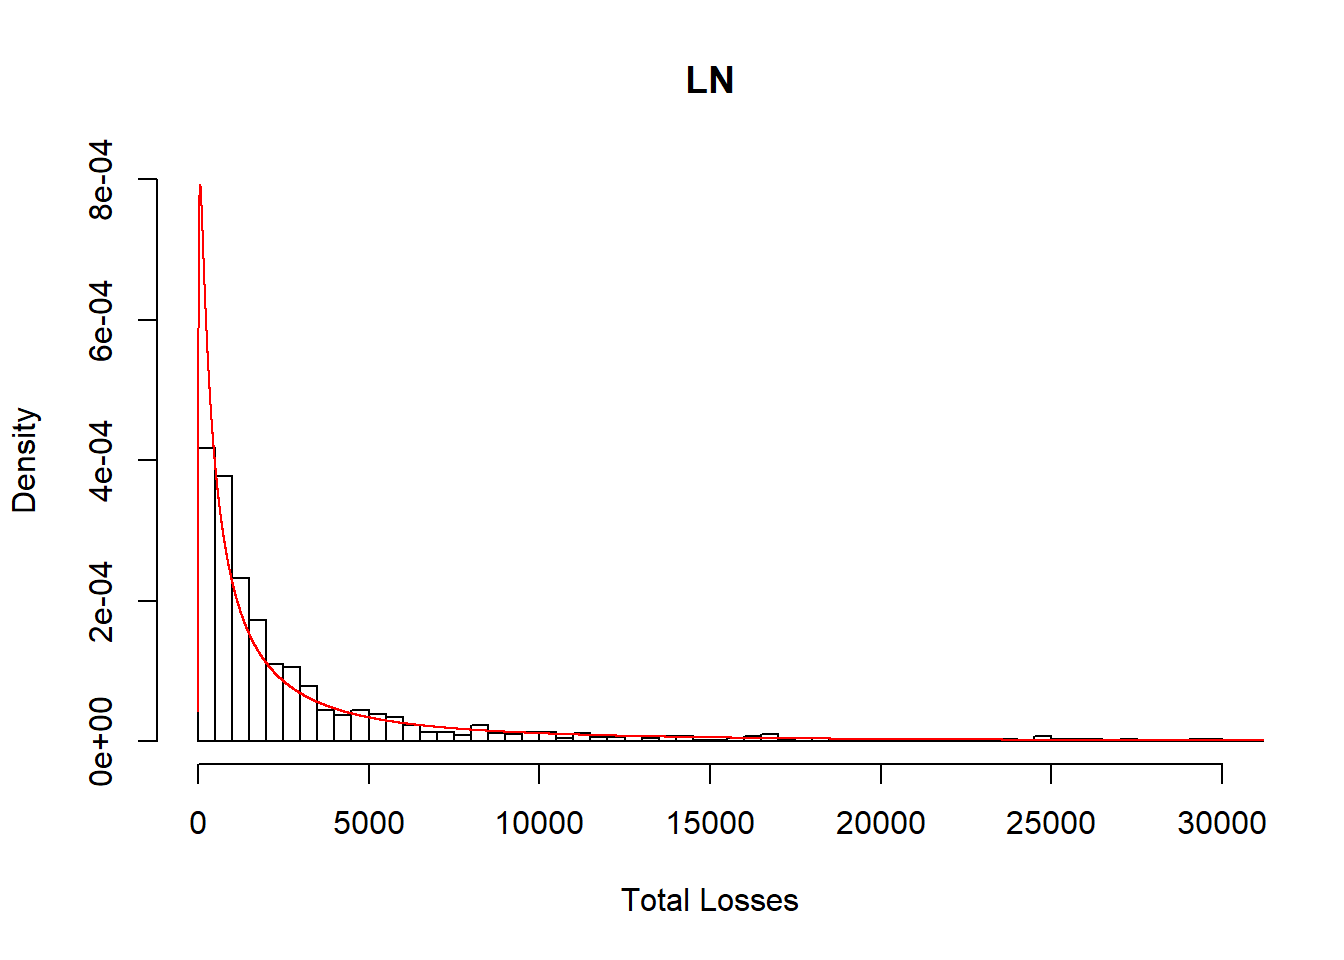
\includegraphics{R_for_Loss_Data_Analytics_files/figure-latex/unnamed-chunk-112-1} \end{center}

\subsubsection{Pareto}\label{pareto}

\begin{Shaded}
\begin{Highlighting}[]
\KeywordTok{hist}\NormalTok{(sev.dat}\OperatorTok{$}\NormalTok{Loss,}\DataTypeTok{xlab=}\StringTok{"Total Losses"}\NormalTok{,}\DataTypeTok{main=}\StringTok{"Pareto"}\NormalTok{,}\DataTypeTok{breaks=}\DecValTok{100}\NormalTok{,}\DataTypeTok{freq=}\NormalTok{F,}\DataTypeTok{xlim=}\KeywordTok{c}\NormalTok{(}\DecValTok{0}\NormalTok{,}\FloatTok{3e4}\NormalTok{),}\DataTypeTok{ylim=}\KeywordTok{c}\NormalTok{(}\DecValTok{0}\NormalTok{,}\FloatTok{8e-4}\NormalTok{))}
\NormalTok{x <-}\StringTok{ }\KeywordTok{seq}\NormalTok{(}\DecValTok{1}\NormalTok{,}\KeywordTok{max}\NormalTok{(sev.dat}\OperatorTok{$}\NormalTok{Loss),}\DecValTok{1}\NormalTok{)}
\NormalTok{theta <-}\StringTok{ }\NormalTok{zop.P}\OperatorTok{$}\NormalTok{par[}\DecValTok{1}\NormalTok{]}
\NormalTok{alpha <-}\StringTok{ }\NormalTok{zop.P}\OperatorTok{$}\NormalTok{par[}\DecValTok{2}\NormalTok{]}
\KeywordTok{lines}\NormalTok{(x,}\KeywordTok{dpareto}\NormalTok{(x,theta,alpha),}\DataTypeTok{col=}\StringTok{"blue"}\NormalTok{)}
\end{Highlighting}
\end{Shaded}

\begin{center}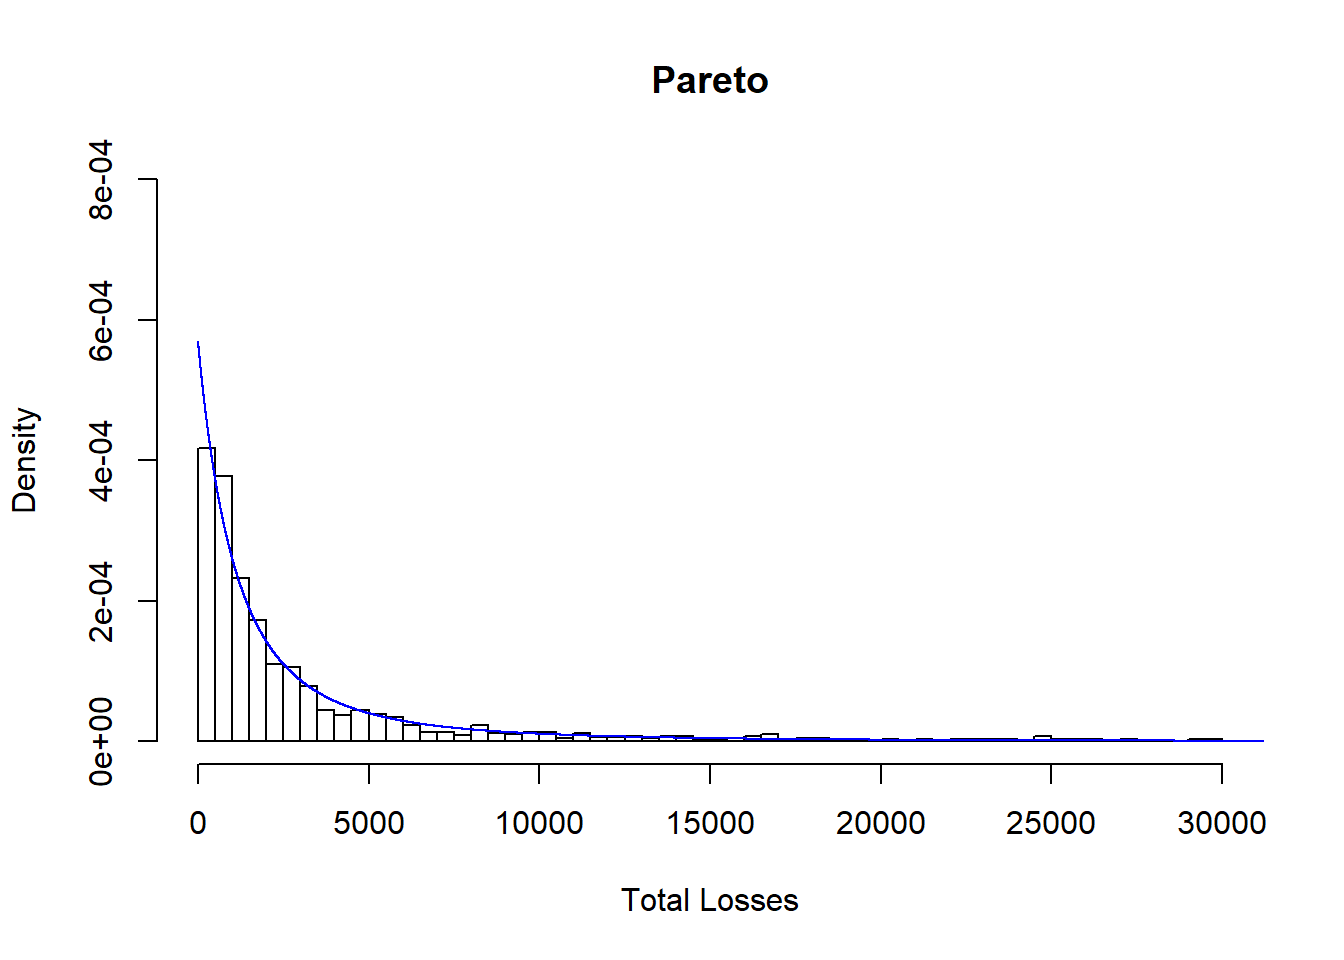
\includegraphics{R_for_Loss_Data_Analytics_files/figure-latex/unnamed-chunk-113-1} \end{center}

\subsection{qq Plots}\label{qq-plots}

\subsubsection{Define Quantile Function of
Pareto}\label{define-quantile-function-of-pareto}

\begin{Shaded}
\begin{Highlighting}[]
\NormalTok{qpareto <-}\StringTok{ }\ControlFlowTok{function}\NormalTok{(p,theta,alpha)\{theta}\OperatorTok{*}\NormalTok{((}\DecValTok{1}\OperatorTok{-}\NormalTok{p)}\OperatorTok{^}\NormalTok{(}\OperatorTok{-}\DecValTok{1}\OperatorTok{/}\NormalTok{alpha)}\OperatorTok{-}\DecValTok{1}\NormalTok{)\}}
\NormalTok{pct <-}\StringTok{ }\KeywordTok{seq}\NormalTok{(}\FloatTok{0.01}\NormalTok{,}\FloatTok{0.99}\NormalTok{,}\FloatTok{0.01}\NormalTok{)}
\KeywordTok{par}\NormalTok{(}\DataTypeTok{mfrow=}\KeywordTok{c}\NormalTok{(}\DecValTok{1}\NormalTok{,}\DecValTok{2}\NormalTok{))}
\KeywordTok{plot}\NormalTok{(}\KeywordTok{qlnorm}\NormalTok{(pct,mu,sigma),}\KeywordTok{quantile}\NormalTok{(sev.dat}\OperatorTok{$}\NormalTok{Loss,}\DataTypeTok{probs=}\NormalTok{pct),}
     \DataTypeTok{main=}\StringTok{"LN"}\NormalTok{, }\DataTypeTok{xlab=}\StringTok{"Theoretical Quantile"}\NormalTok{, }\DataTypeTok{ylab=}\StringTok{"Empirical Quantile"}\NormalTok{,}
     \DataTypeTok{xlim=}\KeywordTok{c}\NormalTok{(}\DecValTok{0}\NormalTok{,}\FloatTok{7.5e4}\NormalTok{),}\DataTypeTok{ylim=}\KeywordTok{c}\NormalTok{(}\DecValTok{0}\NormalTok{,}\FloatTok{7.5e4}\NormalTok{))}
\KeywordTok{abline}\NormalTok{(}\DecValTok{0}\NormalTok{,}\DecValTok{1}\NormalTok{)}
\KeywordTok{plot}\NormalTok{(}\KeywordTok{qpareto}\NormalTok{(pct,theta,alpha),}\KeywordTok{quantile}\NormalTok{(sev.dat}\OperatorTok{$}\NormalTok{Loss,}\DataTypeTok{probs=}\NormalTok{pct),}
     \DataTypeTok{main=}\StringTok{"Pareto"}\NormalTok{, }\DataTypeTok{xlab=}\StringTok{"Theoretical Quantile"}\NormalTok{, }\DataTypeTok{ylab=}\StringTok{"Empirical Quantile"}\NormalTok{,}
     \DataTypeTok{xlim=}\KeywordTok{c}\NormalTok{(}\DecValTok{0}\NormalTok{,}\FloatTok{7.5e4}\NormalTok{),}\DataTypeTok{ylim=}\KeywordTok{c}\NormalTok{(}\DecValTok{0}\NormalTok{,}\FloatTok{7.5e4}\NormalTok{))}
\KeywordTok{abline}\NormalTok{(}\DecValTok{0}\NormalTok{,}\DecValTok{1}\NormalTok{)}
\end{Highlighting}
\end{Shaded}

\begin{center}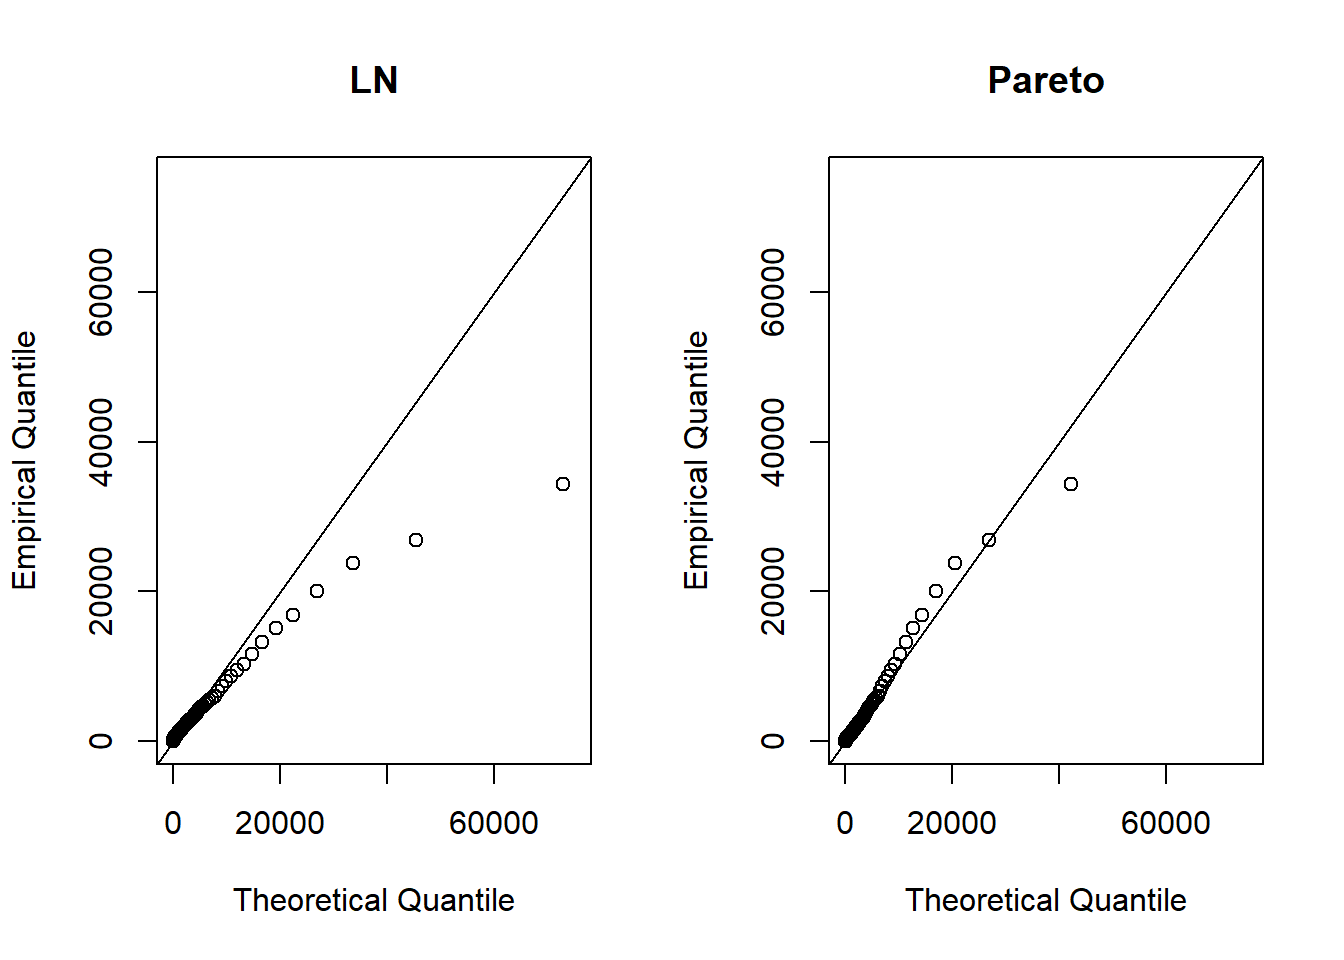
\includegraphics{R_for_Loss_Data_Analytics_files/figure-latex/unnamed-chunk-114-1} \end{center}

\chapter{Tweedie}\label{tweedie}

\emph{This file contains illustrative \textbf{R} code for the Tweedie
distribution. When reviewing this code, you should open an \textbf{R}
session, copy-and-paste the code, and see it perform. Then, you will be
able to change parameters, look up commands, and so forth, as you go. }

\section{Tweedie distribution}\label{tweedie-distribution}

\subsection{Load Tweedie Package}\label{load-tweedie-package}

First bring in the package Tweedie (you may need to first install this
package).

\begin{Shaded}
\begin{Highlighting}[]
\KeywordTok{library}\NormalTok{(tweedie)}
\end{Highlighting}
\end{Shaded}

\subsection{Set Paramteres for
Tweedie(p,mu,phi)}\label{set-paramteres-for-tweediepmuphi}

Setting parameters p, mu and phi defines the specific features of the
distribution.

Furthermore, setting a specific seed allows us to generate the same
randomn numbers so we can produce identical distributions

\begin{Shaded}
\begin{Highlighting}[]
\KeywordTok{set.seed}\NormalTok{(}\DecValTok{123}\NormalTok{)}
\NormalTok{p <-}\StringTok{ }\FloatTok{1.5}
\NormalTok{mu <-}\StringTok{ }\KeywordTok{exp}\NormalTok{(}\DecValTok{1}\NormalTok{) }
\NormalTok{phi <-}\StringTok{ }\KeywordTok{exp}\NormalTok{(}\DecValTok{1}\NormalTok{)}
\end{Highlighting}
\end{Shaded}

\subsection{Set Sample Size}\label{set-sample-size}

Sample size is set to 500 for this example. ``y'' holds all 500
obserations from tweedie distribution with the given parameters.

\begin{Shaded}
\begin{Highlighting}[]
\NormalTok{n <-}\StringTok{ }\DecValTok{500}
\NormalTok{y <-}\StringTok{ }\KeywordTok{rtweedie}\NormalTok{(n,p,mu,phi)}
\end{Highlighting}
\end{Shaded}

\subsection{Show Summary Statistics}\label{show-summary-statistics}

Here we calculate important statisitics like mean, median, standard
deviation and quantiles.

\begin{Shaded}
\begin{Highlighting}[]
\KeywordTok{summary}\NormalTok{(y)}
\end{Highlighting}
\end{Shaded}

\begin{verbatim}
   Min. 1st Qu.  Median    Mean 3rd Qu.    Max. 
  0.000   0.000   1.438   2.687   3.878  24.181 
\end{verbatim}

\begin{Shaded}
\begin{Highlighting}[]
\KeywordTok{sd}\NormalTok{(y)}
\end{Highlighting}
\end{Shaded}

\begin{verbatim}
[1] 3.346954
\end{verbatim}

\begin{Shaded}
\begin{Highlighting}[]
\KeywordTok{quantile}\NormalTok{(y,}\KeywordTok{seq}\NormalTok{(}\DecValTok{0}\NormalTok{,}\DecValTok{1}\NormalTok{,}\FloatTok{0.1}\NormalTok{))}
\end{Highlighting}
\end{Shaded}

\begin{verbatim}
        0%        10%        20%        30%        40%        50% 
 0.0000000  0.0000000  0.0000000  0.0000000  0.7275496  1.4378933 
       60%        70%        80%        90%       100% 
 2.3767214  3.4212150  5.2317625  7.7471281 24.1813833 
\end{verbatim}

\subsection{Show Histogram}\label{show-histogram}

Histograms are useful for visually interpreting data. Sometime summary
statistics aren't enough to see the full picture.

\begin{Shaded}
\begin{Highlighting}[]
\KeywordTok{hist}\NormalTok{(y, }\DataTypeTok{prob=}\NormalTok{T,}\DataTypeTok{breaks=}\DecValTok{50}\NormalTok{)}
\NormalTok{x <-}\StringTok{ }\KeywordTok{seq}\NormalTok{(}\DecValTok{0}\NormalTok{,}\KeywordTok{max}\NormalTok{(y),}\FloatTok{0.1}\NormalTok{)}
\KeywordTok{lines}\NormalTok{(x,}\KeywordTok{dtweedie}\NormalTok{(x,p,mu,phi),}\DataTypeTok{col=}\StringTok{"red"}\NormalTok{)}
\end{Highlighting}
\end{Shaded}

\begin{center}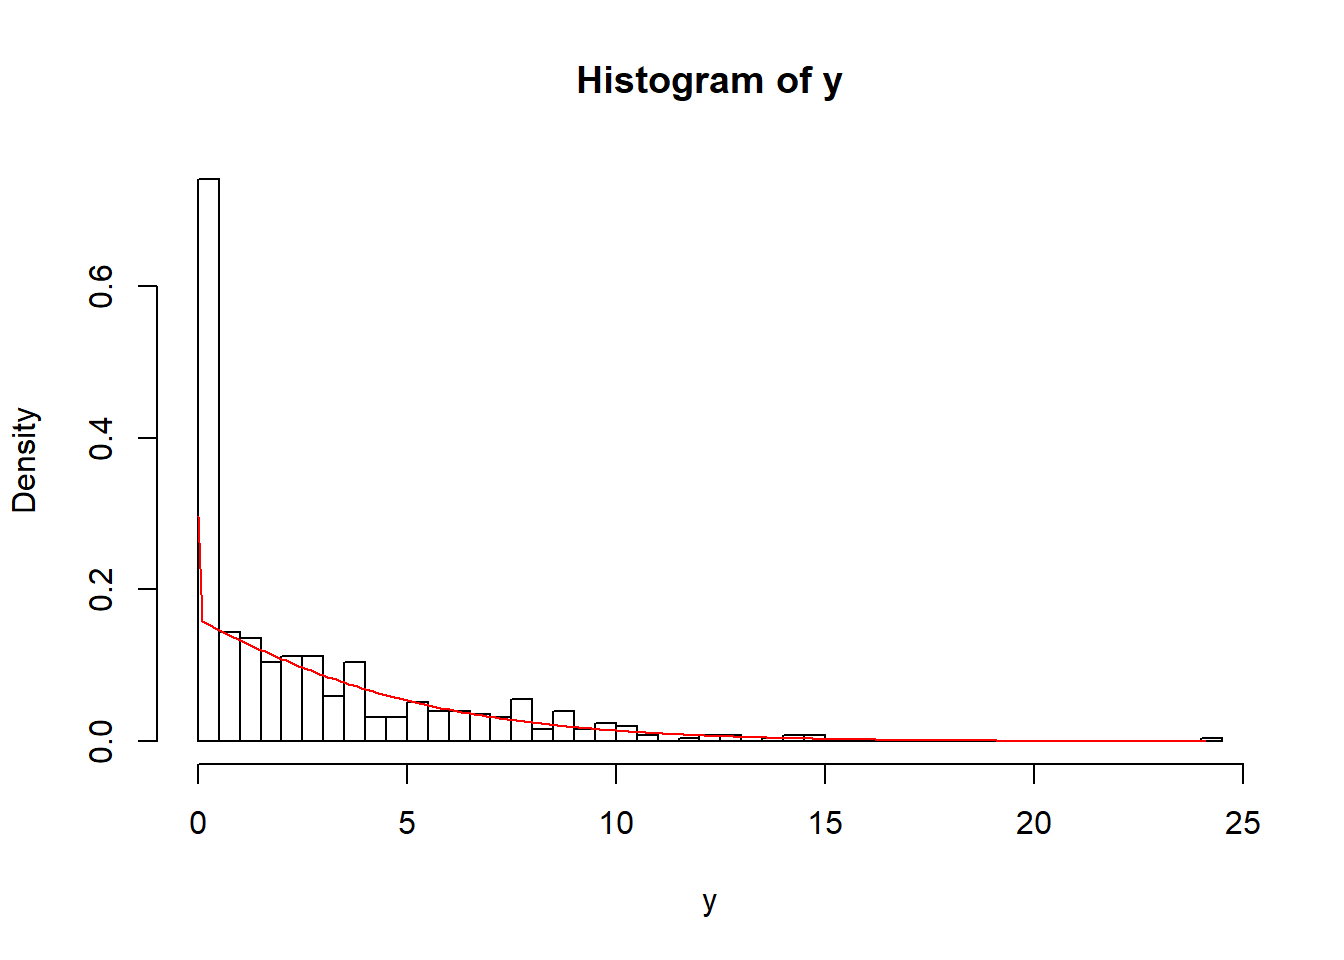
\includegraphics{R_for_Loss_Data_Analytics_files/figure-latex/unnamed-chunk-119-1} \end{center}

\subsection{QQ Plots for Different p
Values}\label{qq-plots-for-different-p-values}

A QQ plot is a plot of the quantiles of the first data set against the
quantiles of the second data set.

This is graphical technique for determining if two data sets come from
populations with a common distribution.

It appears here that a power of 1.5 matches the distribution best.

\begin{Shaded}
\begin{Highlighting}[]
\KeywordTok{par}\NormalTok{(}\DataTypeTok{mfrow=}\KeywordTok{c}\NormalTok{(}\DecValTok{2}\NormalTok{,}\DecValTok{2}\NormalTok{),}\DataTypeTok{mar=}\KeywordTok{c}\NormalTok{(}\DecValTok{4}\NormalTok{,}\DecValTok{4}\NormalTok{,}\DecValTok{4}\NormalTok{,}\DecValTok{4}\NormalTok{))}
\NormalTok{qqTweedie <-}\StringTok{ }\ControlFlowTok{function}\NormalTok{(xi,pct,mu,phi) \{}
  \KeywordTok{plot}\NormalTok{(}\KeywordTok{qtweedie}\NormalTok{(pct,xi,mu,phi),}\KeywordTok{quantile}\NormalTok{(y,}\DataTypeTok{probs=}\NormalTok{pct),}
       \DataTypeTok{main=}\KeywordTok{paste}\NormalTok{(}\StringTok{"Power = "}\NormalTok{,xi), }\DataTypeTok{xlab=}\StringTok{"Theoretical Quantile"}\NormalTok{, }\DataTypeTok{ylab=}\StringTok{"Empirical Quantile"}\NormalTok{)}
  \KeywordTok{abline}\NormalTok{(}\DecValTok{0}\NormalTok{,}\DecValTok{1}\NormalTok{)}
\NormalTok{\}}
\NormalTok{pct <-}\StringTok{ }\KeywordTok{seq}\NormalTok{(}\FloatTok{0.01}\NormalTok{,}\FloatTok{0.99}\NormalTok{,}\FloatTok{0.01}\NormalTok{)}
\KeywordTok{lapply}\NormalTok{(}\KeywordTok{c}\NormalTok{(}\DecValTok{1}\NormalTok{,}\FloatTok{1.5}\NormalTok{,}\DecValTok{2}\NormalTok{,}\FloatTok{2.5}\NormalTok{),qqTweedie,}\DataTypeTok{pct=}\NormalTok{pct,}\DataTypeTok{mu=}\NormalTok{mu,}\DataTypeTok{phi=}\NormalTok{phi)}
\end{Highlighting}
\end{Shaded}

\begin{center}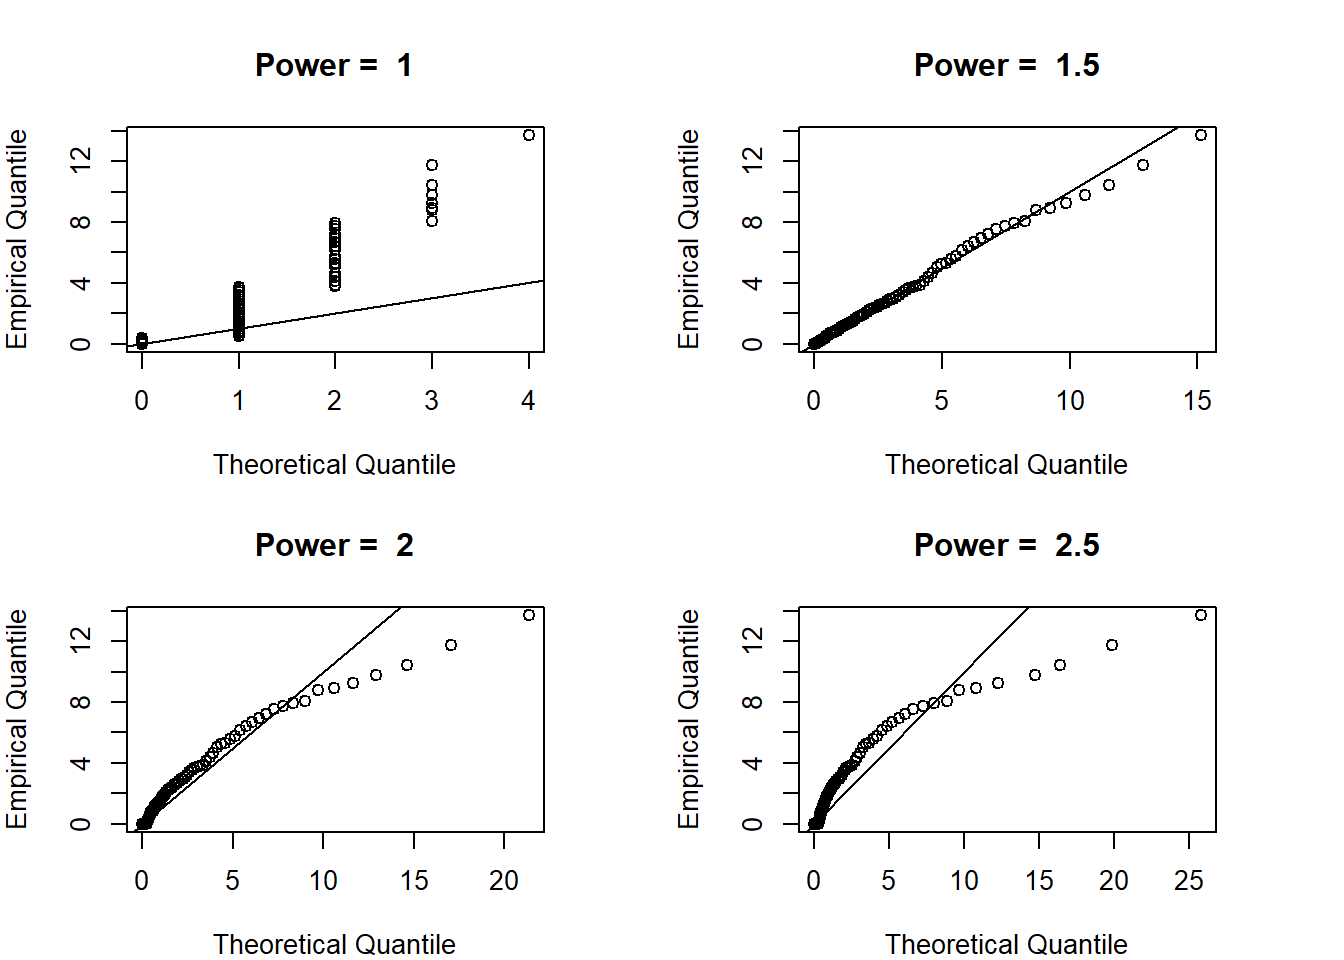
\includegraphics{R_for_Loss_Data_Analytics_files/figure-latex/unnamed-chunk-120-1} \end{center}

\begin{verbatim}
[[1]]
NULL

[[2]]
NULL

[[3]]
NULL

[[4]]
NULL
\end{verbatim}

\subsection{Fit Tweedie Distribution}\label{fit-tweedie-distribution}

Here we run a ``glm'' for the Tweedie distribution. you may need to
first install the ``statmod'' package

\begin{Shaded}
\begin{Highlighting}[]
\KeywordTok{library}\NormalTok{(statmod)}
\NormalTok{fit <-}\StringTok{ }\KeywordTok{glm}\NormalTok{(y}\OperatorTok{~}\DecValTok{1}\NormalTok{,}\DataTypeTok{family=}\KeywordTok{tweedie}\NormalTok{(}\DataTypeTok{var.power=}\FloatTok{1.5}\NormalTok{,}\DataTypeTok{link.power=}\DecValTok{0}\NormalTok{))}
\KeywordTok{summary}\NormalTok{(fit)}
\end{Highlighting}
\end{Shaded}

\begin{verbatim}

Call:
glm(formula = y ~ 1, family = tweedie(var.power = 1.5, link.power = 0))

Deviance Residuals: 
    Min       1Q   Median       3Q      Max  
-2.5607  -2.5607  -0.6876   0.5155   5.1207  

Coefficients:
            Estimate Std. Error t value Pr(>|t|)    
(Intercept)   0.9885     0.0557   17.75   <2e-16 ***
---
Signif. codes:  0 '***' 0.001 '**' 0.01 '*' 0.05 '.' 0.1 ' ' 1

(Dispersion parameter for Tweedie family taken to be 2.542861)

    Null deviance: 1618.8  on 499  degrees of freedom
Residual deviance: 1618.8  on 499  degrees of freedom
AIC: NA

Number of Fisher Scoring iterations: 4
\end{verbatim}

\subsection{Show Parameter Estimates}\label{show-parameter-estimates}

We now display the parameter estimates calculated in the glm.

\begin{Shaded}
\begin{Highlighting}[]
\KeywordTok{summary}\NormalTok{(fit)}\OperatorTok{$}\NormalTok{coefficient}
\end{Highlighting}
\end{Shaded}

\begin{verbatim}
             Estimate Std. Error  t value    Pr(>|t|)
(Intercept) 0.9885415  0.0556989 17.74795 5.42159e-55
\end{verbatim}

\begin{Shaded}
\begin{Highlighting}[]
\KeywordTok{summary}\NormalTok{(fit)}\OperatorTok{$}\NormalTok{dispersion}
\end{Highlighting}
\end{Shaded}

\begin{verbatim}
[1] 2.542861
\end{verbatim}

\subsection{Maximum Likelihood
Estimation}\label{maximum-likelihood-estimation}

Here we run a ``MLE'' to determine the most likely parameters of the
Tweedie distribution.

\begin{Shaded}
\begin{Highlighting}[]
\NormalTok{loglik<-}\ControlFlowTok{function}\NormalTok{(parms)\{ }
\NormalTok{  p=parms[}\DecValTok{1}\NormalTok{]}
\NormalTok{  mu=}\KeywordTok{exp}\NormalTok{(parms[}\DecValTok{2}\NormalTok{])}
\NormalTok{  phi=}\KeywordTok{exp}\NormalTok{(parms[}\DecValTok{3}\NormalTok{])}
\NormalTok{  llk <-}\StringTok{ }\OperatorTok{-}\KeywordTok{sum}\NormalTok{(}\KeywordTok{log}\NormalTok{(}\KeywordTok{dtweedie}\NormalTok{(y, p, mu, phi)))}
\NormalTok{  llk}
\NormalTok{\}}
\NormalTok{ini <-}\StringTok{ }\KeywordTok{c}\NormalTok{(}\FloatTok{1.5}\NormalTok{,}\DecValTok{1}\NormalTok{,}\DecValTok{1}\NormalTok{)}
\NormalTok{zop <-}\StringTok{ }\KeywordTok{nlminb}\NormalTok{(ini,loglik, }\DataTypeTok{lower =}\KeywordTok{c}\NormalTok{(}\DecValTok{1}\OperatorTok{+}\FloatTok{1e-6}\NormalTok{,}\OperatorTok{-}\OtherTok{Inf}\NormalTok{,}\OperatorTok{-}\OtherTok{Inf}\NormalTok{),}\DataTypeTok{upper =}\KeywordTok{c}\NormalTok{(}\DecValTok{2}\OperatorTok{-}\FloatTok{1e-6}\NormalTok{,}\OtherTok{Inf}\NormalTok{,}\OtherTok{Inf}\NormalTok{))}
\KeywordTok{print}\NormalTok{(zop)}
\end{Highlighting}
\end{Shaded}

\begin{verbatim}
$par
[1] 1.4823346 0.9885411 0.9871154

$objective
[1] 1122.992

$convergence
[1] 0

$iterations
[1] 14

$evaluations
function gradient 
      23       77 

$message
[1] "relative convergence (4)"
\end{verbatim}

\subsection{Obtain Standard Error}\label{obtain-standard-error-4}

Now we calculate the standard errors of our parameter estimates from the
MLE. You may need to first install the ``numDeriv'' package.

\begin{Shaded}
\begin{Highlighting}[]
\KeywordTok{library}\NormalTok{(numDeriv)}
\NormalTok{est <-}\StringTok{ }\NormalTok{zop}\OperatorTok{$}\NormalTok{par}
\KeywordTok{names}\NormalTok{(est) <-}\StringTok{ }\KeywordTok{c}\NormalTok{(}\StringTok{"p"}\NormalTok{,}\StringTok{"mu"}\NormalTok{,}\StringTok{"phi"}\NormalTok{)}
\NormalTok{hess<-}\KeywordTok{hessian}\NormalTok{(loglik,est)}
\NormalTok{se <-}\KeywordTok{sqrt}\NormalTok{(}\KeywordTok{diag}\NormalTok{(}\KeywordTok{solve}\NormalTok{(hess)))}
\KeywordTok{print}\NormalTok{(}\KeywordTok{cbind}\NormalTok{(est,se))}
\end{Highlighting}
\end{Shaded}

\begin{verbatim}
          est         se
p   1.4823346 0.02260226
mu  0.9885411 0.05672086
phi 0.9871154 0.05060983
\end{verbatim}

\chapter{Bootstrap Estimation}\label{bootstrap-estimation}

\emph{This file demonstrates both empirical and parametric boostrap
simulation. When reviewing this code, you should open an \textbf{R}
session, copy-and-paste the code, and see it perform. Then, you will be
able to change parameters, look up commands, and so forth, as you go.}

\section{Empirical Bootstrap}\label{empirical-bootstrap}

Example: 90\% confidence interval for the mean. Consider outcomes of
rolling a fair die.

\subsection{Random sample}\label{random-sample}

Here we input a sample of 10 observations, which we are going to build
our estimates off of.

\begin{Shaded}
\begin{Highlighting}[]
\NormalTok{y <-}\StringTok{ }\KeywordTok{c}\NormalTok{(}\DecValTok{1}\NormalTok{,}\DecValTok{3}\NormalTok{,}\DecValTok{2}\NormalTok{,}\DecValTok{5}\NormalTok{,}\DecValTok{4}\NormalTok{,}\DecValTok{5}\NormalTok{,}\DecValTok{5}\NormalTok{,}\DecValTok{6}\NormalTok{,}\DecValTok{6}\NormalTok{,}\DecValTok{6}\NormalTok{)}
\NormalTok{n <-}\StringTok{ }\KeywordTok{length}\NormalTok{(y)}
\NormalTok{n}
\end{Highlighting}
\end{Shaded}

\begin{verbatim}
[1] 10
\end{verbatim}

\subsection{Sample mean}\label{sample-mean}

Finding the mean of the random sample.

\begin{Shaded}
\begin{Highlighting}[]
\NormalTok{xbar <-}\StringTok{ }\KeywordTok{mean}\NormalTok{(y)}
\NormalTok{xbar}
\end{Highlighting}
\end{Shaded}

\begin{verbatim}
[1] 4.3
\end{verbatim}

\subsection{Random resamples from y}\label{random-resamples-from-y}

\subsubsection{Set bootstrap sample
size}\label{set-bootstrap-sample-size}

We're going to generate 30 different observations using the original
sample data, called the \emph{boostrap sample}

\begin{Shaded}
\begin{Highlighting}[]
\NormalTok{nboot <-}\StringTok{ }\DecValTok{30}
\NormalTok{tmpdata <-}\StringTok{ }\KeywordTok{sample}\NormalTok{(y,n}\OperatorTok{*}\NormalTok{nboot,}\DataTypeTok{replace=}\OtherTok{TRUE}\NormalTok{)}
\NormalTok{bootstrap.sample <-}\StringTok{ }\KeywordTok{matrix}\NormalTok{(tmpdata,}\DataTypeTok{nrow=}\NormalTok{n,}\DataTypeTok{ncol=}\NormalTok{nboot)}
\end{Highlighting}
\end{Shaded}

\subsubsection{Compute sample mean for each bootstrap
sample}\label{compute-sample-mean-for-each-bootstrap-sample}

Here we find the mean for all 30 of our boostrap samples.

\begin{Shaded}
\begin{Highlighting}[]
\NormalTok{bsmeans <-}\StringTok{ }\KeywordTok{colMeans}\NormalTok{(bootstrap.sample)}
\NormalTok{bsmeans}
\end{Highlighting}
\end{Shaded}

\begin{verbatim}
 [1] 3.8 4.8 4.5 4.4 4.4 4.3 4.5 4.5 5.2 4.6 3.5 4.1 4.6 4.3 4.5 4.9 4.6
[18] 4.0 4.8 4.0 4.5 4.0 4.8 4.3 4.2 4.6 3.3 3.4 4.4 3.6
\end{verbatim}

\subsection{90\% confidence interval}\label{confidence-interval}

Using the generated boostrap sample, we calculate a 90\% confidence
interval for our sample mean.

\begin{Shaded}
\begin{Highlighting}[]
\NormalTok{CI <-}\StringTok{ }\KeywordTok{c}\NormalTok{(}\KeywordTok{quantile}\NormalTok{(bsmeans,}\DataTypeTok{prob=}\FloatTok{0.05}\NormalTok{), }\KeywordTok{quantile}\NormalTok{(bsmeans,}\DataTypeTok{prob=}\FloatTok{0.95}\NormalTok{))}
\NormalTok{CI}
\end{Highlighting}
\end{Shaded}

\begin{verbatim}
   5%   95% 
3.445 4.855 
\end{verbatim}

\section{Parametric Bootstrap}\label{parametric-bootstrap}

Example: confidence interval for 1/theta. Consider y \textasciitilde{}
exponential(theta=10).

\subsection{random sample of size 250}\label{random-sample-of-size-250}

This time we generate a random sample of 250 observations from the
exponential sampling distribution.

\begin{Shaded}
\begin{Highlighting}[]
\NormalTok{y <-}\StringTok{ }\KeywordTok{rexp}\NormalTok{(}\DecValTok{250}\NormalTok{,}\DataTypeTok{rate=}\FloatTok{0.1}\NormalTok{)}
\NormalTok{n <-}\StringTok{ }\KeywordTok{length}\NormalTok{(y)}
\NormalTok{n}
\end{Highlighting}
\end{Shaded}

\begin{verbatim}
[1] 250
\end{verbatim}

\subsection{The MLE for lambda: 1/xbar}\label{the-mle-for-lambda-1xbar}

Remember from earlier that the MLE of theta for an exponential
distribution is its mean.

\begin{Shaded}
\begin{Highlighting}[]
\NormalTok{theta.mle <-}\StringTok{ }\KeywordTok{mean}\NormalTok{(y)}
\NormalTok{rate.hat <-}\StringTok{ }\DecValTok{1}\OperatorTok{/}\NormalTok{theta.mle}
\end{Highlighting}
\end{Shaded}

\subsection{Generate bootstrap
samples}\label{generate-bootstrap-samples}

Using the MLE we calculated we now generate 500 \emph{bootstrap samples}
of 250 observations each.

\begin{Shaded}
\begin{Highlighting}[]
\NormalTok{nboot <-}\StringTok{ }\DecValTok{500}
\NormalTok{tmpdata <-}\StringTok{ }\KeywordTok{rexp}\NormalTok{(n}\OperatorTok{*}\NormalTok{nboot,}\DataTypeTok{rate=}\NormalTok{rate.hat)}
\NormalTok{bootstrap.sample <-}\StringTok{ }\KeywordTok{matrix}\NormalTok{(tmpdata,}\DataTypeTok{nrow=}\NormalTok{n,}\DataTypeTok{ncol=}\NormalTok{nboot)}
\end{Highlighting}
\end{Shaded}

\subsection{compute botstrap
statistics}\label{compute-botstrap-statistics}

We now find the rate parameter for each of our \emph{boostrap samples}

\begin{Shaded}
\begin{Highlighting}[]
\NormalTok{rate.star <-}\StringTok{ }\DecValTok{1}\OperatorTok{/}\KeywordTok{colMeans}\NormalTok{(bootstrap.sample)}
\end{Highlighting}
\end{Shaded}

\subsection{calculate deviation from sample
statistics}\label{calculate-deviation-from-sample-statistics}

Subtracting the original sample rate parameter from each of our
simulated rate parameters, we can find the 5th and 95th percentiles of
the differences.

\begin{Shaded}
\begin{Highlighting}[]
\NormalTok{delta.star <-}\StringTok{ }\NormalTok{rate.star }\OperatorTok{-}\StringTok{ }\NormalTok{rate.hat}
\NormalTok{delta.lb <-}\StringTok{ }\KeywordTok{quantile}\NormalTok{(delta.star,}\DataTypeTok{prob=}\FloatTok{0.05}\NormalTok{)}
\NormalTok{delta.ub <-}\StringTok{ }\KeywordTok{quantile}\NormalTok{(delta.star,}\DataTypeTok{prob=}\FloatTok{0.95}\NormalTok{)}
\end{Highlighting}
\end{Shaded}

\subsection{90\% confidence intervel}\label{confidence-intervel}

We use the percentiles to create a 90\% CI for the rate parameter.

\begin{Shaded}
\begin{Highlighting}[]
\NormalTok{CI <-}\StringTok{ }\NormalTok{rate.hat }\OperatorTok{-}\StringTok{ }\KeywordTok{c}\NormalTok{(delta.ub,delta.lb)}
\KeywordTok{print}\NormalTok{(CI)}
\end{Highlighting}
\end{Shaded}

\begin{verbatim}
       95%         5% 
0.08817793 0.10884260 
\end{verbatim}

\bibliography{book.bib,packages.bib}


\end{document}
